% !TeX encoding = UTF-8
% !TeX program = xelatex
% !TeX spellcheck = en_US

\documentclass[degree=master]{thuthesis}
  % 学位 degree:
  %   doctor | master | bachelor | postdoc
  % 学位类型 degree-type:
  %   academic(默认)| professional


% 论文基本配置,加载宏包等全局配置
% !TeX root = ./thuthesis-example.tex

% 论文基本信息配置

\thusetup{
  %******************************
  % 注意:
  %   1. 配置里面不要出现空行
  %   2. 不需要的配置信息可以删除
  %   3. 建议先阅读文档中所有关于选项的说明
  %******************************
  %
  % 输出格式
  %   选择打印版(print)或用于提交的电子版(electronic),前者会插入空白页以便直接双面打印
  %
  output = print,
  %
  % 标题
  %   可使用“\\”命令手动控制换行
  %
  title  = {清华大学学位论文 \LaTeX{} 模板\\使用示例文档 v\version},
  title* = {An Introduction to \LaTeX{} Thesis Template of Tsinghua
            University v\version},
  %
  % 学位
  %   1. 学术型
  %      - 中文
  %        需注明所属的学科门类,例如:
  %        哲学、经济学、法学、教育学、文学、历史学、理学、工学、农学、医学、
  %        军事学、管理学、艺术学
  %      - 英文
  %        博士:Doctor of Philosophy
  %        硕士:
  %          哲学、文学、历史学、法学、教育学、艺术学门类,公共管理学科
  %          填写“Master of Arts“,其它填写“Master of Science”
  %   2. 专业型
  %      直接填写专业学位的名称,例如:
  %      教育博士、工程硕士等
  %      Doctor of Education, Master of Engineering
  %   3. 本科生不需要填写
  %
  degree-name  = {理学博士},
  degree-name* = {Doctor of Philosophy},
  %
  % 培养单位
  %   填写所属院系的全名
  %
  department = {物理系},
  %
  % 学科
  %   1. 学术型学位
  %      获得一级学科授权的学科填写一级学科名称,其他填写二级学科名称
  %   2. 工程硕士
  %      工程领域名称
  %   3. 其他专业型学位
  %      不填写此项
  %   4. 本科生填写专业名称,第二学位论文需标注“(第二学位)”
  %
  discipline  = {物理学},
  discipline* = {Physics},
  %
  % 姓名
  %
  author  = {丁伟},
  author* = {Ding Wei},
  %
  % 指导教师
  %   中文姓名和职称之间以英文逗号“,”分开,下同
  %
  supervisor  = {陈新, 副教授},
  supervisor* = {Professor Chen Xin},
  %
  % 副指导教师
  %
%  associate-supervisor  = {陈文光, 教授},
%  associate-supervisor* = {Professor Chen Wenguang},
  %
  % 联合指导教师
  %
  % joint-supervisor  = {某某某, 教授},
  % joint-supervisor* = {Professor Mou Moumou},
  %
  % 日期
  %   使用 ISO 格式;默认为当前时间
  %
  % date = {2019-07-07},
  %
  % 是否在中文封面后的空白页生成书脊(默认 false)
  %
  include-spine = false,
  %
  % 密级和年限
  %   秘密, 机密, 绝密
  %
  % secret-level = {秘密},
  % secret-year  = {10},
  %
  % 博士后专有部分
  %
  % clc                = {分类号},
  % udc                = {UDC},
  % id                 = {编号},
  % discipline-level-1 = {计算机科学与技术},  % 流动站(一级学科)名称
  % discipline-level-2 = {系统结构},          % 专业(二级学科)名称
  % start-date         = {2011-07-01},        % 研究工作起始时间
}

% 载入所需的宏包

% 可以使用 nomencl 生成符号和缩略语说明
% \usepackage{nomencl}
% \makenomenclature

% 表格加脚注
\usepackage{threeparttable}

% 表格中支持跨行
\usepackage{multirow}

% 固定宽度的表格。
% \usepackage{tabularx}

% 跨页表格
\usepackage{longtable}

% 量和单位
\usepackage{siunitx}

% 定理类环境宏包
\usepackage{amsthm}
% 也可以使用 ntheorem
% \usepackage[amsmath,thmmarks,hyperref]{ntheorem}

% 参考文献使用 BibTeX + natbib 宏包
% 顺序编码制
\usepackage[sort]{natbib}
\bibliographystyle{thuthesis-numeric}

% 著者-出版年制
% \usepackage{natbib}
% \bibliographystyle{thuthesis-author-year}

% 本科生参考文献的著录格式
% \usepackage[sort]{natbib}
% \bibliographystyle{thuthesis-bachelor}

% 参考文献使用 BibLaTeX 宏包
% \usepackage[backend=biber,style=thuthesis-numeric]{biblatex}
% \usepackage[backend=biber,style=thuthesis-author-year]{biblatex}
% \usepackage[backend=biber,style=apa]{biblatex}
% \usepackage[backend=biber,style=mla-new]{biblatex}
% 声明 BibLaTeX 的数据库
% \addbibresource{ref/refs.bib}

% 定义所有的图片文件在 figures 子目录下
\graphicspath{{figures/}}

% 数学命令
\newcommand\dif{\mathop{}\!\mathrm{d}}  % 微分符号

% hyperref 宏包在最后调用
\usepackage{hyperref}


%WEI 

\usepackage{makecell}
\usepackage{adjustbox}
\usepackage{amsmath}
\DeclareMathOperator{\sech}{sech}



\begin{document}

% 封面
\maketitle

% 学位论文指导小组、公开评阅人和答辩委员会名单
% !TeX root = ../thuthesis-example.tex

\begin{committee}[name={学位论文指导小组、公开评阅人和答辩委员会名单}]

  \newcolumntype{C}[1]{@{}>{\centering\arraybackslash}p{#1}}

  \section*{指导小组名单}

  \begin{center}
    \begin{tabular}{C{3cm}C{3cm}C{9cm}@{}}
      李XX & 教授     & 清华大学 \\
      王XX & 副教授   & 清华大学 \\
      张XX & 助理教授 & 清华大学 \\
    \end{tabular}
  \end{center}


  \section*{公开评阅人名单}

  \begin{center}
    \begin{tabular}{C{3cm}C{3cm}C{9cm}@{}}
      刘XX & 教授   & 清华大学                    \\
      陈XX & 副教授 & XXXX大学                    \\
      杨XX & 研究员 & 中国XXXX科学院XXXXXXX研究所 \\
    \end{tabular}
  \end{center}


  \section*{答辩委员会名单}

  \begin{center}
    \begin{tabular}{C{2.75cm}C{2.98cm}C{4.63cm}C{4.63cm}@{}}
      主席 & 赵XX                  & 教授                    & 清华大学       \\
      委员 & 刘XX                  & 教授                    & 清华大学       \\
          & \multirow{2}{*}{杨XX} & \multirow{2}{*}{研究员} & 中国XXXX科学院 \\
          &                       &                         & XXXXXXX研究所  \\
          & 黄XX                  & 教授                    & XXXX大学       \\
          & 周XX                  & 副教授                  & XXXX大学       \\
      秘书 & 吴XX                  & 助理研究员              & 清华大学       \\
    \end{tabular}
  \end{center}

\end{committee}



% 也可以导入 Word 版转的 PDF 文件
% \begin{committee}[file=figures/committee.pdf]
% \end{committee}


% 使用授权的说明
\copyrightpage
% 将签字扫描后授权文件 scan-copyright.pdf 替换原始页面
% \copyrightpage[file=scan-copyright.pdf]

\frontmatter
% !TeX root = ../main.tex

% 中英文摘要和关键字

\begin{abstract}
  
位于欧洲的大型强子对撞机(LHC)的两个主要的目标是标准模型的精确测量和寻找超出标准模型的新物理。
随着2012年标准模型中最后一个粒子希格斯玻色子的发现,
与希格斯玻色子相关的性质测量变得非常重要,
其中$H\to b\bar{b}$是希格斯玻色子主要的衰变模式。
在LHC上的ATLAS实验中,
高横动量$H\to b\bar{b}$衰变过程是通过一个距离参数R=1的LR-jet重建出来的,
随后在这个LR-jet中重建出带有味标定信息的subjet。
这篇论文展示了一种用于标定高横动量$H\to b\bar{b}$事例的新算法,
新算法是基于一个前馈型神经网络,
以LR-jet的动力学变量以及其中subjet的味标定区分因子为输入进行训练得到的,
它不仅对LR-jet的质量没有明显的影响,而且相对于其他基线算法,
它能更有效的排除来自于QCD过程和高横动量t夸克衰变的本底。

同时,在寻找超出标准模型的新物理方面,
这篇论文还展示了,
利用ATLAS从2015年到2018年在质心系能量为$\sqrt{s}$=13TeV下收集到的总积分亮度为139$fb^{-1}$的质子-质子对撞数据,
在事例中两个横动量最高的jet的不变质量谱中寻找衰变末态为两个jet的新共振态,其中包含末态jet被标记为b-jet的信号道。
在平滑下降的标准模型本底上,没有发现显著的新物理信号,
并对一系列基准信号在95\%置信度下设置了更强的排除限,包括模型无关的高斯信号。
在衰变末态包含b-jet的信号道,
得益于在高横动量下b-jet标定算法的显著改进,
相对于上一轮分析,除了因积分亮度提高带来的增益之外,
灵敏度在此基础上有了更大的提升。







  % 关键词用“英文逗号”分隔
  \thusetup{
    keywords = {大型强子对撞机,ATLAS实验,标准模型,希格斯玻色子,b夸克,暗物质,神经网络},
  }
\end{abstract}

\begin{abstract*}

Two of the most important targets of the Large Hadron Collider(LHC) is the precision measurement of the Standard Model and 
the search for Beyond Standard Model particles and interactions.
In 2012, the ATLAS and CMS experiments completed the search for Standard Model particles with the discovery of the Higgs boson,
then the precision measurement of the properties of the Higgs boson becomes really important.
Boosted Higgs bosons decaying via the dominant $H\to b\bar{b}$ mode are an essential ingredient to a number of LHC physics signatures,
ATLAS identifies these hadronic Higgs bosons by reconstructing a large-R jet with R=1, associating variable-radius subjets to the large-R jet,
and then assigning a flavor discriminant to each of the subjets using standard flavor tagging.
This thesis presents an algorithm to select boosted Higgs bosons that combines flavor discriminants from up to three subjets using a feed-forward neural network.
In addition to the decorrelation from the large-R jet mass,
a comparison of several algorithms that combine individual subjet discriminants show that the neural network-based algorithm is the most powerful, 
assessed on its ability to reject both boosted top quark jets and jets arising from QCD processes. 

In the meantime, for the Beyond Standard Model search,
this thesis also presents a search for new resonances decaying into a pair of jets 
using the dataset of proton--proton collisions recorded at $\sqrt{s}$=13TeV with the ATLAS detector at the LHC between 2015 and 2018, corresponding to an integrated luminosity of 139fb$^{-1}$.
The distribution of the invariant mass of the two leading jets is examined for local excesses above a data-derived estimate of the Standard Model background.
In addition to an inclusive search, events with jets identified as containing $b$-hadrons are examined specifically,
no significant excess of events above the smoothly falling background spectra is observed.
The results are used to set cross-section upper limits at 95\% confidence level on a range of new physics scenarios, model-independent limits on Gaussian-shaped signals are also reported.
The analysis looking at jets containing $b$-hadrons benefits from improvements in the jet flavour identification at high transverse momentum, 
which increases its sensitivity relative to the previous analysis beyond that expected from the higher integrated luminosity.




  \thusetup{
    keywords* = {LHC, ATLAS, the Standard Model ,Higgs boson , b-tagging ,Dark Matter},
  }
\end{abstract*}


% 目录
\tableofcontents

% 插图和附表清单
\listoffiguresandtables  % 插图和附表清单
% \listoffigures           % 插图清单
% \listoftables            % 附表清单

% 符号对照表
% !TeX root = ../main.tex

\begin{denotation}[3cm]
\item[CERN] 欧洲核子研究中心(The European Organization for Nuclear Research)
\item[LHC] 大型强子对撞机(The Large Hadron Collider)
\item[ATLAS] 环形LHC设备(A Toroidal LHC ApparatuS)
\item[CMS] 紧凑型$\mu$子螺线管(The Compact Muon Solenoid)
\item[SM] 标准模型(The Standard Model)
\item[QFT] 量子场论(Quantum Field Theory)
\item[q] 夸克(Quark)
\item[g] 胶子(Gluon)
\item[CPT] 电荷、宇称和时间反演对称(Charge、parity and time reversal symmetry)
\item [QED] 量子电动力学(Quantum electrodynamics)
\item[QCD] 量子色动力学(Quantum chromodynamics)
\item[EW] 电弱理论(Electroweak theory)
\item[CKM] Cabibbo–Kobayashi–Maskawa
\item[SSB] 对称性自发破缺(Spontaneous symmetry breaking)
\item[BR] 分支比(Branching ratio)
\item[BSM] 超出标准模型的新物理(Physics beyond the Standard Model )
\item[DM] 暗物质(Dark Matter)
\item[SSM] 连续标准模型(The Sequential Standard Model)
\item[KK] Kaluza-Klein
\item[G] 引力子(Graviton)
\item[ggF] 胶子融合(Gluon–gluon fusion)
\item[VBF] 矢量玻色子融合(Vector-boson fusion)
\item[jet] 喷注
\item[b-jet] 含b强子的喷注
\item[LR-jet] 距离参数R=1的大喷注(Large-R jet)
\item[subjet] 包含在距离参数R=1的大喷注内部的喷注
\item[MC] Monte Carlo
\item[PDF] 部分子分布函数(Parton Distribution Functions)
\item[PD] 像素探测器(The Pixel Detector)
\item[SCT] 半导体径迹探测器(The SemiConductor Tracker)
\item[DNN] 深度学习神经网络(Deep Neural Network)
\item[BDT] 提升决策树(Boosted Decision Tree)
\item[JSS] LR-jet的结构变量(Jet substructure)
\item[FR-jet] 由距离参数R=0.2的anti-$k_t$算法基于径迹重建出来的喷注(Fixed radius track jet)
\item[VR-jet] 由距离参数R可变的anti-$k_t$算法基于径迹重建出来喷注(Variable radius track jet)
\item[TH-jet] 由anti-$k_t$算法基于产生子层面真实粒子的径迹重建出来的喷注(Truth jet)
\item[LO] 领头阶(Leading order)
\item[JES] 喷注能量刻度(Jet energy scale)
\item[JER] 喷注分辨率(Jet energy resolution)
\item[dijet] 双喷注
\end{denotation}



% % 也可以使用 nomencl 宏包:

% \printnomenclature[3cm]

% \nomenclature{HPC}{高性能计算 (High Performance Computing)}
% \nomenclature{cluster}{集群}
% \nomenclature{Itanium}{安腾}
% \nomenclature{SMP}{对称多处理}
% \nomenclature{API}{应用程序编程接口}
% \nomenclature{PI}{聚酰亚胺}
% \nomenclature{MPI}{聚酰亚胺模型化合物,N-苯基邻苯酰亚胺}
% \nomenclature{PBI}{聚苯并咪唑}
% \nomenclature{MPBI}{聚苯并咪唑模型化合物,N-苯基苯并咪唑}
% \nomenclature{PY}{聚吡咙}
% \nomenclature{PMDA-BDA}{均苯四酸二酐与联苯四胺合成的聚吡咙薄膜}
% \nomenclature{$\increment G$}{活化自由能 (Activation Free Energy)}
% \nomenclature{$\chi$}{传输系数 (Transmission Coefficient)}
% \nomenclature{$E$}{能量}
% \nomenclature{$m$}{质量}
% \nomenclature{$c$}{光速}
% \nomenclature{$P$}{概率}
% \nomenclature{$T$}{时间}
% \nomenclature{$v$}{速度}



% 正文部分
\mainmatter
% !TeX root = ../main.tex

\chapter{绪论}
\label{cha:intro}

一直以来,很多物理学家在尝试找到一个可以统一自然界和整个宇宙的所有物质和现象的“终极理论”,
并希望它能解释所有已知的物质和相互作用及其基本结构,小到质子中子,大到银河系或者整个宇宙;
它能追溯宇宙的起源,关于宇宙的存在和宇宙是怎么产生的;
它也能对某些现象进行预测等等。
早在十九世纪初期,随着爱因斯坦狭义相对论的提出~\cite{SRE}和量子力学~\cite{QMP}的发现,经典物理的基础被动摇。
狭义相对论迫使科学家改变了他们对时间和空间的认知,时间和空间是不可分割的交织在一起的,
是单一现实的不同两个方面,即时空;量子力学让科学家们看到微观世界的运动规律和宏观世界如此不一样,
粒子的行为表现的像场,而场的行为也类似于粒子。
到十九世纪中期,狄拉克将量子力学和狭义相对论完美的融合在了一起~\cite{QMP},
随后科学家们将它们与经典场论结合起来形成了一种功能强大的物理框架,量子场论~\cite{QFT1}。
同时,以量子场论作为基本框架,标准模型~\cite{SM2}也随之萌芽,一个与“终极理论”最为接近的物理模型,
十九世纪后半叶便是标准模型随着各式的高能物理实验一起发展、逐渐完善的过程。
而对称性在标准模型的发展过程中一直扮演着重要角色,
这起源于早期外尔发现了电磁相互作用中的规范对称性~\cite{WEYL},在科学家们发现夸克之后,
一种隐藏在夸克内部的“颜色”对称性逐渐浮出水面~\cite{SM0},
对应于一种束缚质子和中子中夸克的作用力,强相互作用。
随后的一个重大突破便是科学家们意识到对称性或许可以自发的破坏~\cite{SM4,SM5,SM6},
到后来二十世纪末期W、Z玻色子和二十一世纪初期“上帝粒子”希格斯玻色子的发现~\cite{ZBOSON,WBOSON1,WBOSON2,ATLASHIGGS,CMSHIGGS},
验证了对称性自发破缺这个设想的正确性,这也代表着标准模型的巨大成功,
到目前为止,所有已知的粒子都具有该模型所精确预测的性质。
与此同时,科学家们对标准模型也提出了很多新问题,
为什么不包含引力?暗物质从何而来?为什么夸克分为六个味而且质量差异如此之大?等等,
因此对超出标准模型的新物理的研究仍然具有重要的意义。

目前,欧洲核子研究中心(The European Organization for Nuclear Research, CERN)的大型强子对撞机(The Large Hadron Collider, LHC)~\cite{Evans:2008zzb}作为全世界最大的粒子物理实验室,开展着一系列该领域的前沿研究,
其中两个重要的方面就是与希格斯玻色子相关的性质测量和超出标准模型的新物理的寻找,
这篇论文的研究工作便是在这个背景下完成的,
论文工作主要集中在两个方面:
基于LHC的ATLAS(A Toroidal LHC ApparatuS)探测器~\cite{PERF-2007-01}中高横动量希格斯玻色子衰变到双b夸克的标定和在双喷注末态的不变质量谱中寻找超出标准模型的新物理。
具体的章节安排为:
第~\ref{cha:intro}~章简要的介绍研究背景;
第~\ref{cha:Theory}~章介绍研究工作的理论背景,包括标准模型、希格斯玻色子的性质、
研究工作的动机和与研究工作相关的超出标准模型的新物理模型;
第~\ref{cha:EXP}~章着重于实验技术,首先会简要介绍一下LHC,然后详细介绍LHC上的ATLAS探测器及其各个组成部分,
随后简要介绍模拟实现技术和ATLAS探测器中物理对象的重建技术;
第~\ref{cha:ML}~章会简要介绍高能物理实验领域常用的两种机器学习算法:神经网络和提升决策树,其中第~\ref{cha:Xbb}~章的研究工作便是以神经网络为基础的;
第~\ref{cha:Xbb}~章详细介绍了高横动量希格斯玻色子衰变到双b夸克的标定算法的开发动机、研究现状、设计思路、性能及其与ATLAS合作组已有算法的对比等,%及其与ATLAS合作组已有算法的对比等,
这部分研究工作已经以公告文章(ATLAS public note)的形式发表出来~\cite{ATL-PHYS-PUB-2020-019};
第~\ref{cha:Dijet}~章详细介绍了物理分析在双喷注末态的不变质量谱中寻找超出标准模型的新物理的动机、研究现状、技术手段和实验结果等,
这部分研究工作的结果最近发表在高能物理杂志(Journal of High Energy Physics, JHEP)上面~\cite{DijetPaper};%并且我在其中作为分析的主力成员之一
最后第~\ref{cha:Summary}~章是研究工作的总结和展望部分。













% !TeX root = ../main.tex

\chapter{理论}
\label{cha:Theory}

粒子物理是物理学的一个分支,是研究组成物质世界的
%不可分割的最小可检测的
最基本的粒子和它们之间相互作用的一门学科,
目前解释已知的基本粒子和它们之间相互作用的动力学的
%主要的也是
最成功的理论是标准模型(The Standard Model, SM)
~\cite{SM1,SM2,SM3,SM4,SM5,SM6,SM7,SMTALK,SM8,SMBOOK}。
从1897年J.J.Thomson首次在实验中发现电子~\cite{THOMSON},到2012年标准模型中最后一个粒子希格斯玻色子的发现~\cite{ATLASHIGGS,CMSHIGGS},
标准模型经过一百多年的发展逐渐完善,其不仅理论上自洽,而且在实验预测上也非常的成功。
尽管如此,物理学家在
%理论和实验研究中
试图将其扩展成为一个包含所有常数和物理现象的“终极理论”的时候,
发现仍有一些不足之处亟待解决,比如标准模型没有解释暗物质~\cite{DARKMATTER1,DARKMATTER2}从何而来、没有包含引力子~\cite{GRAVITON}、
也没有解释宇宙中正反物质不对称~\cite{ANTIMATTER}和中微子质量起源~\cite{NEUTRINO1,NEUTRINO2}等问题。

本章第~\ref{sec:SM}~小节将简要介绍标准模型,包括各种相互作用、对称性自发破缺和希格斯玻色子,
接着在第~\ref{sec:Higgs}~小节会介绍希格斯玻色子的性质和高横动量希格斯玻色子衰变到双b夸克的标定动机,
最后第~\ref{sec:BSM}~小节简要介绍在双喷注末态的不变质量谱中寻找超出标准模型的新物理的动机和所用到的基准新物理模型。

\section{标准模型}
\label{sec:SM}


由于覆盖范围广、预测能力强以及对已知的基本粒子之间相互作用的精确描述,
粒子物理中的标准模型被认为是现有最全面而且最强大的物理理论之一。
它的目标是对亚原子粒子进行分类,并准确描述它们之间的相互作用和自相互作用,
类似于元素周期表,标准模型可以根据其属性对所有已知的基本粒子进行排布。
量子场论(Quantum Field Theory, QFT)~\cite{QFT1}是严格描述和构建标准模型的数学基础,
它协调了量子力学~\cite{QMP}和狭义相对论~\cite{SRE},
在这个基础之上,粒子被视为相应场的量子化激发,
而场是将标量、矢量或张量与时空中每个点关联起来的函数,
相互作用可以通过各种场的理论来描述。
标准模型的构建遵循对称性原则,而拉格朗日量是描述物理系统动力学的基本手段,又称拉氏量,
因此物理体系的基本对称性是通过体系拉氏量的对称性来体现的。
与理论相联系的实验观测量比如散射截面和衰变宽度等可以利用
微扰论的方法得到~\cite{QFT1}。

\subsection{最小作用量原理}
\label{sec:LAP}
类似于经典力学,物理系统的动力学特征可以由最小作用量原理~\cite{ACTION1,ACTION2}得到,
首先,定义一个体系的作用量S:
\begin{equation} 
\label{eq:ACTION1}
S=\int d^4x \quad \mathcal{L}\left[ \phi_i(x),\partial_{\mu}\phi_i(x) \right]
\end{equation}
其中四维时空的积分$\int d^4x$保持洛伦兹不变性,
体系的拉氏量密度$\mathcal{L}$是场$\phi_i(x)$和它们的偏导$\partial_{\mu}\phi_i(x)$的函数,
它也具有洛伦兹不变性。
最小作用量原理要求作用量的变化$\delta S$在场的微小变化$\delta \phi_i$之下为零,
假设$\delta \phi_i$是可微的并且在时空的某个有界区域之外为零,
由$\delta S=0$可以得到场的欧拉-拉格朗日运动方程:
\begin{equation} 
\label{eq:ACTION2}
\frac{\partial\mathcal{L}}{\partial\phi_i}-\partial^{\mu}\left( \frac{\mathcal{L}}{\partial(\partial^{\mu}\phi_i)} \right) =0
\end{equation}

\subsection{对称性和守恒律}
\label{sec:SCL}
假设在一组连续的变换下:
\begin{equation} 
\label{eq:ACTION3}
\phi_i(x) \rightarrow \phi'_i(x)=\phi_i(x)+\epsilon\delta_{\epsilon}\phi_i(x)+O(\epsilon^2)
\end{equation}
体系的拉氏量保持不变:
\begin{equation} 
\label{eq:ACTION4}
\mathcal{L}\left[ \phi_i(x),\partial_{\mu}\phi_i(x) \right]=\mathcal{L}\left[ \phi'_i(x),\partial_{\mu}\phi'_i(x) \right]
\end{equation}
那么可以得到:
\begin{equation} 
\label{eq:ACTION5}
\delta_{\epsilon}\mathcal{L} \quad = \quad 0 \quad = \quad \sum_i \Bigg\{ \left[ \frac{\partial\mathcal{L}}{\partial\phi_i}-\partial^{\mu}\left( \frac{\partial\mathcal{L}}{\partial(\partial^{\mu}\phi_i)} \right) \right] \delta_{\epsilon}\phi_i + \partial^{\mu}  \left[  \frac{\partial\mathcal{L}}{\partial(\partial^{\mu}\phi_i)}\delta_{\epsilon}\phi_i  \right]   \Bigg\}
\end{equation}
上式右边第一项便是欧拉-拉格朗日运动方程~\ref{eq:ACTION2}~,其值为零,
化简之后,体系有一个守恒流:
\begin{equation} 
\label{eq:ACTION6}
J_{\mu}\equiv\sum_i \frac{\mathcal{L}}{\partial(\partial^{\mu}\phi_i)}\delta_{\epsilon}\phi_i , \quad \partial^{\mu}J_{\mu}=0
\end{equation}
其中第一项定义为守恒荷:
\begin{equation} 
\label{eq:ACTION7}
Q \equiv \int d^3x J^0
\end{equation}
式~\ref{eq:ACTION6}~中的条件$\partial^{\mu}J_{\mu}=0$保证了$\frac{dQ}{dt}=0$,因此Q是个守恒量。
这种关系被称为Noether定理~\cite{NOETHER},
%可以将其扩展到
在涉及时空坐标的一般变换中,
对于每一个使作用量保持不变的连续对称变换,
都会出现一个相应的守恒流,因此也会有一个守恒荷。

标准模型包含了三种基本的相互作用:强相互作用、弱相互作用和电磁相互作用。
这三种基本相互作用的构建是基于三种不同的对称性,
与基本的相互作用关联的这些对称性被称为局部规范对称性,
对称性的数学基础是群论~\cite{GROUP},
从而,标准模型是通过三个代表对称性的群$SU(3)	\otimes SU(2)	\otimes U(1)$构建起来的:
%对称群$SU(3)$反应的是强相互作用的对称性,
强相互作用的对称性群是$SU(3)$,由量子色动力学描述,
与这个对称性相对应的守恒荷为色荷;
%对称群$SU(2)	\otimes U(1)$反应的是电磁和弱相互作用的对称性
电磁和弱相互作用的对称性群$SU(2)	\otimes U(1)$,用电弱理论描述;
电磁相互作用的对称性群为$U(1)$,由量子电动力学描述,
与这个对称性相对应的守恒荷为电荷。

%$U(1)$可以单独描述电磁相互作用的对称性,相应的理论为量子电动力学,守恒荷为电荷。
另外,由狭义相对论的要求,标准模型需满足最基本的洛伦兹对称性,这种对称性是全局对称性,
相应的对称性群为洛伦兹群,由于洛伦兹群特殊的拓扑性质,
标准模型对基本粒子分类时需引入一个被称为自旋的内禀属性~\cite{QFT1},它只能取整数或者半整数,
自旋为半整数的粒子被称为费米子,自旋为整数的粒子被称为玻色子。
标准模型中的质量也是粒子的一个内禀属性,
它是由粒子所对应的场与希格斯玻色子所对应的场的耦合引起的,
其中希格斯玻色子是标准模型中唯一一个自旋为0的基本粒子,后文将会介绍。
这里引入这些基本属性是为了在下一小节对基本粒子进行分类。

\subsection{基本粒子}
\label{sec:EP}

标准模型中基本粒子没有内部结构,不可再分。
如图~\ref{fig:SM1}~所示,它们可以分为自旋为$\frac{1}{2}$的费米子、自旋为1的规范玻色子和自旋为0的标量玻色子希格斯玻色子三部分。
费米子遵循费米-狄拉克统计~\cite{FERMIS1,FERMIS2},又可以分为夸克和轻子两部分,其中轻子按其质量和相互作用特点可以分为三代:
\begin{equation} 
\label{eq:EP1}
\left( \begin{aligned}
e^-\\ \nu_e
\end{aligned}
\right)
\quad
\left( \begin{aligned}
\mu^-\\ \nu_{\mu}
\end{aligned}
\right)
\quad
\left( \begin{aligned}
\tau^-\\ \nu_{\tau}
\end{aligned}
\right)
\end{equation}
轻子可以参与电磁和弱相互作用,它们之中的$(e^-,\mu^-,\tau^-)$既能参与电磁相互作用又能参与弱相互作用,
因此带有电荷,且所带电荷量相等都为-e,它们的质量都不为0并依次递增;
$(\nu_e,\nu_{\mu},\nu_{\tau})$被称为中微子,与三个轻子有一一对应的关系,它们仅参与弱相互作用,无质量,
但是实验上观测到了中微子振荡的现象,表明中微子质量并不为0~\cite{NEUTRINO1,NEUTRINO2}。

夸克按其质量递增和作用特点也分为三代共6个:
\begin{equation} 
\label{eq:EP2}
\left( \begin{aligned}
u\\ d
\end{aligned}
\right)
\quad
\left( \begin{aligned}
c\\ s
\end{aligned}
\right)
\quad
\left( \begin{aligned}
t\\ b
\end{aligned}
\right)
\end{equation}
它们能同时参与电磁、弱和强相互作用,因此它们都带有电荷和色荷,
其中$(u,c,t)$所带电荷量为$\frac{2}{3}e$,$(d,s,b)$所带电荷量为$-\frac{1}{3}e$,
色荷共有三种
%$(red,green,blue)$
,它们能带其中的任意一种。

玻色子遵从玻色-爱因斯坦统计~\cite{BOSON},
规范玻色子共$(g,\gamma,Z,W)$四种,它们用于传递费米子之间的基本相互作用:
光子$\gamma$是无质量粒子,用于传递带电荷粒子之间的电磁相互作用;
W和Z玻色子质量比较大,可以传递
%中微子参与的
弱相互作用;
胶子g是强相互作用的媒介子,无质量。
标量玻色子希格斯玻色子不带电荷,质量大约在125GeV,
%希格斯玻色子$H$是标准模型中唯一一个自旋为0的标量玻色子,
它与标准模型中其他基本粒子的质量起源有关,在第~\ref{sec:SSB}~小节将会介绍。
另外,根据CPT定理~\cite{CPT1,CPT2},每个粒子都会有一个与之对应的反粒子,
它们之间质量和自旋都相等,所带电荷和色荷相反。

\begin{figure}
  \begin{center}
    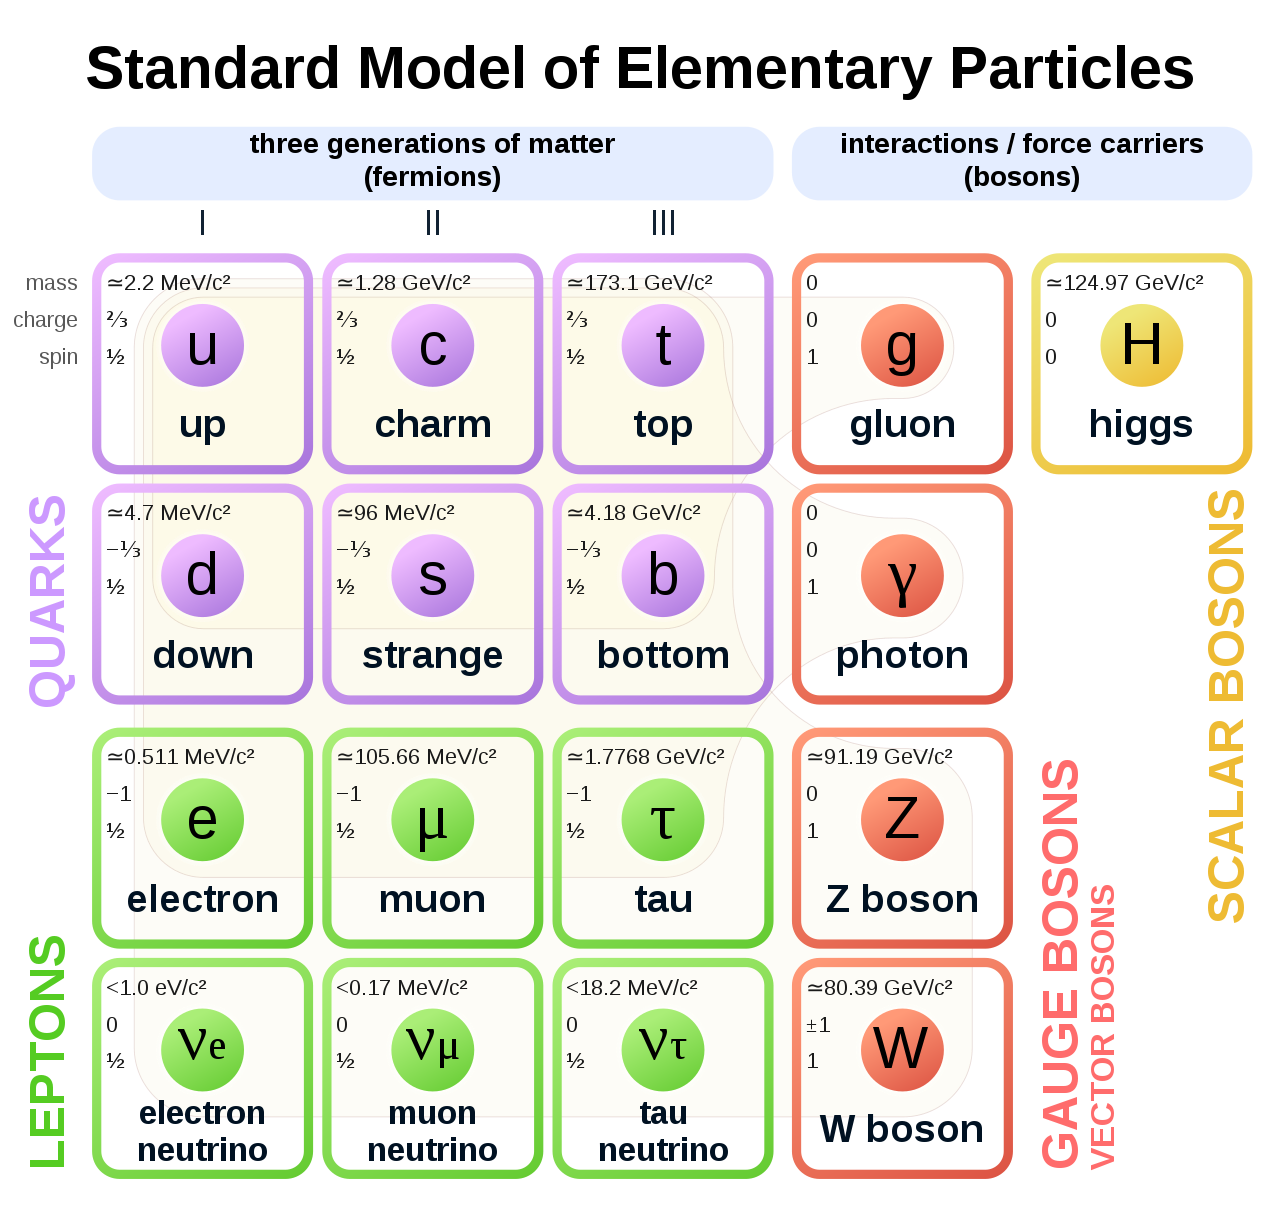
\includegraphics[width=0.75\textwidth]{figuresTHE/SM1.png}
  \end{center}
  \caption{ 标准模型中的基本粒子。图中还显示了各个粒子的质量、电荷和自旋。}
    \label{fig:SM1}
\end{figure}

\subsection{量子电动力学}
\label{sec:QED}
量子电动力学(Quantum electrodynamics, QED)是量子场论中最为成功的理论之一,
它描述了带电粒子之间的电磁相互作用,是一个阿贝尔规范理论~\cite{GAUGE1},
建立在对称群$U(1)$之上,规范场即为电磁场。
对于一个自由的狄拉克费米子$\psi(x)$,其拉氏量$\mathcal{L}_0$为:
\begin{equation} 
\label{eq:QED1}
\mathcal{L}_0= i \bar{\psi}(x) \gamma^{\mu} \partial_{\mu} \psi(x) - m \bar{\psi}(x) \psi(x)
\end{equation}
它在全局$U(1)$对称变换下是不变的:
\begin{equation} 
\label{eq:QED2}
\psi(x) \rightarrow (\psi(x))' = exp\{  i\theta \} \psi(x)
\end{equation}
其中$exp\{  i\theta \} \psi(x)$是$U(1)$的表示,$\theta$为任意实数常数,当重新定义这个变换使它依赖于时空坐标$\theta=\theta(x)$,即局部$U(1)$规范变换,
则破坏了拉氏量$\mathcal{L}_0$的不变性:
\begin{equation} 
\label{eq:QED3}
\partial_{\mu} \psi(x)  \rightarrow exp\{  i\theta(x) \} (\partial_{\mu} + i\partial_{\mu}\theta(x) ) \psi(x)
\end{equation}
规范原理要求拉氏量$\mathcal{L}_0$此时仍然保持不变性,
则需要引入一个自旋为1的矢量场$A_{\mu}(x)$,即电磁场,来抵消上述第二项,它服从变换:
\begin{equation} 
\label{eq:QED4}
A_{\mu}(x) \rightarrow A'_{\mu}(x) = A_{\mu}(x)- \frac{1}{e} \partial_{\mu}\theta(x)
\end{equation}
其中e是耦合常数,由此在偏微分基础上定义协变微分$D_{\mu}$:
\begin{equation} 
\label{eq:QED5}
D_{\mu}\psi(x) \equiv \left[ \partial_{\mu}+ieA_{\mu}(x) \right] \psi(x)
\end{equation}
它的变换可以与费米场的变换相互抵消:
\begin{equation} 
\label{eq:QED6}
D_{\mu}\psi(x) \rightarrow (D_{\mu}\psi)'(x)= exp\{  i\theta(x) \} D_{\mu}\psi(x)
\end{equation}
另外矢量场$A_{\mu}(x)$的自由拉氏量$\mathcal{L}_1$是:
\begin{equation} 
\label{eq:QED7}
\mathcal{L}_1=-\frac{1}{4}F_{\mu\nu}(x)F^{\mu\nu}(x)
\end{equation}
结合上述,可以得到最终的QED拉氏量$\mathcal{L}_{QED}$:
%\begin{equation} 
%\label{eq:QED8}
 %\begin{aligned}
 % \mathcal{L}_{QED} = i \bar{\psi}(x) \gamma^{\mu} D_{\mu} \psi(x) - m \bar{\psi}(x) \psi(x) + \mathcal{L}_1
  %\\
 % = i \bar{\psi}(x) \gamma^{\mu} \partial_{\mu} \psi(x) - m \bar{\psi}(x) \psi(x) - e A_{\mu}(x) 
  %\bar{\psi}(x) \gamma^{\mu} \psi(x) - -\frac{1}{4}F_{\mu\nu}(x)F^{\mu\nu}(x)
 %\end{aligned}
%\end{equation}
\begin{equation}
\label{eq:QED8}
\begin{split}
\mathcal{L}_{QED} & =i \bar{\psi}(x) \gamma^{\mu} D_{\mu} \psi(x) - m \bar{\psi}(x) \psi(x) + \mathcal{L}_1\\
& = i \bar{\psi}(x) \gamma^{\mu} \partial_{\mu} \psi(x) - m \bar{\psi}(x) \psi(x) \\
&\quad - e A_{\mu}(x)\bar{\psi}(x) \gamma^{\mu} \psi(x) - -\frac{1}{4}F_{\mu\nu}(x)F^{\mu\nu}(x)
\end{split}
\end{equation}
它在局部$U(1)$规范变换下保持不变,
其中第一项和第二项是狄拉克费米子场的自由拉氏量;
%将在后续介绍希格斯玻色子之后重新给出;
第三项是带电费米子与电磁场的电磁相互作用项;
第四项是电磁场的动能项,
由于电磁场的质量项$\frac{1}{2}m^2A^{\mu}A_{\mu}$在局部规范变换下不具有不变性,
因此光子没有质量。



\subsection{量子色动力学}
\label{sec:QCD}
量子色动力学(Quantum chromodynamics, QCD)是描述由胶子g作为媒介子的夸克之间强相互作用的理论,
它是一个非阿贝尔规范理论~\cite{SM0},建立在局部规范对称群$SU(3)$的基础上。
对于夸克场$q_f^{\alpha}$,其中$\alpha$是色荷指标,$f$为夸克的味指标,体系自由拉氏量$\mathcal{L}_0$为:
\begin{equation} 
\label{eq:QCD1}
\mathcal{L}_0=\sum_f \bar{q}_f (i\gamma^{\mu}\partial_{\mu}-m_f)q_f
\end{equation}
其在色荷空间中任意的全局对称变换$SU(3)$下是不变的:
\begin{equation} 
\label{eq:QCD2}
 \begin{split}
 &  q_f^{\alpha} \rightarrow (q_f^{\alpha})'=U^{\alpha}_{~\beta}q_f^{\beta}  \\
 & UU^{\dagger} =U^{\dagger}U=1, \quad det~U=1
 \end{split}
\end{equation}
其中$U$是$SU(3)$的矩阵表示,可以写成如下形式:
\begin{equation} 
\label{eq:QCD3}
U=exp\Bigg\{ i\frac{\lambda^{a}}{2}\theta_a \Bigg\} 
\end{equation}
这里$\frac{\lambda^{a}}{2}(a=1,2,\dots,8)$是李代数$SU(3)$基础表示中的八个生成元,$\theta_a$是任意参数。
生成元$\frac{\lambda^{a}}{2}$之间满足如下代数关系:
\begin{equation} 
\label{eq:QCD4}
\left[ \frac{\lambda^{a}}{2}, \frac{\lambda^{b}}{2} \right]=if^{abc}\frac{\lambda^{c}}{2}
\end{equation}
其中$f^{abc}$是李代数$SU(3)$的结构参数。

类似量子电动力学,当要求自由拉氏量$\mathcal{L}_0$在$SU(3)$局部规范变换下保持不变:
\begin{equation} 
\label{eq:QCD5}
U(x)=exp\Bigg\{ i\frac{\lambda^{a}}{2}\theta_a(x) \Bigg\} 
\end{equation}
由于$U(x)$包含八个独立的规范参数,需要将偏微分$\partial_{\mu}$换成协变微分$D_{\mu}$并引入八个独立的规范场以保证拉氏量$\mathcal{L}_0$的不变性:
\begin{equation} 
\label{eq:QCD6}
D^{\mu}q_f=\left[   \partial^{\mu}+ig_s\frac{\lambda^{a}}{2}G^{\mu}_a(x)  \right] q_f \equiv
\left[   \partial^{\mu}+ig_sG^{\mu}(x) \right] q_f
\end{equation}
其中$g_s$为耦合常数,八个规范场$G^{\mu}_a(x)$即对应于八个不同的规范玻色子,胶子。
这里引入了一个缩写表示:
\begin{equation} 
\label{eq:QCD7}
\left[G^{\mu}(x)\right]_{\alpha\beta} \equiv \left( \frac{\lambda^{a}}{2} \right)_{\alpha\beta}G^{\mu}_a(x) 
\end{equation}
当要求协变微分项$D^{\mu} q_f$与色荷矢量$q_f$以完全相同的方式进行变换,可以得到规范场$G^{\mu}$的变换属性:
\begin{equation} 
\label{eq:QCD8}
D^{\mu} \rightarrow (D^{\mu})' = UD^{\mu}U^{\dagger}, \quad 
G^{\mu} \rightarrow (G^{\mu})'=UG^{\mu}U^{\dagger}+\frac{i}{g_s}(\partial^{\mu}U)U^{\dagger}
\end{equation}
由此,在$SU(3)$局部规范变换下有:
\begin{equation} 
\label{eq:QCD9}
 \begin{split}
  & q_f^{\alpha}\rightarrow (q_f^{\alpha})'=q_f^{\alpha}+i\left( \frac{\lambda^{a}}{2} \right)_{\alpha\beta}\delta\theta_a q_f^{\beta}
   \\
  & G^{\mu}_a\rightarrow (G^{\mu}_a)'=G^{\mu}_a-\frac{1}{g_s}\partial^{\mu}\left(\delta\theta_a\right)-f^{abc}\delta\theta_bG^{\mu}_c
  \end{split}
\end{equation}
由于李代数$SU(3)$的非交换性,使得QCD中规范场的规范变换比QED中规范场光子的变换要复杂很多,
拉氏量中会出现了涉及胶子场自身的附加项,
并且带有不同色荷的夸克都以完全相同的耦合强度$g_s$与胶子场耦合。

为了构建胶子场的动力学,引入相应的场强$G^{\mu\nu}(x)$:
\begin{equation} 
\label{eq:QCD10}
 \begin{split}
  & G^{\mu\nu}(x) \equiv -\frac{i}{g_s}\left[D^{\mu},D^{\nu} \right] = \partial^{\mu}G^{\nu}-\partial^{\nu}G^{\mu} +i g_s\left[G^{\mu},G^{\nu} \right]
   \equiv \frac{\lambda^{a}}{2}G^{\mu\nu}_a(x)
   \\
&   G^{\mu\nu}_a(x)= \partial^{\mu}G^{\nu}_a-\partial^{\nu}G^{\mu}_a -g_sf^{abc}G^{\mu}_bG^{\nu}_c 
 \end{split}
\end{equation}
在$SU(3)$规范变化下有:
\begin{equation} 
\label{eq:QCD11}
G^{\mu\nu} \rightarrow  (G^{\mu\nu})'=UG^{\mu\nu}U^{\dagger}
\end{equation}
并且$\frac{1}{2}G^{\mu\nu}_a G^a_{\mu\nu}=Tr(G^{\mu\nu}G_{\mu\nu})$是不变的,
最终可以得到完整的$SU(3)$局部规范不变的QCD拉氏量:
\begin{equation} 
\label{eq:QCD12}
\mathcal{L}_{QCD}  \equiv  -\frac{1}{4}G^{\mu\nu}_a G_{\mu\nu}^a +\sum_f \bar{q}_f (i\gamma^{\mu}D_{\mu}-m_f)q_f
\end{equation}
由式~\ref{eq:QCD8}~可知胶子场的质量项$\frac{1}{2}m^2_G G^{\mu}_a G^a_{\mu}$在$SU(3)$规范变换下不是不变的,
因此它不会出现在拉氏量$\mathcal{L}_{QCD}$中,
这表明胶子是无质量的规范玻色子。

将拉氏量$\mathcal{L}_{QCD}$展开之后:
\begin{equation} 
\label{eq:QCD13}
 \begin{split}
   \mathcal{L}_{QCD}  \quad = \quad & -\frac{1}{4} (\partial^{\mu}G^{\nu}_a-\partial^{\nu}G^{\mu}_a) (\partial_{\mu}G_{\nu}^a-\partial_{\nu}G_{\mu}^a)+
   \sum_f \bar{q}^{\alpha}_f (i\gamma^{\mu}\partial_{\mu}-m_f)q^{\alpha}_f
   \\
  & -g_s G^{\mu}_a \sum_f \bar{q}^{\alpha}_f \gamma^{\mu} \left( \frac{\lambda^{a}}{2} \right)_{\alpha\beta} q^{\beta}_f
   \\
  & +\frac{g_s}{2} f^{abc} (\partial^{\mu}G^{\nu}_a-\partial^{\nu}G^{\mu}_a) G^b_{\mu} G^c_{\nu} 
   -\frac{g_s^2}{4} f^{abc} f_{ade} G_b^{\mu} G_c^{\nu}  G^d_{\mu} G^e_{\nu} 
 \end{split}
\end{equation}
其中第一行第一项是胶子的动能项,
第二项是夸克场的自由拉氏量;
%,将在后续介绍希格斯玻色子之后重新给出;
第二行是夸克和胶子之间的耦合项;
第三行是胶子的自相互作用项,包括三个胶子耦合和四个胶子耦合。
伴随着$SU(3)$规范群的特殊性,使得QCD还有一些独特的性质比如渐近自由~\cite{ASF1,ASF2}和色禁闭~\cite{CONF},
渐近自由是指在能量较高时,夸克之间的强相互作用很弱,而在低能情况下,相互作用变强;
色禁闭指带有色荷的夸克或胶子不能单独存在,它们只能通过结合形成不带色荷的强子。

\subsection{电弱理论}
\label{sec:EW}

为了描述弱相互作用,需要更精细的结构。
手征是基本粒子的一个属性,它是$\gamma^5\equiv i \gamma^0\gamma^1\gamma^2\gamma^3$的本征态,按本征值不同可以分为左手和右手,
左手费米子和右手费米子在弱相互作用中有着不同的性质,
并且弱相互作用的规范理论需要结合电磁相互作用的规范理论一起描述,称为电弱理论(Electroweak theory, EW)~\cite{SM2},
首先,考虑如下对称性:
\begin{equation} 
\label{eq:EW1}
G \equiv SU(2) \otimes U(1)
\end{equation}
为了简便起见,这里仅考虑第一代夸克$~(u, d)~$和轻子$~(\nu_e, e^-)~$,其他代情形类似,
对于第一代夸克$~(u, d)~$,用L表示左手场,R表示右手场,引入如下记号:
\begin{equation} 
\label{eq:EW2}
\psi_1(x)=  \left( \begin{array}{l}  u \\  d \end{array} \right) _L, \quad  \psi_2(x)=u_R, \quad \psi_3 = d_R 
\end{equation}
同样对于第一代轻子$~(\nu_e, e^-)~$,有如下表示:
\begin{equation} 
\label{eq:EW3}
\psi_1(x)=  \left( \begin{array}{l}  \nu_e \\  e^- \end{array} \right) _L, \quad  \psi_2(x)=\nu_{eR}, \quad \psi_3 = e^-_R 
\end{equation}
由此,体系的自由拉氏量$\mathcal{L}_0$可表示成:
\begin{equation} 
\label{eq:EW4}
\mathcal{L}_0= i\bar{u}(x)\gamma^{\mu}\partial_{\mu}u(x)+i\bar{d}(x)\gamma^{\mu}\partial_{\mu}d(x)
=\sum_{j=1}^3 i\bar{\psi}_j(x)\gamma^{\mu}\partial_{\mu}\psi_j(x)
\end{equation}
它在味空间的全局对称变换G下是不变的:
\begin{equation} 
\label{eq:EW5}
 \begin{split}
  &\psi_1(x) \rightarrow \psi'_1(x)= exp\{iy_1\beta\}U_L\psi_1(x)
  \\
&  \psi_2(x) \rightarrow \psi'_2(x)= exp\{iy_2\beta\}\psi_2(x)
  \\
&  \psi_3(x) \rightarrow \psi'_3(x)= exp\{iy_3\beta\}\psi_3(x)
 \end{split}
\end{equation}
其中$SU(2)$的表示有如下形式:
\begin{equation} 
\label{eq:EW6}
U_L=exp\left\{ i\frac{\sigma_i}{2}\alpha^i \right\} \quad (i=1,2,3)
\end{equation}
$\sigma_i$为泡利矩阵,$U_L$仅作用在双重态$\psi_1$上。
参数$y_i$被称为超荷,是与对称性G相关的一个守恒荷。
式~\ref{eq:EW4}~中没有引入质量项,因为它会破坏整体的对称性,
质量项将在后面介绍希格斯机制之后给出。

同QED和QCD,当要求拉氏量$\mathcal{L}_0$满足$SU(2) \otimes U(1)$局部规范不变性,
即令$\alpha^i=\alpha^i(x)$和$\beta=\beta(x)$,
需要用协变微分$D_{\mu}$代替偏微分$\partial_{\mu}$,因为有四个规范参数$\alpha^i(x)$和$\beta(x)$,
这里引入四个规范场$W^i_{\mu}(x)$和$B_{\mu}(x)$:
\begin{equation} 
\label{eq:EW7}
 \begin{split}
  &D_{\mu}\psi_1(x) \equiv \left[ \partial_{\mu}+ig\widetilde{W}_{\mu}(x)+ig'y_1B_{\mu}(x) \right] \psi_1(1)
  \\
 & D_{\mu}\psi_2(x) \equiv \left[ \partial_{\mu}+ig'y_2B_{\mu}(x) \right] \psi_2(x)
  \\
 & D_{\mu}\psi_3(x) \equiv \left[ \partial_{\mu}+ig'y_3B_{\mu}(x) \right] \psi_3(x)
 \end{split}
\end{equation}
其中:
\begin{equation} 
\label{eq:EW8}
\widetilde{W}_{\mu}(x) \equiv \frac{\sigma_i}{2} W^i_{\mu}(x)
\end{equation}
$g$和$g'$是耦合常数,到此,有了四个规范场用来构建四个玻色子$W^{\pm}$、$Z$和$\gamma$。
当要求协变微分项$D_{\mu}\psi_j(x)$与$\psi_j(x)$以相同的方式进行变换,可以得到规范场$B_{\mu}(x)$和$\widetilde{W}_{\mu}(x)$的变换方式:
\begin{equation} 
\label{eq:EW9}
 \begin{split}
 & B_{\mu}(x) \rightarrow B'_{\mu}(x)=  B_{\mu}(x)-  \frac{1}{g'} \partial_{\mu}\beta(x)
  \\
 & \widetilde{W}_{\mu}(x) \rightarrow  \widetilde{W}'_{\mu}(x)=   U_L(x)\widetilde{W}_{\mu}(x) U^{\dagger}_L(x)+\frac{i}{g} \partial_{\mu}U_L(x) U^{\dagger}_L(x)
 \end{split}
\end{equation}
其中:
\begin{equation} 
\label{eq:EW19}
U_L(x)=exp\left\{ i\frac{\sigma_i}{2}\alpha^i(x) \right\} \quad (i=1,2,3)
\end{equation}
可以看到$B_{\mu}$的变换方式与QED中电磁场的变换方式相同,
而对应于$SU(2)$的场$W^i_{\mu}$的变换方式与QCD中胶子场的变换方式类似。

因此,可以得到在$SU(2) \otimes U(1)$局部规范变换下不变的拉氏量$\mathcal{L}_1$:
\begin{equation} 
\label{eq:EW10}
\mathcal{L}_1= \sum_{j=1}^3 i\bar{\psi}_j(x)\gamma^{\mu}D_{\mu}\psi_j(x)
\end{equation}
接下来是构建协变的规范场动能项:
\begin{equation} 
\label{eq:EW11}
 \begin{split}
 & B_{\mu\nu}= \partial_{\mu}B_{\nu}- \partial_{\nu}B_{\mu}
  \\
 & \widetilde{W}_{\mu\nu} \equiv -\frac{i}{g} \left[ \left(  \partial_{\mu}+ig\widetilde{W}_{\mu} \right) ,  \left(  \partial_{\nu}+ig\widetilde{W}_{\nu}  \right)    \right]
  =\partial_{\mu}\widetilde{W}_{\nu}- \partial_{\nu}\widetilde{W}_{\mu}+ ig \left[  \widetilde{W}_{\mu}  ,\widetilde{W}_{\nu}   \right]
 \end{split}
\end{equation}
其中:
\begin{equation} 
\label{eq:EW12}
\widetilde{W}_{\mu\nu} \equiv \frac{\sigma_i}{2} W^i_{\mu\nu}, \quad 
W^i_{\mu\nu}= \partial_{\mu}W^i_{\nu}- \partial_{\nu}W^i_{\mu}- g\epsilon^{ijk}W^j_{\mu}W^k_{\nu}
\end{equation}
这里$B_{\mu\nu}$在变换下是不变的,而$\widetilde{W}_{\mu\nu}$是协变的:
\begin{equation} 
\label{eq:EW13}
B_{\mu\nu} \rightarrow B_{\mu\nu}, \quad \widetilde{W}_{\mu\nu}  \rightarrow   U_L \widetilde{W}_{\mu\nu} U^{\dagger}_L
\end{equation}
最后,得到的在$SU(2) \otimes U(1)$局部规范变换下不变的完整EW拉氏量$\mathcal{L}_{EW}$可以表示成:
\begin{equation} 
\label{eq:EW14}
 \begin{split}
  \mathcal{L}_{EW}&= \mathcal{L}_1 - \frac{1}{4}B_{\mu\nu}B^{\mu\nu}-\frac{1}{2}Tr\left[ \widetilde{W}_{\mu\nu}\widetilde{W}^{\mu\nu} \right]
  \\
 & =\sum_{j=1}^3 i\bar{\psi}_j(x)\gamma^{\mu}D_{\mu}\psi_j(x) - \frac{1}{4}B_{\mu\nu}B^{\mu\nu}-\frac{1}{4}W_{\mu\nu}W^{\mu\nu}
 \end{split}
\end{equation}
其中电磁场$A_{\mu}$和弱相互作用中的中性流$Z^0$是场$B_{\mu}$和场$W^3_{\mu}$的混合:
\begin{equation} 
\label{eq:EW15}
 \left( \begin{array}{l} A_{\mu}  \\  Z^0_{\mu} \end{array} \right) = 
 \left( \begin{array}{l}  \cos \theta_W \quad \sin \theta_W \\  - \sin \theta_W  \quad \cos \theta_W \end{array} \right) 
 \left( \begin{array}{l}  B_{\mu} \\  W^3_{\mu} \end{array} \right) 
\end{equation}
玻色子场$W^{\pm}$是$W^1$和$W^2$的线性组合:
\begin{equation} 
\label{eq:EW16}
W^{\pm}=\frac{1}{\sqrt{2}}\left(   W^1 \mp iW^2  \right)
\end{equation}
并且式~\ref{eq:EW15}~中参数$\theta_W$与式~\ref{eq:EW7}~中耦合参数$g$、$g'$和QED中耦合参数e有如下关系:
\begin{equation} 
\label{eq:EW17}
g \sin \theta_W = g' \cos \theta_W \equiv e
\end{equation}
EW拉氏量~\ref{eq:EW14}~中第一项是费米子与四个玻色子场$W^{\pm}$、$Z$和$\gamma$的相互作用项,
后两项描述的是四个玻色子场的自相互作用,包含三顶点和四顶点自相互作用。
体系的规范对称性要求费米子场和玻色子场都是无质量的,
需要引入对称性破缺和希格斯机制赋予它们相应的质量,将在第~\ref{sec:SSB}~小节介绍。
其中三代夸克的弱相互作用本征态$d'$、$s'$、$b'$并不是它们的质量本征态d、s、b,
它们之间是通过一个的酉矩阵V,称为CKM矩阵~\cite{CKM}联系起来的:
\begin{equation} 
\label{eq:EW18}
 \left( \begin{array}{l} d' \\  s' \\ b' \end{array} \right) = V
 \left( \begin{array}{l} d \\  s \\ b \end{array} \right), \quad VV^{\dagger}=V^{\dagger}V=1
\end{equation}
而且电弱相互作用也有一些特殊的性质,
比如味守恒、只有左手费米子和右手反费米子能通过$W^{\pm}$玻色子耦合等。

\subsection{对称性自发破缺}
\label{sec:SSB}

在规范原理的基础上,电弱理论很好的描述了电磁相互作用和弱相互作用,也包含了规范玻色子的自相互作用项,
这是由对称群的非交换性引起的,规范对称性也保证了拉氏量的可重整性。
但是,在这个理论框架下,四种规范玻色子都是无质量的粒子,对于光子来说确实如此,
但是实验上观测到的$W^{\pm}$和$Z$玻色子都是大质量粒子,
为了赋予它们质量,在保证拉氏量的整体对称性的同时,
需要以某种方式破坏其对称性,即对称性自发破缺(Spontaneous symmetry breaking, SSB)~\cite{SM4,SM5,SM6}。
考虑一个复标量场$\phi(x)$,其拉氏量$\mathcal{L}_0$为:
\begin{equation} 
\label{eq:SSB1}
\mathcal{L}_0= \partial_{\mu} \phi^{\dagger} \partial^{\mu} \phi - V(\phi), \quad
V(\phi)=\mu^2 \phi^{\dagger} \phi + h \left(  \phi^{\dagger} \phi   \right)^2
\end{equation}
它在全局$U(1)$对称变换下具有不变性:
\begin{equation} 
\label{eq:SSB2}
\phi(x)  \rightarrow \phi'(x)= exp\{ i\theta \}\phi(x)
\end{equation}

为了确保基态存在,参数h需满足$h>0$。
对于二次项$\mu^2 \phi^{\dagger} \phi$,如图~\ref{fig:SSB1}~所示,有两种可能:
当$\mu^2>0$时,势能项$V(\phi)$在$\phi=0$时有平凡的最小值,
它描述的是一个质量为$\mu$并具有四顶点自相互作用的标量粒子;
当$\mu^2<0$时,势能项$V(\phi)$在如下条件下有极小值:
\begin{equation} 
\label{eq:SSB3}
|\phi_0|= \sqrt{\frac{-\mu^2}{2h}} \equiv \frac{v}{\sqrt{2}} >0 , \quad V(\phi_0)=-\frac{h}{4}v^4
\end{equation}
由于拉氏量具有$U(1)$对称性,体系具有无穷多个简并基态:
\begin{equation} 
\label{eq:SSB4}
\phi_0(x)=\frac{v}{\sqrt{2}}exp\left\{ i\theta\right\}
\end{equation}
当选择一个特定的解作为基态,体系的对称性自发的被破坏了,
如果将激发态在基态的基础上参数化:
\begin{equation} 
\label{eq:SSB5}
\phi(x) \equiv \frac{1}{\sqrt{2}}\left[ v+ \varphi_1(x) + i	\varphi_2(x) \right]
\end{equation}
其中$\varphi_1$和$\varphi_2$是实标量场,势能项$V(x)$可以化为如下形式:
\begin{equation} 
\label{eq:SSB6}
V(\phi)=V(\phi_0)- \mu^2 \varphi^2+ hv\varphi_1(\varphi^2_1+ \varphi^2_2)+ \frac{h}{4}(\varphi^2_1+ \varphi^2_2)^2
\end{equation}
这里,实标量场$\varphi_1$是有质量的$m_{\varphi_1}^2=-2\mu^2$,场$\varphi_2$是无质量的。

\begin{figure}
  \begin{center}
    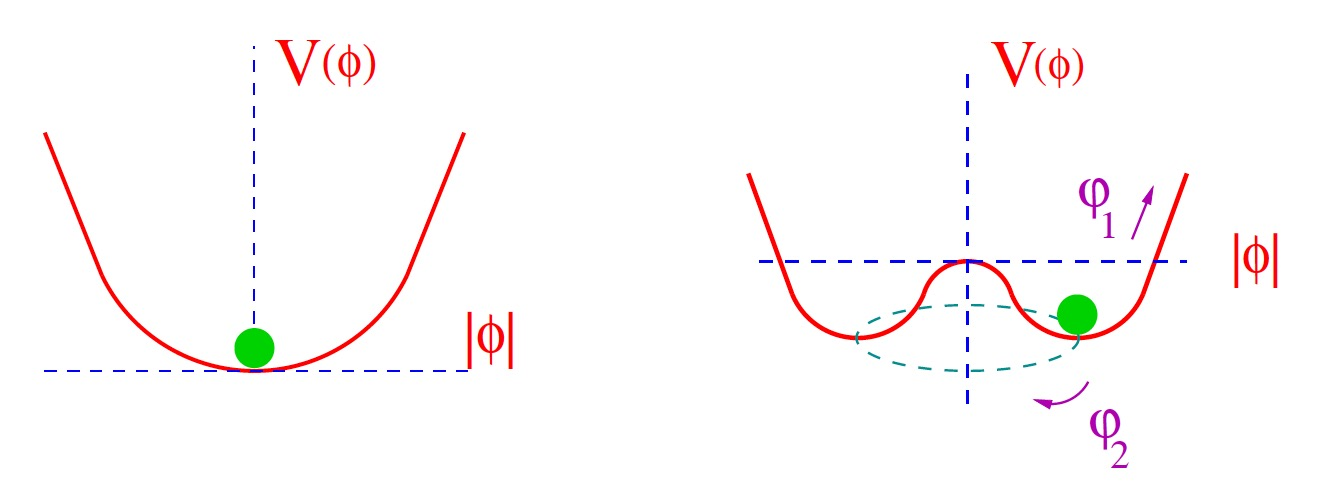
\includegraphics[width=0.85\textwidth]{figuresTHE/SSB.jpg}
  \end{center}
  \caption{
对称性自发破缺。
}
    \label{fig:SSB1}
\end{figure}


第一种可能$\mu^2>0$是仅具有单个基态的简单情形。
第二种情形$\mu^2<0$即对称性自发破缺,
过程中会出现一个无质量的粒子$\varphi_2$。
对称性自发破缺是物理系统的对称性自发破坏的过程,
它可以描述那些体系拉氏量的对称性和体系基态对称性不一致的物理系统。
无质量粒子的出现是一个与对称性自发破缺机制相关的一般性结果,
称为Goldstone定理:如果体系拉氏量在连续对称变换G作用下是不变的,
但是基态仅在G的子群H的作用下才具有不变性,
那么体系会存在与破缺的对称性相对应的多个无质量的Goldstone玻色子,
玻色子的个数等于G的生成元个数减去H的生成元个数。

\subsubsection{$W^{\pm}$和$Z$玻色子质量}
\label{sec:SSBWZ}
在第二种情况$\mu^2<0$下,对于拉氏量~\ref{eq:SSB1}~,当考虑一个$SU(2)$双重态的复标量场:
\begin{equation} 
\label{eq:SSB7}
\phi(x) \equiv 
 \left( \begin{array}{l} \phi^{(+)}(x) \\  \phi^{(0)}(x) \end{array} \right)
\end{equation}
类似电弱理论,利用规范原理构建一个在$SU(2)\otimes U(1)$局部规范变换下具有不变性的拉氏量$\mathcal{L}_S$:
\begin{equation} 
\label{eq:SSB8}
\begin{split}
& \mathcal{L}_S= (D_{\mu}\phi)^{\dagger}D_{\mu}\phi- \mu^2 \phi^{\dagger} \phi - h \left(  \phi^{\dagger} \phi   \right)^2 \quad (h>0, \mu^2<0)
%\end{equation}
%\begin{equation} 
%\label{eq:SSB9}
\\
&D^{\mu}\phi= \left[ \partial^{\mu}+ig\widetilde{W}^{\mu}(x)+ig'y_{\phi}B^{\mu}(x) \right] \psi_1(1), \quad y_{\phi}=\frac{1}{2}
\end{split}
\end{equation}
根据标量场$\phi(x)$与电磁场$A^{\mu}(x)$的耦合情况,即场$\phi^{(0)}(x)$不带电荷,场$\phi^{(+)}(x)$带有正电荷,
可以确定标量场的超荷$y_{\phi}$。
其中势能项与式~\ref{eq:SSB1}~类似,
体系具有无穷多个简并基态,满足:
\begin{equation} 
\label{eq:SSB10}
|\langle 0| \phi^{(0)} |0\rangle|=\sqrt{\frac{-\mu^2}{2h}}  \equiv \frac{v}{\sqrt{2}}
\end{equation}
因为电荷是守恒荷,只有中性标量场$\phi^{(0)}$才能获得真空期望值。
当体系处于某个特定的基态,
$SU(2)\otimes U(1)$规范对称性会自发的破缺到电磁相互作用的$U(1)$规范对称性,
根据Goldstone定理,会出现三个无质量的Goldstone玻色子。

当用四个实场$\theta^i(x)$和$H(x)$和基态来一般性的表示双重态的复标量场$\phi(x)$:
\begin{equation} 
\label{eq:SSB11}
\phi(x)=exp\left\{  i \frac{\sigma_i}{2}\theta^i(x)  \right\} \frac{1}{\sqrt{2}}
\left( \begin{array}{l} 0 \\  v+H(x) \end{array} \right)
\end{equation}
这样表示的目的是利用拉氏量的$SU(2)$局部规范对称性来消除对$\theta^i(x)$的依赖性,
%这样表示的目的在于拉氏量的$SU(2)$局部规范对称性可以消除对$\theta^i(x)$的依赖性,
这三个场就是与对称性自发破缺机制相关联的三个无质量的Goldstone玻色子场。
协变微分项~\ref{eq:SSB8}~中包含标量场和$SU(2)\otimes U(1)$规范玻色子的耦合,
当选取物理的规范,即单位规范令$\theta^i(x)=0$,并结合式~\ref{eq:EW15}~,标量场拉氏量~\ref{eq:SSB8}~的动能项可以化为:
\begin{equation} 
\label{eq:SSB12}
(D_{\mu}\phi)^{\dagger}D_{\mu}\phi \xrightarrow{\theta^i=0} \frac{1}{2} \partial_{\mu}H \partial^{\mu}H
+(v+H)^2\left\{    \frac{g^2}{4}W^{\dagger}_{\mu}W^{\mu} +\frac{g^2}{8\cos^2 \theta_W}Z_{\mu}Z^{\mu}    \right\}
\end{equation}
中性标量场$H(x)$为$W^{\pm}$和$Z$玻色子分别提供了一个二次项,即这三个规范玻色子有了质量:
\begin{equation} 
\label{eq:SSB13}
M_Z \cos \theta_W=M_W=\frac{1}{2}vg
\end{equation}
到此,可以看到对称性自发破缺机制怎样巧妙的为弱相互作用的中间玻色子$W^{\pm}$和$Z$赋予质量。
当要求拉氏量$\mathcal{L}_S$满足$SU(2)\otimes U(1)$局部规范对称,可以保证相应量子场论的可重整性,
引入对称性自发破缺机制之后,三个无质量的Goldstone玻色子会伴随着破缺的对称性而出现,
由于体系已有的规范对称性,可以通过选取单位规范将它们安全的从拉氏量中移除,
从而$W^{\pm}$和$Z$玻色子成功获得了质量。

\subsubsection{标量玻色子}
\label{sec:SSBH}

拉氏量~\ref{eq:SSB8}~中引入对称性自发破缺机制后,模型中出现了一个新的标量玻色子:希格斯玻色子$H$。
在单位规范下,拉氏量$\mathcal{L}_S$可以化简为如下形式:
\begin{equation} 
\label{eq:SSB14}
\mathcal{L}_S=\frac{1}{4}hv^4+\mathcal{L}_H+\mathcal{L}_{HG}
\end{equation}
其中:
\begin{equation} 
\label{eq:SSB15}
\mathcal{L}_H=\frac{1}{2}\partial_{\mu}H\partial^{\mu}H -\frac{1}{2}M_H^2 H^2
-\frac{M_H^2 }{2v}H^3 -\frac{M_H^2 }{8v^2}H^4
\end{equation}
\begin{equation} 
\label{eq:SSB16}
\mathcal{L}_{HG}= \left( 1+\frac{H}{v} \right)^2 M_W^2 W^{\dagger}_{\mu}W^{\mu} 
+ \frac{1}{2} \left( 1+\frac{H}{v} \right)^2 M_Z^2 Z_{\mu}Z^{\mu} 
\end{equation}
并且$H$玻色子具有质量:
\begin{equation} 
\label{eq:SSB17}
M_H=\sqrt{-2\mu^2}=\sqrt{2h}v
\end{equation}
式~\ref{eq:SSB16}~中希格斯玻色子的相互作用项有一个典型的特征:
它们总是与耦合在一起的玻色子的质量的平方成正比,由$M_H$,$M_W$,$M_Z$和真空期望值$v/\sqrt{2}$决定。


\subsubsection{费米子质量}
\label{sec:SSBF}

由于规范对称性的要求,费米子质量项:
\begin{equation} 
\label{eq:SSB18}
\mathcal{L}_F=-m\bar{\phi}\phi=-m(\bar{\phi}_L\phi_R+\bar{\phi}_R\phi_L)
\end{equation}
是不允许存在的。但是,由于在模型中已经引入了新的双重态复标量场,
于是可以构建如下规范对称的费米子-标量场耦合项,也称为Yukawa耦合:
\begin{equation} 
\label{eq:SSB19}
\begin{split}
\mathcal{L}_Y= & -c_1 (\bar{u},\bar{d})_L 
\left( \begin{array}{l} \phi^{(+)} \\  \phi^{(0)} \end{array} \right) d_R
-c_2 (\bar{u},\bar{d})_L 
\left( \begin{array}{l} \phi^{(0)\ast} \\  -\phi^{(-)} \end{array} \right) u_R
\\
& -c_3 (\bar{\nu}_e,\bar{e})_L 
\left( \begin{array}{l} \phi^{(+)} \\  \phi^{(0)} \end{array} \right) e_R
+ h.c.
\end{split}
\end{equation}
其中第二项涉及标量场的电荷共轭项$\phi^c \equiv i\sigma_2 \phi^*$,
引入对称性自发破缺并选取单位规范之后,
上述Yukawa耦合的拉氏量可以化简为:
\begin{equation} 
\label{eq:SSB20}
\mathcal{L}_Y=
-\frac{1}{\sqrt{2}}(v+H)\left(  c_1\bar{d}d+ c_2\bar{u}u +c_3\bar{e}e  \right)
\end{equation}
因此,费米子在对称性自发破缺机制下也获得了质量:
\begin{equation} 
\label{eq:SSB21}
m_d=c_1\frac{v}{\sqrt{2}}, \quad 
m_u=c_2\frac{v}{\sqrt{2}}, \quad 
m_e=c_3\frac{v}{\sqrt{2}}
\end{equation}
其中$c_i$为任意常数,用质量项表示拉氏量得:
\begin{equation} 
\label{eq:SSB22}
\mathcal{L}_Y=
-(1+\frac{H}{v})\left(  m_d\bar{d}d+ m_u\bar{u}u +m_e\bar{e}e  \right)
\end{equation}
可以看到轻子和夸克质量在标准模型中是自由参数,
而且费米子与希格斯玻色子之间的耦合强度与费米子质量成正比。
%但是其中未包含中微子质量项,因为实验上并未观测到希格斯玻色子与中微子有明显耦合的现象。


\section{希格斯玻色子}
\label{sec:Higgs}

对称性自发破缺机制中的关键标量玻色子,希格斯玻色子的寻找已经在粒子物理领域持续了数十年。
理论提出来之后二十多年,
CERN的大型正负电子对撞机和Tevatron的正负强子对撞机先后对希格斯玻色子质量的给出严格的区间限制~\cite{TEVN,LEP},
在2010年,LHC以比之前更高的质心能量和总积分亮度开始取数,将会在第~\ref{cha:EXP}~章介绍LHC,
最后在2012年,LHC上的两个大型探测器ATLAS和CMS(The Compact Muon Solenoid)终于发现了一个与标准模型中希格斯玻色子相符合的粒子~\cite{ATLASHIGGS,CMSHIGGS},
其质量在大约125GeV左右,
这是粒子物理学史上一个重大的里程碑。
在发现希格斯玻色子之后,接下来实验上非常重要的一个任务便是
对希格斯玻色子的性质进行精确测量,包括自旋、宇称、耦合和产生机制等,
这些都是对标准模型必不可少的检验。

\subsection{希格斯玻色子的产生}
\label{sec:HiggsPD}

标准模型中希格斯玻色子主要有以下几种产生模式~\cite{HANDHIGGS}:
图示~\ref{fig:ggF}~胶子融合(Gluon–gluon fusion, ggF);
图示~\ref{fig:VBF}~矢量玻色子融合(Vector-boson fusion, VBF);
图示~\ref{fig:WZH}~矢量玻色子联合产生道(WH+ZH, VH);
图示~\ref{fig:ttH}~t夸克联合产生道($tH+t\bar{t}H$)。

\begin{figure}
  \begin{center}
    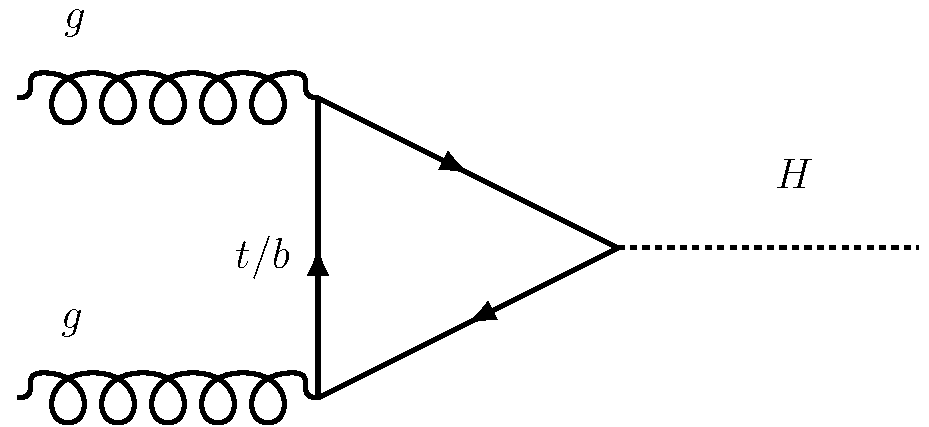
\includegraphics[width=0.5\textwidth]{figuresTHE/ggF.pdf}
  \end{center}
  \caption{
希格斯玻色子产生模型:领头阶胶子融合产生模式。
}
    \label{fig:ggF}
\end{figure}

\begin{figure}
  \begin{center}
    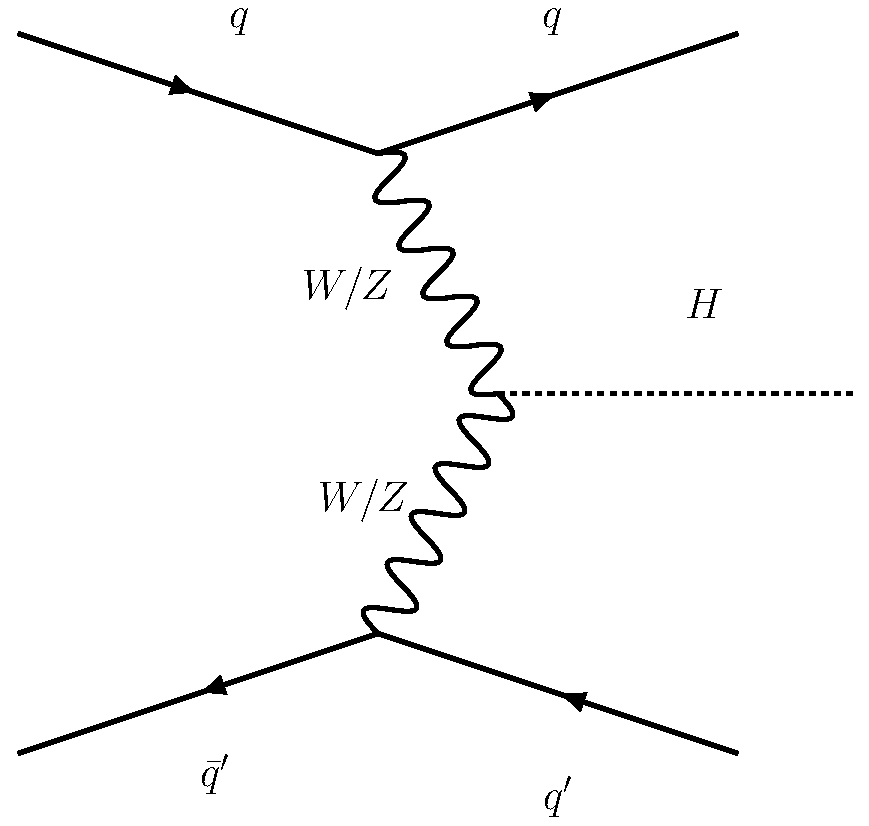
\includegraphics[width=0.5\textwidth]{figuresTHE/VBF.pdf}
  \end{center}
  \caption{
希格斯玻色子产生模式:领头阶矢量玻色子融合。
}
    \label{fig:VBF}
\end{figure}


\begin{figure}
  \begin{center}
    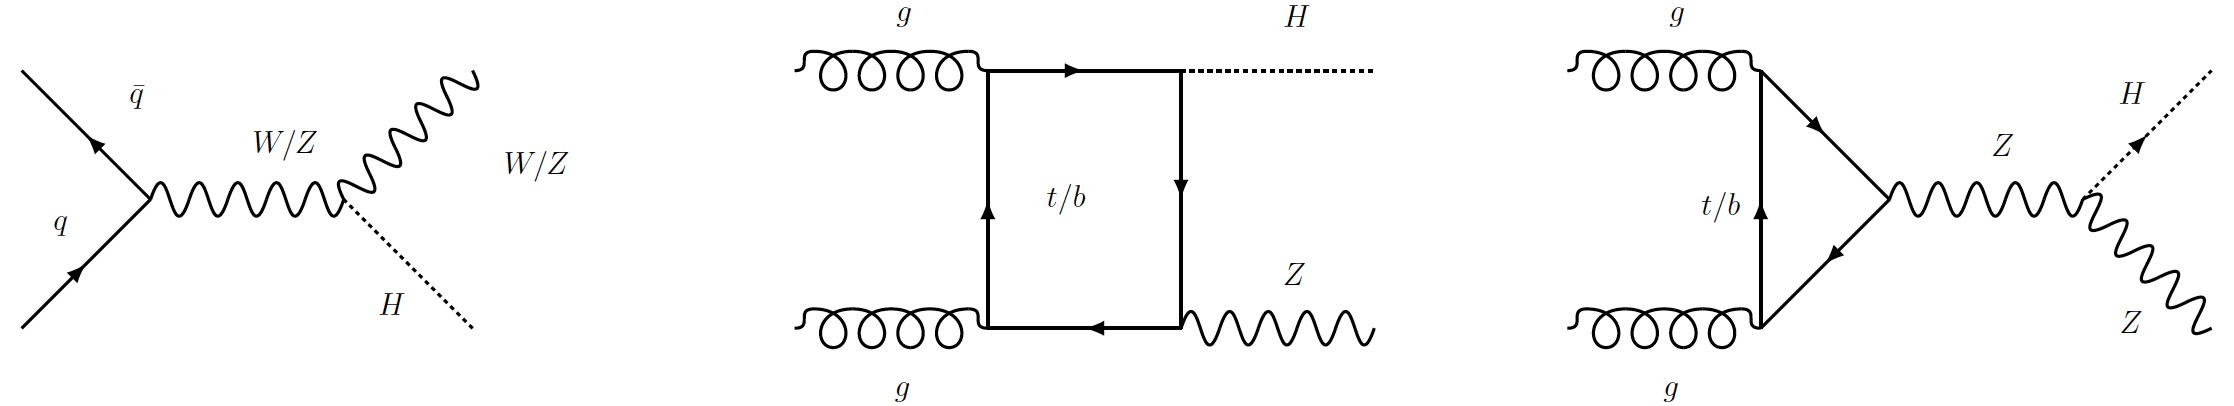
\includegraphics[width=0.98\textwidth]{figuresTHE/WZH.jpg}
  \end{center}
  \caption{
希格斯玻色子产生模型:领头阶矢量玻色子联合产生道。
}
    \label{fig:WZH}
\end{figure}

\begin{figure}
  \begin{center}
    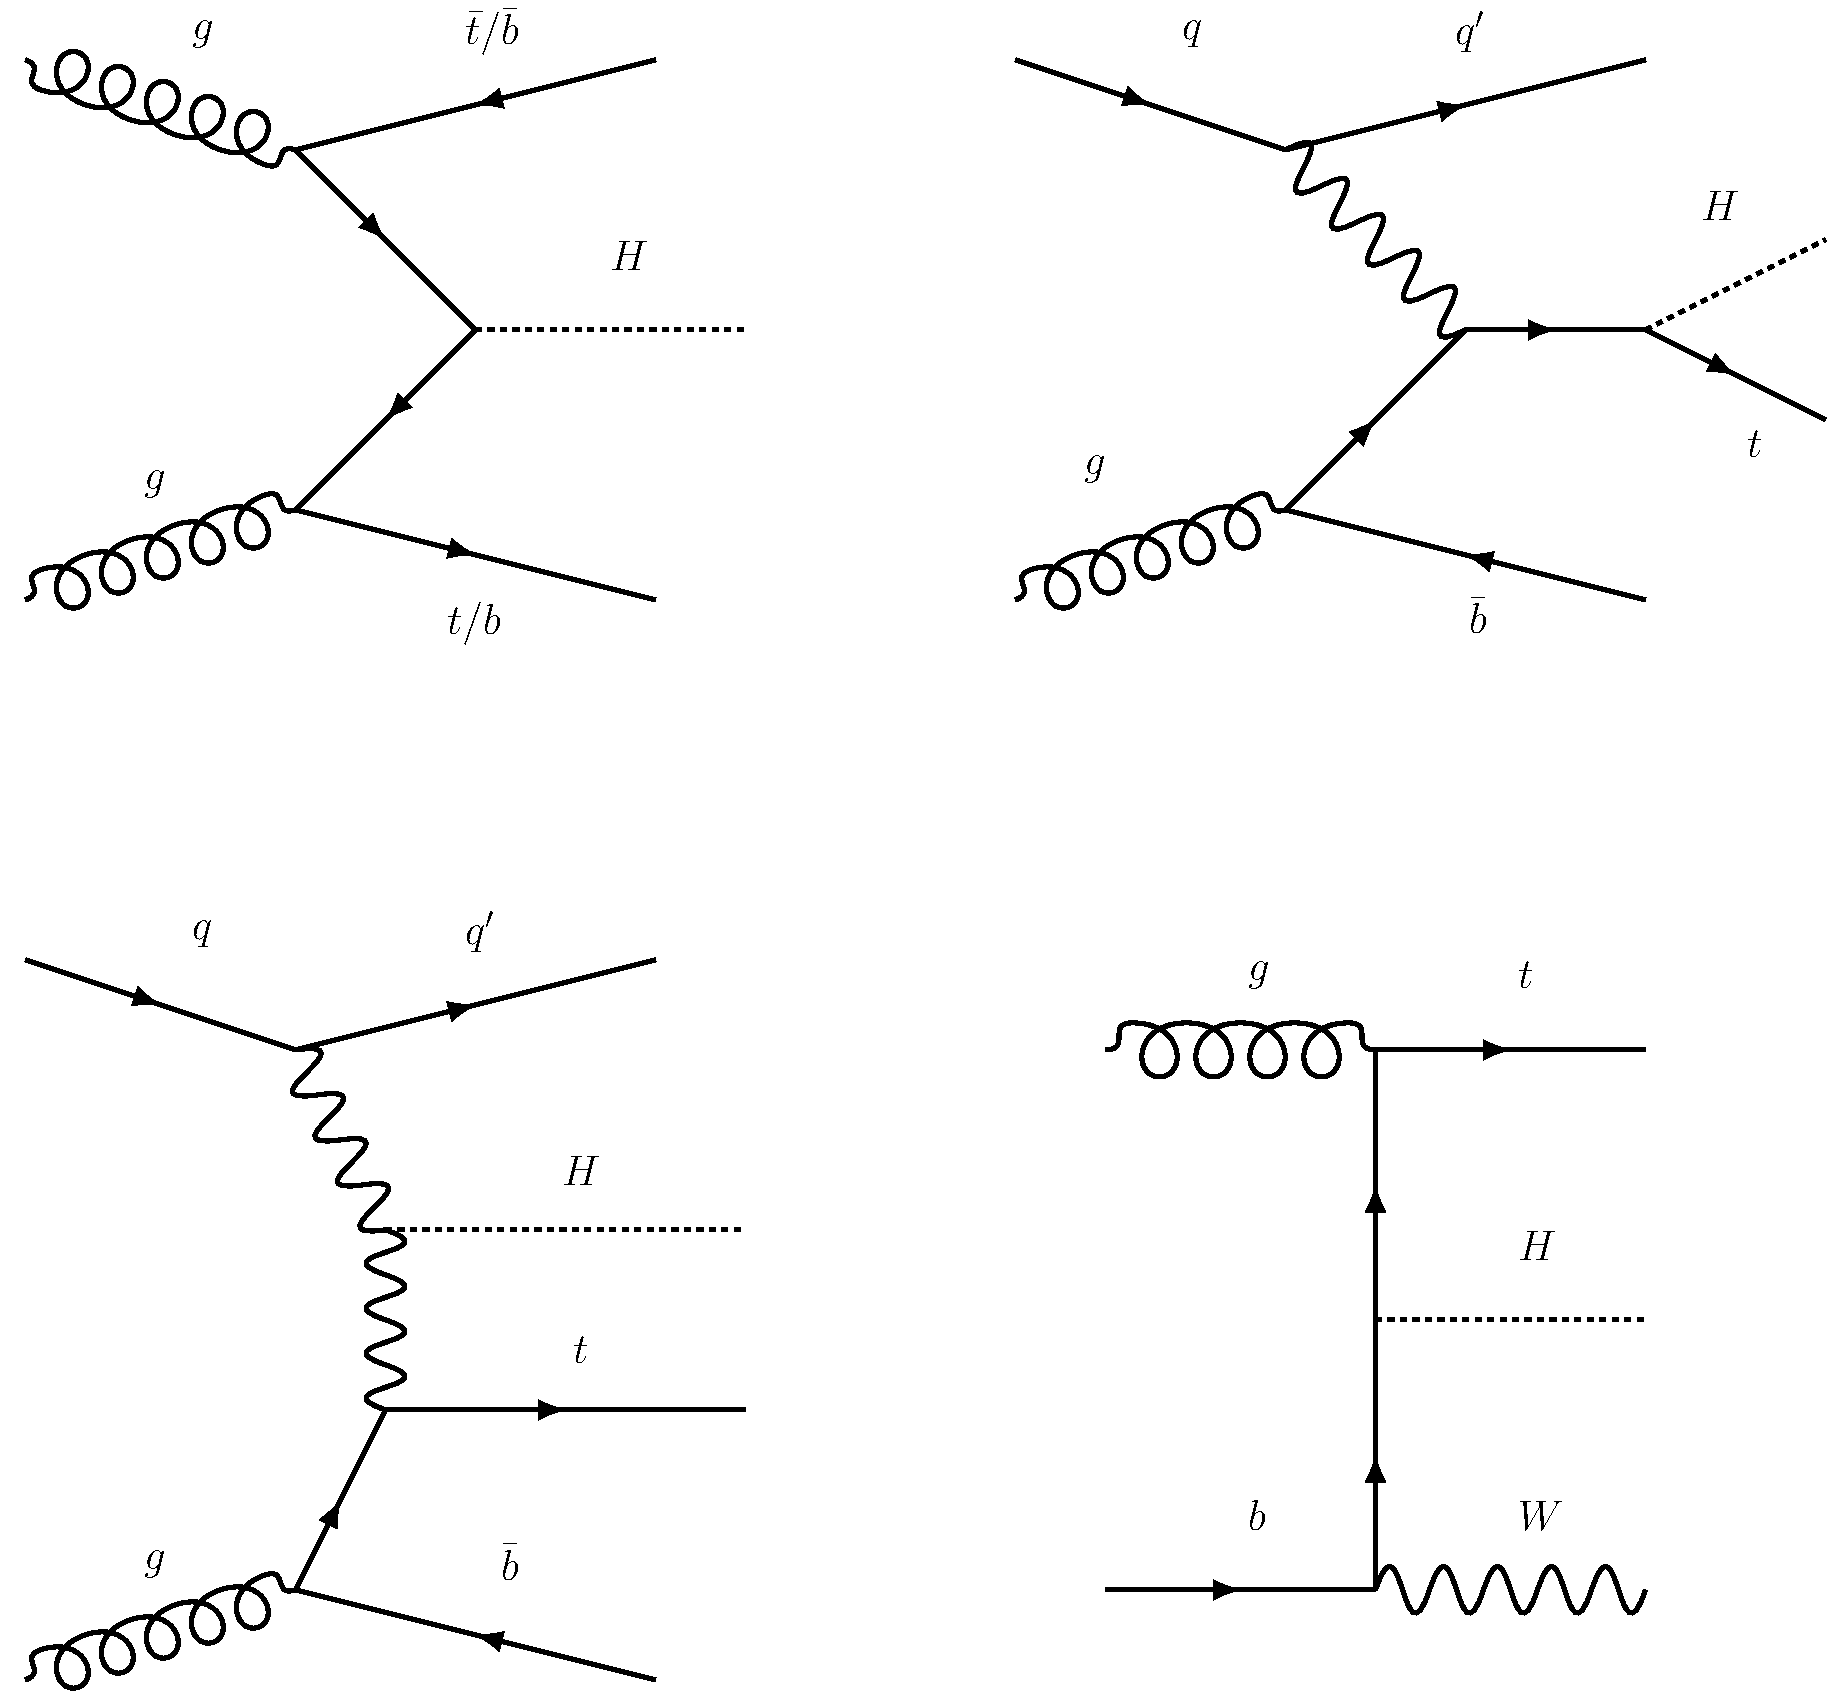
\includegraphics[width=0.85\textwidth]{figuresTHE/ttH.pdf}
  \end{center}
  \caption{
希格斯玻色子产生模式:领头阶矢t夸克联合产生道。
}
    \label{fig:ttH}
\end{figure}

各个产生模式的截面的大小取决于希格斯玻色子质量、碰撞强子的类型和质心系能量。
结合$Run\_1$计划期间ATLAS和CMS所收集的所有数据,测得希格斯玻色子的质量为$m_H=125.09\pm 0.21(stat.)\pm 0.11(syst.)GeV$~\cite{HIGGSMASS}。
图~\ref{fig:SM23}~中左图给出了LHC上质子-质子对撞的质心系能量固定为$\sqrt{s}=13TeV$时,不同产生模式的截面随着希格斯玻色子质量的变化关系,
而右图展示了在希格斯玻色子质量为$M_H=125GeV$情况下,不同产生模式的截面随着质心系能量的变化关系。


\begin{figure}  
  \begin{center}
    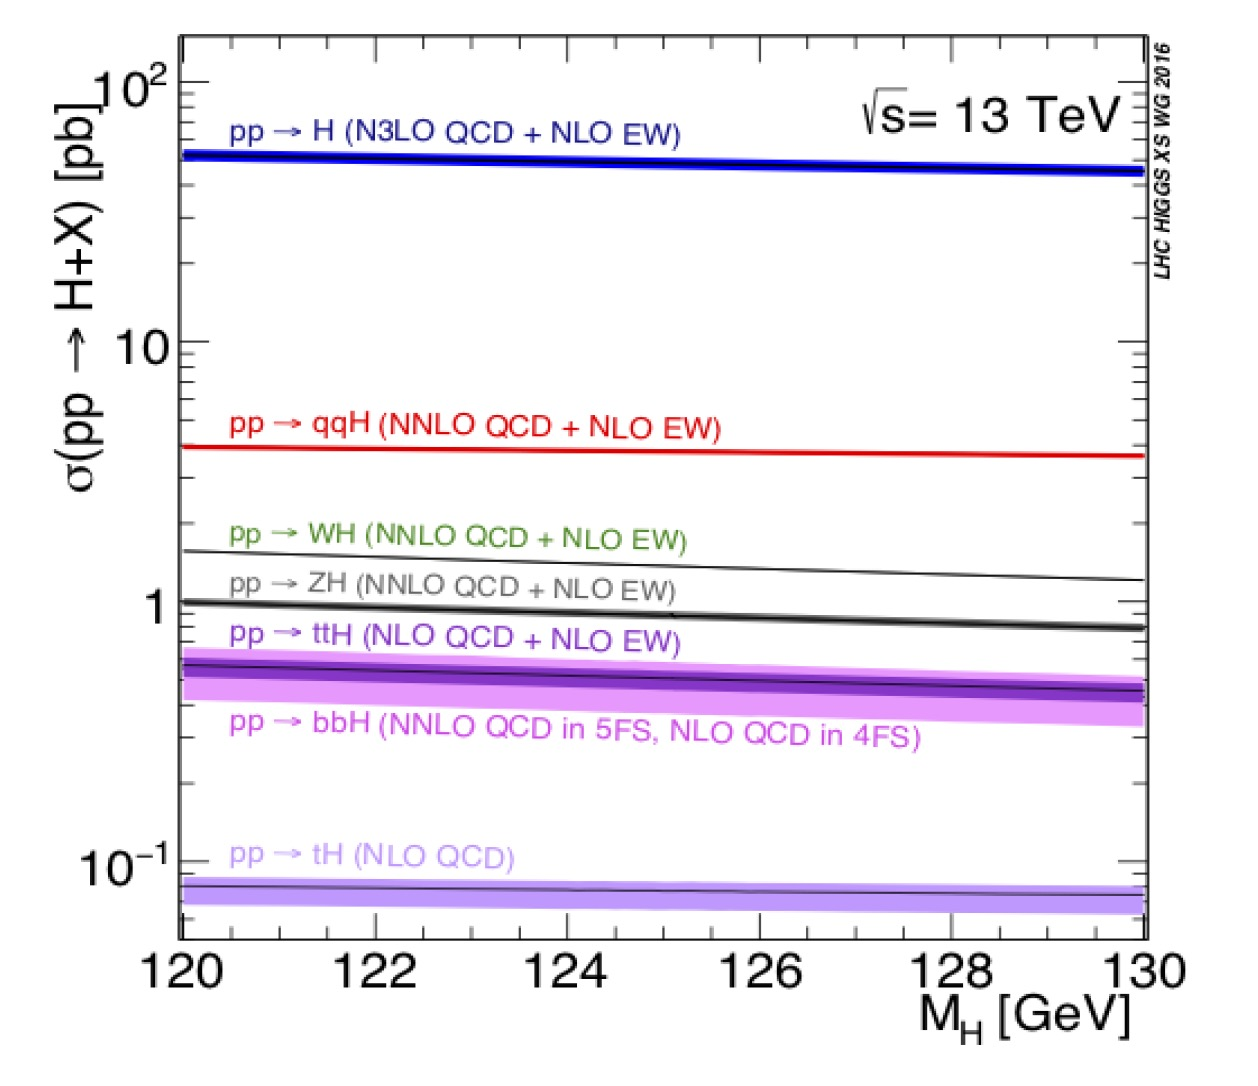
\includegraphics[width=0.49\textwidth]{figuresTHE/SM2.jpg}
    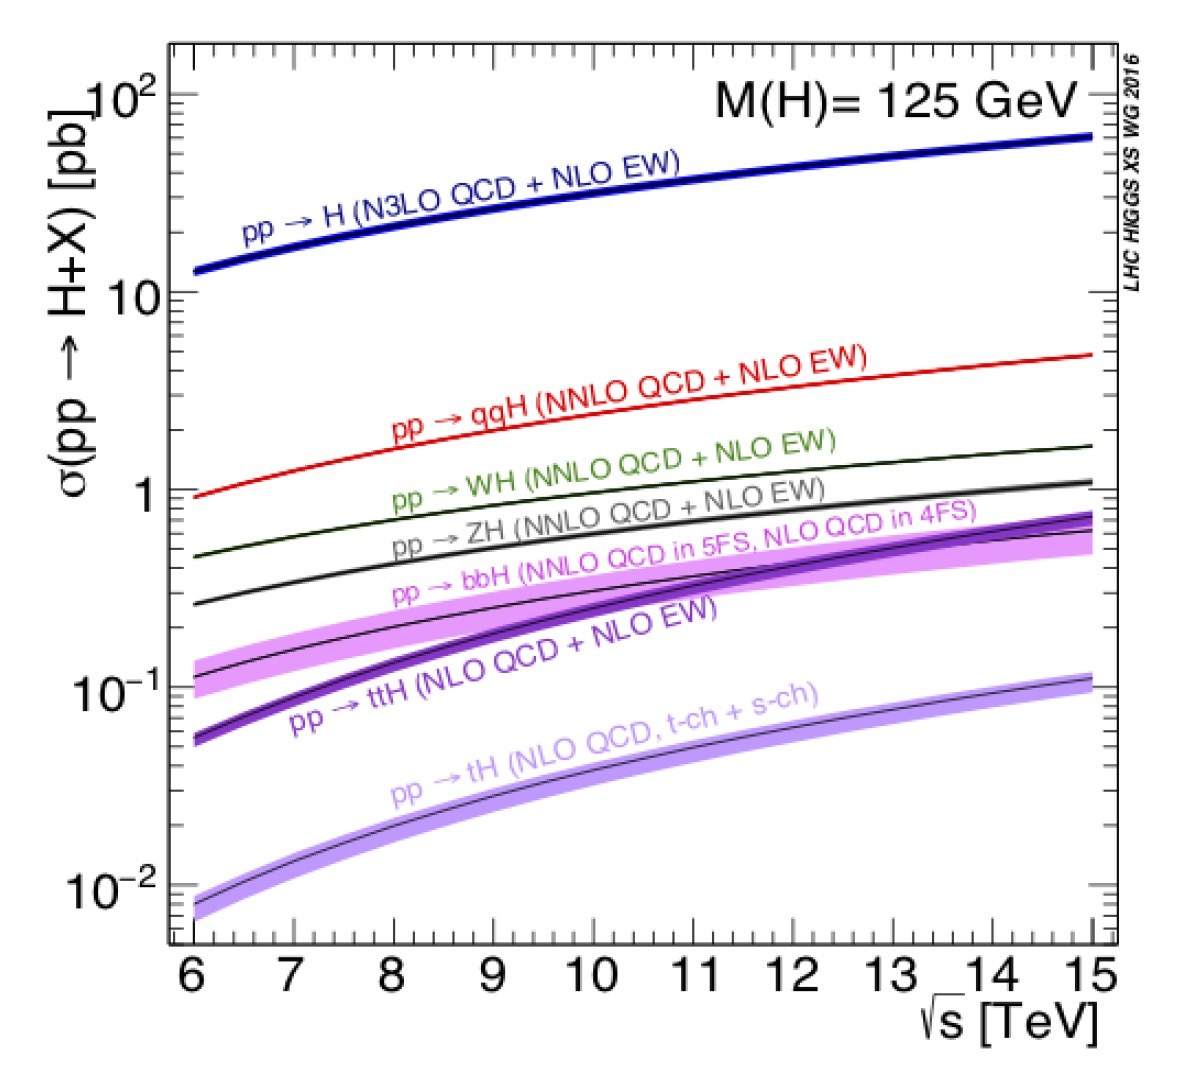
\includegraphics[width=0.49\textwidth]{figuresTHE/SM3.jpg}
  \end{center}
  \caption{
  LHC上质子-质子对撞的质心系能量固定为$\sqrt{s}=13TeV$时,不同产生模式的截面随着希格斯玻色子质量的变化关系(左图),
以及希格斯玻色子质量为$M_H=125GeV$时,不同产生模式的截面随着质心系能量的变化关系(右图)。
    }
  \label{fig:SM23}
\end{figure}



\subsection{希格斯玻色子的衰变}
\label{sec:HiggsDC}

为了表征不同衰变模式的相对强度,引入
衰变分支比(Branching ratio, BR),
它是指相对于衰变粒子的总数,
以单独的衰变模式f进行衰变的粒子所占的分数,
它与部分衰变宽度和总衰变宽度$\Gamma$有关:
\begin{equation} 
\label{eq:HiggsDC1}
BR(H \rightarrow f)= \frac{\Gamma(H \rightarrow f)}{\sum_f \Gamma(H \rightarrow f)}
\end{equation}
如图~\ref{fig:SM45}~所示,是标准模型预言的希格斯玻色子不同模式的衰变分支比与希格斯玻色子质量的关系~\cite{HANDHIGGS},
左图所示质量区间为80到120GeV,右图是120到130GeV。

\begin{figure}  
  \begin{center}
    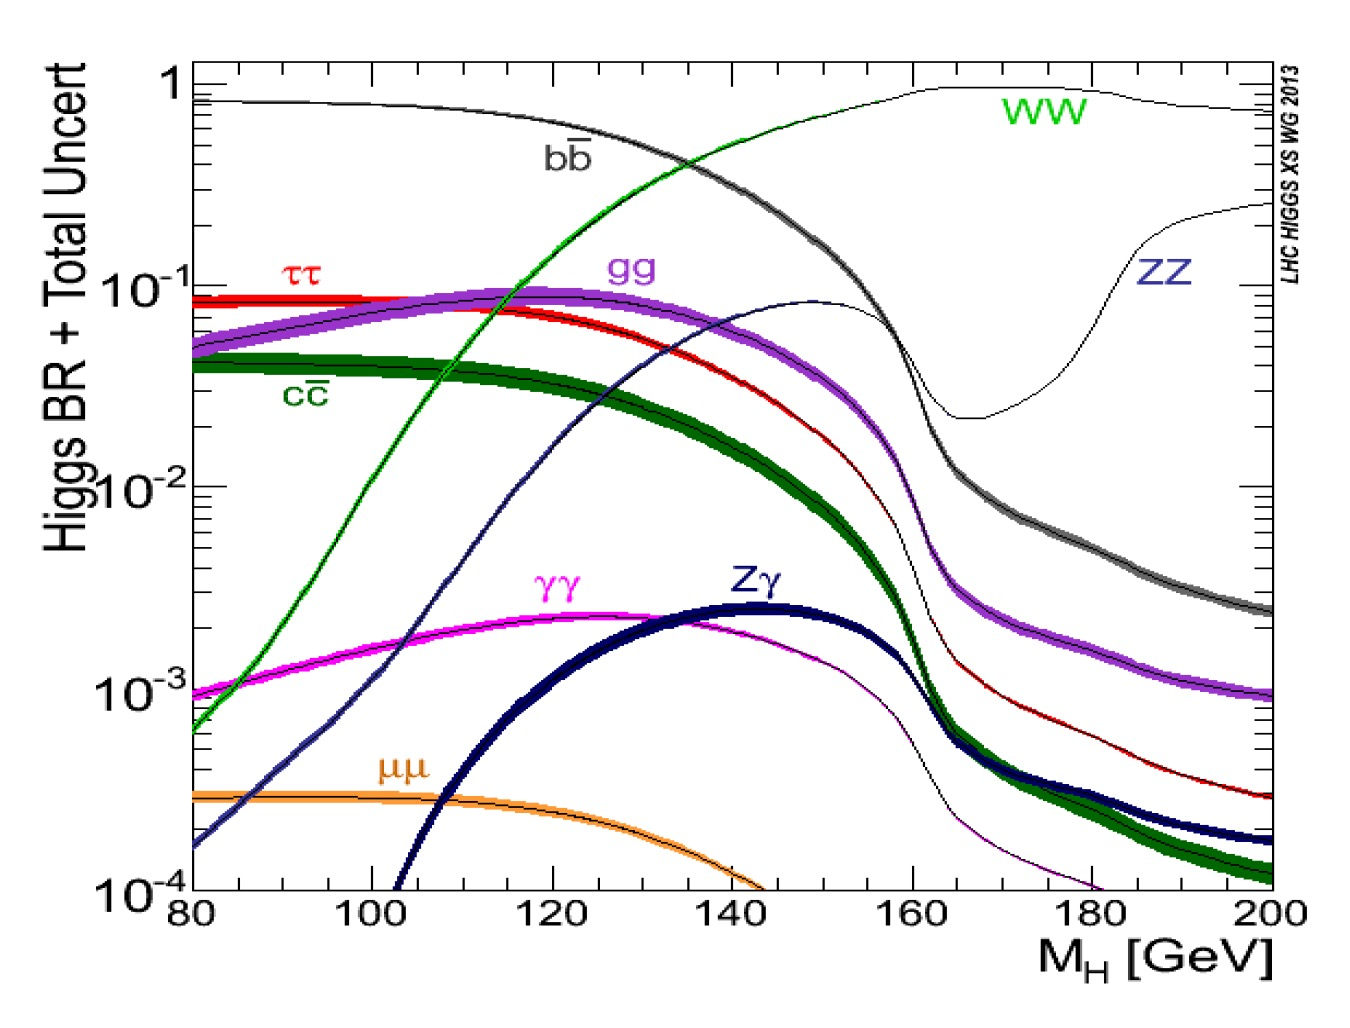
\includegraphics[width=0.49\textwidth]{figuresTHE/SM4.jpg}
    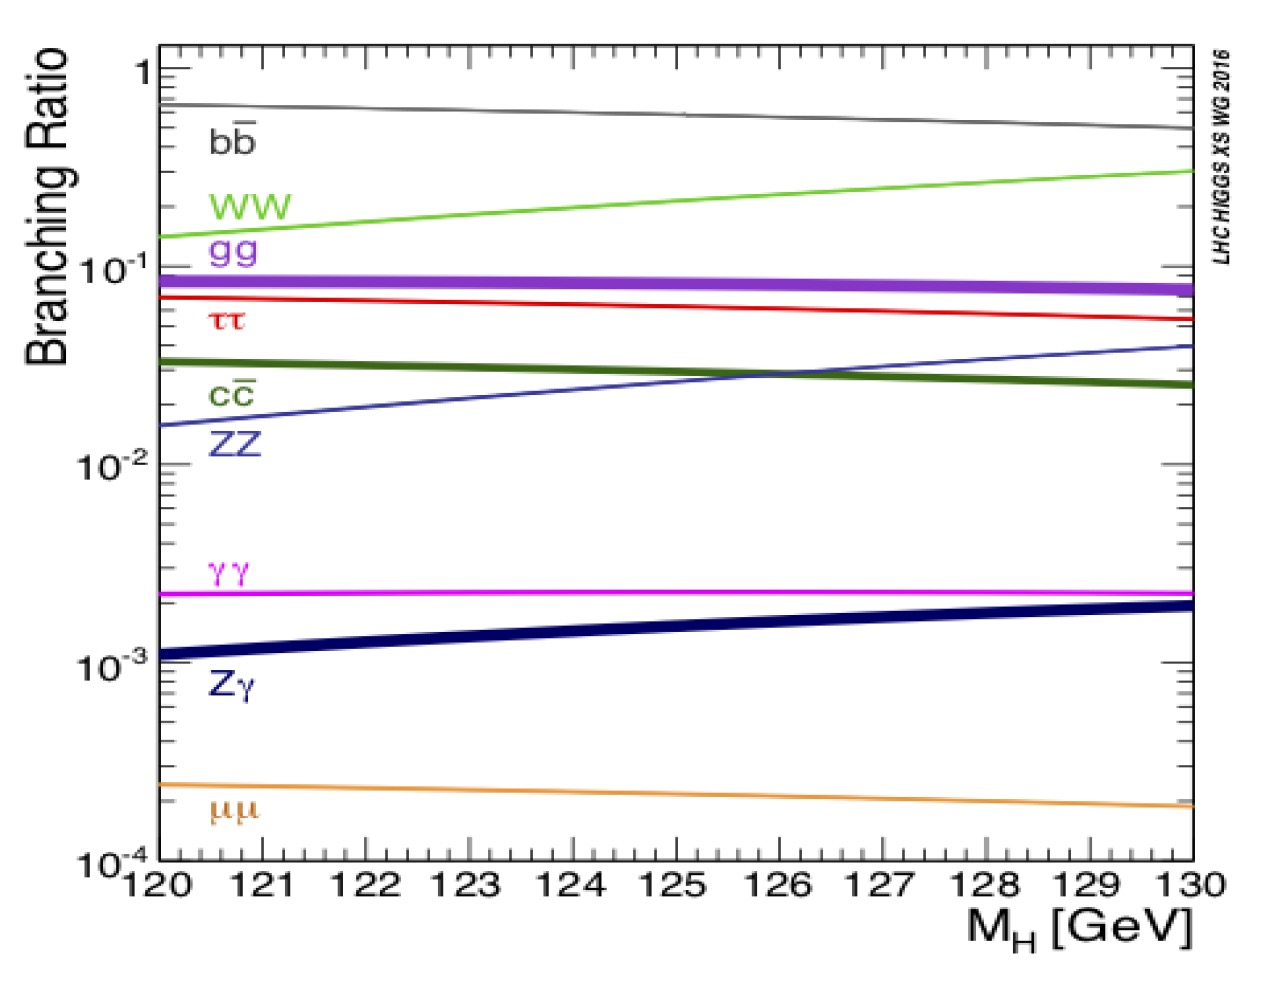
\includegraphics[width=0.49\textwidth]{figuresTHE/SM5.jpg}
  \end{center}
  \caption{
希格斯玻色子不同模式的衰变分支比与希格斯玻色子质量的关系。左图所示质量区间为80到120GeV,右图是120到130GeV。
    }
  \label{fig:SM45}
\end{figure}

表~\ref{tab:SMTab1}~列出了当希格斯玻色子质量取$M_H=125GeV$时,各个可能衰变模式的衰变分支比。
如前面所指出的,由于费米子与希格斯玻色子的耦合强度与费米子质量成正比,
因此在末态为费米子的衰变模式中,希格斯玻色子更加倾向于衰变成质量较大的费米子。

\begin{table}[htbp]
      \caption{在希格斯玻色子质量为$m_H=125GeV$时,标准模型中希格斯玻色子各个衰变模式的衰变分支比。}
      \label{tab:SMTab1}
      \centering
      
%      \begin{tabular}{|c|c|c|c|c|c|c|c|c|}
 %       \hline
 %        Decay channel~$(H \rightarrow )$ & $b \bar{b}$ & $W^+W^-$ & $gg$ & $\tau^+\tau^-$ & $ZZ$ & $\gamma\gamma$ & $Z\gamma $& $\mu^+\mu^-$ \\
 %       \hline
 %        Branching ratio & $5.81\times 10^{-1}$ & $2.15\times 10^{-1}$ & $8.18\times 10^{-2}$ & $6.26\times 10^{-2}$ & $2.64\times 10^{-2}$ & $2.27\times 10^{-3}$ & $1.54\times 10^{-3}$ & $2.17\times 10^{-4}$   \\
 %       \hline
 %    \end{tabular}
      \begin{tabular}{|c|c|}
      \hline
      Decay channel~$(H \rightarrow )$ & Branching ratio \\
       \hline
        $b \bar{b}$ & $5.81\times 10^{-1}$   \\
         \hline
        $W^+W^-$ &  $2.15\times 10^{-1}$ \\
         \hline
        $gg$  &  $8.18\times 10^{-2}$  \\
         \hline
        $\tau^+\tau^-$  &  $6.26\times 10^{-2}$  \\
         \hline
        $ZZ$  & $2.64\times 10^{-2}$  \\
         \hline
        $\gamma\gamma$  & $2.27\times 10^{-3}$   \\
         \hline
        $Z\gamma $ & $1.54\times 10^{-3}$  \\
         \hline
        $\mu^+\mu^-$ & $2.17\times 10^{-4}$  \\
        \hline 
      \end{tabular}
\end{table}


\subsection{高横动量希格斯玻色子衰变到双b夸克的标定动机}
\label{sec:BoostedHiggs}

%而对于所测定的质量,标准模型预测的衰变分支比最大的模式是$H\rightarrow b \bar{b}$,达到了$58\%$,
%但也由于QCD和t夸克本底比较大,使得该衰变模式的鉴定非常困难。
%在这个背景下,第~\ref{cha:Xbb}~章介绍了一种基于机器学习的标定算法,
%用于标定高横动量的$H\rightarrow b \bar{b}$,
%它不仅实现了质量去关联,而且还能保持非常出色的本底排除率。
%其中,尽管$H\rightarrow b\bar{b}$衰变道是希格斯玻色子的主要衰变模式,占高达$58\%$的分支比,

对于实验测定的希格斯质量,
从表~\ref{tab:SMTab1}~中可以看到$H\rightarrow b\bar{b}$衰变道是希格斯玻色子的主要衰变模式,
所占分支比高达$58\%$,
但也由于来自QCD过程和t夸克衰变的本底非常大,使得在LHC上面观测这个衰变模式变得很困难。
通过要求事例中包含孤立的轻子,可以显著的降低QCD本底,因此寻找$H\rightarrow b\bar{b}$衰变道灵敏度最高的产生模式是VH,
在2018年,ATLAS合作组和CMS合作组分别利用$79.8fb^{-1}$和$41.3fb^{-1}$的数据通过VH产生模式观测到显著的$H\rightarrow b\bar{b}$事例,
显著性分别达到了4.9和4.8倍的标准差~\cite{AHbb8,CHbb3},
随后在2020年,ATLAS合作组利用$139fb^{-1}$的数据观测到了更加丰富的$H\rightarrow b\bar{b}$事例~\cite{AHbb5}。
但是也有一部分研究通过其他产生模式来测定$H\rightarrow b\bar{b}$衰变道,
比如$t\bar{t}H$~\cite{AHbb7,AHbb8,CHbb1}、VBF~\cite{AHbb6}和高横动量区的ggF~\cite{CHbb3}。

而高横动量的$H\rightarrow b\bar{b}$衰变与低横动量的$H\rightarrow b\bar{b}$衰变的拓扑性质不一样,
如图~\ref{fig:Boosted1}~所示,在探测器中,来自高横动量希格斯玻色子衰变的两个b夸克接近准直,
会合并到一个大的喷注即LR-jet当中,将会在第~\ref{sec:JET}~小节介绍LR-jet的概念,
通过其整体性可以更加容易的鉴定$H\rightarrow b\bar{b}$事例。
%依靠其整体性使得$H\rightarrow b\bar{b}$事例更容易鉴定。
而且在许多超出标准模型的新物理模型中~\cite{BSMHIGGS1,BSMHIGGS2,BSMHIGGS3}都引入了能与标准模型中希格斯玻色子耦合的新粒子的存在,
这些新粒子的质量都很大,衰变产生的希格斯玻色子将会具有很高的横动量。
因此对高横动量的$H\rightarrow b\bar{b}$衰变的
%研究或者
标定对希格斯玻色子性质的精确测量和新物理的寻找都有着重要意义。
这篇论文第~\ref{cha:Xbb}~章中便介绍了一种基于机器学习的标定算法,用于标定高横动量$H\rightarrow b \bar{b}$衰变。


\begin{figure}
  \begin{center}
    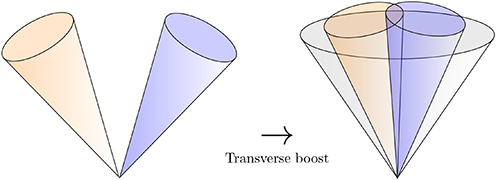
\includegraphics[width=0.75\textwidth]{figuresXbb/Boosted.jpg}
  \end{center}
  \caption{
来自高横动量希格斯玻色子衰变的两个b夸克接近准直,从而合并到一个LR-jet当中。
  }
    \label{fig:Boosted1}
\end{figure}







\section{超出标准模型的新物理}
\label{sec:BSM}

在标准模型建立的过程中,
实验上不断的以极高的精度验证了其正确性,
%其不断的以极高的准确性得到了验证,
并且在理论预测和实验观测之间也保持着高度的一致。
但是,仍然存在一部分标准模型不能解释的现象。

标准模型未能解释暗物质~\cite{DARKMATTER1}从何而来,也没有提供暗物质的候选粒子。
在1930年,F. Zwicky观测到后发星系团(Coma cluster)中星系的速度弥散(Velocity dispersion)约为1000$km~s^{-1}$,
这比根据实际发光物质所估计的速度弥散80$km~s^{-1}$要大的多,
这表明存在“看不见”的物质即暗物质为星系团提供额外的吸引力将星系保持在星系团内部~\cite{DARKMATTER2}。
在那以后,有更多的实验证据为暗物质提供了有力的支持~\cite{DARKMATTER1},
根据宇宙学观测的结果,暗物质贡献了宇宙总物质的$27\%$,
而标准模型所描述的基本粒子仅占$5\%$。

标准模型中未包含引力。引力作为一种基本的相互作用,可以由广义相对论~\cite{GRE}来描述,
标准模型虽然统一了强、弱和电磁相互作用,但是它不能在量子场论的框架下诠释引力的规范理论。
其中重要的原因是,标准模型中引入引力子之后将不具有可重整性~\cite{GRE1},
而且电弱相互作用和引力相互作用之间存在层级问题(The hierarchy problem)~\cite{HP},
电弱对称破缺的能标($\sim 10^{2}GeV$)比引力的基础能标即普朗克能标($\sim 10^{19}GeV$)小多个数量级。

还有诸如Yukawa耦合常数的层级问题、中微子质量起源和宇宙中正反物质不对称等问题。
都表明了标准模型本身并不是完整的,不能作为物质世界的终极理论。



\subsection{在双喷注末态的不变质量谱中寻找新物理的动机}
\label{sec:BSMDijet}

为了解决这些问题,理论物理学家发展了许多超出标准模型的新物理理论(Physics beyond the Standard Model, BSM)。
其中的一部分新物理模型~\cite{qstar1,qstar2,zprime1,zprime3,wprime1,Chizhov:2009fc,Chizhov:2010jg,DM1,DM2,DM3,qbh1,qbh2,RS1,RS2,ADD}
预言了能与标准模型中夸克($q$)或者胶子($g$)耦合的新的重粒子的存在,
这些新粒子如果存在的话能通过高能质子-质子对撞产生,并衰变成两个能量很高的夸克或者胶子,
以两个喷注即jet的形式被探测器探测到,将会在第~\ref{sec:JET}~小节介绍jet的概念,
图~\ref{fig:BSMDijet1}~为该过程所对应的费曼图~\cite{FEYNR}。
在标准模型中,双喷注末态事例主要来自于QCD过程,
而QCD预言的双喷注末态的不变质量谱$m_{jj}
$\footnote{自然单位制下,两个物理对象的不变质量定义为$m_{12}=\sqrt{(E_1+E_2)^2-(\vec{p_1}+\vec{p_2})^2}$,其中($E_1$,$\vec{p_1}$)、($E_2$,$\vec{p_2}$)分别为两个物理对象的能量和动量。}
是平滑下降的,
若是有一个非标准模型的新粒子衰变到两个夸克或者胶子,在QCD预言的平滑下降的$m_{jj}$上便会出现一个共振峰,
对应于新粒子的质量,可以通过这个手段来寻找新物理~\cite{UA3}。
这篇论文第~\ref{cha:Dijet}~章介绍的物理分析便是通过在双喷注末态的不变质量谱上搜索局部突出的共振峰,在TeV量级的高质量区间寻找超出标准模型的新粒子。
这里选取了其中一部分新物理模型作为基准模型来优化分析,同时用来评估同类型分析的进展。

\begin{figure}
  \begin{center}
    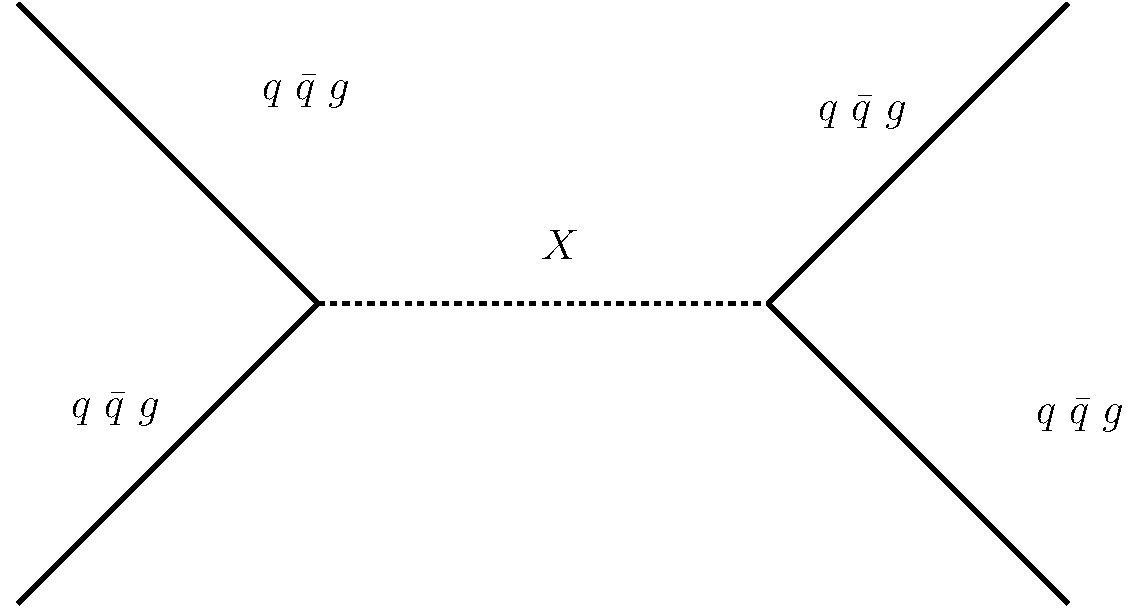
\includegraphics[width=0.5\textwidth]{figuresTHE/SChl.pdf}
  \end{center}
  \caption{
新粒子的产生模式。其中X表示新粒子。
}
    \label{fig:BSMDijet1}
\end{figure}


%为了解决这些问题,理论物理学家发展了许多超出标准模型的新物理理论(Physics beyond the Standard Model, BSM)。
%如图~\ref{fig:SChl}~所示,第~\ref{cha:Dijet}~章中的分析旨在通过新物理共振态的s道产生模式来寻找超出标准模型的新物理~\cite{FEYNR},
%并选取了一些新物理模型作为基准模型来优化分析,同时用来评估同类型分析的进展。
%这里将简要介绍这些所选的基准理论模型和它们背后的动机。


%\begin{figure}
 % \begin{center}
   % 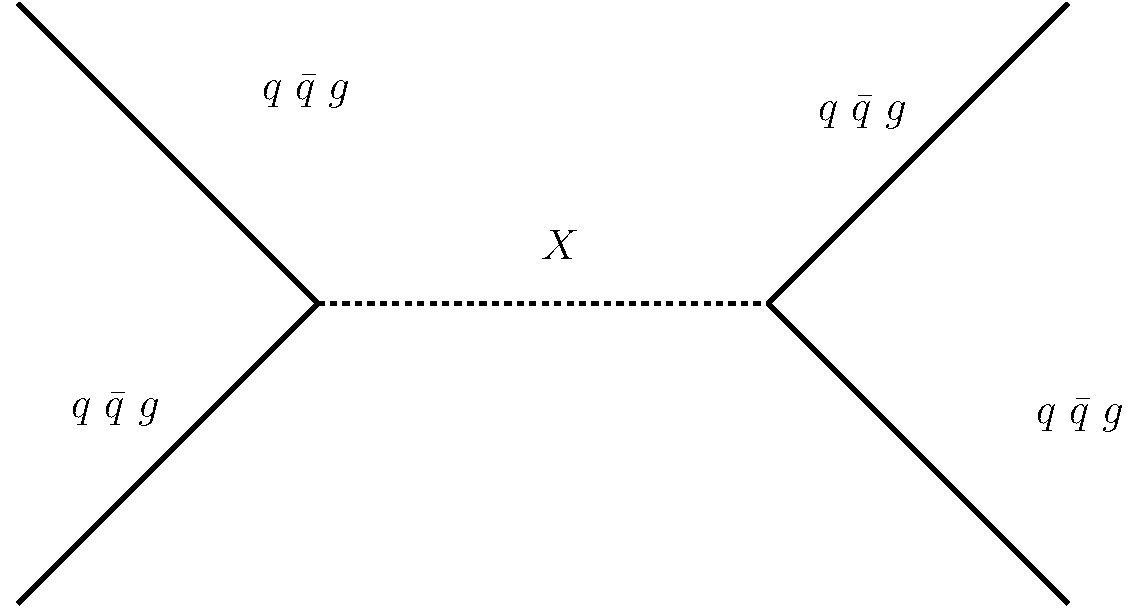
\includegraphics[width=0.5\textwidth]{figuresTHE/SChl.pdf}
  %\end{center}
  %\caption{
%新物理共振态的s道产生模式。
%}
  %  \label{fig:SChl}
%\end{figure}


\subsection{暗物质$Z'$模型}
\label{sec:ZPrime}

暗物质$Z'$模型~\cite{DM1,DM2,DM3}是将标准模型中的基本粒子与暗物质媒介子$Z'$和暗物质候选粒子$\chi$联系起来的一个模型,
其中暗物质媒介子$Z'$是一个来自额外$U(1)$规范群的轴矢量玻色子,
如图~\ref{fig:ZChl}~所示,它能与暗物质费米子$\chi$耦合,也可以与标准模型中夸克耦合,
对应的拉氏量为:
\begin{equation} 
\label{eq:ZPrime1}
\mathcal{L}_{axial-vector}=g_{\chi} Z'_{\mu} \bar{\chi} \gamma^{\mu} \gamma^5 \chi +
g_{SM} \sum_{q=u,d,s,c,b,t} \left( Z'_{\mu} \bar{q} \gamma^{\mu} \gamma^5 q \right)
\end{equation}
其中$g_{SM}$是
%暗物质媒介子
$Z'$与标准模型中夸克的耦合常数,
$g_{\chi}$是$Z'$与
%暗物质费米子
$\chi$之间的耦合常数,
$Z'$和$g_{\chi}$的质量也是模型中的未知参数。
通过$Z'$与夸克之间的耦合可以在探测器上寻找$Z'$。

\begin{figure}
  \begin{center}
    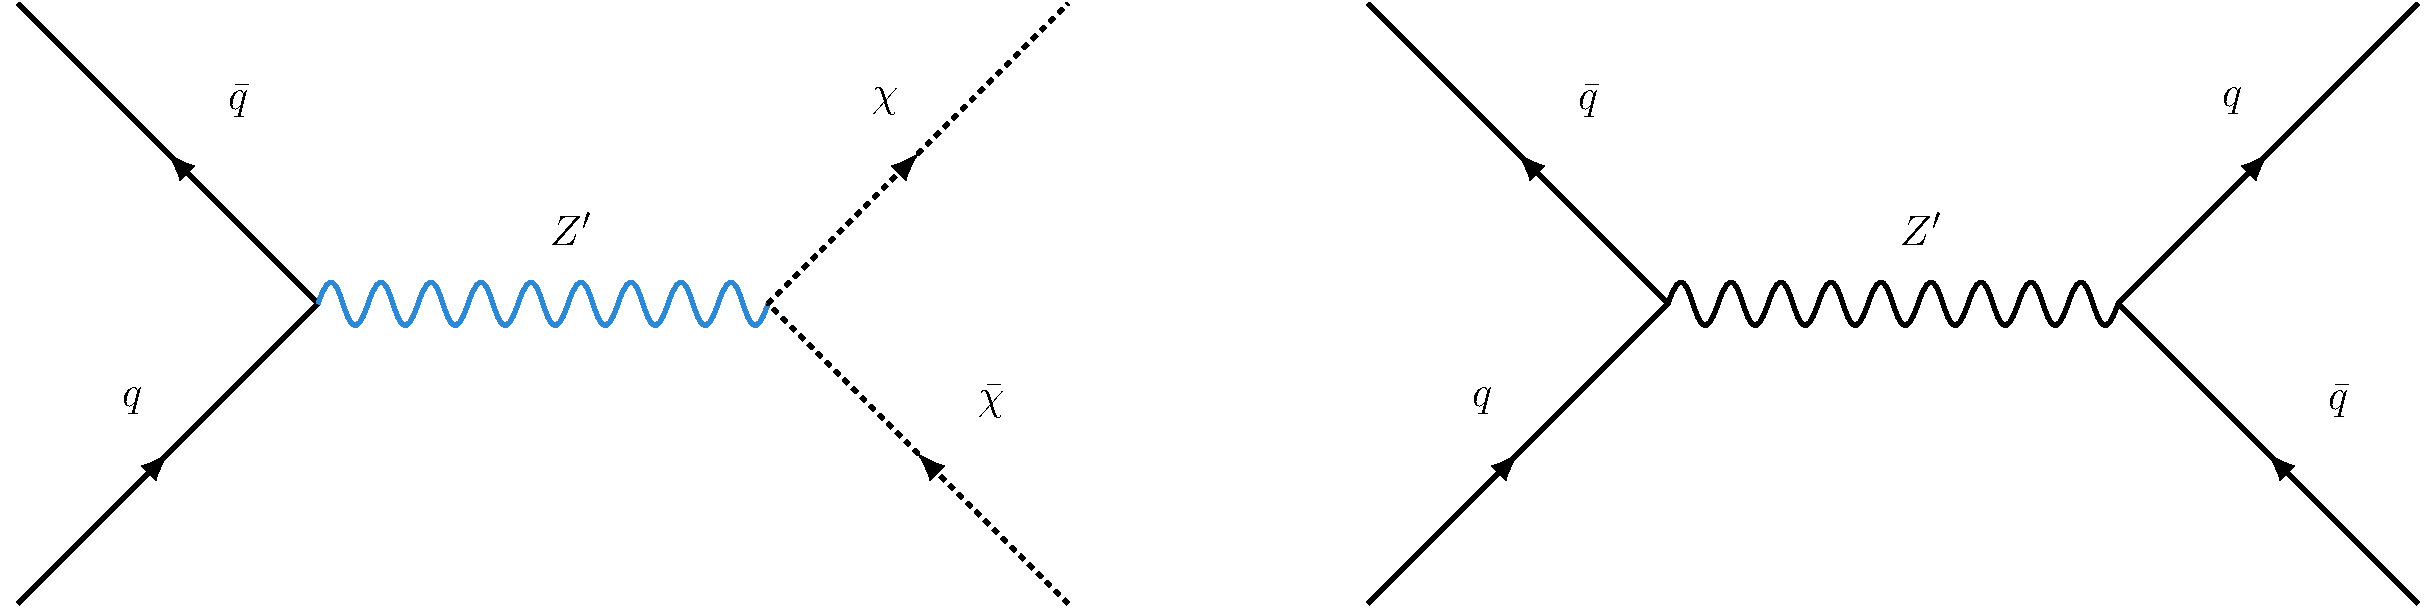
\includegraphics[width=0.9\textwidth]{figuresTHE/ZChl.pdf}
  \end{center}
  \caption{
暗物质媒介子$Z'$的两种衰变模式。左图$Z'\rightarrow \chi+\bar{\chi}$。右图$Z'\rightarrow q+\bar{q}$。
}
    \label{fig:ZChl}
\end{figure}

\subsection{Kaluza-Klein引力子和量子黑洞}
\label{sec:KKG}
作用力之间的层级问题使得引力比其他相互作用弱很多。
可能的一个解释是,引力本来与其他相互作用有着比较接近的强度,
但是因为它可以在更高维的时空中传播,在可观测的四维时空中就表现很弱。
基于这种猜想,有两种主流的额外维理论模型:Randall-Sundrum模型~\cite{RS1,RS2}和
Arkani-Hamed Dimopoulos Dvali模型~\cite{ADD}。
模型中高维时空的引入可以将引力的基础能标降低到TeV的量级,
相应的Kaluza-Klein(KK)引力子便可以在LHC上产生并衰变成两个夸克或者胶子,
同时质量在TeV量级的量子黑洞~\cite{qbh1,qbh2}也可以在LHC上形成并衰变成两个夸克或者胶子,
在一定的质量范围内被探测器探测到。

%\subsection{量子黑洞}
%\label{sec:QBH}
%上述高维时空引入之后,在降低引力能标的同时,
%LHC上高能质子-质子对撞也可能形成质量在TeV量级量子黑洞~\cite{qbh1,qbh2},
%并且能衰变到夸克或者胶子。


\subsection{重规范玻色子}
\label{sec:WZPrime}
在许多BSM理论中,都引入了额外的规范对称性,
从而会出现新的规范玻色子。
这里考虑了连续标准模型(The Sequential Standard Model, SSM)~\cite{zprime1,zprime3,wprime1}中
质量比较大的两种规范玻色子$W'$和$Z'$,
它们的质量也在TeV尺度,能衰变到两个夸克。

\subsection{激发态夸克}
\label{sec:QStar}
激发态夸克$q^*$~\cite{qstar1,qstar2}来自于一种复合夸克模型,模型中$q^*$的不是基本粒子,
而是具有内部结构的束缚态,能衰变到一个夸克和一个胶子。
模型的出发点是为了解释夸克质量的层级结构和三代问题。

\subsection{手征激发态玻色子$W^*$}
\label{sec:WStar}

手征激发态玻色子$W^*$~\cite{Chizhov:2009fc,Chizhov:2010jg}来自于一个拓展模型,
其将标准模型中弱相互作用的规范群$SU(2)$扩展成$SU(3)$,
相应的对称性自发破缺的能标在TeV量级。
%并通过TeV能标的对称性自发破缺。
%模型中会出现一个相应的带电矢量玻色子$W^*$,它能与标准模型中的费米子耦合。






















% !TeX root = ../main.tex


\chapter{实验}
\label{cha:EXP}

标准模型和超出标准模型的新物理理论所预测的基本粒子和基本相互作用的强度能在自然界中得以体现。
因此,需要通过实验对比数据中的观测量和理论的预测值,用以验证理论的有效性。
而由欧洲核子研究中心(CERN)建造的大型强子对撞机(LHC)就是用于检验这些理论有效性的装置。

本章第~\ref{sec:LHC}~小节将简要介绍LHC和它的运行计划。
第~\ref{sec:ATLAS}~小节则会简要介绍LHC上ATLAS探测器及其各个组成部分,
因为这篇论文的研究工作都是基于ATLAS实验。
第~\ref{sec:Simulation}~小节会简要介绍一下模拟的实现技术,
第~\ref{sec:Reconstruction}~小节将介绍ATLAS探测器中物理对象的重建技术,尤其是喷注的重建过程。

\section{大型强子对撞机}
\label{sec:LHC}

LHC~\cite{Evans:2008zzb}是至今为止人类建造的规模最大的、功能最强的粒子加速器。
由于体型庞大,它被建于CERN地下约100米的混凝土内衬隧道当中。
LHC是一个圆形的粒子对撞机,总周长约为26.7千米,穿过欧洲日内瓦中心、法国侏罗山脉以及法国和瑞士的边界等地区。
根据实验设计,LHC可以将两个束流中的质子加速到高达7TeV的能量,随后两束反向的质子束流会在四个相互作用点相交并发生碰撞。
其中大约有1232个由Nb和Ti组成的偶极超导磁铁,处于1.9K的工作温度下,
为质子束流提供高达8.3T的磁场,并使它们沿特定的圆形轨道运动。
另外有大约392个四极磁铁负责束流的聚焦,16个射频腔为束流加速。
%其中有1232个处于1.9K温度下由Nb和Ti组成的偶极超导磁铁保证质子束流在高达8.3T的磁场中沿特定的圆形轨道运动,392个四级磁铁负责束流的聚焦,16个射频腔为束流加速。

在进入LHC大环之前,质子束流会经历多个加速阶段,如图~\ref{fig:LHC1}~所示是CERN整个加速器系统的结构~\cite{LHCImage1}。
首先,将氢原子中的电子剥离之后,剩下的质子会被注入到直线加速器\textsc{Linac2}当中,在这里质子的能量可以达到50MeV。
然后将它们注入到环形加速器\textsc{Booster}当中,加速至1.4GeV的能量。
随后,会将它们送入环形加速器\textsc{Ps}当中,此时质子束流能量可以达到25GeV。
接着,经过环形加速器\textsc{Sps}加速之后,束流能量达到450GeV。最后进入LHC大环。

\begin{figure}
  \begin{center}
    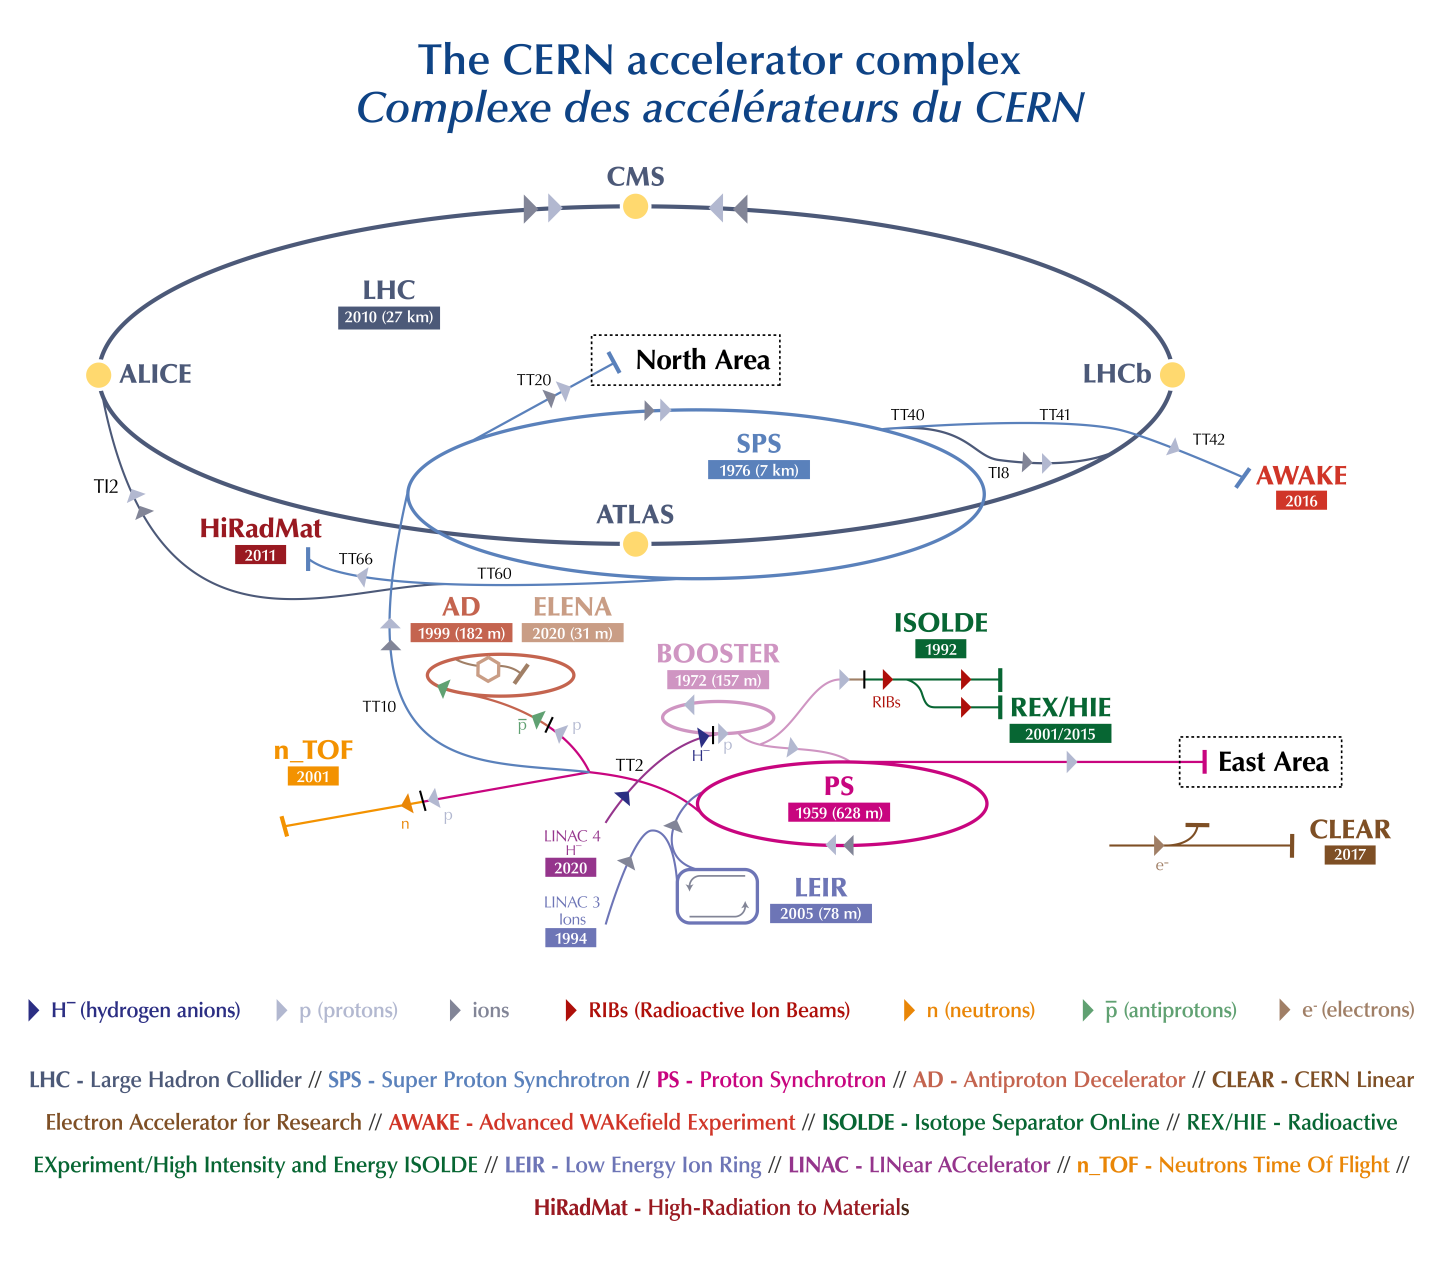
\includegraphics[width=0.75\textwidth]{figuresEXP/LHC1.png}
  \end{center}
  \caption{
CERN加速器系统的结构。首先质子会被注入到直线加速器\textsc{Linac2}当中,
然后将它们注入到环形加速器\textsc{Booster}当中,随后,会将它们送入环形加速器\textsc{Ps}当中,
接着,在经过环形加速器\textsc{Sps}加速之后,最后进入LHC大环,此时质子能量可以达到7TeV。
  }
    \label{fig:LHC1}
\end{figure}


在质子束流由环形加速器\textsc{Sps}向LHC大环转移的过程中,束流会被分成两个单独的束流,分别沿着相反的方向注入到LHC大环当中,然后进行碰撞。
束流中的质子束是以非连续的形式组合在一起的,每个质子束大约含有$10^{11}$个质子。
而单个束流最多包含2808个质子束,质子束与质子束之间碰撞的时间间隔为25ns,碰撞频率高达40MHz。
根据设计,束流能达到最高7TeV的能量,对应的质心系能量为$\sqrt{s}$=14TeV。
瞬时亮度(Instantaneous luminosity)能达到$\mathcal{L}=10^34 cm^{-2}s^{-1}$~\cite{Evans:2008zzb}。

LHC于2008年9月正式开始运行,但是在开始调试阶段,由于其中两个磁铁之间的电气故障,对整个机器造成了严重的损坏。
经过一段时间的修复之后,2010年3月,$Run\_1$计划正式启动,LHC首次以7TeV的质心系能量实现了质子-质子对撞,
这样一直持续到2011年底,对撞数据总积分亮度(Integrated luminosity)达到了5.5$fb^{-1}$。
在2012年,束流能量提升到了4TeV,在质心系能量为8TeV的条件下成功运行了一年,这一年里数据总积分亮度大约为23$fb^{-1}$。
到此,$Run\_1$计划顺利结束。
LHC经过两年的设备维修和加速器升级之后,
$Run\_2$计划于2015年3月正式开始,此时质子束流的能量达到了6.5TeV,从而质心系能量高达13TeV。
仅在2015年底因为重离子碰撞实验的进行有短暂的停机之外,对撞数据的采集一直持续到2018年底,这也标志着$Run\_2$计划的结束。
如图~\ref{fig:LHC2}~所示,从2015年到2018年,LHC实现了数据总积分亮度为156$fb^{-1}$的质子-质子对撞~\cite{ATLASWEB1}。

\begin{figure}
  \begin{center}
    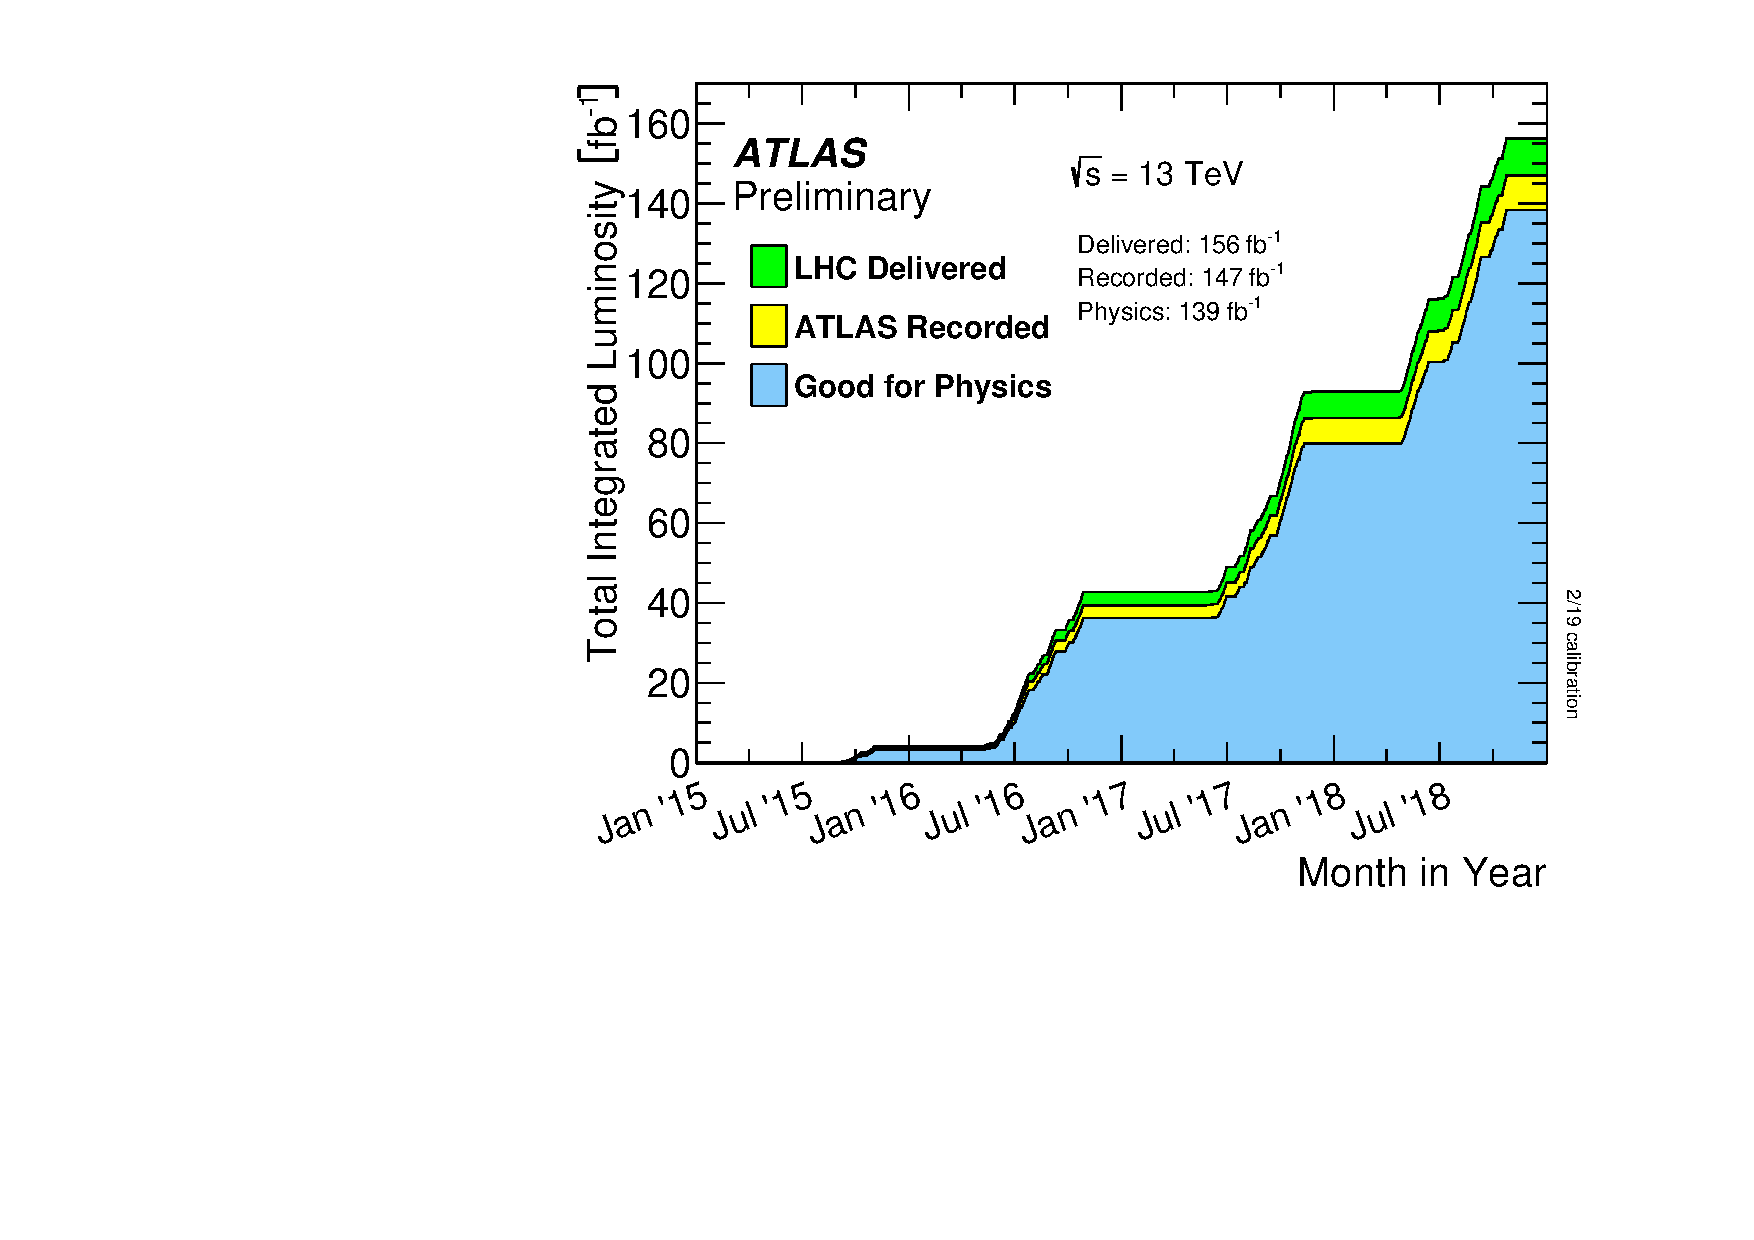
\includegraphics[width=0.75\textwidth]{figuresEXP/LHC2.pdf}
  \end{center}
  \caption{
  $Run\_2$计划期间LHC上质子-质子对撞数据的总积分亮度。
  到2018年底,LHC实现的数据总积分亮度为156$fb^{-1}$,
  ATLAS探测器所收集的数据总积分亮度为147$fb^{-1}$,
  在设备运转正常和数据采集稳定的情况下可用于实际物理分析的数据总积分亮度为139$fb^{-1}$。
  }
    \label{fig:LHC2}
\end{figure}

高能量和高密度的质子束流对撞为基本粒子的研究提供了可能。
LHC上有四个束流对撞点,每个对撞点都有一个实验,
共四个实验分别用于高能物理领域不同方面的研究:
%LHC上对应于束流四个碰撞点的四个实验分别用于研究基本粒子领域的不同方面:
其中ATLAS~\cite{PERF-2007-01}和CMS~\cite{CMS}是两个大型的通用型探测器,
用于标准模型的精确测量和寻找超出标准模型的新物理;
LHCb(Large Hadron Collider beauty)~\cite{LHCb}是一个用于研究B介子物理的正向探测器;
ALICE(A Large Ion Collider Experiment)~\cite{ALICE}是一个用于研究重离子碰撞的探测器。
%的研究着重于重离子碰撞。
其中ATLAS实验在$Run\_2$计划期间所收集的数据总积分亮度为147$fb^{-1}$,
在设备运转正常和数据采集稳定的情况下可用于实际物理分析的数据总积分亮度为139$fb^{-1}$。
%束流相交时非常高的质子-质子碰撞频率给探测器带来了极大的挑战,
%同时也因为高密度的质子束流使得两个单独的质子束相交时能够产生多次碰撞(堆积事例,pileup)~\cite{PileUp},让探测器中事例的重建也非常具有挑战性。
高频率的碰撞事例和高密度的质子束碰撞产生的堆积事例(Pileup)~\cite{PileUp}给探测器和其中事例的重建带来了极大的挑战。
%图~\ref{fig:LHC3}~的是ATLAS实验在$Run\_2$计划期间记录的质子束相交时发生碰撞的平均次数的简况图~\cite{ATLASWEB1}。
图~\ref{fig:LHC3}~展示的是ATLAS实验在$Run\_2$计划期间记录的每个质子束碰撞产生的平均事例数(Mean number of interactions per crossing)的分布图~\cite{ATLASWEB1}。
%质子束相交时发生碰撞的平均次数的简况图~\cite{ATLASWEB1}。
%总体来说,ATLAS实验在$Run\_2$计划期间收集的质子束相交时发生碰撞的平均次数为$\langle\mu\rangle=33.7$。
第~\ref{cha:Dijet}~章所介绍的物理分析所用到的数据便是ATLAS实验在$Run\_2$计划期间收集的,
接下来将对ATLAS实验做简要介绍。
%论文后面的物理分析所用到的数据便是由\textsc{ATLAS}实验在$Run\_2$计划期间收集的,下一部分将对ATLAS实验做更加详细的介绍。

\begin{figure}
  \begin{center}
    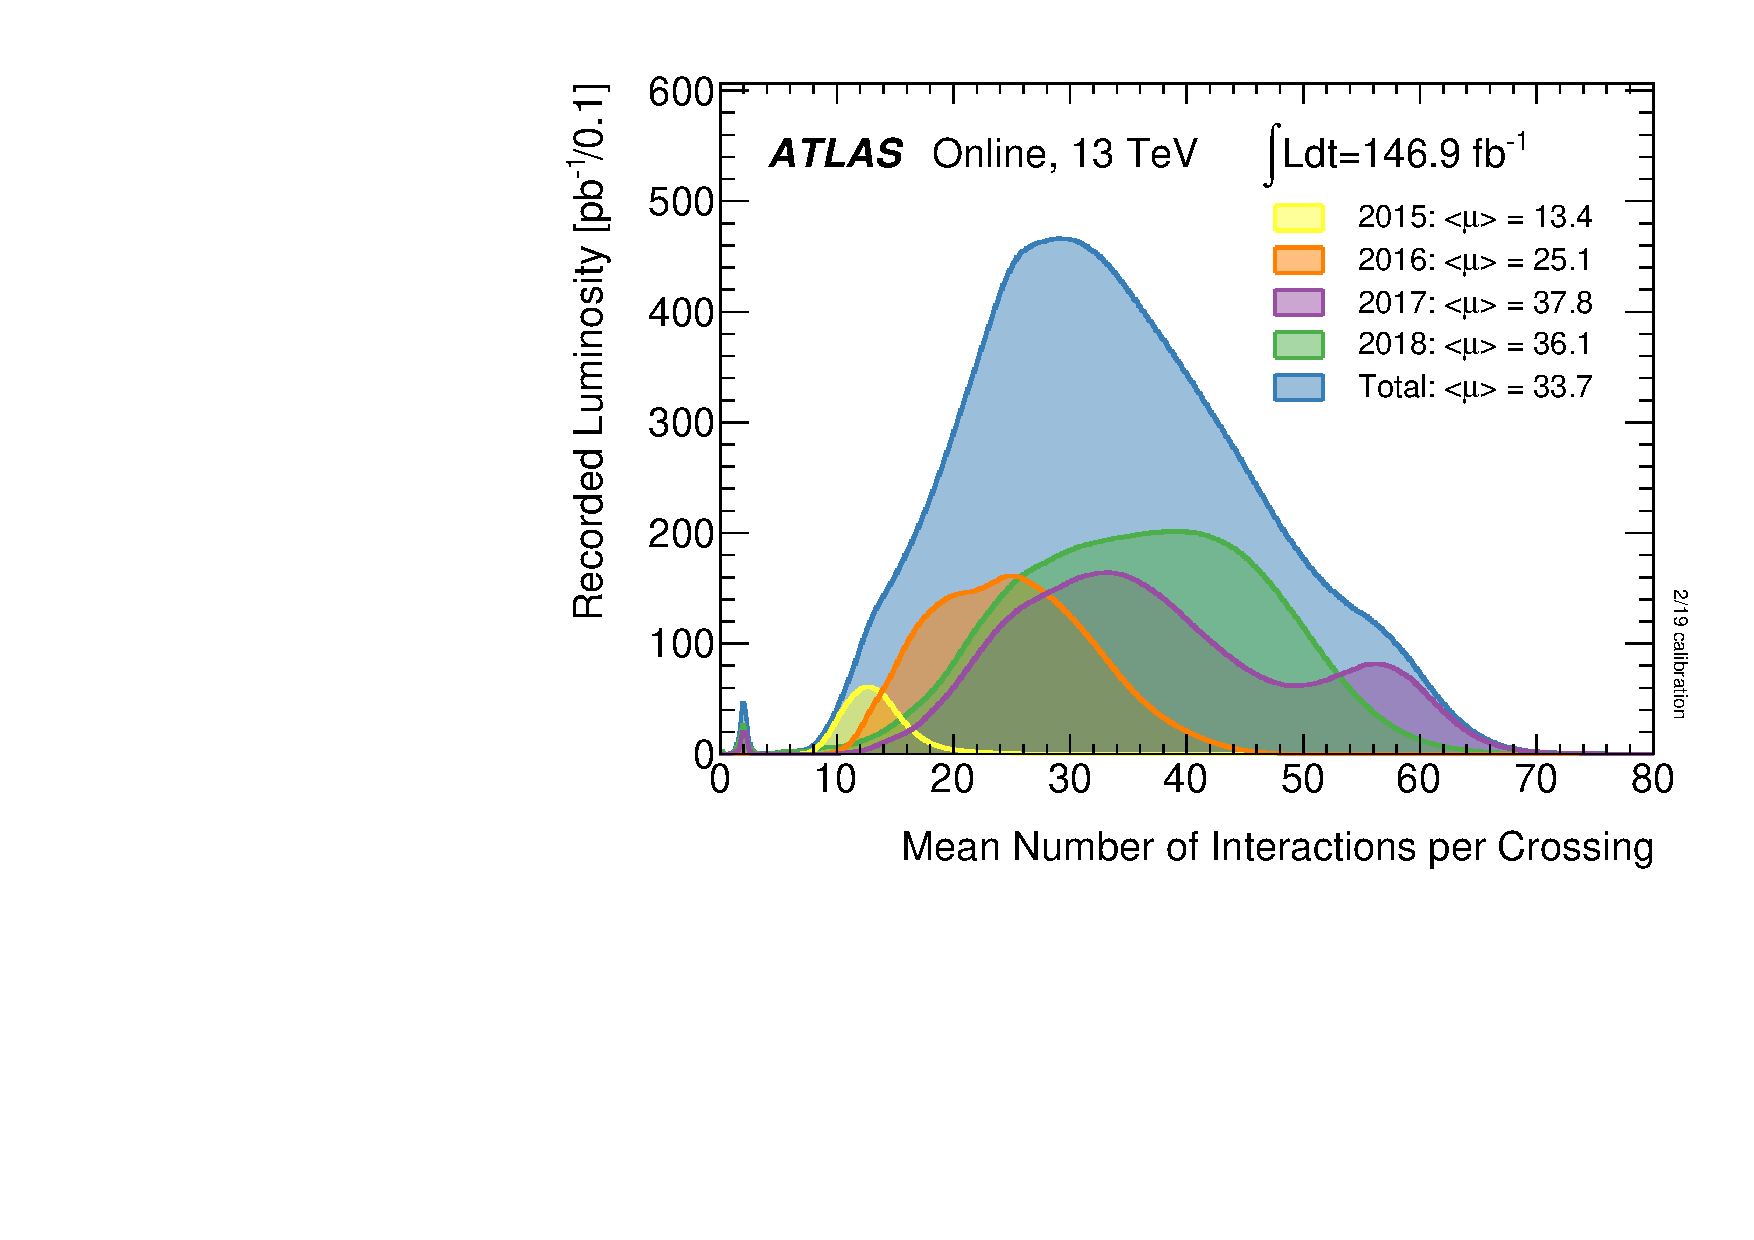
\includegraphics[width=0.75\textwidth]{figuresEXP/LHC3.pdf}
  \end{center}
  \caption{
  $Run\_2$计划期间ATLAS实验记录的每个质子束碰撞产生的平均事例数的分布图。
  %质子束相交时发生碰撞的平均次数。图示为四年中堆积事例的概况,
  在2017年的分布中有个两个峰值是因为年中LHC操作方案的调整。
    }
    \label{fig:LHC3}
\end{figure}


\section{ATLAS探测器}
\label{sec:ATLAS}

ATLAS(A Toroidal LHC ApparatuS)~\cite{PERF-2007-01,ATLASPERF1,ATLASPERF2}探测器是用于粒子物理研究的一个通用型探测器,
%通过它能观察到质子-质子对撞过程产生的所有衰变产物。
也是有史以来人类建造的体积最大的粒子探测器。
如图~\ref{fig:ATLAS1}~所示是探测器的一张截面图,它关于对撞点前后对称,其圆柱形桶身几乎覆盖了整个$4\pi$立体角。
整个探测器长44m,宽25m,重达7000吨,位于
%地下约100m处的
LHC其中一个质子-质子对撞点。

\begin{figure}
  \begin{center}
    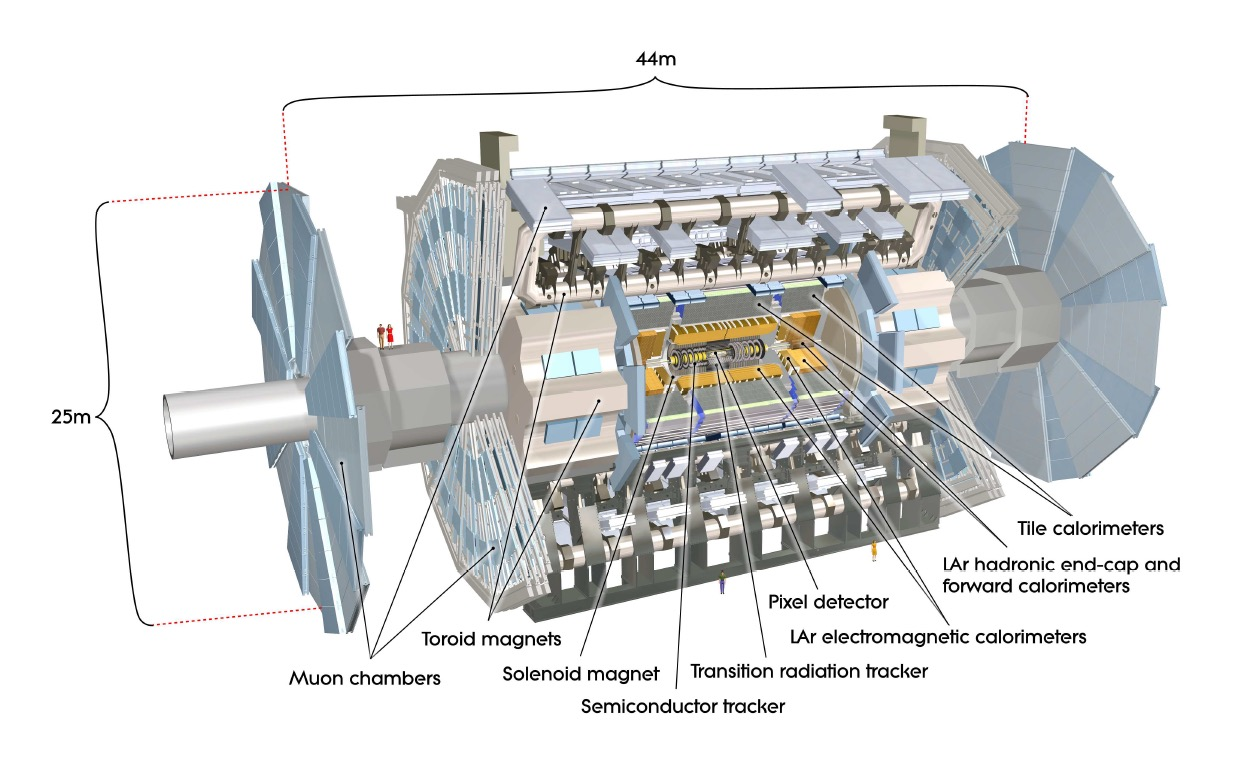
\includegraphics[width=0.75\textwidth]{figuresEXP/ATLAS1.jpg}
  \end{center}
  \caption{
ATLAS探测器的截面图。
  }
    \label{fig:ATLAS1}
\end{figure}

LHC上高亮度和高能量的质子束流对撞使得探索TeV能标的物理学成为可能,
其中ATLAS的设计初衷主要基于以下几个目标:
希格斯玻色子的寻找及其基本性质的测量;
量子色动力学、电弱相互作用、味物理等标准模型的精确测量;
超出标准模型的新物理的寻找,比如暗物质、新的重玻色子等;
t夸克性质的精确测量,比如质量、耦合常数和自旋等;
寻找超对称等标准模型的延拓理论。

%为了能处理约高达$6\times10^8s^{-1}$的质子-质子非弹性碰撞事例产生率,\textsc{ATLAS}探测器的设计需要满足几个条件:
为了处理高达约$6\times10^8s^{-1}$的事例产生率,探测器的设计需要满足以下几个条件:
抗辐照且高速的电子设备和传感器元件、高粒度的探测器材料,用于处理高通量的粒子和减小堆积事例带来的影响;
覆盖几乎整个$4\pi$立体角的高接收度;
%覆盖几乎整个方位角的高接收度;
能精确追踪带电粒子,要求具有高的动量分辨率,径迹重建效率和第二顶点重建效率等;
高粒度的电磁量能器和强子量能器,用于电子、光子和喷注等能量测量;
%精确的电磁量能技术和强子量能技术,用于电子、光子和喷注等能量测量;
能精确的识别$\mu$子和高的$\mu$子动量分辨率。
因此,ATLAS采用层叠式设计,从里到外由不同的子探测器组成,覆盖在束流管和对撞点周围,
它们依次是内部探测器(The Inner Detector, ID)~\cite{ATLASINNER}、电磁量能器(The Electromagnetic Calorimeter)、
强子量能器(The Hadronic Calorimeter)、前端量能器(The Forward Calorimeter)~\cite{ATLASLACA,ATLASTCA}、
$\mu$子谱仪(The Muon Spectrometer)~\cite{ATLASMUSPEC}和亮度探测器(The Luminosity Detectors)~\cite{ATLASLUMID}。
其中,内部探测器处于一个平行于束流轴的强度为2T的恒定磁场中,它可以测量带电粒子的运动方向、动量和电荷,也可以用来重建碰撞顶点。
量能器用来吸收光子、电子和强子并测量它们的能量,它能吸收除$\mu$子和中微子之外的所有已知粒子。
$\mu$子谱仪位于探测器的最外面,它也被包围在一个恒定的强磁场中,磁场由超导磁铁产生,使它能以非常高的精度测量$\mu$子的轨迹和动量。
三个亮度探测器位于ATLAS探测器前端
%依次是切伦科夫亮度探测器(the Luminosity measurement using Cerenkov Integrating Detector, LUCID)、零能探测器(the Zero-Degree Calorimeter, ZDC)和绝对亮度探测器(the Absolute Luminosity For ATLAS, ALFA)
,用来测量束流亮度。
表~\ref{tab:ATLASTab1}~总结了ATLAS的子探测器的主要性能目标。

\begin{table}[htbp]
      \caption{ATLAS的子探测器的主要性能目标。}
      \label{tab:ATLASTab1}
      \centering
      \begin{adjustbox}{width=\columnwidth,center}
      \begin{tabular}{|c|c|c|c|}
         \hline
         Detector component & Required resolution & \thead{$\eta$ coverage \\ (Measurements)} & \thead{$\eta$ coverage \\ (Trigger) } \\
        \hline
         Tracking & $\sigma_{p_{T}}/p_{T}=0.05\%/\sqrt{p_{T}}\oplus 0.01\%$  & $\pm2.5$ &  \\
        \hline
         EM calorimetry & $\sigma_{E}/E=10\%/\sqrt{E}\oplus 0.7\%$ & $\pm3.2$ & $\pm2.5$  \\
         \hline
         \thead{Hadronic calorimetry (jets) barrrel \\ and end-cap forward} & $\thead{\sigma_{E}/E=50\%/\sqrt{E}\oplus 3\% \\ \sigma_{E}/E=100\%/\sqrt{E}\oplus 10\%}$ & $\thead{\pm3.2 \\ 3.1<|\eta|<4.9}$ & $\thead{\pm3.2 \\ 3.1<|\eta|<4.9}$  \\
         \hline
         Muon spectrometer & $\sigma_{p_{T}}/p_{T}=10\% \quad at \quad p_{T}=1TeV$ & $\pm2.7$ & $\pm2.4$  \\
         \hline
      \end{tabular}
      \end{adjustbox}
\end{table}

%物理对象的重建是根据物理对象与探测器材料的相互作用实现的,如图~\ref{fig:ATLAS2}所示,是\textsc{ATLAS}探测器中鉴别和重建粒子的过程简图~\cite{ATLASTool}。
物理对象的重建是基于物理对象或者它们的衰变变产物与探测器材料的相互作用,
如图~\ref{fig:ATLAS2}~所示,展示的是ATLAS探测器中物理对象的鉴别和重建的过程简图~\cite{ATLASTool}。
带电粒子在ATLAS的内部探测器中会留下电离信息,以此来重建它的径迹,
%但是电中性的粒子比如说中微子不会,
其中的磁场会使带电粒子发生偏转,由此来重建它的动量和电荷。
除中微子之外,所有粒子都会在电磁量能器和强子量能器中沉积一部分或者全部的能量,
电磁量能器主要用于沉积光子和电子的能量,
强子量能器主要用于沉积强子的能量。
电子、光子、质子和中子等寿命较长的粒子会在量能器中产生一团簇射并停留在里面,
而$\mu$子会穿过内部探测器和量能器,在量能器中沉积一小部分能量之后,最终停在$\mu$子谱仪当中。
中微子因为其独特的性质不能被ATLAS探测到,
%重建过程中
可以通过事例中动量守恒来推断它们的存在。
接下来将对ATLAS的各个子探测器和物理对象的重建过程做更加详细的描述。

\begin{figure}
  \begin{center}
    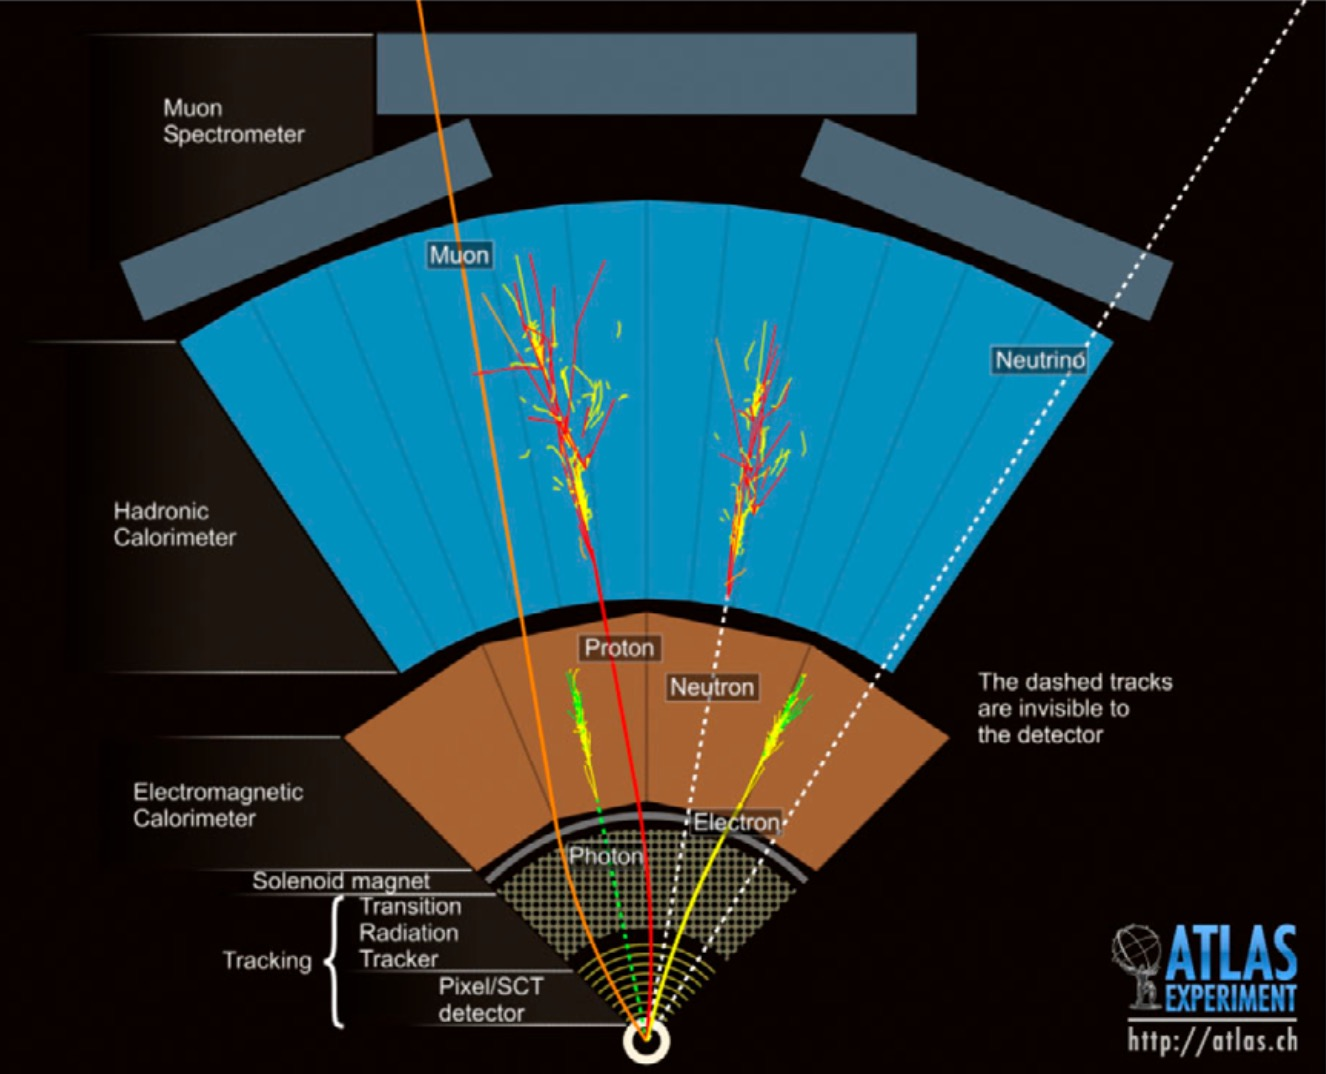
\includegraphics[width=0.75\textwidth]{figuresEXP/ATLAS2.jpg}
  \end{center}
  \caption{
  ATLAS探测器中物理对象的鉴别和重建的过程简图。
  }
    \label{fig:ATLAS2}
\end{figure}

\subsection{坐标系}
\label{sec:ATLASCS}

在ATLAS合作组所使用的坐标系中,
原点位于束流碰撞中心,
%原点位于质子-质子碰撞点,
$z$轴指向束流方向,$x$轴指向LHC大环的中心,
$y$轴垂直于$x$-$z$平面向上。
如图~\ref{fig:ATLAS3}~所示为ATLAS坐标系简图,$x$-$y$平面是束流的横截面。

\begin{figure}
  \begin{center}
    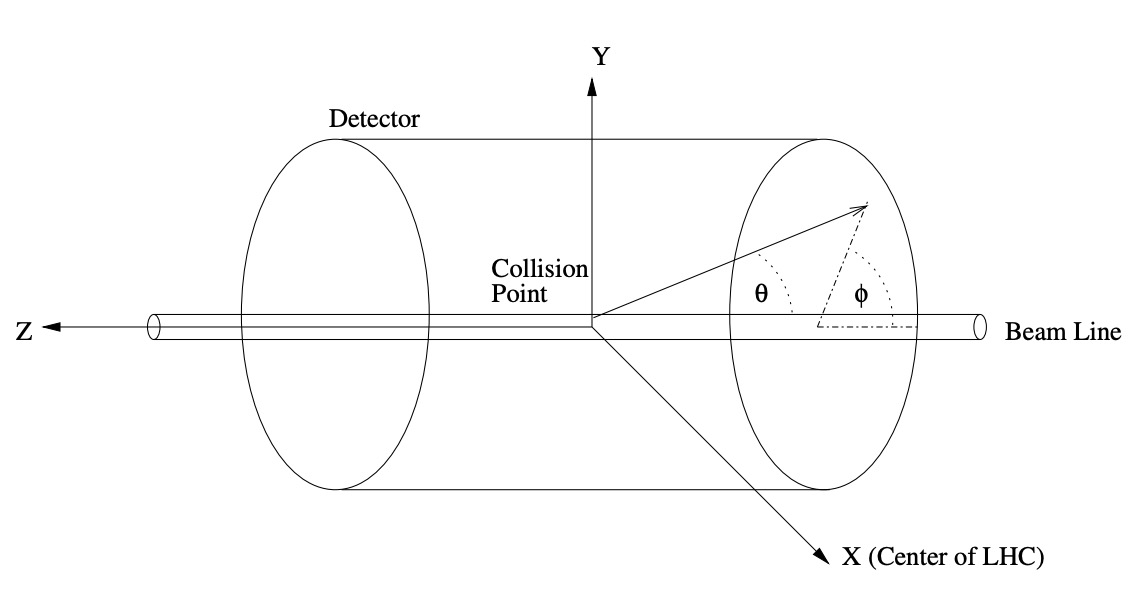
\includegraphics[width=0.75\textwidth]{figuresEXP/ATLAS3.jpg}
  \end{center}
  \caption{
ATLAS合作组所使用的坐标系。
  }
    \label{fig:ATLAS3}
\end{figure}

根据ATLAS探测器的对称性,也可以使用柱坐标系$(R,\phi,\theta)$,
其中$R=\sqrt{x^2+y^2}$,$\theta$是粒子与z轴所形成的极角,
$\phi$是粒子绕z轴的方位角。
这里引入快度$y$,定义为:
\begin{equation} 
\label{eq:ydef}
y=\frac{1}{2}ln\left( \frac{E+p_{z}}{E-p_{z}} \right)
\end{equation}
其中$E$和$p_{z}$分别是粒子的能量和粒子的动量沿z轴方向的分量。
可以证明$\Delta y$在沿z轴方向的洛伦兹变换下是不变的。
如果粒子的质量相对于粒子的能量可以忽略不计,
那么快度$y$可以近似成赝快度$\eta$:
\begin{equation} 
\label{eq:etadef}
\eta=-ln\left(\tan\frac{\theta}{2} \right)
\end{equation}
其中$\theta$为极角,
$\eta$是高能物理领域中描述粒子极角的常用空间坐标,
图~\ref{fig:ATLAS4}~展示了坐标平面中不同的$\eta$值所对应的$\theta$值。
%横动量$p_{T}=\sqrt{p_x^2+p_y^2}$和横能量$E_{T}=E\sin\theta$分别定义为粒子沿$x$-$y$平面的动量和能量。
横动量$p_{T}=\sqrt{p_x^2+p_y^2}$是粒子沿$x$-$y$平面的动量。
$\Delta R$定义为粒子在$\eta$-$\phi$空间的距离:
\begin{equation} 
\label{eq:DRdef}
\Delta R=\sqrt{\Delta\eta^2+\Delta\phi^2}
\end{equation}
其中$\Delta\eta$和$\Delta\phi$分别为粒子的赝快度$\eta$之差和方位角$\phi$之差。

\begin{figure}
  \begin{center}
    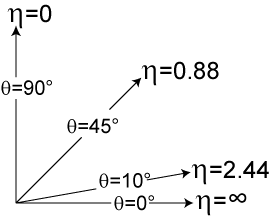
\includegraphics[width=0.5\textwidth]{figuresEXP/ATLAS4.png}
  \end{center}
  \caption{
坐标平面中不同的赝快度$\eta$所对应的极角$\theta$。
%赝快度$\eta$和所对应的极角$\theta$值。
  }
    \label{fig:ATLAS4}
\end{figure}


\subsection{磁系统}
\label{sec:ATLASMS}

为了精确地重建带电粒子的径迹以及测量带电粒子的动量和电荷,探测器需要一个非常强的磁场。
当一个动量为p、带电量为q的粒子垂直进入一个强度为B的磁场时,
在洛伦兹力的作用下,粒子会做圆周运动,运动的曲率半径$\rho$为:
\begin{equation} 
\label{eq:rhodef}
\rho=\frac{p}{q\cdot B}
\end{equation}
因此,为了确定带电粒子的动量,
需要测量其通过探测器中磁场时的曲率半径。
%需要测量其通过磁场中探测器时轨迹的曲率半径。
如图~\ref{fig:ATLAS5}~所示,
%ATLAS探测器中包含两个由以下四个大型的超导磁体提供的独立磁系统~\cite{ATLASMS}:
ATLAS探测器中包含两个独立的磁系统~\cite{ATLASMS},由以下四个大型超导磁体提供:
位于内部探测器和电磁量能器之间的中心螺线管(The Central Solenoid, CS),
它与z轴对齐,直径为2.4m,长5.3m,
能为内部探测器提供一个强度为2T的轴向磁场,同时能减小桶部电磁量能器前端的辐射厚度;
25m长的桶部环形磁体(The Barrel Toroid, BT)和两组5m长的端盖环形磁体(The End-Cap Toroids, ECT),
%它们能为$\mu$子谱仪提供一个与$\mu$子轨迹接近垂直的强度为4T的环形磁场。
它们能为$\mu$子谱仪提供一个强度为4T的环形磁场,磁场方向与$\mu$子轨迹接近垂直。
%整个磁系统置于在温度为4.8K的液氦中。

\begin{figure}
  \begin{center}
    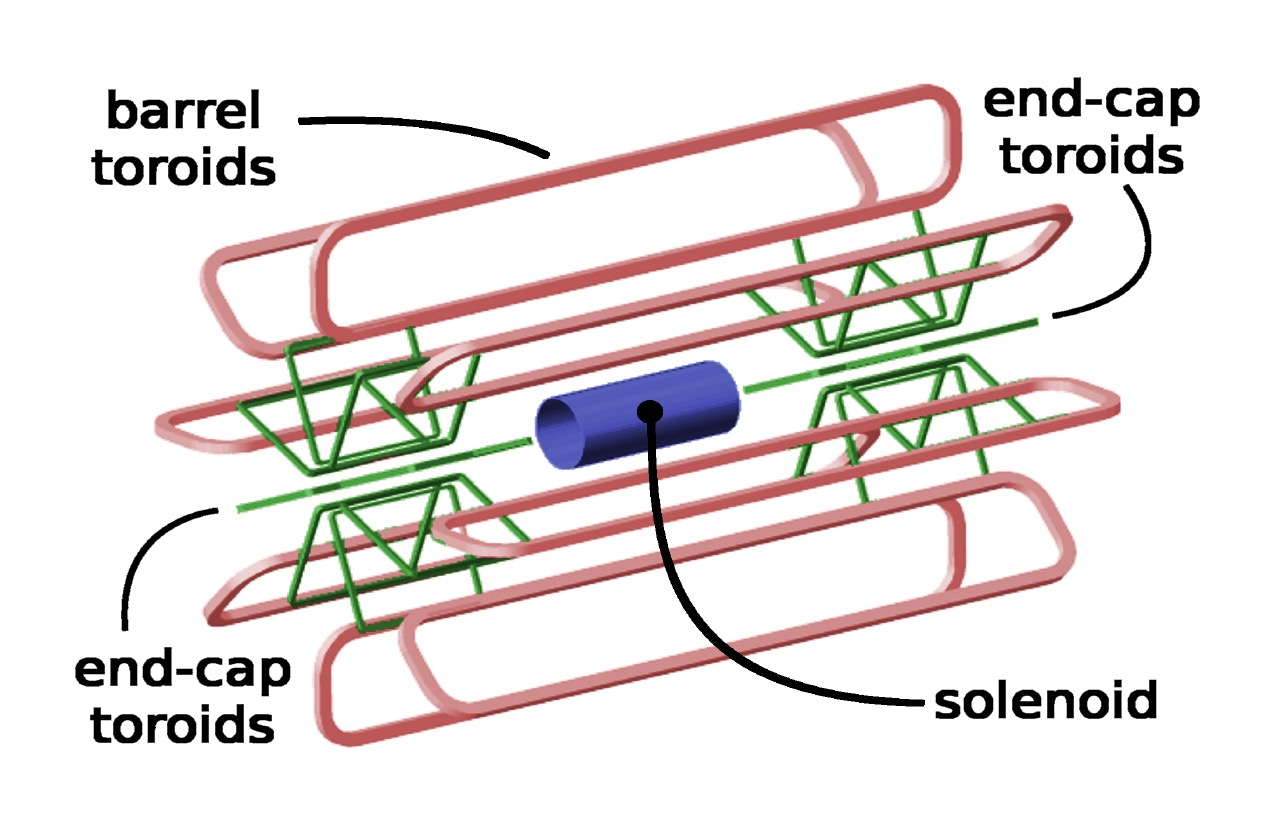
\includegraphics[width=0.75\textwidth]{figuresEXP/ATLAS5.jpg}
  \end{center}
  \caption{
 ATLAS探测器的磁系统布局。
 %\textsc{ATLAS}探测器中磁系统的布局。
  }
    \label{fig:ATLAS5}
\end{figure}

\subsection{内部探测器}
\label{sec:ATLASID}

如图~\ref{fig:ATLAS6}~所示,是ATLAS内部探测器(The Inner Detector, ID)的截面图,
它是由桶部和端盖部分同心的多层探测材料组成,离对撞点最近,
长6.2m,端盖半径为1.1.m,处于一个强度为2T的螺线管磁场中。
主要用于高精度的重建带电粒子的动量、径迹和事例的主顶点、第二顶点等信息,覆盖了$|\eta|<2.5$的范围。
%它长6.2m,端盖半径为1.1.m,并处于一个强度为2T的螺线管磁场中。

\begin{figure}
  \begin{center}
    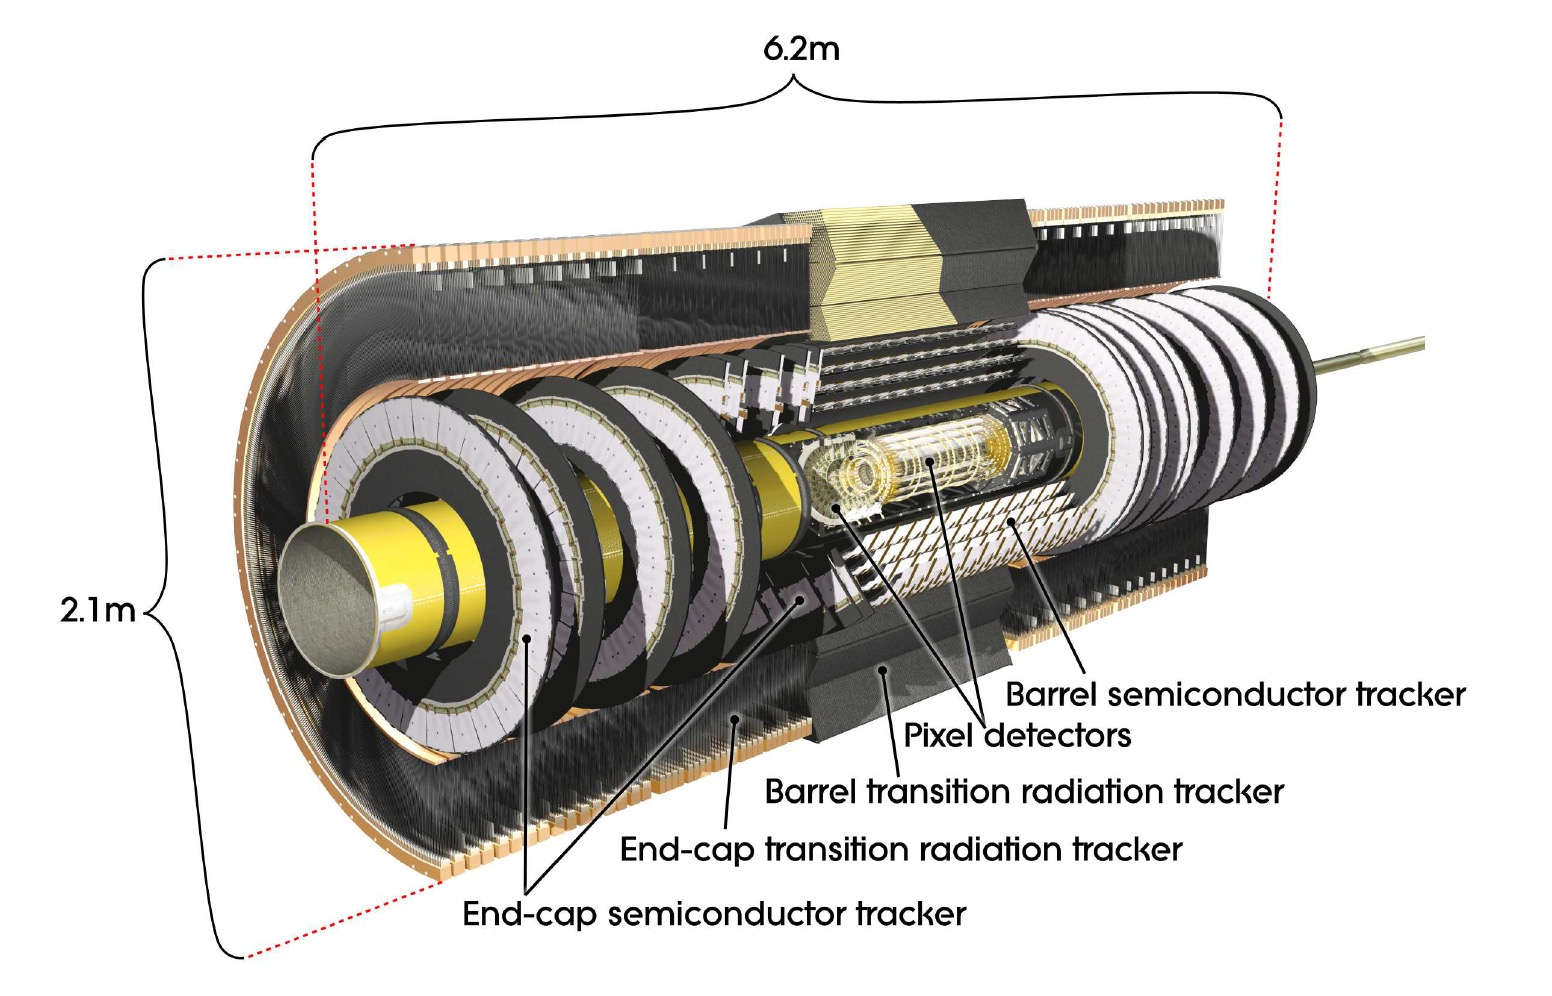
\includegraphics[width=0.75\textwidth]{figuresEXP/ATLAS6.jpg}
  \end{center}
  \caption{
ATLAS内部探测器的截面图和它的子结构。
  }
    \label{fig:ATLAS6}
\end{figure}

为了实现高精度的径迹和顶点重建,
它是由四个高粒度且功能互补的子探测器组成,
如图~\ref{fig:ATLAS7}~,从里到外,%从最里层到最外层,
依次是嵌入式B层探测器、像素探测器、半导体径迹探测器和跃迁辐射径迹探测器。

\begin{figure}
  \begin{center}
    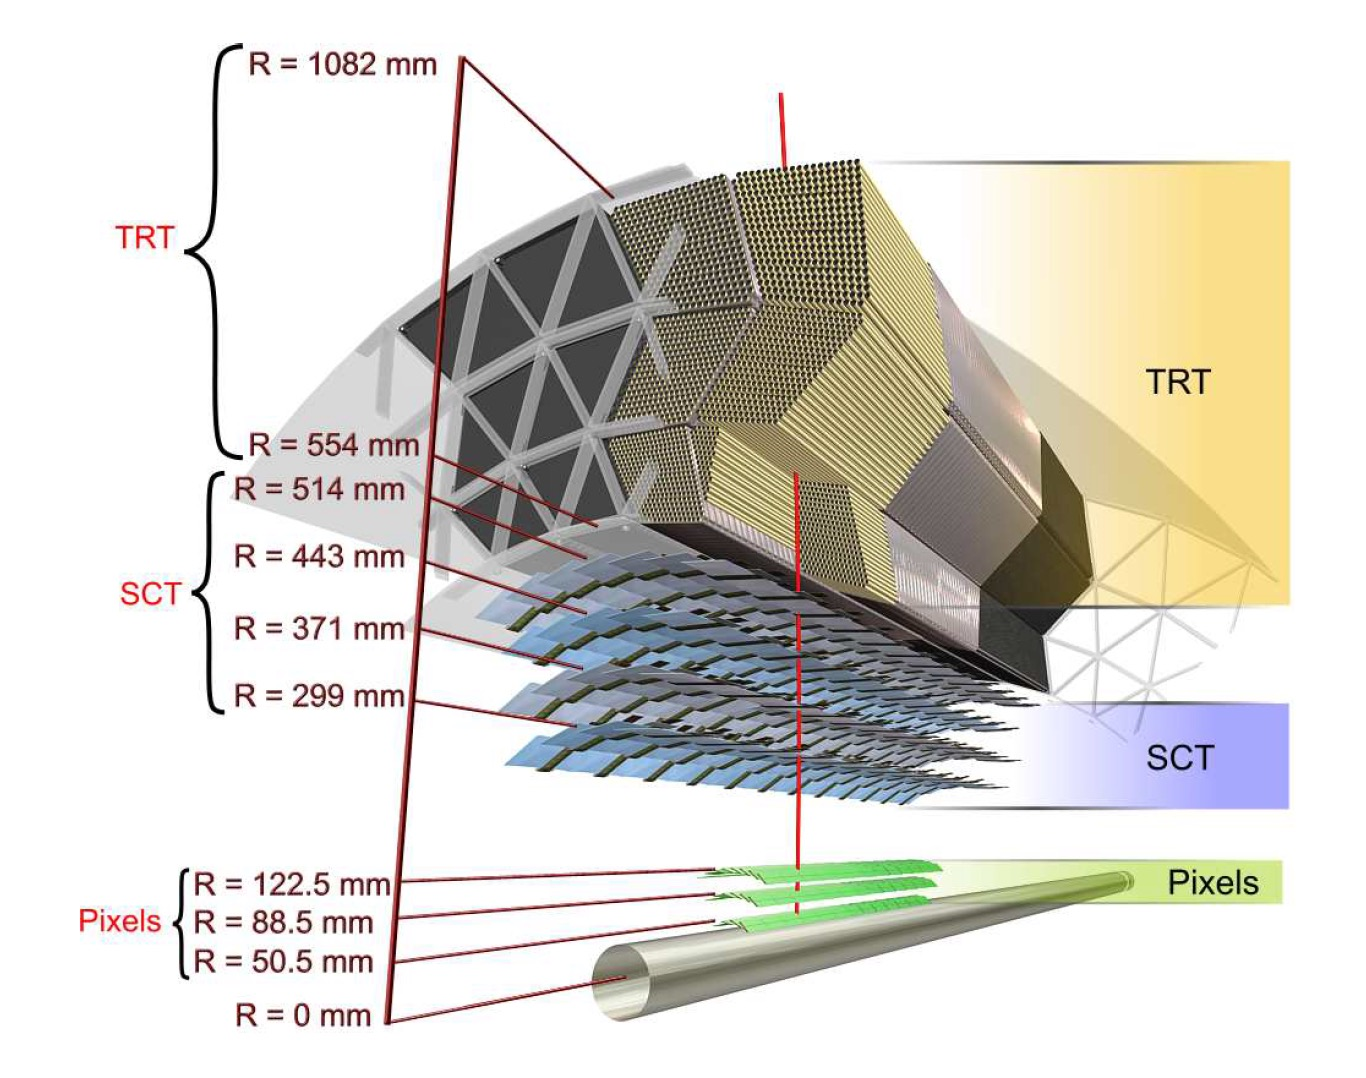
\includegraphics[width=0.75\textwidth]{figuresEXP/ATLAS7.jpg}
  \end{center}
  \caption{
ATLAS内部探测器的桶部截面图。灰色的小圆柱是LHC的束流管。
%嵌入式B层探测器是在$Run\_2$计划期间安装的。
%ATLAS内部探测器的桶部子探测器的截面简图。灰色的小圆柱是LHC的束流管。嵌入式B层探测器(LBL)是在$Run\_2$计划期间安装的。
  }
    \label{fig:ATLAS7}
\end{figure}

嵌入式B层探测器(The Insertable B-Layer, IBL)~\cite{ATLASIBL}是内部探测器中离束流管最近的一个子探测器。
$Run\_2$计划所面临的其中一个重要问题是总积分亮度的显著增加会给内部探测器带来很大的辐照损伤,
%$Run\_2$计划面临的主要问题之一是总积分亮度的显著增加会给内部探测器带来很大的辐照损伤,
进而会导致内部探测器的径迹重建效率下降,尤其是b-jet的重建效率。
嵌入式B层探测器正是在这样的背景之下安装到ATLAS内部探测器中的,%它是在$Run\_2$计划执行之前安装的,
%嵌入式B层探测器正是在这样一个背景下加入到ATLAS的内部探测器中的,它是在$Run\_2$计划执行之前安装的,
它呈柱状,半径33.2mm,长3.5m,覆盖在束流管外面。
%位于铍制束流管和像素探测器的第一层之间。
%为了处理束流的高亮度,
它不仅抗辐照,而且
%其中的
每个像素传感器单元的尺寸都很小,仅有50$\mu m$×250$\mu m$($R$-$\phi\times z$),
固有精度是8$\mu m$($R$-$\phi$)和40$\mu m$($z$),覆盖了
%整个
$0\le\phi<2\pi$的范围。
嵌入式B层探测器对测量精确的提升非常显著,
图~\ref{fig:ATLAS8}~展示是碰撞参数$d_0$的分辨率
%变化曲线
的前后对比图,
%其中碰撞参数$d_0$定义为$x$-$y$平面上径迹中离$z$轴最近的点与$z$轴之间的距离,
其中碰撞参数$d_0$是带电粒子的径迹在$x$-$y$平面上的投影离主顶点最短的距离,
它是影响b-jet标定性能的关键参数。
%除了碰撞参数的分辨率,嵌入式B层探测器对顶点重建效率和b-jet标定性能~\cite{IBLBP}也有明显的提升。
除此之外,嵌入式B层探测器也会显著的提升顶点重建效率和b-jet标定性能~\cite{IBLBP}。
%这些提升主要是因为嵌入式B层探测器相对于像素探测器更靠近束流并能分辨更小的尺度。

\begin{figure}
  \begin{center}
    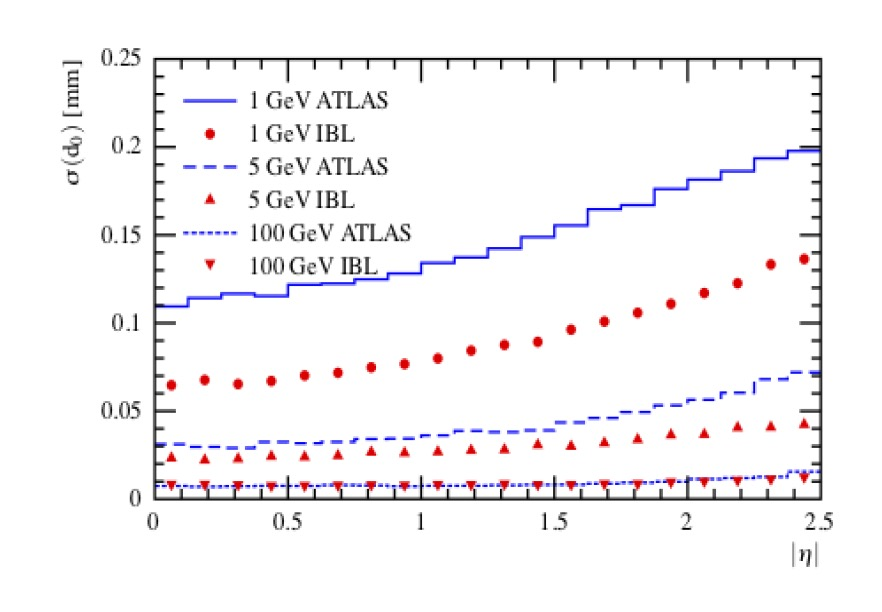
\includegraphics[width=0.75\textwidth]{figuresEXP/ATLAS8.jpg}
  \end{center}
  \caption{
 ATLAS内部探测器中安装和未安装嵌入式B层探测器(IBL)的情况下,
 %单
 $\mu$子碰撞参数$d_0$的分辨率随着赝快度$\eta$的变化关系对比。
  }
    \label{fig:ATLAS8}
\end{figure}

像素探测器(The Pixel Detector, PD)为对撞点附近的模式识别提供关键的径迹信息。
如图~\ref{fig:ATLAS9}~所示,
%它是由三个分别位于以束流轴为中心的半径为51mm、89mm和123mm处的桶层结构和左右两边两个端盖结构组成,
它是由三个桶层结构和左右两个端盖结构组成,
其中桶层结构分别位于以z轴为中心的半径51mm、89mm和123mm处,
%其中
每个端盖具有三个圆盘层,分别位于$|z|$=495mm、$|z|$=580mm和$|z|$=650mm处。
端盖和桶层结构中硅像素传感器~\cite{PDSS}的尺寸都是50$\mu m$×400$\mu m$($R$-$\phi\times z$),
固有精度为10$\mu m$($R$-$\phi$)和115$\mu m$($z$)。
像素探测器能为$|\eta|<2.5$、$0\le\phi<2\pi$范围内的
%径迹提供三个或者更多个精确测量点。
带电粒子提供三个或者更多个径迹测量点,
%端盖和桶层结构中硅像素传感器~\cite{PDSS}的尺寸都是50$\mu m$×400$\mu m$($R$-$\phi\times z$),
%固有精度都为10$\mu m$($R$-$\phi$)和115$\mu m$($z$)。
%整个像素探测器
总共有大约80万个读出信道。
%$R$-$\phi$平面和沿束流轴方向的高分辨率对于精确重建动量、径迹、主顶点和第二顶点来说起着至关重要的作用。
它在粒子动量测量、径迹重建和事例的主顶点、第二顶点的重建中起着至关重要的作用。

\begin{figure}
  \begin{center}
    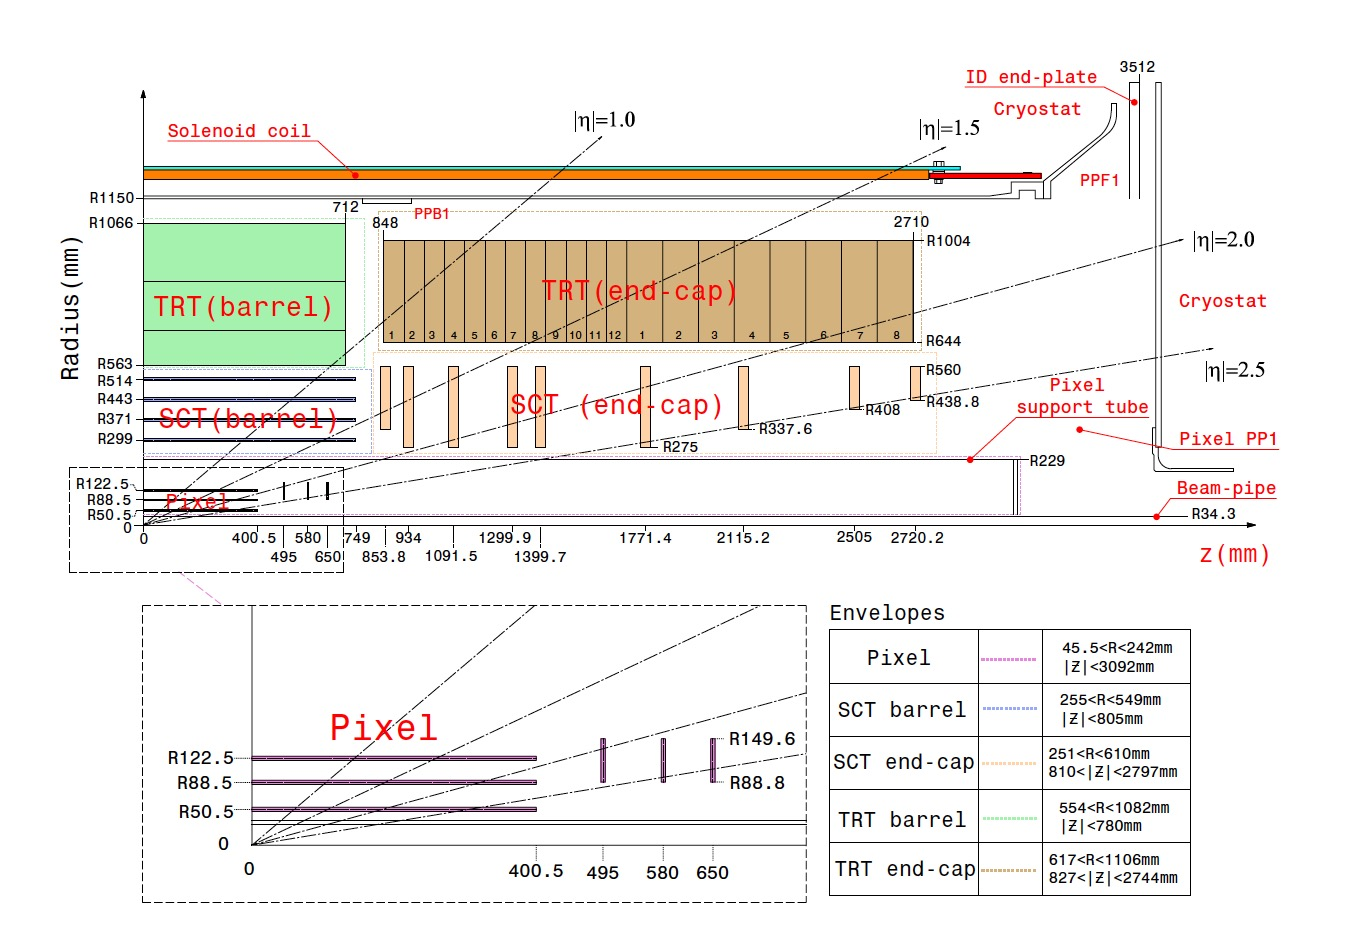
\includegraphics[width=0.75\textwidth]{figuresEXP/ATLAS9.jpg}
  \end{center}
  \caption{
ATLAS内部探测器沿$R$-$z$平面的截面图。图中展示了其中各个子探测器的位置、结构和尺寸等,左下部分是像素探测器的放大图。
  }
    \label{fig:ATLAS9}
\end{figure}

半导体径迹探测器(The SemiConductor Tracker, SCT)位于内部探测器的中间位置,采用了与像素探测器相同的半导体技术。
%并使用尺寸为120mm$\times$60mm($\phi\times z$)的硅微条~\cite{SCTSS}作为测量元件,同样覆盖了$|\eta|<2.5$、$0\le\phi<2\pi$的范围。
它使用尺寸为120mm$\times$60mm($\phi\times z$)的硅微条~\cite{SCTSS}作为测量元件,覆盖了$|\eta|<2.5$、$0\le\phi<2\pi$的范围。
如图~\ref{fig:ATLAS9}~所示,它是由四个桶层结构
%(299mm<$R$<514mm)
和左右两个
%各含九个圆盘层的
端盖结构
%(850mm<$z$<2730mm)
组成,
%其中四个分别由两层传感器构成的桶层结构位于以束流轴为中心的半径为30cm、37cm、44cm和51cm处。
其中四个桶层结构分别位于以束流轴为中心的半径30cm、37cm、44cm和51cm处,每个桶层结构由两层传感器组成,
每个端盖结构具有九个圆盘层,位于850mm<$z$<2730mm的区域,
端盖和桶层结构的固有精度都是17$\mu m$($R$-$\phi$)和580$\mu m$($z$)。
整个半导体径迹探测器共有6.3万个读出信道,
能在$R$坐标和$z$坐标上为
带电粒子提供四个额外的径迹测量点,
%每条径迹提供四个额外的空间测量点。
它的测量精度略低于像素探测器的精度,
%的测量精度,但是在重建动量、径迹和顶点方面仍发挥着重要作用。
但在粒子动量测量、径迹重建和事例的主顶点、第二顶点的重建中仍发挥着重要的作用。

跃迁辐射径迹探测器(The Transition Radiation Tracker, TRT)位于内部探测器的最外层,
它是一个组合型探测器~\cite{ATLASTRT},
一方面有径迹探测的功能,可以将内部探测器的径迹追踪能力扩展到径向大约1m处的位置,
也能像漂移室那样测量带电粒子的漂移时间;
另一方面可以作为跃迁辐射探测器用于模式识别,区分轻粒子和重粒子,比如利用电磁辐射区分电子和$\pi$介子。
%构成跃迁辐射径迹探测器的
其组件元是一个直径为4mm、长度为144mm的聚酰胺细管,
在每个细管中心,有一根直径为31$\mu m$的钨丝作为阳极连接到前段电子设备,
管壁和金属丝之间被$Xe$、$O_2$、$CO_2$混合气体填充,
当带电粒子使混合气体电离时,电子会向金属丝漂移,并在阳极触发一个低振幅的电信号。
而且由于介质的不均匀性,带电粒子在穿过聚酰胺管壁和混合气体的交界处时,会发生跃迁辐射,
辐射出来的光子会被混合气体中Xe吸收,Xe退激发时会在阳极触发一个高振幅的电信号,
可以与气体电离触发的低振幅电信号区分开。

\subsection{量能器}
\label{sec:ATLASCA}

如图~\ref{fig:ATLASCA1}~所示,ATLAS的量能器系统~\cite{ATLASLACA,ATLASTCA}包围在内部探测器的外面,
覆盖了整个$0\le\phi<2\pi$的范围。
它主要由电磁量能器(The Electromagnetic Calorimeter, ECal)、
强子量能器(The Hadronic Calorimeter, HCal)和前端量能器(The Forward Calorimeter, FCal)三大部分组成,
分别覆盖了$|\eta|<3.2$、$|\eta|<3.9$和$3.1<|\eta|<4.9$的范围。
整个量能器系统处于桶部和左右端盖处三个低温恒温箱中,
%并覆盖了整个$0\le\phi<2\pi$的范围。
%高能粒子通过与量能器中致密物质相互作用而产生很多次级粒子,
高能粒子在与量能器中致密物质相互作用时会产生很多次级粒子,
并且数量沿着入射粒子的方向成指数型增长,同时粒子的能量越来越低,最终停留在量能器中,
这个过程称为簇射~\cite{CABOOK}。
量能器便是通过高能粒子形成的簇射来测量其能量,
其中电磁量能器和前端量能器的电磁测量部分用于测量电子和光子
因电磁簇射而沉积的能量,
%因电磁相互作用形成簇射而沉积的能量,
强子量能器和前端量能器的强子测量部分用于测量强子
因强子簇射而沉积的能量。
%因强相互作用形成簇射而沉积的能量。

\begin{figure}
  \begin{center}
    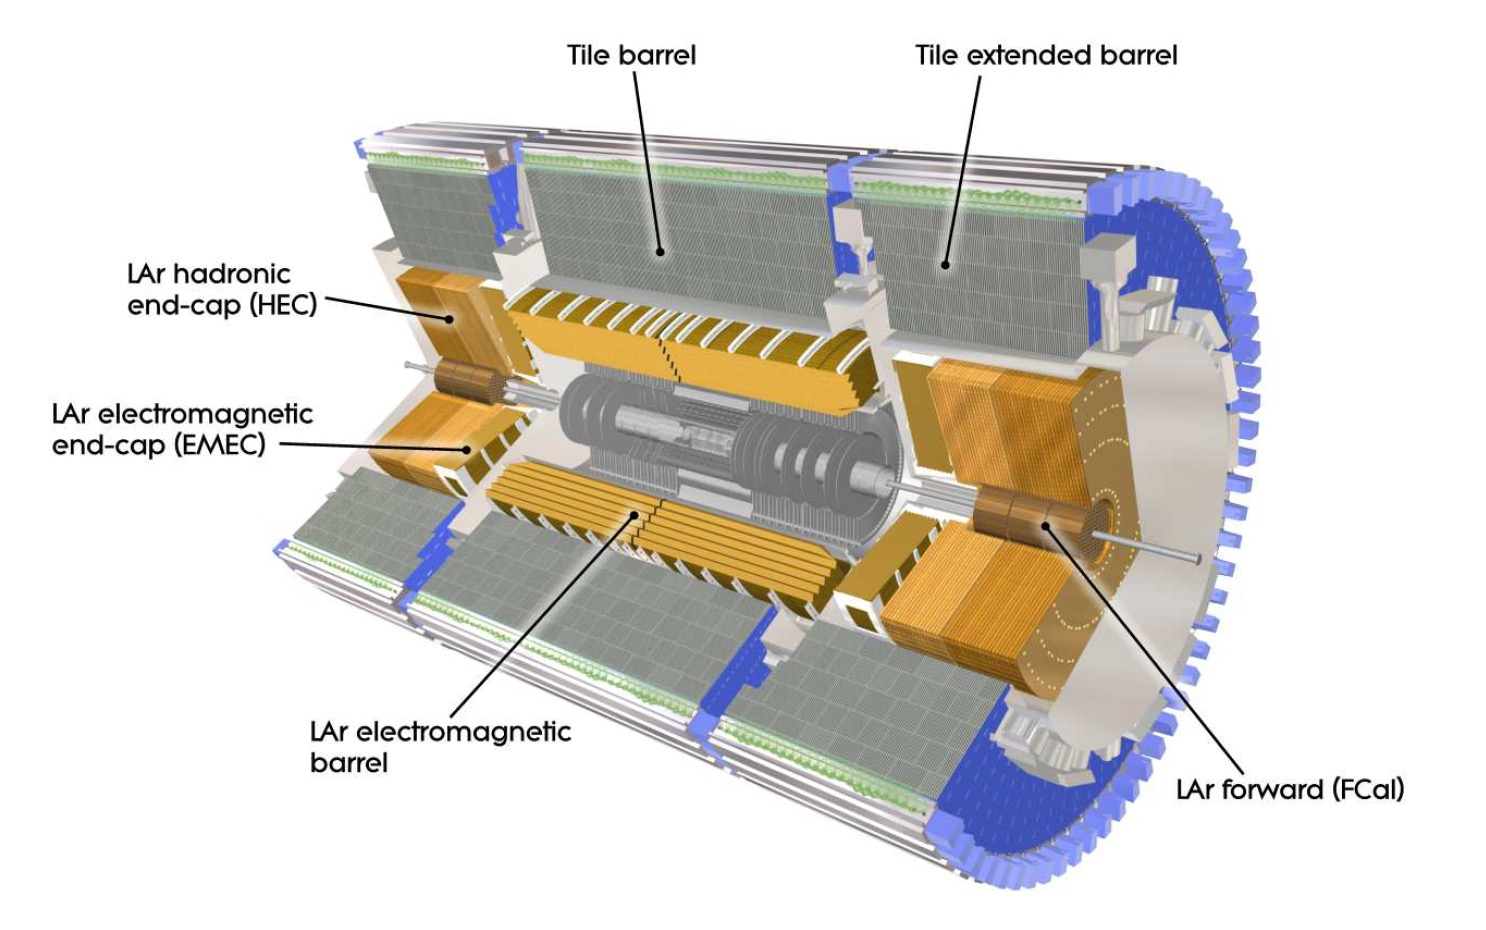
\includegraphics[width=0.75\textwidth]{figuresEXP/ATLASCA1.jpg}
  \end{center}
  \caption{
ATLAS的量能器系统的截面图。
  }
    \label{fig:ATLASCA1}
\end{figure}

ATLAS的量能器系统使用的是采样式量能器,
如图~\ref{fig:ATLASCA2}~所示,它们由吸收材料和活性材料交替组成。
其中吸收材料由铅、铜或者铁制成,用来降低入射粒子的能量,
液氩或者乙烯闪烁体用作活性材料,
活性材料与高能粒子相互作用能产生电离或者闪烁并形成可测量的信号,
%通过电离或者闪烁收集可测量的信号,
然后利用测量的小部分能量可以推断出完整的簇射能量。

\begin{figure}
  \begin{center}
    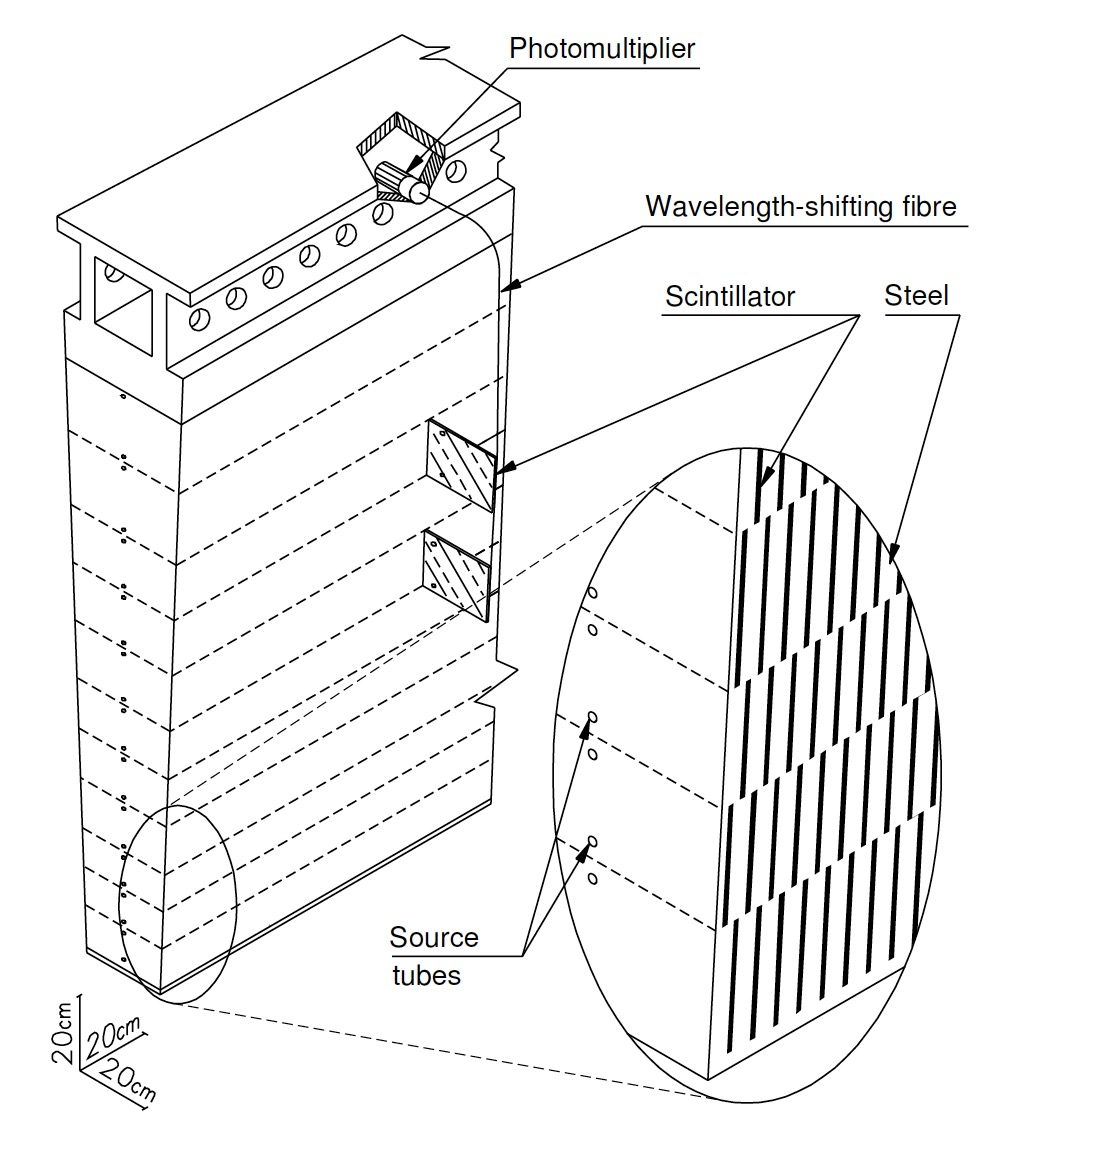
\includegraphics[width=0.75\textwidth]{figuresEXP/ATLASCA2.jpg}
  \end{center}
  \caption{
ATLAS量能器系统所使用的采样式量能器。
它们由吸收材料和活性材料交替组成,可测量信号由活性材料与高能粒子的相互作用形成。
%ATLAS的量能器的机械组件和读出系统的组装模式。
  }
    \label{fig:ATLASCA2}
\end{figure}

电磁量能器长6.65m,外径为2.25m,
分别由铅和液氩作为吸收材料和活性材料,
%聚酰亚胺薄膜电极用于信号输出,
其能量分辨率为:
\begin{equation} 
\label{eq:EMsigma1}
\frac{\sigma(E)}{E}=\frac{10\%}{\sqrt{E}}\oplus 0.7\%
\end{equation}
覆盖整个方位角$0\le\phi<2\pi$。
它可以分为桶部和左右端盖三部分,分别覆盖了$|\eta|<1.475$和$1.375<|\eta|<3.2$的范围。
为了能够完全的吸收入射电子和光子产生电磁簇射,
桶部和端盖的厚度分别大于22$X_0$和24$X_0$,
其中$X_0$为辐射长度,定义为粒子在其能量减小到初始能量的$1/e$时所经过的平均距离,
它可以用原子序数$Z$和原子质量数$A$近似的表示成~\cite{PDG}:
\begin{equation} 
\label{eq:X0def}
X_0=\frac{716.4A}{Z(Z+1)\ln(287/\sqrt{Z})}g cm^{-2}
\end{equation}
图~\ref{fig:ATLASCA3}~是桶部电磁量能器的模块示意图,
其中靠对撞点最近的第一层粒度较小,用于电子和光子的识别,
后面两层粒度较大,以保证电子和光子产生的电磁簇射能被完全吸收,
各部分在$\eta$和$\phi$方向的粒度也显示在图中。

\begin{figure}
  \begin{center}
    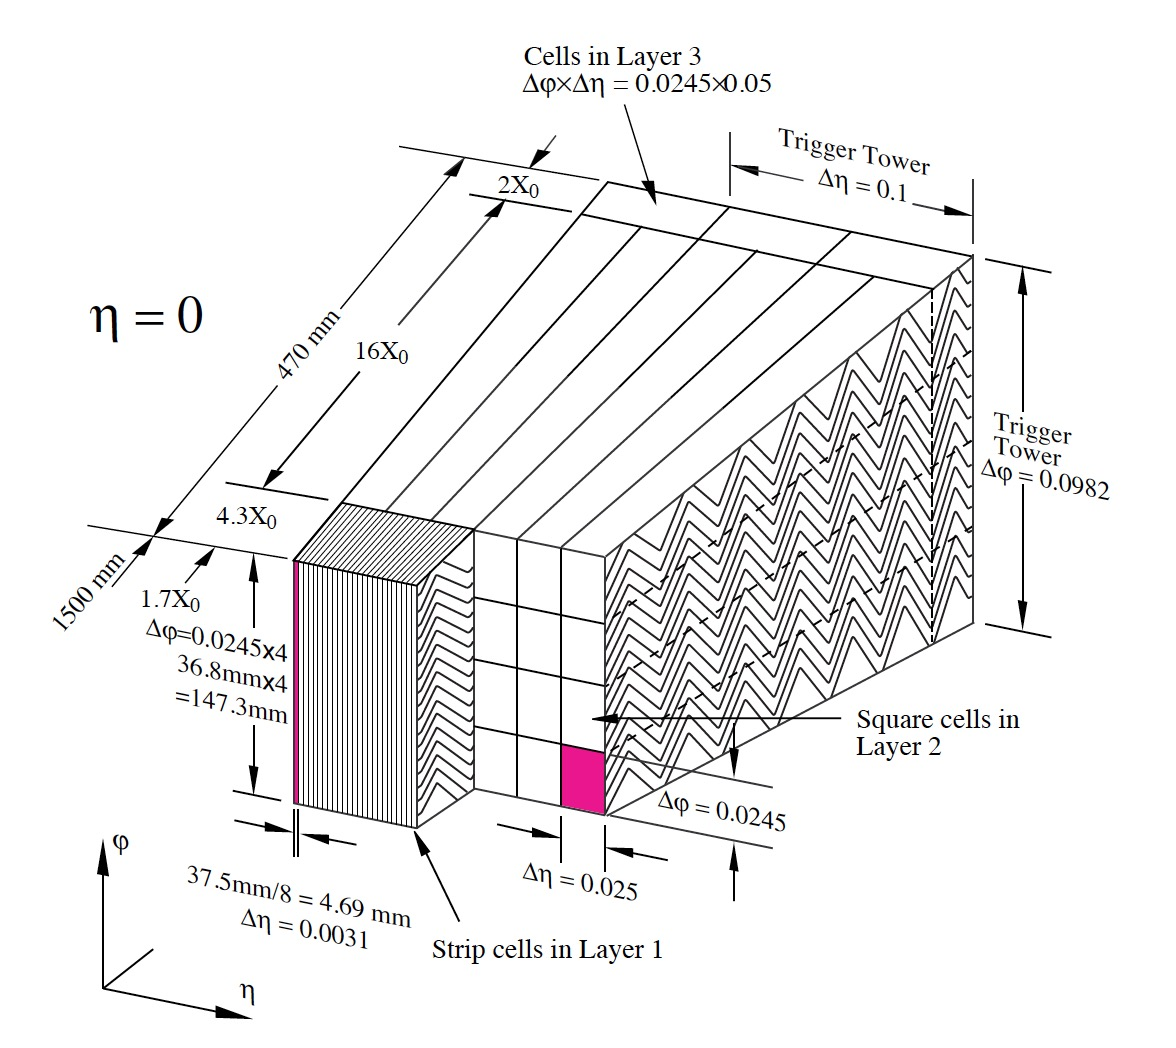
\includegraphics[width=0.75\textwidth]{figuresEXP/ATLASCA3.jpg}
  \end{center}
  \caption{
ATLAS桶部电磁量能器的模块示意图。
其中$X_0$为辐射长度,定义为粒子在其能量减小到初始能量的$1/e$时所经过的平均距离。
各部分在$\eta$和$\phi$方向的粒度也显示在图中。
  }
    \label{fig:ATLASCA3}
\end{figure}

强子量能器紧靠在电磁量能器外面,长6.10m,外径4.25m,
其能量分辨率为:
\begin{equation} 
\label{eq:EMsigma2}
\frac{\sigma(E)}{E}=\frac{50\%}{\sqrt{E}}\oplus 3\%
\end{equation}
同样由桶部和左右端盖三部分组成。
桶部强子量能器分别用铁和闪烁体作为吸收材料和活性材料,
粒度为$\Delta\eta\times\Delta\phi=0.1\times0.1$,
覆盖了$|\eta|<1.7$的部分。
端盖强子量能器分别用铜和液氩作为吸收材料和活性材料,
粒度随着$\eta$变化,在$1.5<|\eta|<2.5$的范围为$\Delta\eta\times\Delta\phi=0.1\times0.1$
,在$2.5<|\eta|<3.2$的范围为$\Delta\eta\times\Delta\phi=0.2\times0.2$,
覆盖了$1.5<|\eta|<3.2$的部分。
图~\ref{fig:ATLASCA4}~展示了端盖强子量能器在$R$-$\phi$平面和$R$-$z$平面的视图。

\begin{figure}
  \begin{center}
    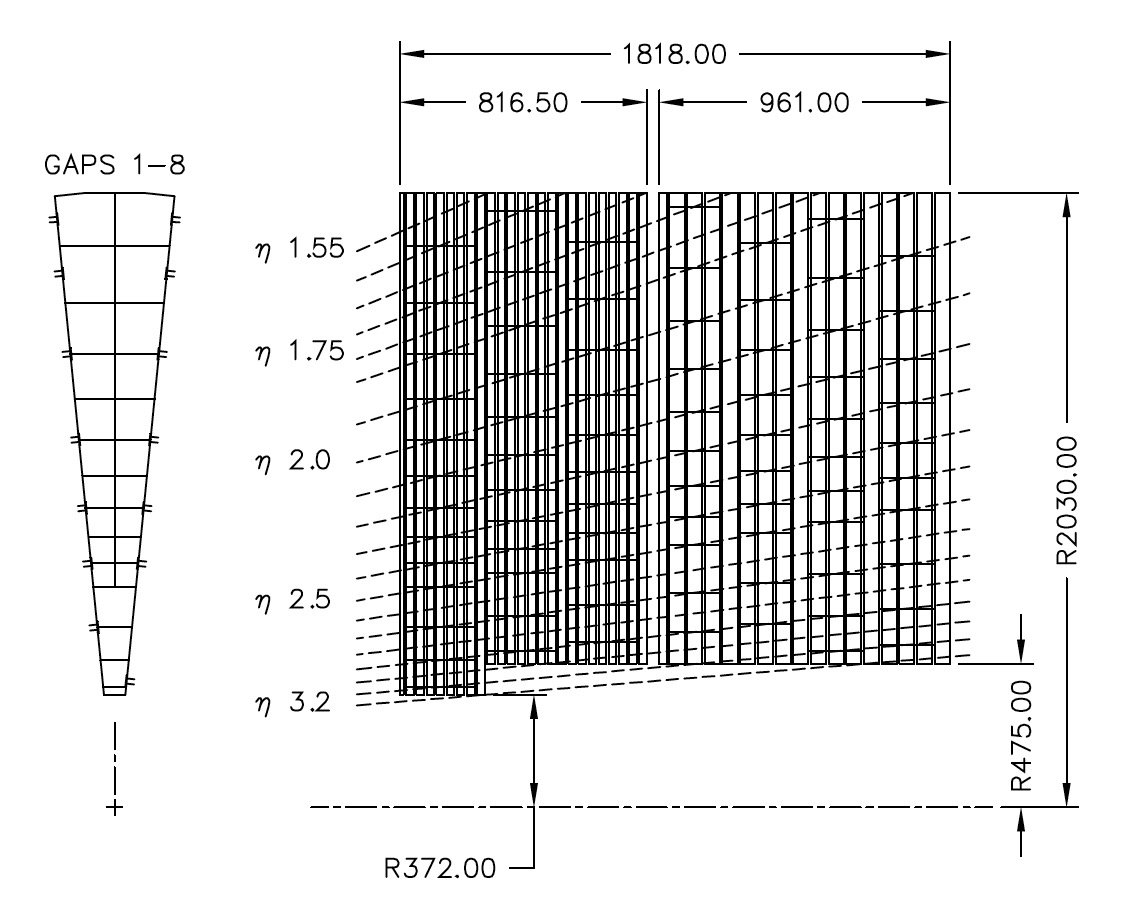
\includegraphics[width=0.75\textwidth]{figuresEXP/ATLASCA4.jpg}
  \end{center}
  \caption{
ATLAS端盖强子量能器沿$R$-$\phi$平面(左图)和$R$-$z$平面(右图)的截面图,单位是mm。
  }
    \label{fig:ATLASCA4}
\end{figure}

前端量能器是一个组合型量能器,
能同时测量因电磁簇射和强子簇射而沉积的能量。
它距对撞点仅4.7m,分为左右两部分,覆盖了$3.1<|\eta|<4.9$的范围,
能量分辨率为:
\begin{equation} 
\label{eq:EMsigma3}
\frac{\sigma(E)}{E}=\frac{100\%}{\sqrt{E}}\oplus 10\%
\end{equation}
由于其所处位置的粒子通量较大,因此采用了密封式设计,
这样能使粒子在各个量能器模块间的隙缝中的能量损失降到最低,
还能限制簇射粒子到达$\mu$子谱仪。
如图~\ref{fig:ATLASCA5}~所示,每个部分又可以分为三个紧密相连的模块,
依次是一个电磁量能模块(FCal1)和两个强子量能模块(FCal2, FCal3)。
三个模块都用液氩作为活性材料,
为了优化分辨率和快速散热,
电磁量能模块用铜作为吸收材料,
强子量能模块用钨作为吸收材料,
钨能有效的防止来自强子簇射的粒子从侧面扩散出去。
%来防止来自强子簇射的粒子横向扩散出去并保证其封闭性。

\begin{figure}
  \begin{center}
    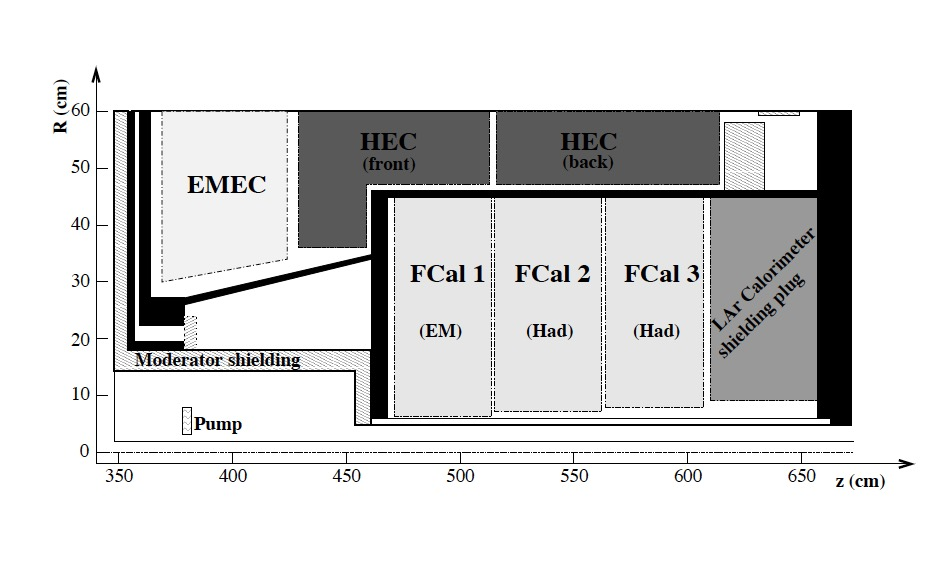
\includegraphics[width=0.75\textwidth]{figuresEXP/ATLASCA5.jpg}
  \end{center}
  \caption{
ATLAS前端量能器的示意图。
其中包含三个模块,依次是一个电磁量能模块(FCal1)和两个强子量能模块(FCal2, FCal3)。
  }
    \label{fig:ATLASCA5}
\end{figure}





\subsection{$\mu$子谱仪}
\label{sec:ATLASMSP}

$\mu$子谱仪(The Muon Spectrometer, MS)~\cite{ATLASMUSPEC}位于ATLAS探测器的最外部,
由精密室(The precision-measurement tracking chambers)和触发室(The trigger chambers)两大部分组成,
%从径向半径5m处延伸到接近10m的位置,
用于重建$\mu$子的径迹和动量。
由于$\mu$子与量能器材料的相互作用截面极低,
它们在穿过量能器时仅损失很小的一部分能量,
在离开量能器之后被$\mu$子谱仪探测到。
精密室用于在$|\eta|<2.7$的范围内重建离开量能器之后的$\mu$子动量,
%通过
结合内部探测器中的信息,可以重建出完整的$\mu$子动量,
%可以重建出来自对撞点的$\mu$子动量信息,
触发室能在$|\eta|<2.4$的范围快速触发$\mu$子的径迹。

精密室由可监控漂移腔室(The Monitored Drift Tubes, MDT)~\cite{ATLASMDT}和阴极剥离腔室(The Cathode Strip Chambers, CSC)两部分组成。
可监控漂移腔室用于测量桶部覆盖的$z$坐标和端盖覆盖的$|\eta|<2.7$范围内的$\mu$子动量,
它的基本组件元是压力漂移管,
每个压力漂移管直径为30mm,管内充满了
%处于3bar恒压的
$Ar/CO_2$混合气体,
管壁作为阴极,管内中心有一根直径为50$\mu m$的钨铼合金丝作为阳极。
如图~\ref{fig:ATLASMS1}~所示,
$\mu$子穿过压力漂移管时会使管内混合气体电离,
产生的电子和正离子分别向合金丝和阴极漂移,从而触发电信号。
精密室总共包含1150个可监控漂移腔室,可监控漂移腔室的平均分辨率为35$\mu m$($z$),每个腔室由3到8层压力漂移管组成。
高横动量$\mu$子的动量测量精度取决于弧矢的分辨率,即$R$-$z$平面上$\mu$子圆弧径迹相对于弦的偏差,
对于横动量为1TeV的子,对应的弧矢大约为500$\mu m$,
而可监控漂移腔室对横动量在10GeV和1TeV之间的$\mu$子的测量精度$\sigma_{p_{T}}/p_{T}$在$2\%$到$10\%$之间。

\begin{figure}
  \begin{center}
    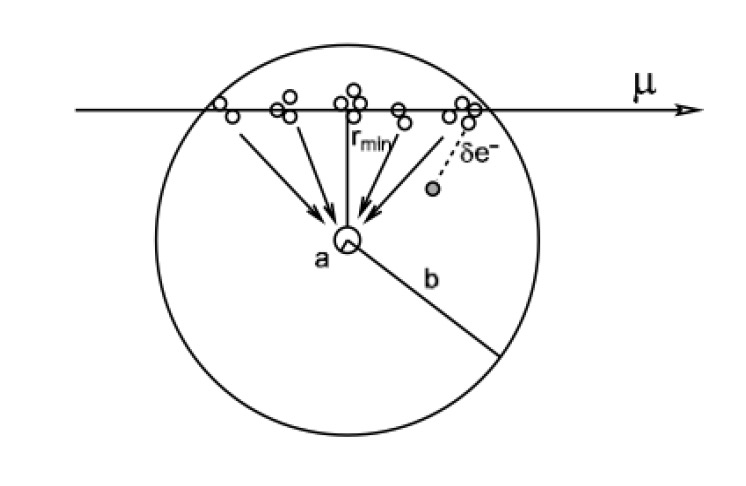
\includegraphics[width=0.5\textwidth]{figuresEXP/ATLASMS1.jpg}
  \end{center}
  \caption{
  $\mu$子穿过$\mu$子谱仪的可监控漂移腔室中压力漂移管的示意图。
漂移管中混合气体被$\mu$子电离之后,产生的电子会向阳极漂移。
  }
    \label{fig:ATLASMS1}
\end{figure}

阴极剥离腔室是多线程腔室,如图~\ref{fig:ATLASMS2}~所示,
它是由沿径向的
%带正电的
阳极线阵和包围它们的
%带负电的
铜质阴极组成,
其间充满了$Ar$、$CO_2$和$CF_4$混合气体,
用来测量前向区域$2<|\eta|<2.7$范围内的$\mu$子动量。
精密室总共包含32个阴极剥离腔室,
腔室的分辨率为$40\mu m\times5mm$($R\times\phi$)。

\begin{figure}
  \begin{center}
    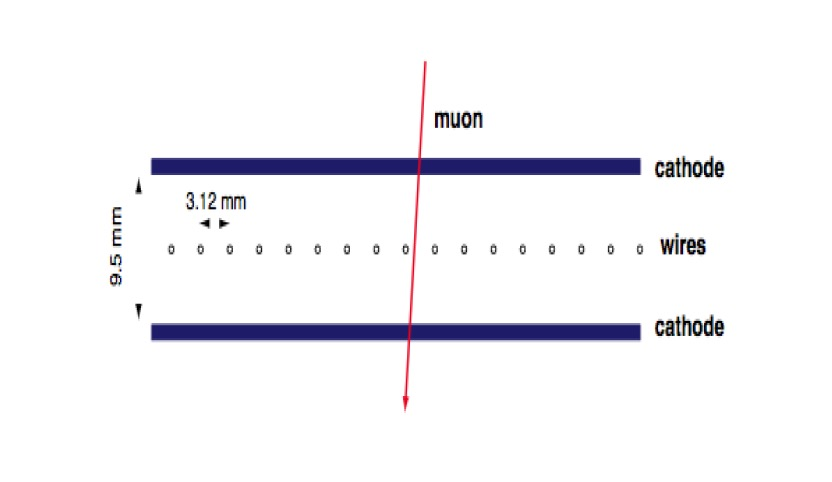
\includegraphics[width=0.6\textwidth]{figuresEXP/ATLASMS2.jpg}
  \end{center}
  \caption{
$\mu$子谱仪中的阴极剥离腔室的截面图。
  }
    \label{fig:ATLASMS2}
\end{figure}

$\mu$子谱仪非常重要的一个
%设计标准
性能指标是其触发$\mu$子径迹的能力,
%以区分$\mu$子的多样性和近似的能量范围。
%因此
为了弥补精密室的功能,触发室可以用于$\mu$子触发,
它能在$\mu$子通过之后的几十纳秒内传递该$\mu$子的径迹信息。
触发室可以分为电阻板腔室(The Resistive Plate Chambers, RPC)~\cite{ATLASRPC}和薄隙腔室(The Thin Gap Chambers, TGC)~\cite{ATLASTGC},
其中电阻板腔室由两个高电阻率的平行塑料板组成,
一个带正电的阳极和一个带负电的阴极,
两极板之间中间充满了$C_2H_2F_4$、$C_4H_{10}$和$SF_6$混合气体。
如图~\ref{fig:ATLASMS3}~所示,每个极板有两个正交的读出信道:
$\eta$信道平行于可监控漂移腔室的阳极合金丝;
$\phi$信道垂直于可监控漂移腔室的阳极合金丝。
电阻板腔室覆盖了$|\eta|<1.05$的范围,
其空间分辨率为$10mm\times10mm$($z\times\phi$),时间分辨率达到了1.5ns。

\begin{figure}
  \begin{center}
    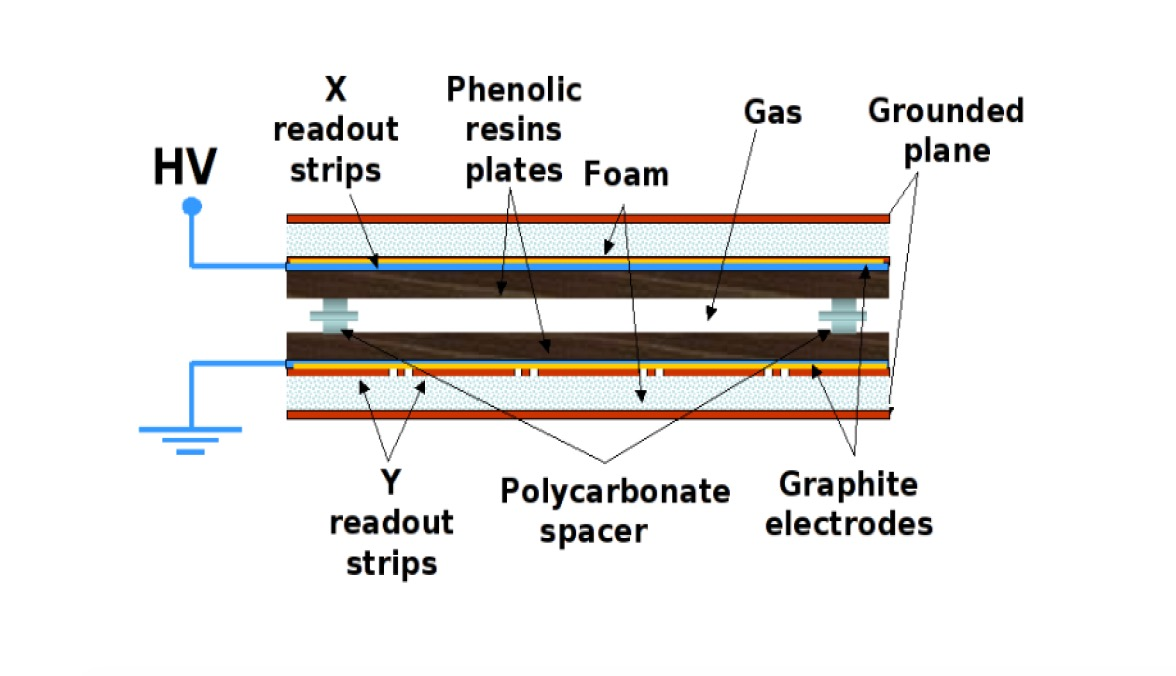
\includegraphics[width=0.6\textwidth]{figuresEXP/ATLASMS3.jpg}
  \end{center}
  \caption{
  $\mu$子谱仪中的电阻板腔室的结构示意图。
%电阻板腔室结构简图。
  }
    \label{fig:ATLASMS3}
\end{figure}

%薄隙腔室由两块作为阴极的接地电阻板和夹在其中的带有正高压的保持一定间隔的导线阵列组成,
薄隙腔室由两块电阻板和位于中间的一排导线阵列组成,
如图~\ref{fig:ATLASMS4}~所示,
其中两块电阻板接地作为阴极,相距2.8mm,
其间充满了$CO_2$/n-$C_5H_{12}$混合气体,
导线阵列中导线间隔为1.8mm,带有正高压,
作为阳极,它平行于可监控漂移腔室的阳极合金丝,并接有读出信道,能用于信号触发。
%覆盖了$1.05<|\eta|<2.4$的范围。
%阴极电阻板板之间是$CO_2$/n-$C_5H_{12}$混合气体。
%阴极导线平行于可监控漂移腔室的阳极合金丝,并接有读出信道,能用于信号触发。
薄隙腔室覆盖了$1.05<|\eta|<2.4$的范围,
%同样
也具有非常好的时间和空间分辨率,其空间分辨率主要由阴极导线的数量决定。


\begin{figure}
  \begin{center}
    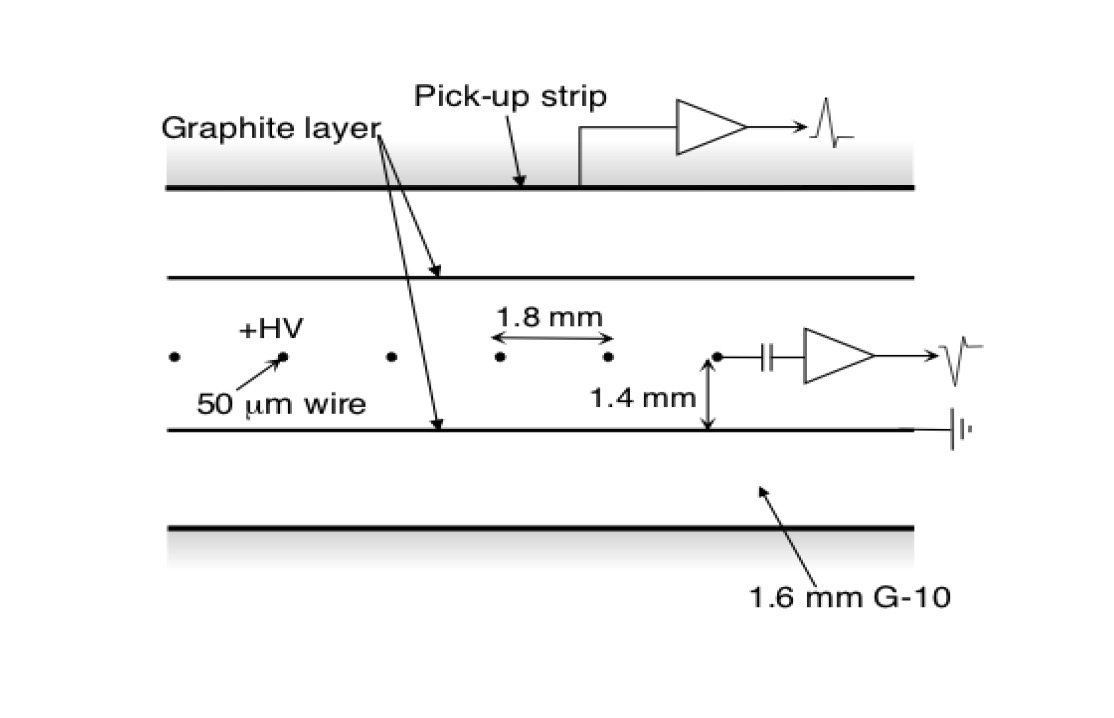
\includegraphics[width=0.6\textwidth]{figuresEXP/ATLASMS4.jpg}
  \end{center}
  \caption{
  $\mu$子谱仪中的薄隙腔室的结构示意图。
%薄隙腔室的结构简图。
  }
    \label{fig:ATLASMS4}
\end{figure}

%图~\ref{fig:ATLASMS5}展示了$\mu$子谱仪在$x$-$y$平面和$z$-$y$平面的截面图,其内部结构和前述各个子探测器都有标注。
表~\ref{tab:ATLASTab2}~总结了$\mu$子谱仪的各个子结构的主要参数。

%\begin{figure}
  %\begin{center}
    %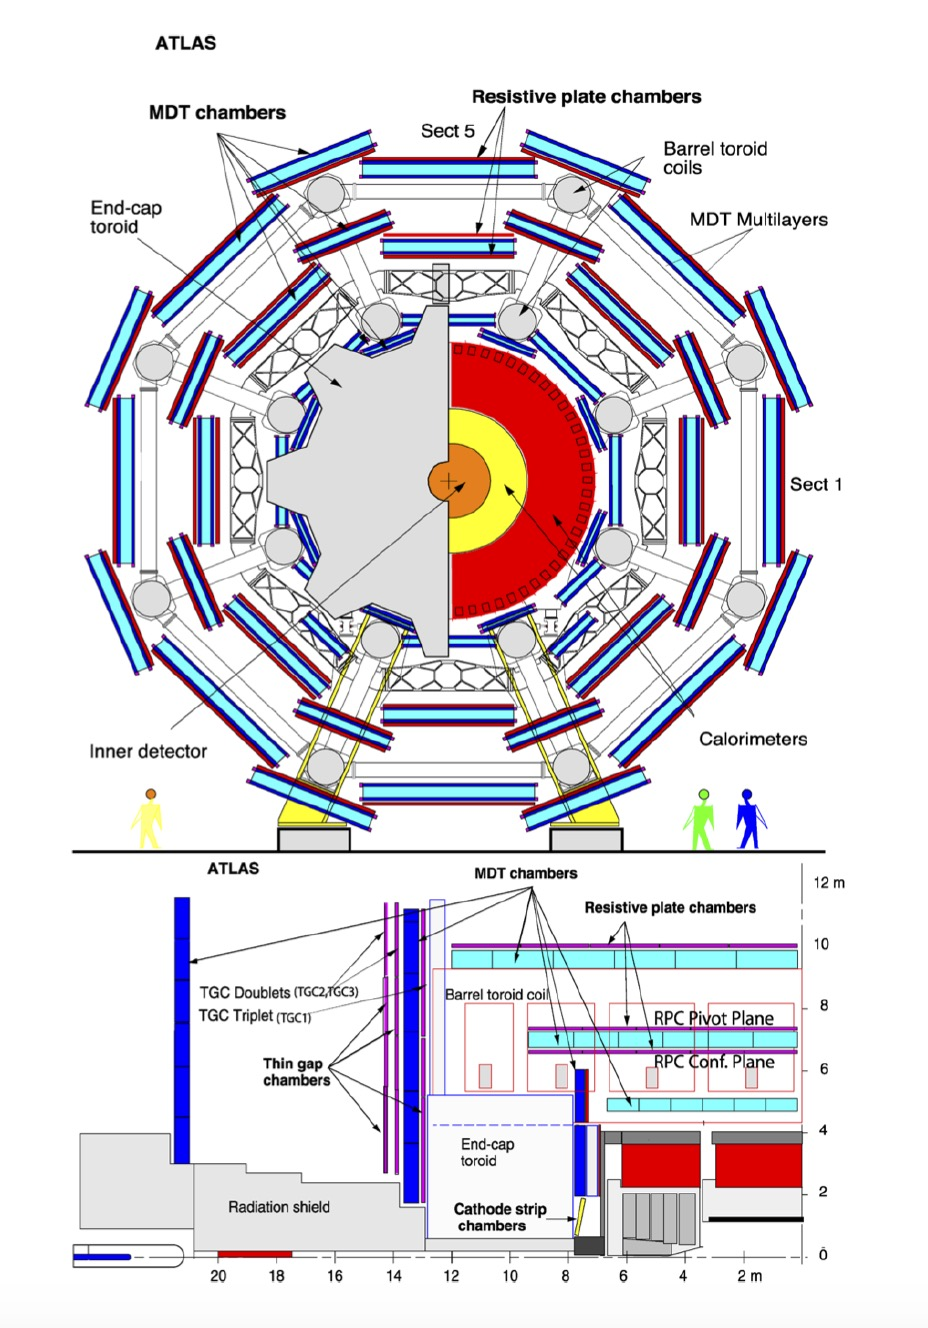
\includegraphics[width=0.75\textwidth]{figuresEXP/ATLASMS5.jpg}
  %\end{center}
  %\caption{
%$\mu$子谱仪在$x$-$y$平面(上)和$z$-$y$平面(下)的截面图。
 % }
   % \label{fig:ATLASMS5}
%\end{figure}

\begin{table}[htbp]
      \caption{
%$\mu$子谱仪的四个子探测器的参数。  
$\mu$子谱仪的各个子结构的主要参数。    
      }
      \label{tab:ATLASTab2}
      \centering
      \begin{adjustbox}{width=\columnwidth,center}
      \begin{tabular}{|c|c|c|c|c|c|c|c|c|}
        \hline
         Type & Function  &   \multicolumn{3}{c|}{Chamber resolution in}   &   \multicolumn{2}{c}{Measurements/track}   &   \multicolumn{2}{|c|}{Number of}  \\
         \hline
         &   &  $z/R$ & $\phi$  & time  & barrel  & end-cap  &  chambers &   channels \\
         \hline
         MDT& tracking  & 35$\mu m(z)$ & -  &  - & 20  &  20 & 1150  &  354k \\
         \hline
         CSC& tracking  & 40$\mu m(R)$  &  5mm &  7ns &  - &  4 & 32  & 30.7k  \\
         \hline
         RPC& trigger  &  10$mm(z)$ & 10mm  & 1.5ns  &  6 & -  & 606  &  373k \\
         \hline
         TGC& trigger  & 2-6$mm(R)$  & 3-7mm  & 4ns  &  - & 9  & 3588  &  318k \\
         \hline
      \end{tabular}
      \end{adjustbox}
\end{table}

\subsection{触发和数据采集系统}
\label{sec:ATLASTDAS}

触发和数据采集系统~\cite{ATLASTDAQ}是ATLAS探测器的重要组成部分,
%它负责决定是否将庞大的数据中给定的碰撞事例保存下来作为一个值得研究的物理过程用于后续的离线分析。
它负责有选择性的将庞大的数据中一小部分保存下来用于后续的离线分析。
$Run\_2$计划相对于$Run\_1$计划有着更高的亮度和对撞能量,
因此$Run\_2$计划之前,
必须对ATLAS的触发和数据采集系统进行升级,
%对ATLAS探测器的触发和数据采集系统进行了升级,
升级之后的系统需要将
质子束碰撞频率(The bunch crossing rate)高达40MHz的数据减小到1kHz并记录下来,
这也是数据处理所能达到的最高频率。

如图~\ref{fig:ATLASTS1}~所示,
%$Run\_2$计划整个
升级之后,
ATLAS的触发系统~\cite{ATLASRTS}由基于硬件的一级触发器(First Level Trigger)和
基于软件的高级触发器(High Level Trigger)组成。
一级触发器有量能器一级触发和$\mu$子一级触发两种类型,
它可以访问粗粒度量能器和$\mu$子谱仪中的原始数据,
并基于粒子的多样性和$\mu$子横动量等信息作出决策,
进行事例的初步筛选。
一级触发器能将40MHz的质子束碰撞频率降低到100kHz,
%总延迟为2.5$\mu s$,
筛选出来的信息随后会被送到高级触发器,
进一步将质子束碰撞频率降低到1kHz。
高级触发器用于进一步的离线筛选和对象重建,为后续的物理分析做准备。

\begin{figure}
  \begin{center}
    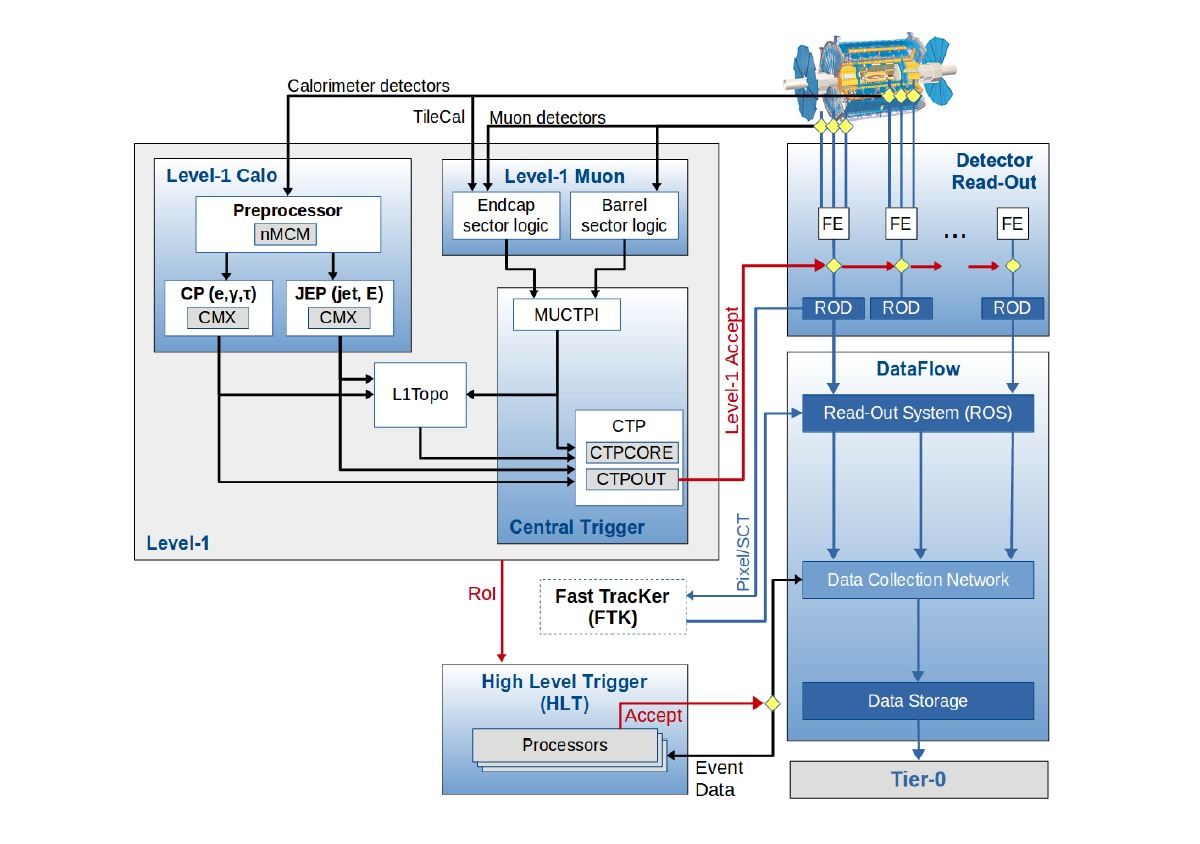
\includegraphics[width=0.75\textwidth]{figuresEXP/ATLASTS1.jpg}
  \end{center}
  \caption{
ATLAS的触发和数据采集系统的结构示意图。
  }
    \label{fig:ATLASTS1}
\end{figure}

\subsection{亮度探测器系统}
\label{sec:ATLASLD}

ATLAS的亮度探测器系统~\cite{ATLASLUMID}用来测量束流亮度,并通过比较几个不同的亮度探测器的测量结果来确定亮度的误差。
如图~\ref{fig:ATLASLD1}~所示~\cite{LDIm},整个系统位于ATLAS探测器的前端,
由切伦科夫亮度探测器(The Luminosity measurement using Cerenkov Integrating Detector, LUCID)、
零能探测器(The Zero-Degree Calorimeter, ZDC)和绝对亮度探测器(The Absolute Luminosity For ATLAS, ALFA)三个子探测器依次排列组成。
切伦科夫探测器离对撞点最近,仅$\pm 17m$,覆盖了$5.6<\eta<6$的范围,
它可以通过在接收范围内计数每次对撞中产生的带电粒子数来计算非弹性质子-质子对撞的平均次数,
从而监控前端的非弹性质子-质子散射率,它既可以测量积分亮度,也可以在线监控瞬时亮度。
零能探测器位于离对撞点$\pm 140m$、$8.3<\eta$的位置,
它主要通过探测对撞过程中产生的正向中子来测量相对亮度,
它可以测量质子-质子对撞的亮度,也可以测量重离子对撞的亮度,
绝对亮度探测器距离对撞点$\pm 240m$,覆盖了$10.6<\eta<13.5$的范围,
它是由闪烁体纤维组成,通过在小角度上探测质子-质子散射来确定绝对亮度和总的质子-质子散射截面。

\begin{figure}
  \begin{center}
    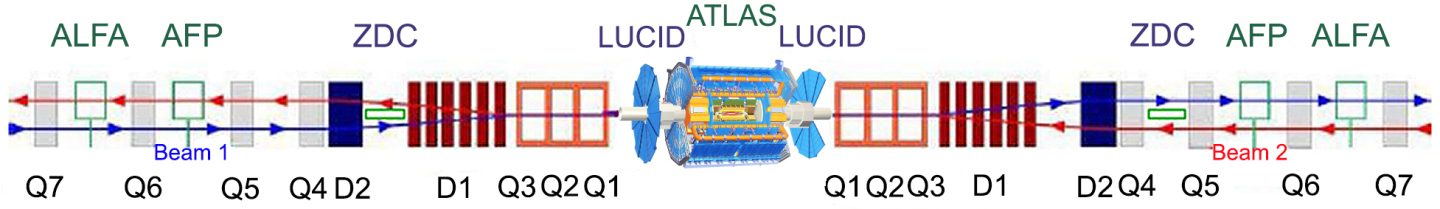
\includegraphics[width=0.98\textwidth]{figuresEXP/ATLASLD1.jpg}
  \end{center}
  \caption{
ATLAS的亮度探测器系统。
  }
    \label{fig:ATLASLD1}
\end{figure}


\section{MC模拟}
\label{sec:Simulation}

%为了使用理论模型对实验结果作出准确的预测,
为了对理论模型进行有效的验证,
需要对碰撞事例的产生及粒子与探测器的相互作用过程进行精确的Monte Carlo(MC)模拟,
MC模拟是高能物理中非常关键的一步,
ATLAS合作组有一套完善的模拟系统~\cite{ATLASMC},
%可以
用于实验分析的诸多方面,
包括与模型对应的实验可观测量的预测、分析优化和系统误差的确定等。
%包括标准模型的预测、校准、分析优化和系统误差的确定等,
%本章将做简要介绍。

\subsection{硬散射和部分子簇射}
\label{sec:MCHS}

%MC模拟中关键的一环是对被模拟的硬散射过程的截面的计算。
MC模拟中关键的一环是
%对被模拟的
硬散射(Hard scattering)过程的截面计算,
而截面计算主要依赖于QCD因式分解定理~\cite{MC1}。
结合部分子分布函数(Parton Distribution Functions, PDFs)~\cite{MC2},
该定理可以将低横动量部分子相互作用与代表硬散射过程的高横动量部分子相互作用过程分离,
%部分子硬散射过程分离。
其中
%不参与硬散射过程的
低横动量部分子相互作用产生的事例被称为潜在事例(The underlying event)~\cite{MC3},
对于特定的过程,
%部分子
硬散射过程的截面与矩阵元模的平方成正比,
对于这部分,可以使用微扰论进行计算,
%对相互作用的耦合常数进行展开,
%从而
用展开后的高阶有限项近似成硬散射的截面,
并且展开后的每一项都可以用费曼规则~\cite{FEYNR}进行计算。

%\subsection{部分子分布函数和部分子簇射}
%\label{sec:MCPDF}
其中部分子分布函数是一个经验式函数,
在不同的实验合作组有不同的结果,
它给出了部分子携带入射质子纵向动量的分数x的概率,
并且依赖于硬散射过程中的动量传递,
利用它可以实现质子的动量和参与硬散射过程的部分子动量之间的转换~\cite{MC1}。
部分子发生硬散射后,都会辐射其他部分子,这个过程称为部分子簇射~\cite{MC6},
它和硬散射过程
%一起
都可以由部分子簇射模拟器\textsc{Pythia}~\cite{MC5}来模拟。


\subsection{强子化}
\label{sec:MCHARD}

如第~\ref{cha:Theory}~章所述,由于QCD中色禁闭的性质,
夸克或胶子在产生之后会通过强子化形成不带色荷的强子束缚态。
%并且QCD中
由于渐近自由的性质,强子化过程不能用微扰论进行计算,
%即无法从第一性原理来解释这个过程,从而需要建模来描述强子化。
需要建模对其进行描述,
%强子化建模的主流模型有两个:
主流的强子化模型有两种:
Lund弦模型(the Lund string model)~\cite{Hadonization}和簇模型(the cluster model)~\cite{MC4}。
在Lund弦模型中,如图~\ref{fig:MC1}~所示,夸克通过随着夸克分离而拉伸的弦连接在一起,
这些弦可以被拉断,同时会在新弦的末端产生一个夸克-反夸克对,
过程一直持续到能量不足以拉断夸克之间的弦,
并且所有的夸克都通过弦的断裂形成强子为止。

%这种模型的强子化过程可以由部分子簇射模拟器\textsc{Pythia}~\cite{MC5}来模拟完成,
Lund弦模型可以由\textsc{Pythia}~\cite{MC5}来模拟,
它可以同时用于事例产生和矩阵元产生。
%接下来便是
对于矩阵元的计算和
%模拟
不稳定强子的衰变过程,
分别可以由\textsc{MadGraph5}~\cite{Alwall:2014hca}和\textsc{Evtgen}~\cite{Lange:2001uf}来模拟。
%其他不稳定粒子的衰变可以在\textsc{Pythia}内完成。

\begin{figure}
  \begin{center}
    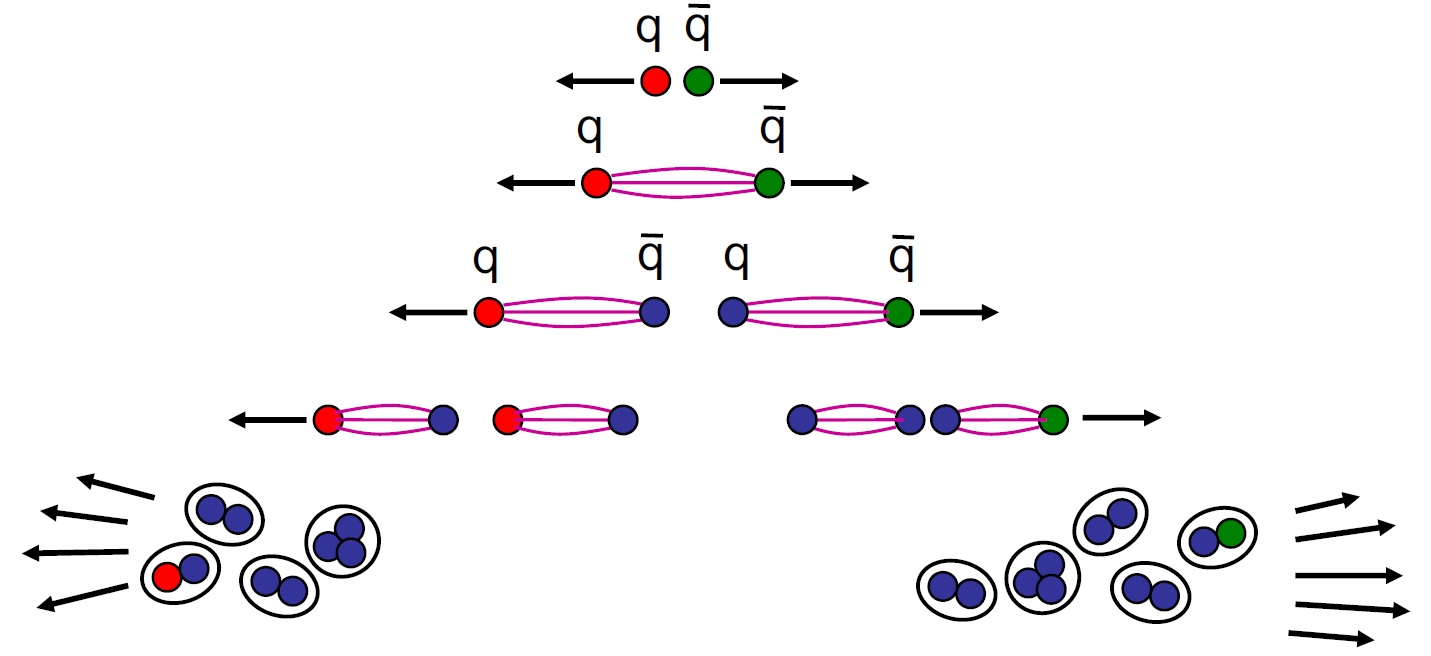
\includegraphics[width=0.9\textwidth]{figuresEXP/MC1.jpg}
  \end{center}
  \caption{
Lund弦模型中的强子化过程。
  }
    \label{fig:MC1}
\end{figure}


\subsection{探测器模拟}
\label{sec:MCDET}

%所模拟的质子-质子对撞产生的粒子
MC模拟的质子-质子对撞事例产生的长寿命粒子
与探测器材料的相互作用和最终的电子学读出是用\textsc{Geant4}~\cite{MC7}模拟的,
它能准确模拟ATLAS探测器中的各种探测器材料的性质和其几何形状,并
%精确
完整的重现粒子与探测器材料的相互作用行为。
传统的模拟过程以非常精确的方式模拟探测器的响应,对可能影响粒子的任何微小结构都会进行建模,称为全模拟(Full simulation),
这种方法非常耗时,也非常耗费资源。
因此,为了节省时间和资源,同时满足不同粒子在
%不同研究
特定物理分析中的重要程度以及过程对不同子探测器的精度要求,
构建了一种快模拟(Fast simulation)~\cite{MC8}的方法,
%它能通过参数化对探测器材料和有源探测器元件的响应进行建模,
它能将粒子对探测器材料和
%有源
探测器元件的响应参数化,
这种方法的明显缺点是降低了精度,但对于某些研究过程
%的粒子响应
是可以接受的。


\section{物理对象的重建}
\label{sec:Reconstruction}

数据采集完成之后,
接下来的任务便是重建用于实际物理分析的
%基本
物理对象。
质子-质子对撞
%硬散射事例
产生的粒子中仅有一小部分寿命足够长到能被ATLAS探测到,
大部分粒子产生之后都会
%通过
衰变或级联衰变成更轻、更稳定的粒子。
%进而被被ATLAS探测到。
在已知的所有基本粒子和复合粒子中~\cite{PDG},只有十四种粒子的平均自由程大于500$\mu m$,
%从而
能与探测器材料相互作用并被探测到,它们分别是$\mu$子($\mu^+$, $\mu^-$)、电子($e^+$, $e^-$)、光子($\gamma$)、
$\pi$介子($\pi^+$, $\pi^-$)、K介子($K^+$, $K^-$, $K_L^0$)、质子($p^+$, $p^-$)和中子($n^+$, $n^-$)。
%由于强相互作用具有色禁闭的性质,
在第~\ref{sec:MCHARD}小节中提到,夸克或胶子产生之后会经过强子化过程
%~\cite{Hadonization}
形成色中性的强子束缚态,
%并在探测器中产生高度准直的强子簇射,被称为喷注或jet~\cite{JETS},
并在探测器中产生高度准直的圆锥形粒子簇射,称为喷注或jet~\cite{JETS},
其中包含b强子的jet具有独特的内部性质,记为b-jet,
%jet的重建是
上述十四种长寿命粒子中的九种强子便是夸克或胶子在强子化过程中产生的。
由于中微子仅参与弱相互作用,而且相互作用截面极小,因此不能被ATLAS探测到,
它的存在是通过在碰撞前后事例整体的横动量守恒来推断的。
%即丢失横动量的重建。
$\tau$子的寿命为$2.9×10^{−13}s$,在进入内部探测器之前就会衰变,可以通过它的衰变产物来进行重建。
接下来将会简要介绍这些物理对象的重建过程。


\subsection{径迹和顶点的重建}
\label{sec:TRACKS}

%径迹可以用来识别碰撞产生的粒子和碰撞顶点,
径迹可以用于识别带电粒子的类型和重建碰撞顶点,
%它是通过使用一系列算法从粒子在内部探测器中留下的信息中重建的~\cite{TRACK1}。
它是通过一系列算法从内部探测器中重建出来的~\cite{TRACK1}。
%首先,将带电粒子在PD和SCT探测器部分结构中留下的电信号转化成三维的空间位置信息。
首先,将带电粒子在PD和SCT探测器中留下的电信号转化成三维的空间位置信息,
如图~\ref{fig:ATLASORT1}~所示,由单个带电粒子形成的点簇称为单粒子点簇,
由多个带电粒子形成的点簇称为合并点簇。
%合并点簇的识别和分离是通过一个基于机器学习的集群算法实现的~\cite{NNCLUSTER}。
%然后通过三维空间位置信息中的每三个点构建径迹种子池,
%其中它们的动量和碰撞参数必须满足一定的筛选条件,
然后在空间位置信息中构建径迹种子池,种子池中径迹由三个位置点组成,
其动量和碰撞参数满足一定条件,而且要求种子池中还包含与其兼容的第四个位置点,
其中合并点簇的识别和分离是通过一个基于机器学习的集群算法实现的~\cite{NNCLUSTER}。
%而且种子池中每条径迹必须要有与之兼容的第四个点。
随后通过结合
%与种子池中径迹兼容的
来自内部探测器中其他子探测器的空间位置信息,
利用\textsc{KalmanFilter}
%算法
~\cite{KALMAN}从种子池中构建候选径迹,
%随后通过结合与种子池中径迹兼容的来自PD和SCT探测器其他结构中的空间位置信息,
%利用\textsc{KalmanFilter}~\cite{KALMAN}从径迹种子池中构建候选径迹。
候选径迹构建完成之后,
会引入一个解决歧义的算法~\cite{TRACK1}来修正部分候选径迹的所属点有重叠或者分配错误的问题。
最后,便是对候选径迹中的点进行高分辨率的拟合。

\begin{figure}
  \begin{center}
    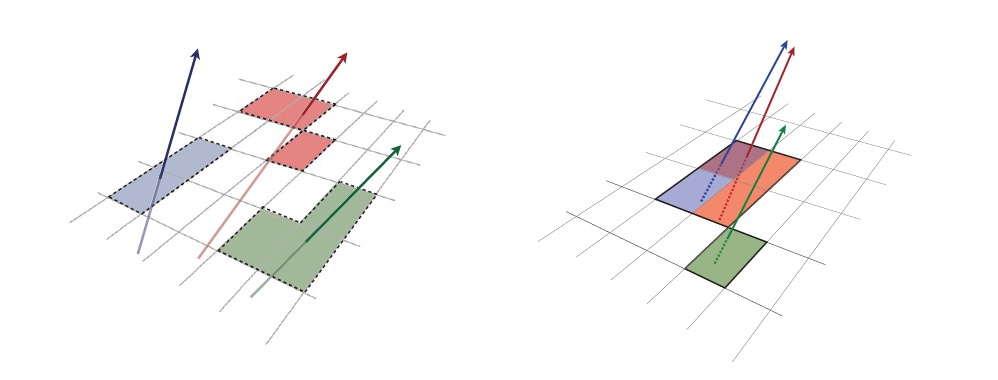
\includegraphics[width=0.9\textwidth]{figuresEXP/ATLASORT1.jpg}
  \end{center}
  \caption{
像素传感器上的单粒子点簇(左)和合并点簇(右)示意图。
  }
    \label{fig:ATLASORT1}
\end{figure}


%质子-质子硬散射的起点也就是主顶点的重建~\cite{VERTEX1,VERTEX2}对于实际的物理分析来说至关重要,
硬散射的顶点也就是主顶点和次级顶点的重建~\cite{VERTEX1,VERTEX2}对于实际的物理分析来说至关重要,
它们不仅有助于后续物理对象的重建,还能有效的压低堆积事例。%~\cite{PileUp}。
%主
顶点是利用内部探测器中的径迹重建出来的,
%在内部探测器中重建出来的径迹重建出来的,
首先按一定条件从候选径迹中筛选出一部分用于顶点重建,
并为这些
%满足条件的
径迹分配一个合适的候选顶点,
然后通过对候选顶点和径迹进行一个迭代拟合过程来寻找最优的顶点位置,
在每次迭代中,会减小兼容性较低的径迹的权重,
%对兼容性较低的轨迹都会进行重新加权,
并重新计算顶点位置,
%随后与这个最优顶点不相关联的径迹会被挑出来用于确定下一个顶点,
最优顶点确定之后,与其不相关联的径迹会被筛选出来用于确定下一个顶点,
%重复之前的操作,
重复之前的操作,直到所有径迹都有与之关联的顶点或者在剩下的径迹中不能找到更多的顶点。

\subsection{量能器中拓扑集群的重建}
\label{sec:TOPTCLUS}


拓扑集群~\cite{TOPOCLUSTER}用于
%寻找
表征
量能器中来自硬散射
%过程
的高能粒子的能量沉积。
%同时
为了抑制来自于电子元件和堆积事例的噪声,
%这里
引入量能器单元的能量沉积信噪比$\varsigma_{cell}$用于后续拓扑集群的重建,
%它被
其定义为:
\begin{equation} 
\label{eq:TOPOSN1}
\varsigma_{cell}=\frac{E_{cell}}{\sigma_{noise,cell}}
\end{equation}
其中$E_{cell}$是量能器单元中沉积的能量,$\sigma_{noise,cell}$是量能器单元中噪声的期望值。
首先,选取满足$|\varsigma_{cell}|>4$的量能器单元作为
集群种子池,
%种子集群,
%然后与种子集群相邻的满足$|\varsigma_{cell}|>2$的量能器单元会被添加到临近的种子集群当中,构成新的种子集群,
对于这些集群,与其相邻并且满足$|\varsigma_{cell}|>2$的量能器单元将会被合并到对应集群当中,构成新的集群种子池,
%这个过程会被重复
重复这个过程,直到没有这样的邻近量能器单元。
%这样的重建过程是在三维尺度上完成的,
这个过程是在三维空间上完成的,
因此每个集群中的单元可能位于同一个量能器的同一模块,
也可能位于同一个量能器的不同模块或者不同的量能器。
最后,
对于新的种子池中集群,
与其相邻并且满足$|\varsigma_{cell}|>0$的量能器单元将会被合并到对应集群当中,
%所有与种子集群相邻的满足$|\varsigma_{cell}|>0$的量能器单元都会被合并到相对应的种子集群当中,
%到此,拓扑集群的重建便完成了。
%最后一
这个过程可能导致集群合并,
%如果一个集群内存在着明显的局部能量最大,
如果一个集群内存在多个明显的局部能量极大,
%那么
将会
%有另一种算法
对其进行拆分~\cite{TOPOCLUSTER},
到此,拓扑集群的重建便完成了。
%如图~\ref{fig:ATLASORT2}~所示,在$Run\_1$计划中用MC模拟的事例在前端量能器第一个模块中重建出来的拓扑集群示例图。

%\begin{figure}
  %\begin{center}
    %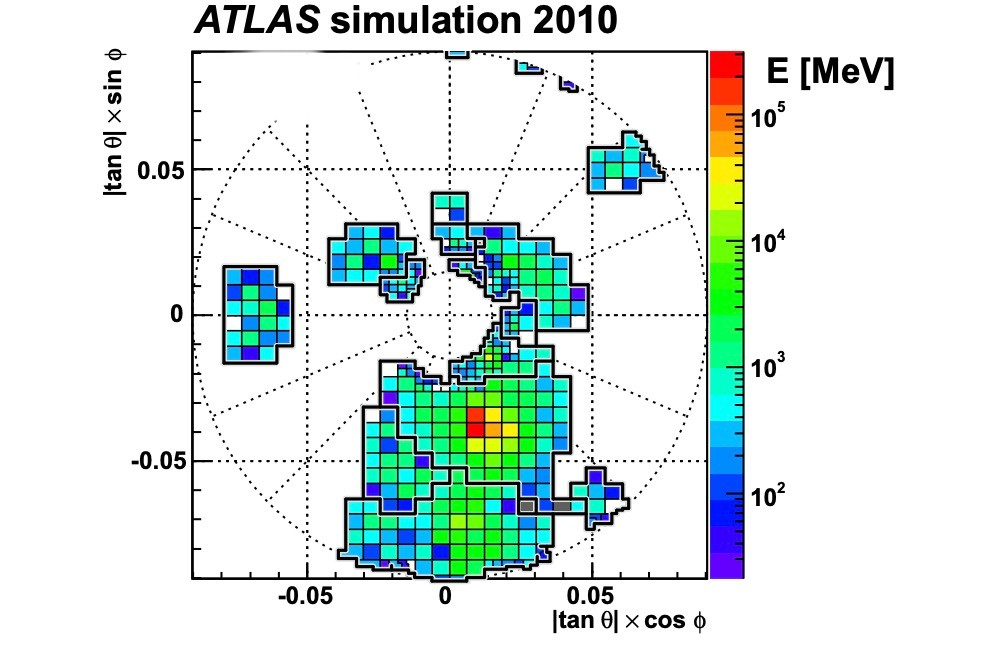
\includegraphics[width=0.75\textwidth]{figuresEXP/ATLASORT2.jpg}
  %\end{center}
  %\caption{
%用MC模拟的事例在前端量能器第一个模块中重建出来的拓扑集群示例图。
  %}
    %\label{fig:ATLASORT2}
%\end{figure}




\subsection{Jet的重建}
\label{sec:JET}

%夸克或胶子强子化之后以圆锥形粒子簇射的形式被探测器探测到,即jet。
前面提到,夸克或胶子是以jet的形式被探测到,
jet中带电粒子可以在内部探测器中留下径迹信息,
%随后连同jet中其他粒子一起沉积在电磁量能器和强子量能器中,
随后连同其他中性粒子一起沉积在量能器中,
因此,jet一般是从量能器的拓扑集群中重建出来的。
%如图~\ref{fig:ATLASJET1}~所示,
%首先,是在量能器系统中重建拓扑集群,这个过程在上一小节已有讨论。
%随后通过应用$anti$-$k_t$算法~\cite{ANTIKT}进行jet重建,
以拓扑集群为单元,jet重建是通过$anti$-$k_t$算法~\cite{ANTIKT}实现的,
该算法定义了一个
%拓扑集群
单元之间的距离度量$d_{ij}$和一个
单元
%拓扑集群
与束流之间的距离度量$d_{iB}$:
\begin{equation} 
\label{eq:TOPOSN}
\begin{split}
d_{ij}=&min\left( p_T^{2a}(i),p_T^{2a}(j) \right)\frac{\Delta R_{ij}^2}{R^2}
\\
d_{iB}=&p_T^{2a}(i)
 \end{split}
\end{equation}
其中$p_{T}(i)$和$p_{T}(j)$分别是单元i和单元j的横动量,
%如式~\ref{eq:DRdef}~中的定义,
$\Delta R_{ij}$是单元i和单元j在$\eta$-$\phi$平面的距离,
如式~\ref{eq:DRdef}~中的定义,
$a=-1$,$R$为距离参数。
然后,对于每个单元i,比较两种度量$d_{ij}$和$d_{iB}$的大小,
如果$d_{ij}$较小,则将单元i和单元j合并
成一个单元,
%到单个中间集群中,
如果$d_{iB}$较小,
那么将单元i认定为一个jet并从单元集中移除,
重复上述过程直到单元集为空集。
图~\ref{fig:ATLASJET1}~展示了利用$anti$-$k_t$算法重建出来的jet的示意图,
可以看到它们的形状都比较接近圆锥形。
%重复之前的操作直到这个集合中没有集群为止。
%利用量能器拓扑集群将jet重建完之后,
jet重建完成之后,
会通过一个“幻影”关联(Ghost association)的算法~\cite{Cacciari:2008gn}将内部探测器中带电粒子的径迹与jet进行匹配,
其中“幻影”是指径迹的横动量被设置成无穷小之后的四矢量,
基本只保留了径迹的方向信息,
随后再用anti-$k_t$算法将这个“幻影”和
jet中的拓扑集群重新会聚到这个jet中,
%构成jet的量能器拓扑集群重新会聚到这个jet中,
这样保证了重建出来的jet
与原来的jet是一致的,
%仍然是之前的jet,
如果此时“幻影”也是该jet的组成部分,
那么相应的径迹就和jet匹配上了。



\begin{figure}
 \begin{center}
    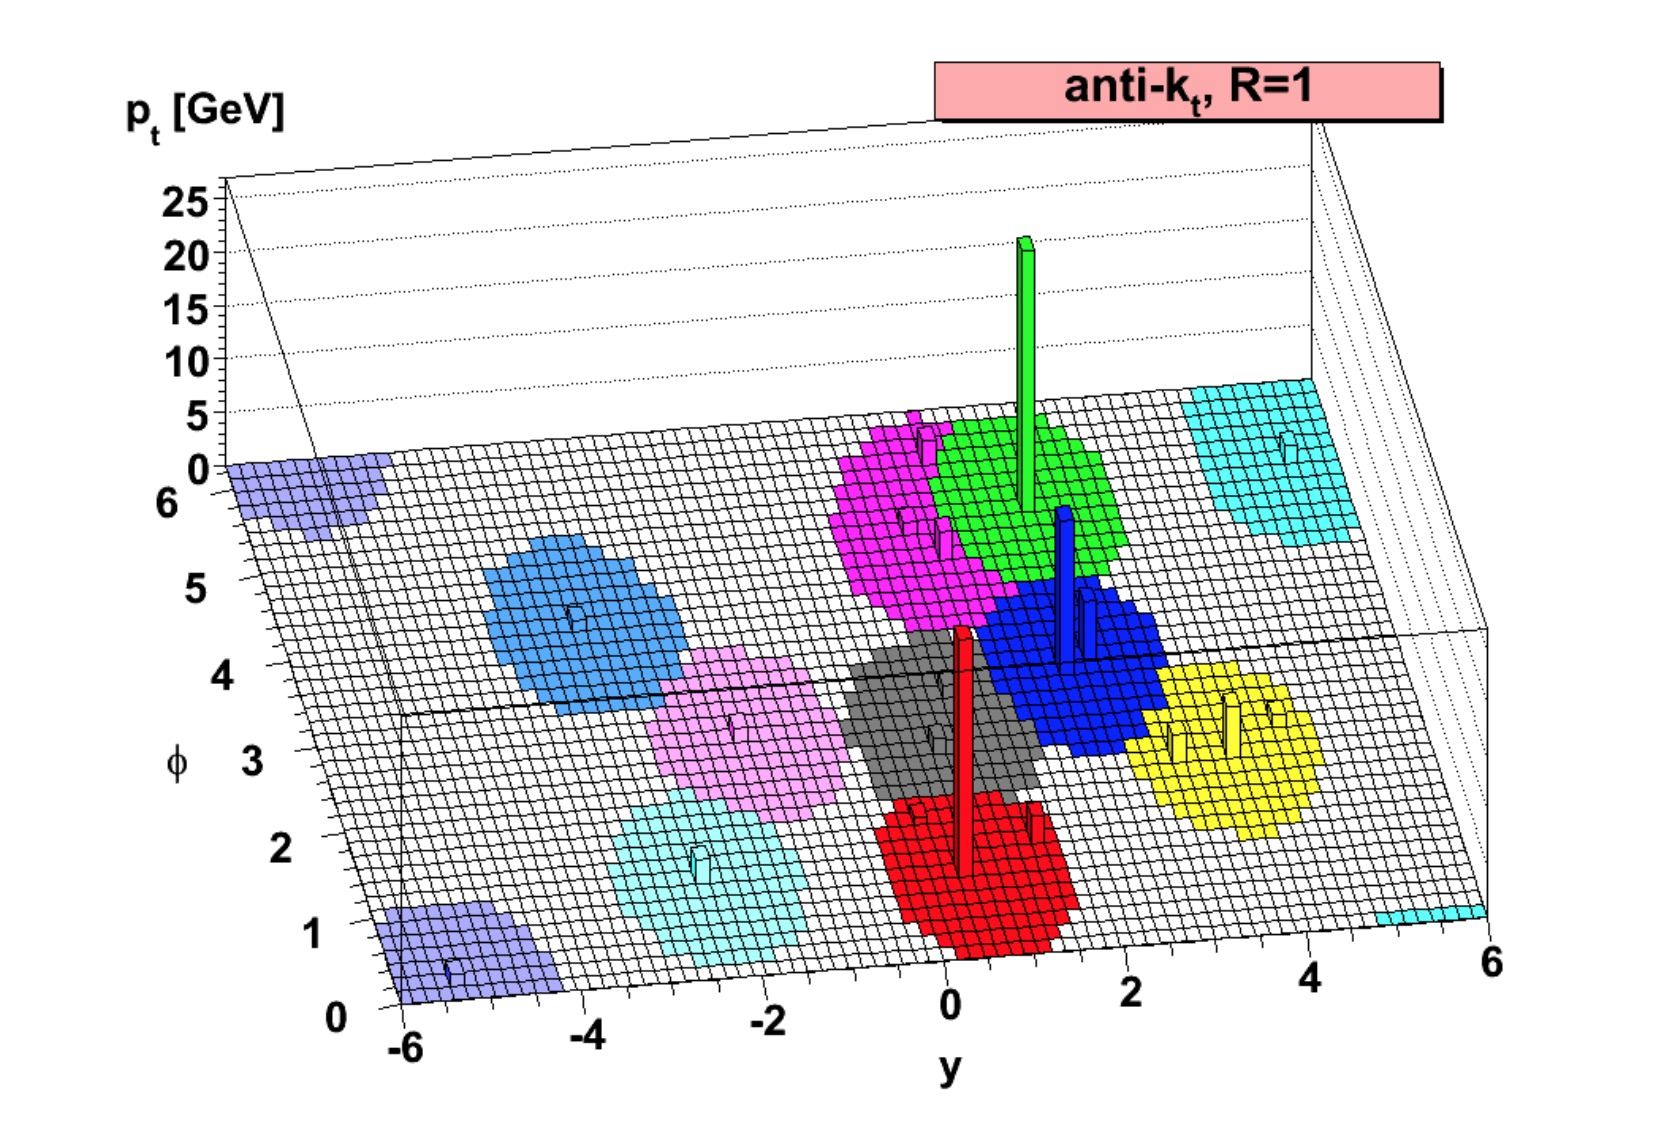
\includegraphics[width=0.75\textwidth]{figuresEXP/ATLASJET1.jpg}
  \end{center}
  \caption{
利用$anti$-$k_t$算法重建出来的jet的示意图,
%用$anti$-$k_t$算法进行jet重建的示例图。
%彩色区域表示重建出来的jet。
  }
    \label{fig:ATLASJET1}
\end{figure}


常用%的固定
的距离参数R有两个:
%使用R=0.4进行重建的jet代表
R=0.4所对应的是夸克或胶子
%强子化
在探测器中形成的jet,
记为SR-jet,
第~\ref{cha:Dijet}~章中的物理分析所使用的jet便是SR-jet;
%而使用$R=1$进行重建的jet代表
R=1所对应的是
强子型衰变的高横动量且大质量粒子
%比如说希格斯玻色子
在探测器中所形成的jet,
记为LR-jet,比如希格斯玻色子,
这也是第~\ref{cha:Xbb}~章中标定算法的开发所使用的一种jet。
%用$R=0.2$进行重建的jet代表包含在LR-jet中的小半径jet,记为FR-jet,章节~\ref{cha:Xbb}~中算法对比有用到这类jet。
%另外,合作组还引入了一种距离参数R可变的jet重建算法~\cite{VRJET1,VRJET2},记为VR-jet,
%在这个算法中,距离参数R是jet横动量$p_T$的函数:
%\begin{equation} 
%\label{eq:VR}
%R_{eff}(p_{T})=\frac{\rho}{p_T}
%\end{equation}
%其中新参数决定了有效的jet尺寸大小随着这个jet横动量动量减小的速度,
%除了之外,该算法还有两个附加的参数和分别对jet大小的上限和下限进行限制,
%这个限制可以防止jet在低横动量时变得太大或者在高横动量时收缩到探测器分辨率以下。
%这也是章节~\ref{cha:Xbb}~中新标定算法开发所使用的一种jet。
%FR-jet和VR-jet通常用于包含在LR-jet中的小半径jet,记为subjet的重建,
%如图~\ref{fig:ATLASJET2}~展示了利用FR-jet和VR-jet算法重建LR-jet中的subjet的简要示意图。


%\begin{figure}
  %\begin{center}
    %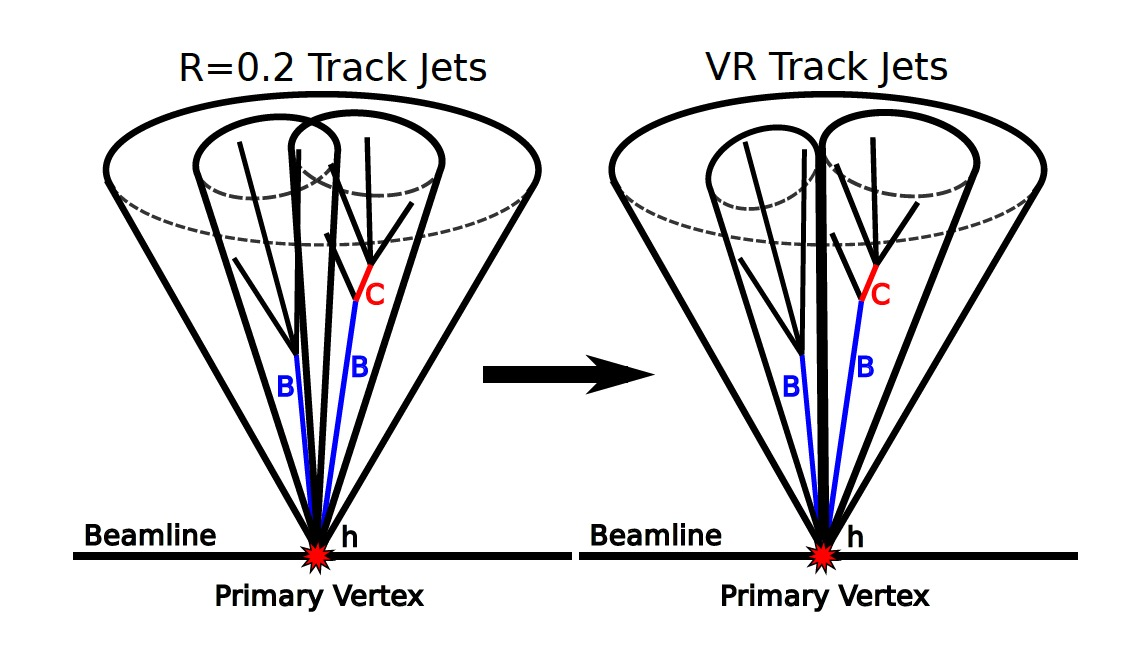
\includegraphics[width=0.9\textwidth]{figuresEXP/ATLASJET2.jpg}
  %\end{center}
  %\caption{
%使用固定半径$R=0.2$和可变半径重建LR-jet中的小半径jet的示意图。
  %}
    %\label{fig:ATLASJET2}
%\end{figure}


由于jet是一个由多粒子簇射形成的复杂对象,
%重建出来的非常复杂的对象,
因此需要通过参考MC模拟的真实对象和探测器的响应来校准它的能量。
%因此需要通过参考其他对象和模拟探测器响应来校准它的能量。
如图~\ref{fig:ATLASJET3}~所示,jet能量的校准主要分为以下几步~\cite{JES1}:
首先将jet的方向校准到
%指向
事例的主顶点,而不是探测器的中心,这样能显著提高$\eta$的分辨率~\cite{JES2};
然后基于jet在$\eta$-$\phi$平面
%的
覆盖的区域和该区域中jet的横动量密度,
从jet能量中移除来自
%相同和相邻质子束中
堆积事例的贡献~\cite{JES3};
%接着
%然后基于MC模拟的真实对象信息中主顶点的径迹数量和堆积事例率,修正jet能量~\cite{JES4};
然后基于MC模拟的堆积事例和真实对象的主顶点信息,
%的径迹数量,
修正jet能量~\cite{JES4};
接着在jet中粒子的层面上校准jet的能量和方向~\cite{JES2};
%接着在包含在jet中粒子的层面上校准jet的绝对能量~\cite{JES2};
随后结合量能器、内部探测器和$\mu$子谱仪中的观测量进一步校准jet能量,
称为全局顺序校准~\cite{JES5},这一步可以消除jet能量对味信息和jet内部能量分布的依赖性;
最后是原位校准,用来解决数据和MC模拟中jet能量不匹配的问题~\cite{JES1}。

\begin{figure}
  \begin{center}
    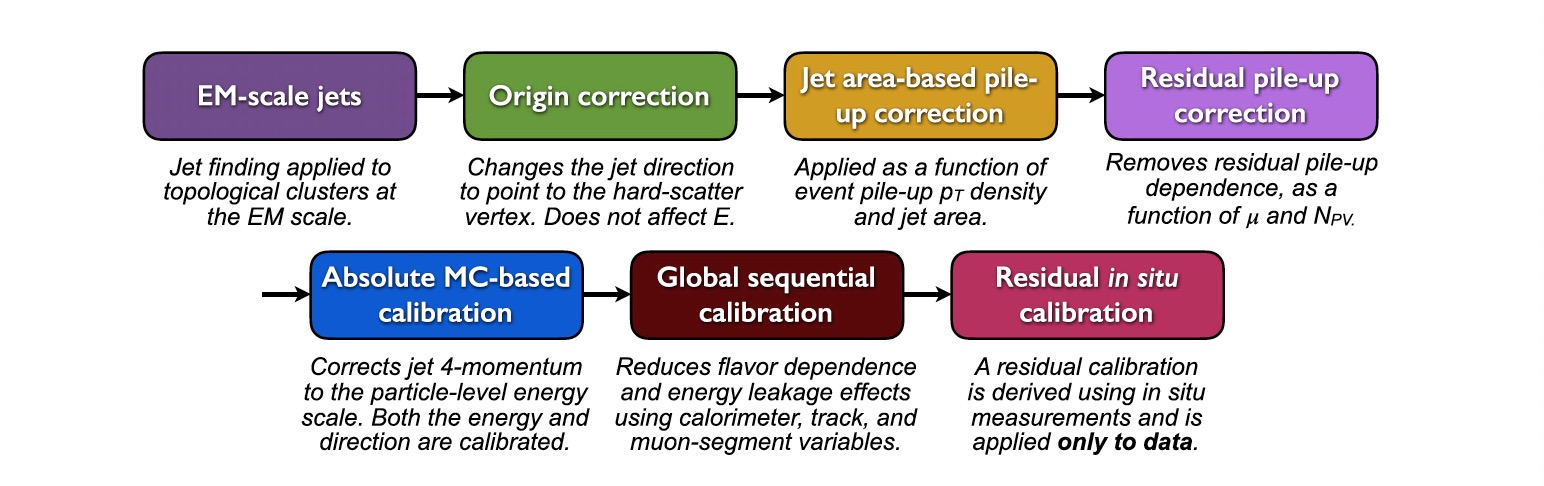
\includegraphics[width=0.9\textwidth]{figuresEXP/ATLASJET3.jpg}
  \end{center}
  \caption{jet能量校准流程图。 }
    \label{fig:ATLASJET3}
\end{figure}



\subsubsection{b-jet}
\label{sec:BJET}

%相对于源于其他夸克的jet来说,来自b夸克的jet具有独特的性质,记为b-jet。
相对于其他类型的jet,来自b夸克的jet具有独特的性质,记为b-jet。
如图~\ref{fig:ATLASBJET1}~所示,b夸克强子化之后,
产生的b强子寿命比较长,约为$1.5\times10^{-12}s$~\cite{PDG},
在ATLAS内部探测器中有明显的飞行距离,
因此可以通过b强子衰变的第二顶点和径迹的碰撞参数来识别b-jet。
%使得可以通过离硬散射主顶点有一小段位移的第二顶点来识别b-jet。
ATLAS合作组中b-jet
%鉴定过程
的标定~\cite{BTAGGING}分为两步,
第一步是重建b-jet中b强子的衰变特征,这个过程包含三个低级算法:
\begin{itemize}
	\item  基于径迹的碰撞参数以它们之间的关联性构建的\textsc{IP2D}和\textsc{IP3D}算法~\cite{IPTD};
	%利用b强子衰变径迹的碰撞参数构建\textsc{IP2D}和\textsc{IP3D}算法~\cite{IPTD};
	\item 基于第二顶点的信息构建的\textsc{SV1}算法~\cite{SVN};
	%用\textsc{SV1}算法~\cite{SVN}重建来自b强子衰变的第二顶点信息;
	\item 算法\textsc{JetFitter}~\cite{JETFT}
	%可以
	用于完整的重建b强子的衰变链。
	%jet中b强子或c强子衰变链,因此可以用于b-jet中b强子衰变链的重建。
	%\item 利用递归神经网络发掘b强子衰变径迹之间的空间和运动学关联性的\textsc{RNNIP}算法~\cite{IPTD};
\end{itemize}
第二步是将这些互补算法的输出合并到一个基于机器学习的高级算法中,
可以得到功能更强大的b-jet标定算法。


\begin{figure}
  \begin{center}
    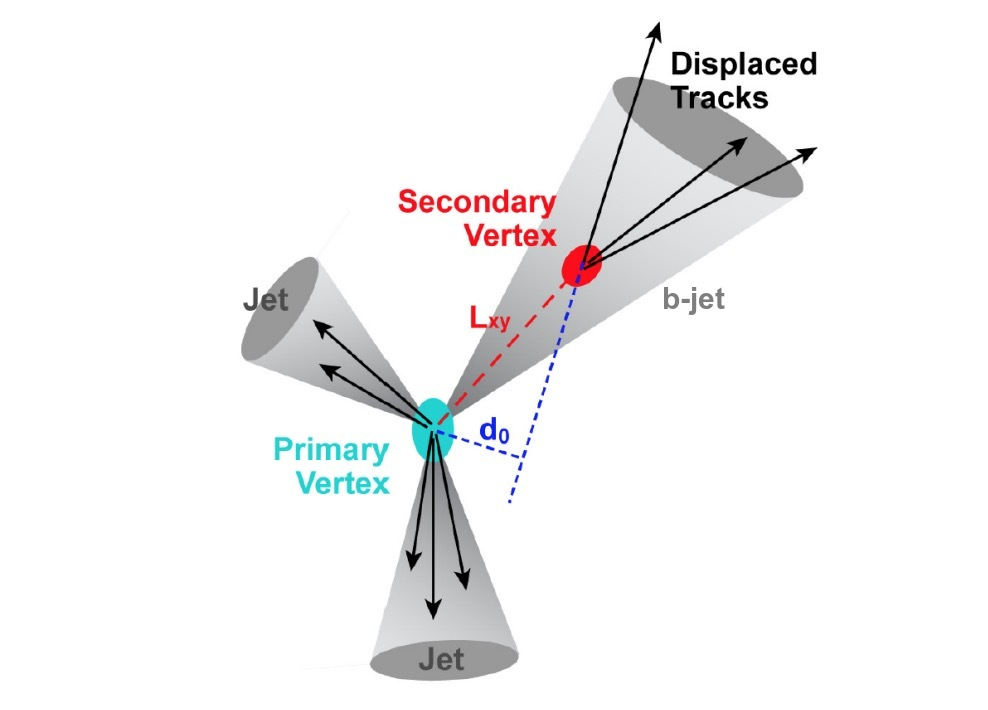
\includegraphics[width=0.75\textwidth]{figuresEXP/ATLASBJET2.jpg}
  \end{center}
  \caption{
b-jet标定示意图。图中红点表示第二顶点,$L_{xy}$表示主顶点和第二顶点的距离,$d_0$是径迹的碰撞参数。
%包含第二顶点的b-jet示意图。
  }
    \label{fig:ATLASBJET1}
\end{figure}


ATLAS合作组常用的两种机器学习算法是提升决策树和神经网络,
这两种机器学习算法将在第~\ref{cha:ML}~章中简要介绍。
%这两种机器学习算法在后续章节~\ref{cha:ML}~有简要介绍。
合并上述三种低级算法的输出并用提升决策树训练出来的b-jet标定算法是MV2~\cite{IPTD}。
而利用神经网络构建
%出来
的b-jet标定算法是DL1~\cite{IPTD}。
%近年来,实现了一种新的利用递归神经网络发掘b强子衰变径迹之间的空间和运动学关联性的低级算法\textsc{RNNIP}算法~\cite{RNNIP},
在2017年,合作组发展了一种基于递归神经网络的低级算法\textsc{RNNIP}~\cite{RNNIP},用于发掘b强子衰变径迹之间的空间和运动学关联性,
DL1r~\cite{DLOR1,DLOR2}是合并上述四种低级算法的输出
并利用神经网络构建的一种新的b-jet标定算法,
由于性能比较好,它是合作组内部推荐的味标定算法,
%也是章节~\ref{cha:Dijet}~中物理分析味标定和章节~\ref{cha:Xbb}~中新算法开发所使用的算法。
也是第~\ref{cha:Dijet}~章中物理分析和第~\ref{cha:Xbb}~章中新算法开发所用到的算法。
%章节~\ref{cha:Xbb}~中新算法与各种算法性能的对比便是用到上述MV2和DL1r两种算法。
另外,b-jet中b强子半轻子衰变产生的$\mu$子对于b-jet的重建也有一定帮助,
SMT(Soft muon tagger)便是基于这个性质构建的另一种低级算法。
%算法SMTnn(Soft muon tagger neural network)便是基于来自重味强子比如b强子或者c强子衰变的$\mu$子的重建而发展出来的一种低级算法,
DL1rmu是结合上述五种低级算法的输出利用神经网络构建的另一种高级算法。
%结合上述五种低级算法的输出用神经网络训练出来的另一种高级算法称为DL1rmu算法。
基于神经网络的高级算法的输出都有三个$p_b$、$p_c$和$p_u$,分别代表jet被判定为b-jet、c-jet或者
%除前两者之外的
light-jet的概率,
其中来自c夸克的jet记为c-jet,来自轻质量夸克比如u、d、s夸克的jet记为light-jet,
c夸克强子化之后,产生的c强子中一部分寿命在$1\times10^{-13}s$~\cite{PDG}的量级,
比b强子寿命短一点,但也可以在探测器中有明显的飞行距离,
而且b强子产生之后有一定概率会衰变成c强子,
因此在探测器中区分b-jet和c-jet是b-jet重建的重要部分。

%寿命比b强子短,大约在
%来自u、d、s夸克的jet记为light-jet,
%其中b-jet作为信号进行训练,另外两种jet作为本底。

\subsection{轻子和光子的重建}
\label{sec:LEPTON}

%电子、光子、$\mu$子和$\tau$子的重建都要依赖内部探测器中重建出来的径迹。
%电子和光子的重建都要依赖内部探测器中重建出来的径迹。
电子的重建是通过内部探测器中
%单个
孤立的径迹与电磁量能器中的拓扑集群之间的匹配实现的~\cite{LEPTON1,LEPTON2,LEPTON3}。
对于光子的重建,
%因为
一部分高能光子会在内部探测器中转化成正负电子对,%而留下径迹,
这部分光子的重建是通过内部探测器中的两条转化径迹与电磁量能器中的拓扑集群之间的匹配实现的,
而另一部分未转化的光子的重建是通过电磁量能器中孤立的拓扑集群实现的,
要求该拓扑集群在内部探测器中没有与之匹配的径迹~\cite{LEPTON2,LEPTON3}。
%因此光子的重建是通过内部两条转化径迹与电磁量能器中的拓扑集群之间的匹配或者
%无匹配径迹的电磁量能器中单个拓扑集群来实现的~\cite{LEPTON2,LEPTON3}。
除了径迹与拓扑集群之间的匹配要求,为了进一步抑制本底,
还要求电磁辐射强度和TRT中的跃迁辐射强度与重建出来的电子和光子的预期表现一致。

$\mu$子的重建是通过内部探测器中的径迹与$\mu$子谱仪中的径迹之间的匹配来完成的,
而内部探测器接收不到的$\mu$子仅由$\mu$子谱仪中的径迹来重建~\cite{LEPTON4,LEPTON5}。
$\tau$子寿命很短,产生之后有65\%的概率以强子末态的形式衰变,35\%的概率衰变成更轻的轻子,
由于
%探测器中
来自轻子型衰变$\tau$子的电子和$\mu$子在探测器中很难与其他过程产生的高能电子和$\mu$子区分开,
因此$\tau$子的重建主要集中在强子型衰变的$\tau$子,它是通过jet重建出来的~\cite{LEPTON6,LEPTON7,LEPTON8}。


\subsection{丢失横动量的重建}
\label{sec:MISSET}

%由垂直于束流轴的平面上的动量守恒,末态所有粒子的横动量矢量和应为零,
由动量守恒,硬散射末态粒子的横动量矢量和为零,
但是由于中微子不能被ATLAS探测到,
%存在不可探测的粒子比如说标准模型中的中微子,
%使得探测器中重建出来的所有末态粒子横动量矢量和不为零,缺失的那部分称为丢失横动量$E_T^{miss}$。
使得探测器中重建出来的部分事例中粒子横动量矢量和不为零,
缺失的那部分即对应产生的中微子的动量,称为丢失横动量$E_T^{miss}$。
丢失横动量的重建过程需要用到探测器中诸多信息~\cite{LEPTON9},
%丢失横动量的重建需要利用到ATLAS探测器中所有子探测器重建出来的信息~\cite{LEPTON9},
它的贡献可以分为两部分:
第一部分是硬贡献项(Hard term),这部分包含
已经重建和校准完成的jet、电子、光子、$\mu$子和$\tau$子;
%已经重建和校准好的jet和粒子比如电子、光子、$\mu$子和$\tau$子;
第二部分是软贡献项(Soft term),
这部分由与硬散射顶点相关联但与硬贡献项不相关的带电粒子径迹组成,
这样做的目的是为了减小来自堆积事例的影响。
考虑上述两部分贡献,
%重建出来的
$E_T^{miss}$是各个贡献项的矢量和的负数:
\begin{equation} 
\label{eq:MISSET}
\begin{split}
E_T^{miss}=&\underbrace{ -\sum_{electrons} p_T^e -\sum_{photons} p_T^{\gamma}  -\sum_{\tau -leptons} p_T^{\tau_{had}}  -\sum_{muons} p_T^{\mu} }_\text{hard term}
\\
&\underbrace{  -\sum_{unused-tracks} p_T^{track} }_\text{soft term}
\end{split}
\end{equation}

















% !TeX root = ../main.tex

\chapter{机器学习}
\label{cha:ML}

LHC上的ATLAS实验接收质子-质子对撞事例的速率约为$1kHz$,每个事例所占的内存大小约为$1.3MB$,这些原始的对撞数据将会被用作后续的粒子重建、校准、分析等工作~\cite{PERF-2007-01}。
而这个大型实验装置的目标主要分为两类,第一个标准模型的精确测量,第二是寻找超出标准模型的新物理,无论哪个目标都要求我们在如此庞大的数据体系中将所需要的信号和本底提取和区分开来。
这就使得机器学习~\cite{RevModPhys.91.045002}能作为一种非常有用的技术手段被应用到高能物理实验(HEP)领域中来,机器学习旨在在大量数据的基础上降低数据的复杂性和发现数据中新的特征,
最早是在十九世纪末二十世纪初,一部分物理学家将简单的前馈神经网络用于事例分类,
而后慢慢的由决策树代替~\cite{JNN62,JNN63,JNN64},这样长达十年之久,从2014年开始,随着深度学习的崛起,
物理学家发现它应用在事例分类等方面相比之前的效果有了显著的提升~\cite{JNN65,JNN66},Baldi等人在2014年将深度学习神经网络第一次用在事例筛选,
用于标定超出标准模型的新粒子,结合MC模拟发现它不仅优于决策树,而且不需要那些精心设计过的事例变量作为输入~\cite{JNN67},
紧接着,他们又引入了参数化的分类器~\cite{JNN68},随后深度学习神经网络接连被用于jet的标定~\cite{JNN69,JNN70,JNN71}和jet味信息的标定~\cite{JNN72},
而且,依赖各种不同的物理模型,不同模式的深度学习神经网络也发展了起来~\cite{JNN73,JNN74,JNN75,JNN76},
除了与jet相关的方面,机器学习在高能物理实验的其他方面都有了比较成功的应用,比如说事例和粒子鉴定、能量分析和堆积事例压低等~\cite{Albertsson_2018}。
而当前高能物理实验领域使用最广的两种机器学习算法是深度学习神经网络(DNN)和提升决策树(BDT),本章将对它们做个概述,读者可以参考书目~\cite{MLTsinghua,MLMIT}详细了解。


\section{神经网络}
\label{sec:NN}

神经网络是一种一般性的多元函数$f:	\mathbb{R}^N\rightarrow\mathbb{R}^M$,将一个代表输入特征的向量$\boldsymbol{x}=(x_1,x_2,	\dots,x_N)$映射到一个有代表性的输出向量$\boldsymbol{y}=(y_1,y_2,	\dots,y_M)$。
这种映射通常可以被用于分类或者回归问题。如图~\ref{fig:BP}所示,这类多元函数是通过用一系列称之为隐层(hidden layers)的结构将输入层$\boldsymbol{x}$(input layers)和输出层$\boldsymbol{y}$(output layers)连接而构建起来的。

\begin{figure}  
  \begin{center}
    \begin{subfigure}{.9\textwidth}
     \centering
    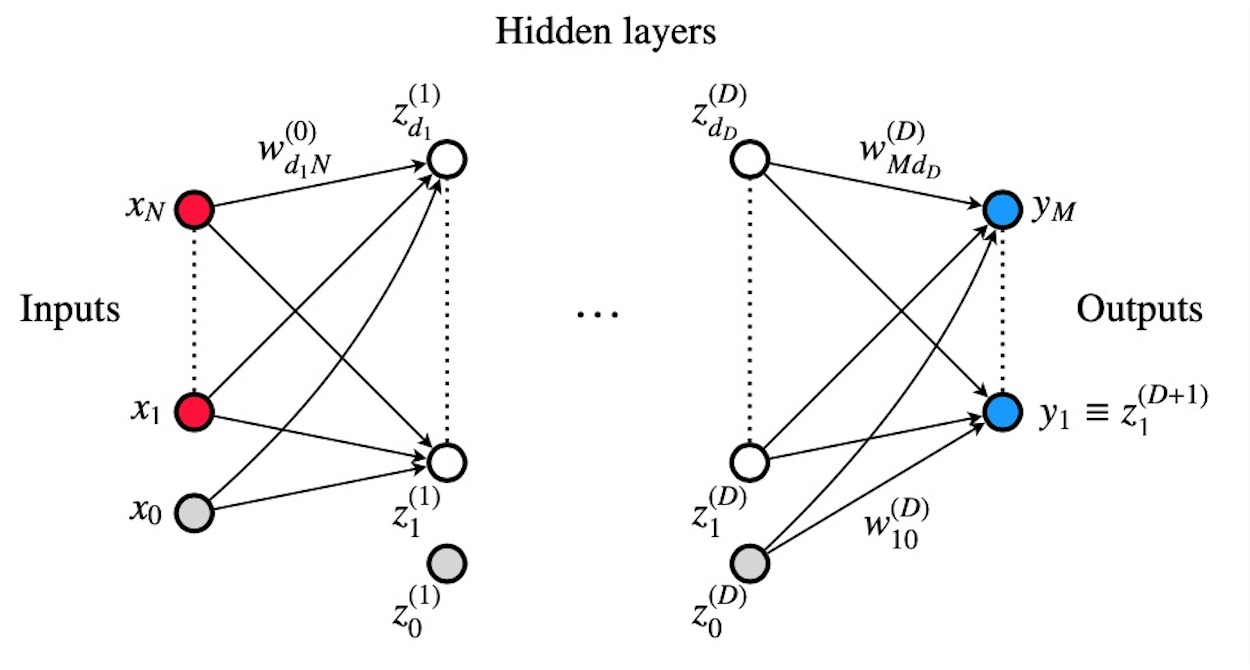
\includegraphics[width=0.75\textwidth]{figuresML/FP.jpg}
    \caption{正向传播过程}
    \end{subfigure}
    \begin{subfigure}{.9\textwidth}
     \centering
    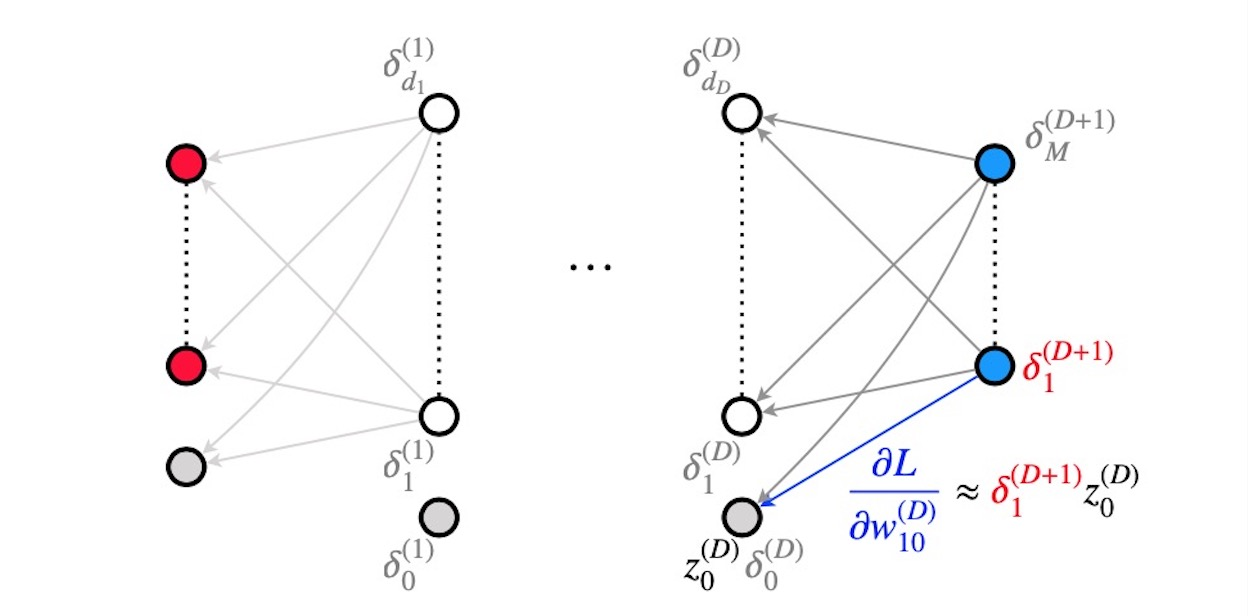
\includegraphics[width=0.75\textwidth]{figuresML/BP.jpg}
    \caption{反向传播过程}
    \end{subfigure}
  \end{center}
  \caption{
前馈(feed-forward)的密集连接型(densely connected)神经网络~\cite{FDNN}示意图。每个节点代表一个输入或者输出,每条线代表一个权重因子。反向传播算法的学习过程由(a)和(b)两个过程组成。
  }
  \label{fig:BP}
\end{figure}

相邻层之间的连接是通过一个线性变换和一个非线性的激活函数$h:\mathbb{R}^N\rightarrow\mathbb{R}^M$(activation function)实现的:
\begin{equation} 
\label{eq:ml1}	
a_{i}^{(l+1)}=\sum_{j=1}^{d_l} w_{ij}^{(l)}z_{j}^{(l)} + b_{i}^{(l)} = \sum_{j=0}^{d_l} w_{ij}^{(l)}z_{j}^{(l)}, \quad z_{i}^{(l)}=h(a_{i}^{(l)})
\end{equation}
其中,$l$是层指标,$\boldsymbol{z}^{(l)}={z_{i}^{(l)}}$是第$l$层中每个被称为节点(node)的值,$d_l=\|\boldsymbol{z}^{(l)}\|$是第$l$层中总的节点数目,$\boldsymbol{W}^{(l)}={w_{ij}^{(l)}}$是$d_{l+1} \times d_l$权重矩阵,
$\boldsymbol{b}^{(l)}={b_{i}^{(l)}}$是长度为$\|\boldsymbol{b}^{(l)}\|=d_{l+1}$的偏移向量,$\boldsymbol{a}^{(l)}={a_{i}^{(l)}}$是第$l$层中节点的线性组合或者输出,作为非线性激活函数的输入。输入和输出层分别对应于$\boldsymbol{x}=\boldsymbol{z}^{(0)}$和$\boldsymbol{y}=\boldsymbol{z}^{(D+1)}$。这里将神经网络的整个参数集记为$\theta$。

神经网络的体系结构是由隐层和每个隐层的节点配置所决定的,通常会被作为训练阶段的一部分得到优化。
每个附加的隐层和隐层中每个附加的节点都会为神经网络增加可调参数,从而增加神经网络的容量。这就使得神经网络能近似成任意复杂的连续函数。通常,神经网络也被称为通用型估计器(universal approximators),这意味着,在容量足够的情况下,它能以任意的精度近似成任意的连续函数~\cite{MLSV}。因此,在用于调整神经网络参数的数据集足够大的情况下,这个性质使得它非常适合复杂的计算任务。


\subsection{训练}
\label{sec:Train}

到此,我们介绍了神经网络的基础,其中信息流是以输入到输出的方式前向传播的。接着,比较关键的一个概念是对神经网络的训练,即针对一个特定的分类或者回归任务,调整网络的结构参数$\theta$,这便是机器学习中“学习”的过程。
在训练开始的时候,网络的结构参数$\theta$不是已知的,通常是从某个分布比如说高斯分布中随机取样进行初始化的。
在标准的$\chi^2$回归分析法~\cite{WENDT1991275}当中,可以精确的计算目标函数相对于每个拟合参数的梯度,从而可以使用一定的梯度下降算法来最小化目标函数。
然而对于神经网络,可能有数百万个结构参数,从而参数空间维数太大,使得上述方法不可行,因此需要一种新的方法来实现网络的结构参数调节。

与函数优化相似的是,神经网络的训练是通过最小化某个特定任务的目标函数,或者被称为损失函数(loss funcion)$L$来实现的。

对于回归任务,在给定输入集$X$和目标集$Y$的情况下,损失函数是均方差(MSE):
\begin{equation} 
\label{eq:ml2}	
L_{MSE}(\theta) = \mathbb{E}_{\boldsymbol{x} \sim X, \boldsymbol{y} \sim Y} \left[ \frac{1}{M} \sum_{i=1}^M (y_i - p_i (\boldsymbol{x} \mid \theta))^2 \right]
\end{equation}
其中$\mathbb{E}$表示一组相关联的输入集和回归目标的平均,$\theta$是神经网络的结构参数集,$p_i (\boldsymbol{x} \mid \theta)$是给定结构参数集$\theta$条件下神经网络对应于输入集$\boldsymbol{x}$的第$i$个预测输出。这个损失函数是神经网络的预测输出与相对应的回归目标之间的平均欧式距离。

对于带有关联标记$y\in\{[1,0,0],[0,1,0],[0,0,1]\}$的输入集$\boldsymbol{x}$的多分类任务,在神经网络的最后一层通常会使用\textsc{SoftMax}~\cite{MLMIT}作为激活函数,用以确保将神经网络的三个输出变量都限制在开区间$(0,1)$内。
这种情况下,可以使用多分类交叉熵(categorical cross-entropy,CCE)作为损失函数:
\begin{equation} 
\label{eq:ml3}	
L_{CCE}(\theta) = \mathbb{E}_{\boldsymbol{x} \sim X, \boldsymbol{y} \sim Y} \left[ - \sum_{i=1}^3 (y_i log p_i (\boldsymbol{x} \mid \theta)) \right]
\end{equation}
同样,这里$p(\boldsymbol{x} \mid \theta)$是给定结构参数集$\theta$条件下神经网络对应于输入集$\boldsymbol{x}$的预测输出。
此处的多分类交叉熵对应于体系的似然函数的对数的负数值,因此可以将其理解为在给定结构参数集$\theta$和输入集$\boldsymbol{x}$情况下标记$y$出现的概率~\cite{MLSV}。


\subsection{反向传播算法}
\label{sec:BackProp}

在根据式~\ref{eq:ml2}或~\ref{eq:ml3}中损失函数来训练神经网络时,由于参数空间维数太大,需要一种不依赖结构参数空间中每个参数独立变化的方法来估计梯度$\partial L / \partial w_{ij}^{(l)}$。
因为式~\ref{eq:ml1}中带有$D$个隐层的标准神经网络就是$D+1$个非线性可微函数的组合,那么,微积分中的链式法则可以被用来估计梯度,从而可以用近似梯度下降算法来训练神经网络。

在一个密集连接型神经网络~\cite{DenNet}中,式~\ref{eq:ml1}中$a^{(l-1)}$的变化是通过它们与$a^{(l)}$的连接而引起$L_{MSE}$或$L_{CCE}$的变化。如图~\ref{fig:BP},中间输出层$a^{(l)}$也直接依赖于第$l$层中的权重因子$w_{ij}^{(l-1)}$。由于神经网络中所有线性变换以及损失函数相对于线性变换中的权重都是可微的,因此可以在此处用到链式法则:
\begin{equation} 
\label{eq:BP1}	
\frac{\partial L}{\partial w_{ij}^{(l)}} \bigg\rvert_{\{\boldsymbol{x},\boldsymbol{y}\}} \equiv \frac{\partial L}{\partial w_{ij}^{(l)}} \equiv \underbrace{\frac{\partial L}{\partial a_{i}^{(l+1)}}}_{\equiv \delta_{i}^{(l+1)}} \frac{\partial a_{i}^{(l+1)}}{\partial w_{ij}^{(l)}} = \delta_{i}^{(l+1)}z_{j}^{(l)}
\end{equation}
其中$\delta_{i}^{(l+1)}$是为代替$\frac{\partial L}{\partial a_{i}^{(l+1)}}$而引入的缩写,称之为误差,右边第二项由式~\ref{eq:ml1}得到。
这就表示,损失函数相对于权重因子的梯度是由输入节点的值和这个权重因子所连接的误差决定的,如图~\ref{fig:BP}所示。
这种梯度计算方法和依赖关系适用于任意一组输入集$\boldsymbol{x}$和目标集$\boldsymbol{y}$。
为了方便起见,可以利用链式法则进一步对隐层中的误差进行分解:
\begin{equation} 
\label{eq:BP2}	
\delta_{i}^{(l)}=\frac{\partial L}{\partial a_{i}^{(l)}}=\sum_k \underbrace{\frac{\partial L}{\partial a_{k}^{(l+1)}}}_{= \delta_{k}^{(l+1)}} \underbrace{\frac{\partial a_{i}^{(l+1)}}{\partial a_{i}^{(l)}}}_{= w_{ki}^{(l)}h' \left( a_{i}^{(l)} \right) } \approx h' \left( a_{i}^{(l)} \right) \sum_k \delta_{k}^{(l+1)} w_{ki}^{(l)}
\end{equation}
这里再次用到了式~\ref{eq:BP1}中误差的定义和式~\ref{eq:ml1},其中$h'$是激活函数的一阶微分。式~\ref{eq:BP2}将第$l$层每个节点的误差和第$l+1$层节点的误差联系了起来。初始条件由含$D$个隐层的神经网络的输出层$l=D+1$的误差给出:
\begin{equation} 
\label{eq:BP3}	
\delta_{i}^{(D+1)}=\frac{\partial L}{\partial a_{i}^{(D+1)}}= \frac{\partial L}{\partial z_{i}^{(D+1)}} \frac{\partial z_{i}^{(D+1)}}{\partial a_{i}^{(D+1)}} = \frac{\partial L}{\partial p_{i}} h' \left( a_{i}^{(D+1)} \right)
\end{equation}
通过递归运用式~\ref{eq:BP3}可以将误差从输出层$l=D+1$反向传播到输入层$l=0$,
给定这些误差之后,损失函数相对于神经网络中各个权重因子的微分由式~\ref{eq:BP1}给出。
因此,对于每个输入集$\boldsymbol{x}$和对应的目标集$\boldsymbol{y}$,最简单的情况是通过以下方法更新神经网络中的权重,从而达到最小化损失函数的目的:
\begin{equation} 
\label{eq:BP4}	
w_{ij}^{(l)} \leftarrow w_{ij}^{(l)} - \eta \frac{\partial L}{\partial w_{ij}^{(l)}} \bigg\rvert_{\{\boldsymbol{x},\boldsymbol{y}\}} = w_{ij}^{(l)} - \eta \delta_{i}^{(l+1)}
\end{equation}
其中$\eta$是学习速率,用于控制每次权重更新的尺度,从而控制随机梯度下降(stochastic gradient descent)的速率。通过迭代权重更新式~\ref{eq:BP4},可以在训练神经网络时实现最小化损失函数$L(\theta)$。


\section{提升决策树}
\label{sec:BDT}

决策树(Decision tree, DT)~\cite{BDT2,BDT1}是另一种机器学习算法。
与神经网络类似,它可以将一个N维特征输入向量$\boldsymbol{x}=(x_1,x_2,	\dots,x_N)$映射到一个代表特征类的概率值或一个函数值,
这取决于具体任务是分类问题还是回归问题。
这里以二进制分类(binary classification)问题为例来具体说明。
为了构建二进制决策树,标准的分类和回归决策树算法(The standard classification and regression tree, CART)
通过在单个特征上进行二进制筛选来顺序划分输入特征空间。
首先,决策树从包含整个训练数据的单个节点开始,这个起始节点被称为根节点R,
在最简单的情况下,任务会对数据进行一次拆分,使得数据被最优地分为两个类,成为两个部分,
分类之后会出现两个子节点N,分别代表被分开的两部分。
为了找到最佳分类,算法会对每个特征输入$\boldsymbol{x}$进行扫描,
并根据代表具体任务的某些度量来评估该分割,一种常用的度量称为基尼指数~\cite{BDT1}。

在根节点进行第一次拆分之后,这个拆分过程会递归应用到每个子节点上面,
根据具体任务,每次拆分都会使得局部类纯度最大化。
这种顺序的二进制拆分会形成一个“二进制树”,
其中每个内部节点都对应一个特定的决策,因此被命名为“决策树”。
后续的每一步都是为了提高类纯度,
当训练数据中每个样本都被正确的归类或者达到某些停止条件的时候,
拆分便会停止,比如限制决策树的最大节点层数。
分类结束后,决策树的最后一层节点称为叶节点,
从根节点到叶节点的每条路径称为分支。
决策树中的这些属性便是其结构参数,会根据每个实际的任务得到优化。
图~\ref{fig:BDT}~展示的是一个简单的二进制决策树及其特征空间划分示例。

\begin{figure}
  \begin{center}
    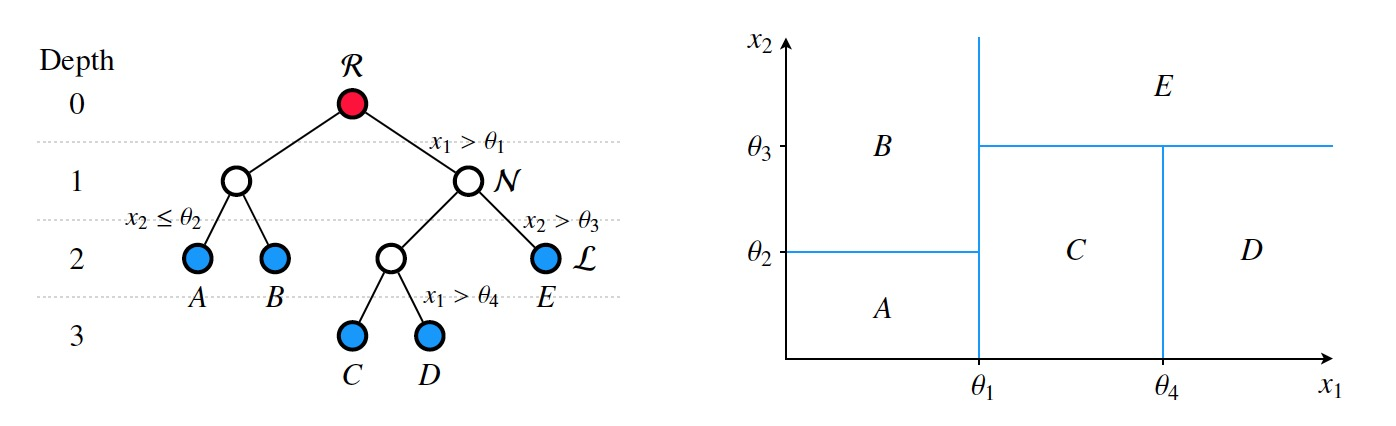
\includegraphics[width=0.9\textwidth]{figuresTHE/BDT.jpg}
  \end{center}
  \caption{二维特征输入$\boldsymbol{x}=(x_1,x_2)$的二进制决策树示例(左图),其中包含一个根节点、三个决策节点和五个叶节点将
  输入特征空间分为五个不相交的决策区间(右图)。 }
    \label{fig:BDT}
\end{figure}

在单个决策树中,每个叶节点表示的特征子空间内的样本将具有相同的预测输出值,
对于分类问题,预测值是叶节点上每个相同类上的训练样本所占的比例,
而对于回归问题,预测值是目标函数的平均值。
从这里可以看出决策树的决策功能不连续,
这对于大多数关系都是连续的高能物理领域来说是不理想的,
于是在此基础上引入了称为提升的方法。
该方法的出发点是通过组合一系列较弱的学习本领而得到一个较强的学习本领,

提升决策树(Boosted decision trees, BDT)~\cite{BDT3,BDT4}算法会按顺序训练一系列的决策树,记为提升梯级t。
在每个提升梯级中,分配给在上一梯级中修改过的每个训练样本的权重都会增加,
从而增加它的重要性。
然后根据提升梯级中t中错误分类的训练样本的加权比例来计算一个决策树权重$a^t$,
最后通过加权平均将所有的决策树组合在一起:
\begin{equation} 
\label{eq:BDT}
BDT(\boldsymbol{x})=\sum_t a^t DT^t(x) 	
\end{equation}
通过这种决策树的提升方法,可以得到一个更强大的提升决策树算法,
它能为样本进行更好的分类,而且不容易过拟合,也不会像单个决策树那样出现决策不连续的问题。


































% !TeX root = ../main.tex

\chapter{高横动量希格斯玻色子衰变到双b夸克的标定}
\label{cha:Xbb}


自从ATLAS实验和CMS实验在2012年发现希格斯玻色子~\cite{ATLASHIGGS,CMSHIGGS}之后,与之相关的一系列性质的精确测量变得非常重要,比如其自身性质、它与标准模型中其他粒子的耦合和它的产生模式和衰变,
这些属性都能对标准模型进行严格验证。
而这也是LHC上两个大型探测器ATLAS和CMS的主要任务之一,
在2015年到2018年$Run\_2$计划期间,LHC将质心系能量提高到了13TeV,ATLAS探测器和CMS探测器在这期间收集到的可用于物理分析的数据总积分亮度分别为139$fb^{-1}$和137$fb^{-1}$,
并开展一系列与希格斯玻色子相关的研究,标准模型中希格斯玻色子的产生和衰变在第~\ref{sec:Higgs}~小节中有简要介绍,
这里在表~\ref{tab:ACHIGGS}~中总结了ATLAS实验和CMS实验进行的与希格斯玻色子产生和衰变相关的一系列最新测量结果~\cite{ATLASHM,CMSHM},
ATLAS合作组和CMS合作组测得的组合希格斯玻色子信号强度
$\footnote{组合信号强度定义为测得的信号量与标准模型所预测的信号量的比值。}$分别为1.06$\pm$0.07和$1.02^{+0.07}_{-0.06}$,
并且由不同产生和衰变模式测得的信号强度都与标准模型的预期一致。

%ATLASHIGGS\cite{ATLASHIGGS1,ATLASHIGGS2,ATLASHIGGS3,ATLASHIGGS4,ATLASHIGGS5,ATLASHIGGS6,ATLASHIGGS7}
%CMSHIGGS\cite{CMSHIGGS1,CMSHIGGS2,CMSHIGGS3,CMSHIGGS4,CMSHIGGS5,CMSHIGGS6,CMSHIGGS7,CMSHIGGS8,CMSHIGGS9,CMSHIGGS10}
%ATLASHBB\cite{AHbb1,AHbb2,AHbb3,AHbb4,AHbb5,AHbb6,AHbb7,AHbb8,AHbb9}
%CMSHBB\cite{CHbb1,CHbb2,CHbb3,CHbb4}

\begin{table}[ht]
\caption{ATLAS实验和CMS实验进行的与希格斯玻色子产生和衰变相关的一系列最新测量结果。}
\begin{center}
\begin{adjustbox}{width=\columnwidth,center}
\begin{tabular}{c|cc|cc}
    \hline
    \hline
    \multirow{2}{*}{Analysis} & \multicolumn{2}{c|}{ATLAS} & \multicolumn{2}{c}{CMS} \\
    & Production tags & \thead{Luminosity($fb^{-1}$) \\ and References} & Production tags & \thead{Luminosity($fb^{-1}$) \\ and References} \\
    \hline
    $H\rightarrow\gamma\gamma$ & \thead{ggF,VBF,WH\\ZH,$t\bar{t}H$,tH} & 139\cite{ATLASHIGGS1} & ggF,VBF,$t\bar{t}$H & 35.9\cite{CMSHIGGS2},41.5\cite{CMSHIGGS3},77.4\cite{CMSHIGGS1} \\
    \hline
    $H\rightarrow ZZ^*$ & \thead{ggF,VBF,WH\\ZH,$t\bar{t}H$,tH} & 36.1\cite{ATLASHIGGS5,AHbb10},139\cite{ATLASHIGGS2} & \thead{ggF,VBF,VH\\$t\bar{t}H$}& 137\cite{CMSHIGGS4}  \\
     \hline
    $H\rightarrow WW^*$ & ggF,VBF,$t\bar{t}H$ & 36.1\cite{ATLASHIGGS3,ATLASHIGGS5,AHbb10} & \thead{ggF,VBF,VH\\WH,ZH} & 35.9\cite{CMSHIGGS5}  \\
     \hline
    $H\rightarrow \tau\tau$ & ggF,VBF,$t\bar{t}H$ & 36.1\cite{ATLASHIGGS4,ATLASHIGGS5,AHbb10} & ggF,VBF,VH & 35.9\cite{CMSHIGGS6},77.4\cite{CMSHIGGS7}   \\
     \hline
    $H\rightarrow b\bar{b}$ & \thead{VBF,WH,ZH\\$t\bar{t}H$}  & 30.6\cite{AHbb6},36.1\cite{AHbb7,AHbb8},139\cite{AHbb5} & \thead{ggF,WH,ZH\\$t\bar{t}H$} & 35.9\cite{CHbb3},41.5\cite{CHbb2,CHbb4},77.4\cite{CHbb1} \\
     \hline
    $H\rightarrow \mu\mu$ & \thead{ggF,VBF,VH\\$t\bar{t}H$} & 139\cite{ATLASHIGGS6} & ggF,VBF& 35.9\cite{CMSHIGGS10}  \\
    \hline
    \hline
\end{tabular}
\end{adjustbox}
\end{center}
\label{tab:ACHIGGS}
\end{table}

其中,尽管$H\rightarrow b\bar{b}$衰变道是希格斯玻色子的主要衰变模式,占高达$58\%$的分支比,
但是也因为来自QCD过程和t夸克衰变的本底非常大,使得在LHC上面观测这个衰变模式变得很困难。
通过要求事例中包含孤立的轻子,可以显著的降低QCD本底,因此寻找$H\rightarrow b\bar{b}$衰变道灵敏度最高的产生模式是VH,
ATLAS合作组和CMS合作组在2018年分别利用$79.8fb^{-1}$和$41.3fb^{-1}$的数据通过VH产生模式观测到显著的$H\rightarrow b\bar{b}$事例,
显著性分别达到了4.9和4.8倍的标准差~\cite{AHbb8,CHbb3},
随后在2020年,ATLAS合作组利用$139fb^{-1}$的数据观测到了更加丰富的事例~\cite{AHbb5}。
但是也有一部分研究在其他产生模式下测量$H\rightarrow b\bar{b}$的衰变,比如$t\bar{t}H$~\cite{AHbb7,AHbb8,CHbb1}、VBF~\cite{AHbb6}和高横动量区的ggF~\cite{CHbb3}。

而高横动量的$H\rightarrow b\bar{b}$衰变与低横动量的$H\rightarrow b\bar{b}$衰变拓扑性质不一样,
如图~\ref{fig:Boosted}~所示,在探测器中,来自高横动量希格斯玻色子衰变的两个b夸克接近准直,
会合并到一个LR-jet当中,依靠其整体性使得$H\rightarrow b\bar{b}$事例更容易鉴定。
而且在许多超出标准模型的新物理模型中~\cite{BSMHIGGS1,BSMHIGGS2,BSMHIGGS3}都引入了能与标准模型中希格斯玻色子耦合的新粒子的存在,
这些新粒子的质量都很大,衰变产生的希格斯玻色子将会具有很高的横动量。
因此对高横动量的$H\rightarrow b\bar{b}$衰变的研究或者标定对希格斯玻色子性质的精确测量和新物理的寻找都有着重要意义。

\begin{figure}
  \begin{center}
    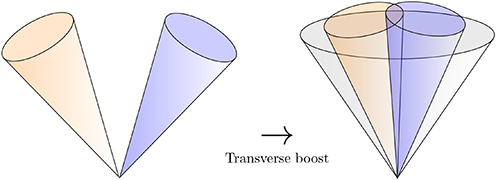
\includegraphics[width=0.75\textwidth]{figuresXbb/Boosted.jpg}
  \end{center}
  \caption{
来自高横动量希格斯玻色子衰变的两个b夸克接近准直,从而合并到一个LR-jet当中。
  }
    \label{fig:Boosted}
\end{figure}



\section{研究背景}
\label{sec:XbbBKG}


%TAGGING~\cite{TAGGING1,TAGGING2,TAGGING3,TAGGING4}
ATLAS合作组早在2014年就开始研究强子型衰变的LR-jet标定算法。
包括高横动量的希格斯玻色子的标定,最早在2014年它是利用LR-jet中subjet基于提升决策树的高级算法实现对LR-jet的标定的,并优化了距离参数R~\cite{TAGGING1},
随后在$Run\_2$计划期间合作组沿用了这一标定方法并开始使用优化后的距离参数R~\cite{TAGGING5},
并且后续为了更好的提高高横动量希格斯玻色子标定的性能,合作组还发展了专用的subjet重建算法~\cite{ATL-PHYS-PUB-2017-010}。
而在2015年左右高横动量的W玻色子~\cite{TAGGING3}和t夸克(Top)的标定~\cite{TAGGING2}中,
它们利用了LR-jet整体的独特性质发展了一系列低级算法和相应的变量(Jet substructure, JSS)用于LR-jet的标定,
称为LR-jet的结构变量,
表~\ref{tab:JSS}~总结了这些标定技术和对应的变量,第~\ref{sec:XbbORJSS}~小节将对它们做简要介绍。

\begin{table}[ht]
\caption{用于高横动量W玻色子和t夸克标定的各种低级算法和对应的变量。称为LR-jet的结构变量。}
\begin{center}
\begin{adjustbox}{width=\columnwidth,center}
\begin{tabular}{c|c|c}
    \hline
    \hline
    Observable & Variable & Tagging and reference \\
    \hline  
    Energy correlation ratios & \thead{$ECF_1,ECF_2$\\$ECF_1,C_2,D_2,e_3$} & t,W\cite{JSS1,JSS2} \\
    \hline  
    N-subjettiness & \thead{$\tau_1,\tau_2,\tau_3$\\$\tau_{21},\tau_{32}$} & t,W\cite{JSS3,JSS4} \\
    \hline  
    Center of mass observables & \thead{Fox Wolfram($R_2^{FW}$)\\Sphericity(S)\\Thrust($T_{MIN},T_{MAJ}$)} & W\cite{JSS5,JSS6,JSS7}  \\
    \hline  
    Splitting Measures & \thead{$Z_{CUT12},\mu_{12}$\\$\sqrt{d_{12}},\sqrt{d_{23}}$} & \thead{W\cite{JSS8,JSS9}\\t,w\cite{JSS10}} \\
    \hline  
    Planar Flow & $\mathcal{P}$& W\cite{JSS11} \\
    \hline  
    Dipolarity & $\mathcal{D}$ & W\cite{JSS12} \\
    \hline  
    Angularity & $a_3$ & W\cite{JSS13} \\
    \hline  
    Aplanarity & $A$ & W\cite{JSS6} \\
    \hline  
    KtDR & $KtDR$ & W\cite{JSS14} \\
    \hline  
    Qw & $Q_w$ & W\cite{JSS8} \\
    \hline
    \hline
\end{tabular}
\end{adjustbox}
\end{center}
\label{tab:JSS}
\end{table}


后来合作组利用神经网络和提升决策树将这些变量整合到更高级的LR-jet标定算法当中~\cite{ATL-PHYS-PUB-2017-004},
使得标定效率有了显著提升,但是随之而来也引入了一个困难,
如图~\ref{fig:MSCULP}~所示,
其中绿色实线表示QCD样本中LR-jet的质量分布,
而深红色虚线表示被基于神经网络的高级算法标定之后的LR-jet质量分布,
蓝色虚线表示被基于提升决策树的高级算法标定之后的LR-jet质量分布。
可以看到基于神经网络和提升决策树的高级算法学会了利用LR-jet质量信息区分信号和本底,
也就是在被高级算法标定后,QCD样本中的LR-jet的质量分布会失真,并变成类似于W玻色子的质量分布,
使得这种高级算法与LR-jet的质量表现出非常大的非线性相关性,
这在实际的利用质量谱测定散射截面或寻找新物理的分析中是不允许出现的。

\begin{figure}
  \begin{center}
    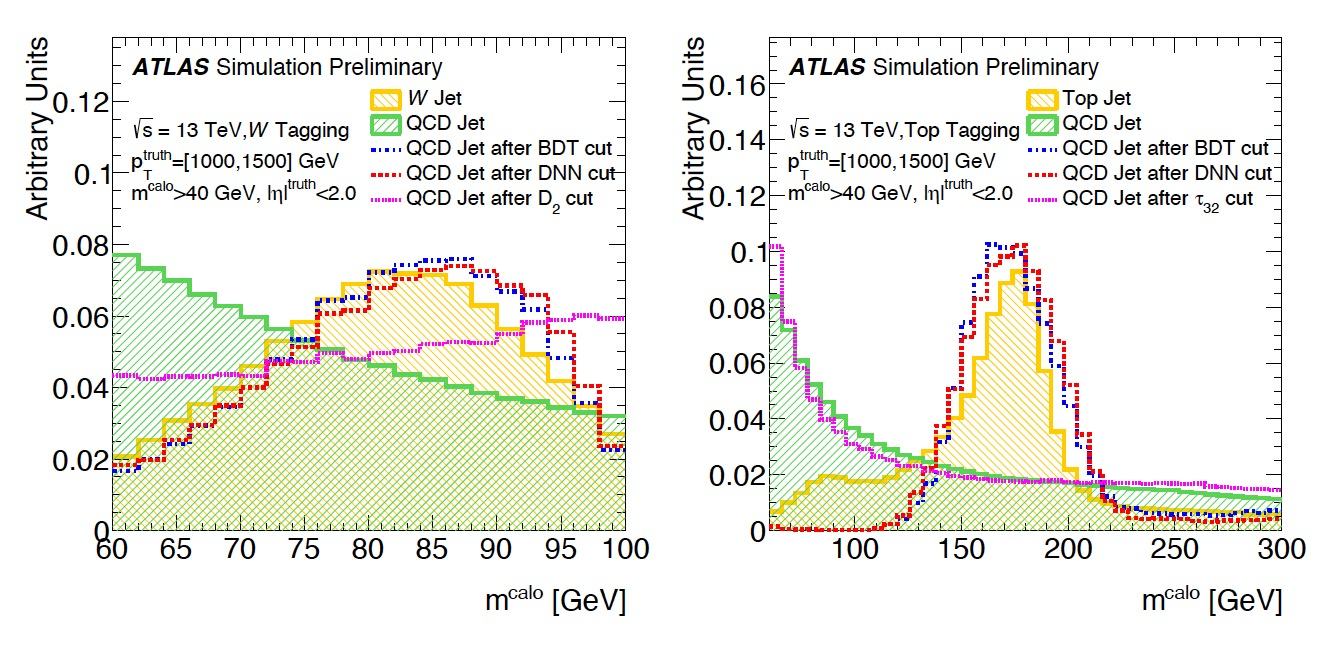
\includegraphics[width=0.9\textwidth]{figuresXbb/MSCULP.jpg}
  \end{center}
  \caption{
基于神经网络(DNN)和提升决策树(BDT)的高级算法标定前和标定后,信号和本底的LR-jet质量分布。
左图是W玻色子标定,右图为t夸克标定。
  }
    \label{fig:MSCULP}
\end{figure}



针对这一问题,合作组在2018年提出了多种去质量关联的技术~\cite{ATL-PHYS-PUB-2018-014}:
专用去相关标定算法(Designed decorrelated taggers, DDT)~\cite{DDT}、
k近邻回归方法(Fixed-efficiency k-nearest neighbours regression, k-NN)~\cite{KNN}和
卷积结构方法(convolved substructure, CSS)~\cite{CSS}
提供了三种解除JSS与LR-jet质量之间关联性的解析方法;
而对抗性神经网络(adversarial neural networks, ANN)~\cite{ANN}和
自适应增强方法(adaptive boosting for uniform efficiency, uBoost)~\cite{UBOOST}则是
通过降低基于机器学习的高级算法与LR-jet质量之间的相关性来解决这个问题。
其中基于对抗性神经网络的算法能成功的实现去质量关联性,但是是以牺牲精确度为代价,
图~\ref{fig:ANNROC}~展示的是对于上述几种去质量关联的算法,
来自W玻色子的信号jet标定效率\footnote{效率定义为算法标定的物理对象数目与用到的物理对象总数的比值。}
与来自QCD过程的本底排除率\footnote{排除率定义为用到的物理对象总数与算法标定的物理对象数目的比值。}
的关系,
左图为低横动量区间[200,500]GeV,右图为横高动量区间[500,1000]GeV,
不同颜色的虚线对应不同的去质量关联算法,
在信号效率相等的情况下,本底排除率越高说明算法的性能越好,
可以看到,
基于对抗性神经网络的去质量关联算法$Z_{ANN}$相对于基于神经网络的表现出质量相关性的算法$Z_{NN}$来说,
存在一定程度的性能损失。


\begin{figure}
  \begin{center}
    \includegraphics[width=0.9\textwidth]{figuresXbb/ANN.jpg}
  \end{center}
  \caption{对于不同的去质量关联算法~\cite{ATL-PHYS-PUB-2018-014},来自W玻色子的信号jet标定效率与来自QCD过程的本底排除率的关系。
其中LR-jet质量满足m$\in$[600,1000]GeV,左图为低横动量区间[200,500]GeV,右图为横高动量区间[500,1000]GeV。}
    \label{fig:ANNROC}
\end{figure}


同时,在高横动量的希格斯玻色子标定方面,
合作组希望结合之前沿用的技术即基于LR-jet中subjet的标定算法和高横动量的W玻色子和t夸克的标定技术,
发展一种基于神经网络的既能实现去质量关联又能保持高精确度的高级算法。
但在经过两轮研究人员的尝试之后,发现始终不能同时保证去质量关联和高精确度,
我在2019年初接手这个任务之后,在尝试原有方法不可行的同时,也开始尝试新方法,
最后成功发展出一种既能实现去质量关联又能保持高精确度的高级算法。

本章将要展示的是,基于前馈型深度学习神经网络~\cite{FDNN}和变量控制的方法,利用LR-jet的运动学变量和其中subjet的高级标定算法,
实现了一种既能实现去质量关联又能保持高精确度的高横动量$H\rightarrow b\bar{b}$标定算法。

\section{MC样本}
\label{sec:XbbSim}

\subsection{信号}
\label{sec:XbbSimS}

为了产生丰富的信号事例,
高横动量的希格斯玻色子是由MC模拟的超出标准模型的Randall-Sundrum额外维模型~\cite{Randall:1999ee}产生,
模型中的Kaluza-Klein引力子能与标准模型中希格斯玻色子耦合,其中耦合参数被设置为$k/\bar{M}_P=1$,
并衰变到两个希格斯玻色子,希格斯玻色子的质量设置为125GeV,
两个希格斯玻色子随后均衰变为$b\bar{b}$夸克对。
事例是使用领头阶NNPDF2.3部分子分布函数~\cite{Martin:2009iq}和\textsc{ATLAS A14}校准参数集~\cite{ATL-PHYS-PUB-2014-021}
并通过\textsc{Pythia 8.186}~\cite{Sjostrand:2007gs}和\textsc{MadGraph5}~\cite{Alwall:2014hca}模拟产生。
Kaluza-Klein引力子和希格斯玻色子之间的质量差距足够大的情况下可以迫使衰变出来的希格斯玻色子具有高横动量,
因此,这里模拟到的Kaluza-Klein引力子质量有:300、400、500、600、700、800、900、1000、1100、1200、1300、1400、1500
、1600、1800、2000、2250、2500、2750、3000、3500、4000、4500、5000、6000GeV,
可以使信号样本以合适的比例覆盖感兴趣的高横动量区域,这些MC样本中,希格斯玻色子只衰变到$b\bar{b}$夸克对。
各个引力子质量不同的样本最后会合并在一起并且重新赋予权重,使得其中LR-jet的横动量分布和QCD样本中的一致,
用于后续算法性能的评估和对比,
下一小节也就是第小节将会介绍其中一种本底高横动量的QCD过程的模拟。
这样加权是为了减小由未加权的样本之间的运动学差异带来的影响。


\subsection{本底}
\label{sec:XbbSimB}

这里考虑了两种本底:一种是来自QCD过程高横动量的夸克胶子相互作用或胶子自相互作用,记为multijet,
模拟的multijet样本中事例的领头LR-jet也就是横动量最高的LR-jet的横动量分布如图~\ref{fig:bkg-pt}~所示,
具有这种物理分布的样本会用于第~\ref{sec:XbbTagger}~小节和第~\ref{sec:XbbPerf}~小节中算法性能的评估和对比;
另一种是来自于强子型衰变的高横动量t夸克的LR-jet,
为了产生丰富的t夸克事例,
t夸克样本是由$Z\prime$模型中高质量$Z' \to t\bar{t}$衰变产生,
所模拟的$Z\prime$质量有:
400、500、750、1000、1250、1500、1750、2000、2250、2500、2750、3000、4000、5000GeV。
同样,所有样本最后会合并在一起并且重新加权,使得最后LR-jet的横动量分布和QCD样本中的一致,
而且这些MC样本中,t夸克只允许强子型衰变。
这两种本底样本都是使用领头阶NNPDF2.3部分子分布函数和\textsc{ATLAS A14}校准参数集
并通过\textsc{Pythia 8.186}~\cite{Sjostrand:2007gs}模拟产生的。

\begin{figure}
  \begin{center}
    \includegraphics[width=0.75\textwidth]{figuresXbb/samples/pt_norm.pdf}
  \end{center}
  \caption{
  multijet样本中LR-jet的横动量分布。分布已经被归一化。
  }
    \label{fig:bkg-pt}
\end{figure}

所有样本中的堆积事例都是用\textsc{Pythia 8}来实现的,
事例中b强子和c强子衰变的建模都是用\textsc{Evtgen}~\cite{Lange:2001uf} 完成的,
而且它们都会经过一个全模拟过程来模拟事例在ATLAS探测器中的行为~\cite{SOFT-2010-01}。



\section{事例重建和筛选}
\label{sec:XbbOR}

%算法设计的目的是为了在不引入质量关联性的同时,
%提高来自高横动量$H\rightarrow b\bar{b}$事例与来自QCD过程的multijet事例和来自强子型衰变的t夸克事例的区分度。
事例的重建分为两步:
第一步是重建距离参数R=1的LR-jet,这是为了俘获整个大质量粒子的衰变,比如希格斯玻色子;
第二步是重建LR-jet中subjet,目的是为了分辨和识别由大质量粒子衰变而来的小质量粒子,比如识别由希格斯玻色子衰变而来的b夸克。

\subsection{LR-jet的重建和筛选}
\label{sec:XbbORLR}

在LR-jet的重建当中,如第~\ref{sec:JET}~小节所述,先是重建量能器单元中具有噪声抑制功能的拓扑集群~\cite{PERF-2014-07},
然后用anti-$k_t$算法~\cite{Cacciari:2008gp}将这些拓扑集群重建为距离参数R=1的LR-jet,
接着利用“幻影”关联算法~\cite{Cacciari:2008gn}将带电粒子的径迹与LR-jet匹配起来。
随后通过修剪技术~\cite{Krohn:2009th}消除堆积事例和潜在事例的影响,具体来说,
先使用距离参数为R=0.2的$k_t$算法~\cite{KTA}重建LR-jet中可能的subjet,
如果这些subjet所携带的横动量小于LR-jet横动量的5\%,则将它们从这个LR-jet中移除。

为了克服量能器有限的角分辨率,合作组有一种独立的方法用来评估LR-jet的质量~\cite{TAGGING5},
首先定义量能器质量$m^{calo}$和径迹质量$m^{track}$:
\begin{equation} 
\label{eq:LRMASS1}
 \begin{aligned}
  m^{calo}=\sqrt{(\sum_{i\in  calo} E_i )^2-(\sum_{i\in calo} \vec{p}_i)^2}
  \\
  m^{track}=\sqrt{(\sum_{i\in tracks} E_i )^2-(\sum_{i\in tracks} \vec{p}_i)^2}
 \end{aligned}
\end{equation}
其中$m^{calo}$和$m^{track}$中的$(E_i,\vec{p}_i)$分别是与LR-jet关联的量能器拓扑集群和带电粒子径迹的能量和动量,
在$m^{track}$中径迹的质量设为$\pi$介子的质量。
通过结合与LR-jet关联的量能器拓扑集群和带电粒子径迹的信息,
可以定义一种径迹关联质量$m^{TA}$,即LR-jet质量:
\begin{equation} 
\label{eq:LRMASS2}
 \begin{aligned}
m^{TA}=\frac{p_{T}^{calo}}{p_{T}^{track}} \times m^{track},
\\
p_{T}^{track}=\sum_{i\in tracks} \vec{p}_T^i, \quad p_{T}^{calo}=\sum_{i\in calo} \vec{p}_T^i
 \end{aligned}
\end{equation}
其中$m^{track}$是由径迹信息得到的质量,$p_{T}^{calo}$是与LR-jet关联的拓扑集群横动量的矢量和,
$p_{T}^{track}$ 是与LR-jet关联的径迹横动量的矢量和,
比率$p_{T}^{calo}/p_{T}^{track}$可以修正来自LR-jet中不带电成分的贡献,从而提高LR-jet质量的分辨率。
图~\ref{fig:LRMASS}~展示了利用以上三种方式重建出来的LR-jet质量分布在校准前和校准后的比较,
虚线代表校准前的分布,实线代表校准后的分布,黑线代表$m^{TA}$,红线代表$m^{calo}$,蓝线代表$m^{track}$,
从峰值位置和宽度可以看出由$m^{TA}$重建出来的LR-jet更接近真实的分布。
最后使用从MC模拟得到的校准因子将LR-jet的能量和质量校准到粒子水平~\cite{JETM-2018-02}。
重建和校准完成之后,满足如下筛选条件的将会用于后续算法开发和性能对比:$p_{T}$>250GeV、$p_{T}$<3000GeV和$|\eta|$<2.0。


\begin{figure}
  \begin{center}
    \includegraphics[width=0.75\textwidth]{figuresXbb/LRMASS.jpg}
  \end{center}
  \caption{
  通过量能器质量$m^{calo}$、径迹质量$m^{track}$和径迹关联质量$m^{TA}$三种方式重建出来的LR-jet分布在校准前后的比较。
  虚线代表校准前的分布,实线代表校准后的分布,黑线代表$m^{TA}$,红线代表$m^{calo}$,蓝线代表$m^{track}$。
  }
    \label{fig:LRMASS}
\end{figure}



\subsection{subjet的重建和筛选}
\label{sec:XbbORSR}

而在LR-jet中subjet的重建过程中,合作组最初是通过内部探测器中的径迹重建出来的~\cite{TAGGING1,TAGGING5},
与第~\ref{sec:JET}~小节中做法不同的是,subjet是直接以内部探测器中径迹为单元,
固定距离参数R=0.2,用anti-$k_t$算法将这些径迹聚集并重建出来的,记为FR-jet。
在希格斯玻色子的横动量没有足够高到使得衰变而来的两个b-jet重叠之前,FR-jet算法能非常有效的重建subjet,
但是当横动量足够高并使衰变而来的两个b-jet重叠的时候,FR-jet算法便不能分辨这两个b-jet了,
为了解决这一问题,在2017年经过性能优化之后,
合作组引入了一种距离参数R可变的subjet重建算法~\cite{VRJET1,VRJET2},记为VR-jet,
在这个算法中,距离参数R是jet横动量$p_T$的函数:
\begin{equation} 
\label{eq:VR}
R_{eff}(p_{T})=\frac{\rho}{p_T}
\end{equation}
其中新参数$\rho$决定了有效的subjet尺寸大小随着这个subjet横动量动量减小的速度。
为了使b强子方向和subjet轴向之间的匹配效率最大化,这个常数$\rho=30GeV$,
在用anti-$k_t$算法将径迹和VR-jet匹配的过程中,有效距离参数$R_{eff}$会随着subjet横动量的变化而不同,
从而使低横动量subjet的缔合锥(association cone)更宽,高横动量subjet的缔合锥体更窄。
除了之外,该算法还有两个附加的参数和分别是subjet大小的上限$R_{\text{min}}=0.02$和下限$R_{\text{min}}=0.4$,
这个限制可以防止jet在低横动量时变得太大或者在高横动量时收缩到探测器分辨率以下。
与此同时,这两种subjet重建算法中还包含以下对径迹的筛选要求:
$p_{T}>0.5GeV$和$|\eta|<2.5$;而且其在像素探测器和半导体径迹探(SCT)测器上至少留下七个探测点(hits);
像素探测器上最多缺少一个预期的探测点,而半导体径迹探测器上最多缺少两个预期的探测点,并且与其他径迹最多共享一个探测点,
这些筛选要求可以大大的减少来自堆积事例的径迹。
然后,为了更完整收集用于b-jet标定算法实现的径迹,会将其他满足更宽松的筛选条件的径迹与subjet进行匹配~\cite{TRAVR},
匹配过程是基于subjet轴线与径迹之间的角距
$\Delta R$\footnote{如式~\ref{eq:DRdef}~所示,角距$\Delta R$定义为两个物理对象在$\eta$-$\phi$平面内的距离。}
,其阈值也会随着subjet横动量的变化而变化,
从而使得低横动量subjet的缔合锥更宽,高横动量subjet的缔合锥体更窄,准直性更好,
一个径迹最多与一个subjet匹配,当多个subjet满足要求时,选取$\Delta R$最小的那个subjet进行匹配。
subjet重建完成之后,要求其满足$p_{T}$>7GeV和$|\eta|$<2.5,且至少有两条与之关联的径迹。
如图~\ref{fig:ATLASJET2}~展示了利用FR-jet和VR-jet算法重建LR-jet中的subjet的简要示意图。
其中VR-jet是本章第~\ref{sec:XbbTagger}~小节用于高横动量LR-jet标定算法的开发和研究的主要subjet重建算法,
另一种subjet重建算法FR-jet也会用于第~\ref{sec:XbbPerf}~小节算法性能对比当中。

\begin{figure}
  \begin{center}
    \includegraphics[width=0.9\textwidth]{figuresEXP/ATLASJET2.jpg}
  \end{center}
  \caption{
使用FR-jet和VR-jet算法重建LR-jet中subjet的示意图。
  }
    \label{fig:ATLASJET2}
\end{figure}


\subsection{味标签}
\label{sec:XbbORFT}

在MC样本中,FR-jet和VR-jet真实的味标签是通过与产生子层面的真实强子进行几何匹配来确定的。
基于事例中b强子或c强子与subjet轴线之间的角距$\Delta R$
%\footnote{如式~\ref{eq:DRdef}~所示,角距$\Delta R$定义为两个物理对象在$\eta$-$\phi$平面内的距离。}
:如果在$\Delta R$<0.3的范围内有一个b强子,那么这个subjet被标签为b-jet,
若是按这种方式一个b强子可以匹配多个subjet,那么只有与这个b强子最接近的subjet才被标签为b-jet;
如果在$\Delta R$<0.3的范围内没有b强子但是有一个c强子,那么这个subjet被标签为c-jet,
同样当一个c强子可以匹配多个subjet时,只有与这个c强子最接近的subjet才被标签为c-jet;
如果在$\Delta R$<0.3的范围内即没有b强子也没有c强子,那么将这个subjet标签为light-jet。

给LR-jet贴上正确的味标签对于后续分析标定算法的信号效率和本底排除率来说至关重要,
它是通过其与真实jet之间匹配实现的,这里将真实jet记为TH-jet,
在MC样本中,TH-jet是通过产生子层面的真实粒子构建的,
为了与探测器响应相对应,要求这些真实粒子的寿命大于10ps,且不包含$\mu$和中微子,
随后以这些真实粒子为单元,用第~\ref{sec:JET}~小节与LR-jet重建相同的重建算法构建TH-jet。
有了TH-jet之后,基于事例中TH-jet与LR-jet轴线之间的角距$\Delta R$给LR-jet贴上真实的味标签:
如果在$\Delta R$<1的范围内有一个来自希格斯玻色子的TH-jet,并且TH-jet中还包含两个b强子,
那么这个LR-jet被标签为来自希格斯玻色子的LR-jet,记为Higgs-jet,
若是按这种方式一个TH-jet可以匹配多个LR-jet,那么只有与这个TH-jet最接近的LR-jet才被标签为Higgs-jet;
如果在$\Delta R$<1的范围内有一个来自t夸克的TH-jet,
那么这个LR-jet被标签为来t夸克的LR-jet,记为Top-jet,
同样当一个TH-jet可以匹配多个LR-jet,只有与这个TH-jet最接近的LR-jet才被标签为Top-jet;
其余的LR-jet都被标签为QCD-jet。
对于信号样本,要求事例中至少包含一个Higgs-jet。
而对于t夸克样本中,要求事例中至少包含一个Top-jet。

\subsection{LR-jet与subjet的匹配}
\label{sec:XbbORMT}

在subjet和LR-jet重建完成之后,便是subjet即FR-jet或VR-jet与LR-jet之间的匹配,
它也是通过“幻影”关联的算法~\cite{Cacciari:2008gn}实现的。
与简单的角距匹配相比,“幻影”关联算法匹配功能更强大,
它可以实现具有不规则边界的jet之间的匹配。
首先,“幻影”是指事例中subjet横动量被设置成无穷小之后的四矢量,
基本只保留了subjet的方向信息,
然后用anti-$k_t$算法将这个“幻影”和构成LR-jet的量能器拓扑集群重新会聚成R=1的LR-jet,
这样保证了重建出来的LR-jet仍然是未修建之前的LR-jet,
如果此时“幻影”也是LR-jet的组成部分,那么相应的subjet就和LR-jet匹配上了。


\subsection{b-jet标定算法}
\label{sec:XbbORBJ}

如第~\ref{sec:BJET}~小节所描述的,对于subjet,常用的b-jet标定算法有MV2和DL1r两种~\cite{ATL-PHYS-PUB-2017-013,DLOR1,DLOR2},
它们都是基于一些低级算法利用机器学习发展出来的高级算法,其中的低级算法是利用b-jet独特的性质构建起来的。
MV2以提升决策树为框架,而DL1r以深度学习神经网络为框架,
图~\ref{fig:VRDL1r}~展示的是对于MV2、DL1和DL1r三种算法,VR-jet中b-jet标定效率与c-jet
排除率和light-jet排除率的关系,
可以看到DL1r的性能更优于MV2~\cite{DLOR2}。
这里MV2和DL1r都将用作基线算法来研究高横动量$H\rightarrow b\bar{b}$标定算法的性能。

\begin{figure}  
  \begin{center}
    \includegraphics[width=0.45\textwidth]{figuresXbb/VRDL1r2.pdf}
    \includegraphics[width=0.45\textwidth]{figuresXbb/VRDL1r1.pdf}
  \end{center}
  \caption{
  对于MV2、DL1和DL1r三种b-jet算法,VR-jet中b-jet标定效率与c-jet排除率(左图)和light-jet排除率(右图)的关系。
   }
  \label{fig:VRDL1r}
\end{figure}

\subsection{LR-jet的结构变量}
\label{sec:XbbORJSS}


前面提到,
合作组引入了一部分用于高横动量的W玻色子和t夸克标定的LR-jet的结构变量来研究高横动量$H\rightarrow b\bar{b}$的标定算法,
如表~\ref{tab:JS}~所示,在新算法的研究和设计过程中,我们利用了这14个典型的结构变量,这里做简要介绍。

\begin{table}[ht]
\caption{用于高横动量$H\rightarrow b\bar{b}$标定算法的研究和设计的部分LR-jet结构变量。}
\begin{center}
\begin{adjustbox}{width=\columnwidth,center}
\begin{tabular}{c|c|c}
    \hline
    \hline
    Observable & Variable & Tagging and reference \\
    \hline  
    Energy correlation ratios & $C_2,D_2,e_3$ & t,W\cite{JSS1,JSS2} \\
    \hline  
    N-subjettiness & $\tau_{21},\tau_{32}$ & t,W\cite{JSS3,JSS4} \\
    \hline  
    KtDR & $KtDR$ & W\cite{JSS14} \\
    \hline  
    Qw & $Q_w$ & W\cite{JSS8} \\
    \hline  
    Splitting Measures & $Z_{CUT12},\sqrt{d_{12}},\sqrt{d_{23}}$ & t,w\cite{JSS8,JSS10} \\ 
    \hline  
    Center of mass observables & Fox Wolfram($R_2^{FW}$) & W\cite{JSS5}  \\
    \hline  
    Aplanarity & $A$ & W\cite{JSS6} \\
     \hline  
    Angularity & $a_3$ & W\cite{JSS13} \\
    \hline  
    Planar Flow & $\mathcal{P}$& W\cite{JSS11} \\
    \hline
    \hline
\end{tabular}
\end{adjustbox}
\end{center}
\label{tab:JS}
\end{table}

第一组变量是LR-jet的能量关联比,
为了表征LR-jet内部的辐射结构,
利用LR-jet组成成分的能量和相对角距,
研究~\cite{JSS1,JSS2}引入了一般性的能量关联函数:
\begin{equation} 
\label{eq:JSS1}
 \begin{split}
E_{CF1}&=\sum_{i\in J} p_{T}^i
\\
E_{CF2}(\beta)&=\sum_{i<j\in J} p_T^i p_T^j (R_{ij})^\beta
 \\
E_{CF3}(\beta)&=\sum_{i<j<k\in J} p_T^i p_T^j (R_{ij})^\beta
 \end{split}
\end{equation}
其中i、j、k是LR-jet的组份,$p_{T}^i$是第i个组份的横动量,
$R_{ij}$是第i个组份与第j个组份之间的角距,
$\beta$取正整数,用于给组份的角距加权。
接着可以定义两组比率:
\begin{equation} 
\label{eq:JSS2}
 \begin{split}
e_2^{(\beta)}&=\frac{E_{CF2}(\beta)}{E_{CF1}^2}
\\
e_3^{(\beta)}&=\frac{E_{CF3}(\beta)}{E_{CF1}^3}
 \end{split}
\end{equation}
然后可以更近一步的定义:
\begin{equation} 
\label{eq:JSS3}
 \begin{split}
C_2^{(\beta)}&=\frac{e_3^{(\beta)}}{(e_2^{(\beta)})^2}
\\
D_2^{(\beta)}&=\frac{e_3^{(\beta)}}{(e_2^{(\beta)})^3}
 \end{split}
\end{equation}
研究表明它们对于LR-jet内部结构的识别有一定
作用,
%用处,
其中$e_3=e_3^{(\beta=1)}$、$C_2=C_2^{(\beta=1)}$和$D_2=D_2^{(\beta=1)}$
在W玻色子标定和t夸克标定中都表现出一定的区分能力~\cite{JSCD2}。

第二组变量用于表征LR-jet中的subjet多样性~\cite{JSS3,JSS4},
基于$k_t$算法~\cite{JSS14,JSTAU},可以将LR-jet的组份会聚成N个subjet,
然后可以定义一个变量$\tau_N$,用于量化这N个subjet能够多么合适的描述LR-jet:
\begin{equation} 
\label{eq:JSS4}
\tau_N = \frac{ \sum_{i\in J} p_T^i min \{ \Delta R_{1i},R_{2i},\dots ,R_{Ni} \} }{R\sum_{i\in J} p_T^i}
\end{equation}
其中$p_T^i$是第i个组份的横动量,
$min \{ \Delta R_{1i},R_{2i},\dots ,R_{Ni}, \}$是第i个组份与距离这个组份最近的subjet轴线的角距,
R=1是LR-jet的距离参数。
当$\tau_N \approx 0$时,表明LR-jet中的每个组份都有与之共线的subjet相对应,
%而
当$\tau_N \approx 1$时,表明在
%除了
靠近subjet轴线外的其他方向仍有显著的能量辐射,
也就是这N个subjet不能合适的描述这个LR-jet。
为了区分两体衰变和三体衰变,
引入比率$\tau_{21}=\tau_2/\tau_1$和$\tau_{32}=\tau_3/\tau_2$,
它们在W玻色子标定和t夸克标定中也表现出一定的区分能力~\cite{JSS3}。

第三组变量KtDR也是基于对LR-jet组份
%进行
的
重新会聚,
在距离参数R=0.4的情况下可以通过$k_t$算法将LR-jet的组份会聚成两个subjet,
而变量KtDR便是这两个subjet轴线之间的角距~\cite{JSS14}。
对于%LR-jet
质量为m横动量为$p_T$的LR-jet的两体衰变,
这个变量有一个特征值$KtDR\approx 2m/p_T$。

第四组变量Qw同样是基于对LR-jet组份
%进行
的重新会聚,
%也可以
通过$k_t$算法将LR-jet的组份会聚成三个subjet,
变量$Q_w$表示其中两个subjet的不变质量最小的值~\cite{JSS8}。
它是针对三体衰变过程优化的变量,
在由t夸克衰变而来的W玻色子的标定中有一定的作用。

第五组变量是基于$k_t$算法在会聚LR-jet组份过程中所形成的中间
%过程
subjet,
定义两个与式~\ref{eq:TOPOSN}~类似的分离比例$\sqrt{d_{12}}$和$\sqrt{d_{23}}$~\cite{JSS10}:
\begin{equation} 
\label{eq:JSS45}
\sqrt{d_{ij}}=min(p_T^i,p_T^j)\Delta R_{ij}
\end{equation}
$\sqrt{d_{12}}$代表$k_t$算法在最后一步合并过程中从2个subjet到1个subjet的分离比例,
$\sqrt{d_{23}}$代表$k_t$算法在倒数第二步合并过程中从3个subjet到2个subjet的的分离比例。
其中$p_T^i$是利用$k_t$算法会聚过程中的第i个subjet的横动量,
是$\Delta R_{ij}$第i个subjet和第j个subjet的角距。
对于高横动量强子型衰变的t夸克,
$\sqrt{d_{12}}$的期望值约为t夸克质量的一半$m_t/2$,
对于高横动量强子型衰变的W玻色子,
$\sqrt{d_{23}}$的期望值约为W玻色子质量的一半$m_W/2$。
但是对于来自QCD过程的轻夸克或者胶子辐射,
分离比例$\sqrt{d_{12}}$和$\sqrt{d_{23}}$都较小~\cite{JSD12}。
在此基础上可以定义一个与分离比例相关的变量~\cite{JSS8}:
\begin{equation} 
\label{eq:JSS46}
Z_{cut12}=\frac{d_{12}}{d_{12}+m^2}
\end{equation}
其中$d_{12}$是式~\ref{eq:JSS45}~中定义的最后一步合并过程中的分离比例,
m是最后一步合并过程中由第1个和第2个subjet重新会聚而成的subjet的质量。
对于两体衰变,m代表LR-jet的质量,
$Z_{cut12}$也是和$d_{12}$类似的子结构变量,
但是通过对m进行归一化,可以减少它对LR-jet质量的依赖性。


第六组变量是二阶与零阶Fox-Wolfram矩的比率~\cite{JSS5},
最开始提出的Fox-Wolfram矩是用来表征正负电子碰撞事例的形状,
随后也用来研究LR-jet的形状,
它是在LR-jet的质心系下定义的,
首先将LR-jet的组份利用洛伦兹变换提升到质心系:
\begin{equation} 
\label{eq:JSS5}
 \begin{split}
 \tilde{E}&=\gamma(E+\vec{\beta}\cdot \vec{p})
\\
\tilde{\vec{p}}&=\vec{p}+\frac{\gamma-1}{|\vec{\beta}|^2} (\vec{\beta}\cdot \vec{p}) \vec{\beta}+\gamma E\vec{\beta}
 \end{split}
\end{equation}
其中$\vec{\beta}=\vec{p}_J/E_J$是LR-jet的速度矢量与真空光速的比值,
$\gamma$是洛伦兹变换因子。
接下来可以在质心系下定义l阶Fox-Wolfram矩:
\begin{equation} 
\label{eq:JSS6}
H_l=\sum_{1\le i<j\le n_J} \frac{|\tilde{\vec{p_i}}| |\tilde{\vec{p_j}}|}{s} P_l (\cos \theta_{ij})
\end{equation}
其中$\tilde{\vec{p_i}}$是LR-jet第i个组份的动量,
$s=(\sum_i E_i)^2$是组份的能量和的平方,
$P_l$是第l阶勒让德多项式,
$\theta_{ij}$是第i个组份与第j个组份之间的夹角,
上述与LR-jet组份相关的变量都是质心系下的变量。
随后可以定义归一化的二阶Fox-Wolfram矩,即二阶与零阶Fox-Wolfram矩的比率:
\begin{equation} 
\label{eq:JSS61}
R_2^{FW}=\frac{H_2}{H_0}=\frac{\sum_{1\le i<j\le n_J} |\tilde{\vec{p_i}}| |\tilde{\vec{p_j}}|  (3\cos^2 \theta_{ij}-1 )/2 }
{\sum_{1\le i<j\le n_J} |\tilde{\vec{p_i}}| |\tilde{\vec{p_j}}|}
\end{equation}
归一化的二阶Fox-Wolfram矩对在质心系下对称的结构即背对背的辐射结构比较敏感,
使得它可以用于区分两体衰变和三体衰变。

第七组变量平面度A也是一个形状变量,
它也是在LR-jet的质心系下定义的~\cite{JSS6},
将LR-jet的组份利用洛伦兹变换~\ref{eq:JSS5}~提升到质心系之后,
首先定义一个$3\times 3$的球形矩阵:
\begin{equation} 
\label{eq:JSS62}
S^{k,l}=\frac{ \sum_{1\le i<j\le n_J} \tilde{p}_i^k  \tilde{p}_j^l  }
{\sum_{i=1}^{n_J} |\tilde{\vec{p}}_i|^2}
,\quad k,l \in \{x,y,z\}
\end{equation}
其中$n_J$是LR-jet的组份数量,$\tilde{\vec{p}}_i$是第i个组份的动量,
$\tilde{p}_j^l$和$\tilde{p}_i^k$是第i个组份的动量分量,
上述与LR-jet组份相关的变量都是质心系下的变量。
这个球形矩阵$S^{k,l}$有三个本征值$\lambda_1\le \lambda_2\le \lambda_3$,它们的和为1,
利用本征值$\lambda_3$可以定义平面度:
\begin{equation} 
\label{eq:JSS63}
A=\frac{3\lambda_3}{2}
\end{equation}
它满足$0\le A \le 1/2$,
在质心系下,对于QCD过程中轻夸克或胶子各向同性的弥散辐射,$A\approx 1/2$,
对于背对背的两体衰变,%会使得
$A \approx 0$。


第八组变量倾斜度$a_3$由以下式子定义~\cite{JSS13,JSA3}:
\begin{equation} 
\label{eq:JSS7}
a_3=\frac{1}{m_J} \sum_{i=1}^{n_J} E_i \sin^{-2} \theta_i (1-\cos \theta_i)^3
\end{equation}
其中$m_J$为LR-jet的质量,$n_J$是其组份数量,
$E_i$是第i个组份的能量,$\theta_i$是第i个组份相对于LR-jet轴线的夹角。
$a_3$测量了广角辐射在LR-jet中所占的比重。
对于对称的两体衰变,$a_3$趋向于较小的值,
对于
QCD过程中
%非共振态的
轻夸克或者胶子辐射,$a_3$趋向于较大的值。

%\mathbf
第九组变量平面流$\mathcal{P}$用于衡量LR-jet中能量
在垂直于其轴线方向的平面上的分布,
以及沿平行于其轴线方向的分布情况~\cite{JSS11}。
%沿垂直于其轴线方向的平面和平行于其轴线方向的分布情况~\cite{JSS11}。
将LR-jet动量$\vec{P}$以及其组份的动量$\vec{p}_i$先绕z轴旋转$-\phi$:
\begin{equation} 
\label{eq:JSS8}
\mathbf{R}_{\phi}=
\begin{bmatrix}
\cos \phi & \sin\phi & 0\\
-\sin\phi & \cos\phi & 0\\
 0&0&1
\end{bmatrix}
\end{equation}
然后再绕y轴旋转$-\theta$:
\begin{equation} 
\label{eq:JSS9}
\mathbf{R}_{\eta}=
\begin{bmatrix}
\cos \theta & 0 & -\sin\theta\\
0 & 1 & 0\\
 \sin\theta&0& \cos\theta
\end{bmatrix}
=
\begin{bmatrix}
\tanh\eta & 0 & -\sech\eta\\
0 & 1 & 0\\
 \sech\eta&0& \tanh\eta
\end{bmatrix}
\end{equation}
其中$\phi$和$\eta$分别是LR-jet轴线的方位角和赝快度。
两次旋转操作之后,%使得
LR-jet的动量方向会指向z轴正向:
\begin{equation} 
\label{eq:JSS10}
\tilde{\vec{P}}=\mathbf{R}_{\eta}\mathbf{R}_{\phi}\vec{P}=
\begin{bmatrix}
\tanh\eta\cos \phi & \tanh\eta\sin\phi & -\sech\eta\\
-\sin\phi & \cos\phi & 0\\
  \sech\eta\cos\phi &\sech\eta\sin\phi & \tanh\eta
\end{bmatrix}
\begin{bmatrix}
P_x \\
P_y \\
P_z
\end{bmatrix}
=
\begin{bmatrix}
0 \\
0 \\
|\vec{P}|
\end{bmatrix}
\end{equation}
这样便于研究LR-jet组份的动量$\vec{p}_i$
%沿着
在垂直于LR-jet轴线方面的平面上的分布情况。
利用上述旋转矩阵将其组份i随着LR-jet轴线变换:
%之后:
\begin{equation} 
\label{eq:JSS11}
\tilde{\vec{p}}_i=\mathbf{R}_{\eta}\mathbf{R}_{\phi}\vec{p}_i
\end{equation}
其中$\vec{p}_i$是LR-jet第i个组份的动量,
接着可以定义一个$2\times 2$的动量矩阵$I_E$:
\begin{equation} 
\label{eq:JSS12}
I_E^{kl}=\frac{1}{m_J} \sum_{i=1}^{n_J} \frac{\tilde{p}_i^k\tilde{p}_i^l}{E_i}, \quad k,l \in \{x,y\}
\end{equation}
其中$m_J$是LR-jet的质量,$n_J$是其组份数量,
$E_i$是第i个组份的能量,$\tilde{p}_i^k$是第i个组份在旋转之后的动量分量。
随后平面流可以通过矩阵$I_E$的两个本征值$\lambda_1$和$\lambda_2$来定义:
\begin{equation} 
\label{eq:JSS13}
\mathcal{P}=\frac{3\det{I_E}}{tr(I_E)^2}=\frac{4\lambda_1\lambda_2}{(\lambda_1+\lambda_2)^2}
\end{equation}
如果能量在垂直于LR-jet轴线方向的平面上分布比较均匀,
会使$\lambda_1\approx\lambda_2\approx 1/2$,从而平面流$\mathcal{P}\approx 1$;
如果能量沿平行于LR-jet轴线的方向分布比较均匀,
则$\lambda_1\gg \lambda_2$,平面流$\mathcal{P}\approx 0$。
由于两体衰变趋向于产生沿着LR-jet轴线方面的线性能量分布,
而
%非共振态的
QCD过程中轻夸克或者胶子
%辐射
更趋向于产生
各向同性的弥散辐射,
%弥散的各向同性的能量辐射,
因此平面流$\mathcal{P}$
可以作为一个很好的区分变量。
%非常适合区分这两者。













































\section{高横动量$H\rightarrow b\bar{b}$标定算法}
\label{sec:XbbTagger}

%新算法设计是基于深度学习神经网络,其目的是为了在不引入质量关联性的同时,
%提高Higgs-jet与Top-jet或QCD-jet的区分能力。

新算法设计是基于深度学习神经网络,在第~\ref{cha:ML}~章有简要介绍神经网络。
新算法设计的目的是为了在不引入质量关联性的同时,
提高来自高横动量$H\rightarrow b\bar{b}$事例与来自QCD过程的multijet事例和来自强子型衰变的t夸克事例的区分度。
其训练是在\textsc{Keras}~\cite{Chollet:2015}的框架下以\textsc{TensorFlow}~\cite{Tensorflow:2015}为平台完成的。
训练所用的结构参数如表~\ref{tab:Hyper}~所示,训练过程中,为了防止过拟合(Overfitting),用于训练、验证和测试的样本是分开的,
其中用于训练的样本容量有$6\times 10^{6}$。
算法的输出有$p_{\text{Higgs}}$、$p_{\text{multijet}}$和$p_{\text{top}}$三个,
分别代表事例是来自Higgs-jet、QCD-jet和Top-jet事例的概率,
本小节新算法开发过程所用的区分因子
为$p_{\text{Higgs}}/p_{\text{multijet}}$和$p_{\text{Higgs}}/p_{\text{top}}$,
其中$p_{\text{Higgs}}/p_{\text{multijet}}$用来区分来自高横动量$H\rightarrow b\bar{b}$事例与来自QCD过程的multijet事例,
$p_{\text{Higgs}}/p_{\text{top}}$用来区分来自高横动量$H\rightarrow b\bar{b}$事例与来自强子型衰变的t夸克事例。


\subsection{输入变量控制}
\label{sec:XbbTagger1}

算法设计过程中,每个事例中用于训练的可选输入变量集主要有三种,
它们代表事例中领头LR-jet的性质和其中subjet的性质,其中subjet是利用VR-jet算法重建出来的:
\begin{itemize}
       \item JS:表~\ref{tab:JS}~展示了用于高横动量的W玻色子和t夸克标定的部分LR-jet结构变量,在第~\ref{sec:XbbORJSS}~小节有简要介绍,
       而JS表示这些变量的集合;
       \item JK:它代表LR-jet的运动学变量集合,包括$p_{T}$和$\eta$;
       \item DLS:它代表LR-jet中的横动量最高的三个subjet的味标定信息,由DL1r算法提供,在第~\ref{sec:BJET}~小节有简要介绍,
       对于每个subjet,DL1r算法的输出值有三个DL1r\_pb、DL1r\_pc和DL1r\_pl,分别代表该subjet被标定为b-jet、c-jet或者light-jet的概率,总共9个变量。
\end{itemize}
为了实现去质量关系,显然可选输入变量中没有包含LR-jet的质量。
其中subjet的味标定算法选择DL1r是因为DL1r比MV2性能更好~\cite{DLOR2},
没有把MV2算法的信息也加进去是因为DL1r和MV2都是基于一部分相同的低级算法。

首先,基于变量控制的方法,我用这些输入变量集自由组合,
保持神经网络的结构参数相同,训练出了六种不同的模型。
表~\ref{tab:MODELS}~展示的是用神经网络训练出来的不同模型和与之对应的输入变量集。
对于DLS变量集,如果事例中领头LR-jet中仅包含小于三个subjet,
那么缺失的subjet的味标定信息将会由训练样本中这个变量的平均值来代替。

\begin{table}[ht]
\caption{用神经网络训练出来的不同模型和与之对应的输入变量集。}
\begin{center}
\begin{adjustbox}{width=\columnwidth,center}
\begin{tabular}{c|c|c|c|c|c|c|c}
    \hline
    \hline
    Model & JS & JK & DLS & JSJK & JSDLS & JKDLS & JSJKDLS \\
    \hline  
    Set combination & JS & JK & DLS & JS+JK & JS+DLS & JK+DLS & JS+JK+DLS\\
    \hline
    \hline
\end{tabular}
\end{adjustbox}
\end{center}
\label{tab:MODELS}
\end{table}

然后用测试样本对这六个模型逐个检查,观察它们是否与LR-jet质量表现出非线性相关性,
如图~\ref{fig:XbbTagger1}~所示,
展示的是其中三个模型DLS、JKDLS和JSJKDLS对multijet样本中LR-jet的质量分布的影响,
即multijet样本中LR-jet的质量分布被这三个模型标定之前和标定之后的分布对比,
其中所有分布都已经归一化。
结果发现,其中四个模型JS、JSJK、JSDLS和JSJKDLS与LR-jet质量表现出强烈的非线性相关性,
而JK、DLS和JKDLS则对multijet样本中LR-jet的质量分布没有明显的影响,
可以看出,质量关联主要是由于对JS变量集的训练引起的,因为JS依赖LR-jet整体的性质,
而LR-jet的质量又是一个很典型的整体特征量,很容易通过JS变量集中直接或者间接包含质量信息的变量被神经网络识别出来。

随后,对于变量集JS中的变量,也重新利用了上述变量控制的方法逐个检查它们的质量关联性,
结果发现只有少数不会引入质量关联,
于是将这少数变量和JK、DLS变量集结合在一起,
训练出一个新模型,并将这个新模型与JKDLS进行了性能对比,发现性能几乎没有提升。
于是,我将JK和DLS作为最终用于算法训练的输入变量集,对应模型为JKDLS。


\begin{figure}
  \begin{center}
    \includegraphics[width=0.75\textwidth]{figuresXbb/XbbTagger1.pdf}
  \end{center}
  \caption{
基于变量控制的其中三个模型DLS、JKDLS和JSJKDLS对multijet样本中LR-jet的质量分布的影响。所有分布都已经归一化。
  }
    \label{fig:XbbTagger1}
\end{figure}


\subsection{优化器}
\label{sec:XbbTagger2}

在确定算法训练的输入变量集JK和DLS之后,接下来我通过优化神经网络的结构参数来提高信号和本底的区分度,
研究过程中发现,结构参数中优化器的选择对模型的性能有着比较显著的影响。
而其他结构参数对模型性能的影响非常小,将会在第~\ref{sec:XbbTagger4}~小节介绍。

这里主要考虑了两种主流的优化器\textsc{Adam}~\cite{Kingma:2014}和\textsc{SGD}~\cite{SGD},
通过仅控制神经网络中优化器不同,对训练出来的两个模型进行性能对比,
如图~\ref{fig:XbbTagger2}~所示,
展示的是以multijet作为本底时,两个模型的本底排除率随着信号效率的变化关系对比,
可以看到,使用\textsc{Adam}优化器可以显著提升模型的性能。
因此,我将\textsc{Adam}作为最终用于算法训练的优化器。

\begin{figure}
  \begin{center}
    \includegraphics[width=0.75\textwidth]{figuresXbb/XbbTagger2a.pdf}
  \end{center}
  \caption{
  以multijet作为本底时,基于优化器\textsc{Adam}和\textsc{SGD}的两个模型的本底排除率随着信号效率的变化关系对比。
%选择不同的优化器\textsc{Adam}和\textsc{SGD}进行训练时,模型JKDLS的性能对比。
  }
    \label{fig:XbbTagger2}
\end{figure}


\subsection{输入subjet个数}
\label{sec:XbbTagger25}

为了说明算法训练的输入中包含LR-jet中的横动量最高的三个subjet的味标定信息相对于
算法训练的输入中包含LR-jet中的横动量最高的两个subjet的味标定信息来说可以为算法性能带来显著的提升,
这里分别在这两种情况下进行训练,并对比了相应的模型性能,
将使用LR-jet中的横动量最高的三个和两个subjet的味标定信息训练出来的模型分别记为JKDLS(3-subjets)和JKDLS(3-subjets)。

如图~\ref{fig:SUBLOSS}~所示,性能对比之前,
首先检查了两种模型中训练样本和验证样本的损失函数在训练过程中的变化趋势,
左图展示的是模型JKDLS(3-subjets)训练过程中损失函数随着训练时期(Epoch)的变化,
右图展示的是模型JKDLS(3-subjets)训练过程中损失函数随着训练时期的变化。
图中训练在没到200个训练时期的时候就中断了是因为训练过程采用了EarlyStop~\cite{EarlyStop}的技术,
它是通过监督训练过程中验证样本的损失函数值的变化来判断训练是否终止,
它可以有效的防止过拟合,也可以节省时间。
图中可以看到训练样本和验证样本的损失函数都是收敛的,
这表明训练过程都是可接受的,没有出现过拟合的现象。

\begin{figure}[htbp]
  \begin{subfigure}{.5\textwidth}
  \centering
   \includegraphics[width=0.99\textwidth]{figuresXbb/Subjet/SUB3Loss.pdf}
   \caption{JKDLS(3-subjets)}
   %\label{fig:}
  \end{subfigure}
  \begin{subfigure}{.5\textwidth}
  \centering
   \includegraphics[width=0.99\textwidth]{figuresXbb/Subjet/SUB2Loss.pdf}
   \caption{JKDLS(2-subjets)}
   %\label{fig:}
  \end{subfigure}
  \caption{ 
 两种模型JKDLS(3-subjets)和JKDLS(3-subjets)的训练样本和验证样本的损失函数在训练过程中的变化趋势。
左图展示的是模型JKDLS(3-subjets)训练过程中损失函数随着训练时期的变化,
右图展示的是模型JKDLS(3-subjets)训练过程中损失函数随着训练时期的变化。
图中训练在没到200个训练时期的时候就中断了是因为训练过程采用了EarlyStop~\cite{EarlyStop}的技术。
   }
  \label{fig:SUBLOSS}
\end{figure} 

接着对两种模型的性能进行了对比,
在multijet和t夸克两种本底的排除率与信号效率的变化关系的对比中,
选取了五个区间进行全方位对比:
\begin{itemize}
       \item 仅包含第~\ref{sec:XbbOR}~小节中筛选条件的全包含区间,记为Inclusive。
       \item 除了第~\ref{sec:XbbOR}~小节描述的筛选条件之外,还要求事例中领头LR-jet的质量在76GeV和146GeV之间,即$m_{J}\in[76,146]GeV$, 
       在上一轮研究~\cite{TAGGING5}当中,在LR-jet横动量大于250GeV的情况下,这个质量区间所包含的Higgs-jet的数量占总数的90\%。
       \item 除了第~\ref{sec:XbbOR}~小节描述的筛选条件和$m_{J}\in [76,146]GeV$,还要求事例中领头LR-jet的横动量在250GeV和500GeV之间,
       即低横动量区间$p_{T}^{J}\in [250,500]GeV$。
       \item 除了第~\ref{sec:XbbOR}~小节描述的筛选条件和$m_{J}\in [76,146]GeV$,还要求事例中领头LR-jet的横动量在500GeV和1000GeV之间,
       即中横动量区间$p_{T}^{J}\in [500,1000]GeV$。
       \item 除了第~\ref{sec:XbbOR}~小节描述的筛选条件和$m_{J}\in [76,146]GeV$,还要求事例中领头LR-jet的横动量在1000GeV和3000GeV之间,
       即高横动量区间$p_{T}^{J}\in [1000,3000]GeV$。
\end{itemize}
如图~\ref{fig:SubjetROC}~所示,
对于两种模型JKDLS(3-subjets)和JKDLS(3-subjets),
左边的图展示的是multijet本底排除率与信号效率的变化关系的对比,
右边的图展示的是t夸克本底排除率与信号效率的变化关系的对比,
从上到下依次对应于五个区间
Inclusive、$m_{J}\in [76,146]GeV$、
$m_{J}\in [76,146]GeV, p_{T}^{J}\in [250,500]GeV$、
$m_{J}\in [76,146]GeV, p_{T}^{J}\in [500,1000]GeV$、
$m_{J}\in [76,146]GeV, p_{T}^{J}\in [1000,3000]GeV$
的性能对比,
图中下半部分是在信号效率相同时,两种模型对应的本底排除率的比值。
可以看到模型JKDLS(3-subjets)相对于模型JKDLS(2-subjets)的性能提升非常明显,
尤其是在t夸克本底的排除率与信号效率的变化关系的对比中,
在高横动量区间更为显著,在信号效率为60\%的情况下,
模型JKDLS(3-subjets)的t夸克本底排除率大约为模型JKDLS(2-subjets)的1.8倍。
这主要是依赖于t夸克的性质~\cite{PDG},
t夸克主要的衰变模式是$t\to b+W^+, \bar{t}\to \bar{b}+W^-$,
而强子型衰变的t夸克产生的W玻色子随后衰变成两个jet,
t夸克样本中事例以LR-jet中包含3个subjet为主导,
因此模型JKDLS(3-subjets)的性能更优。


\begin{figure}[htbp]
  \begin{subfigure}{.5\textwidth}
  \centering
   \includegraphics[width=0.75\textwidth]{figuresXbb/Subjet/SUBQCD.pdf}
   %\caption{Higgs vs. Multijet, inclusive}
   \caption{}
   %\label{fig:}
  \end{subfigure}
  \begin{subfigure}{.5\textwidth}
  \centering
   \includegraphics[width=0.75\textwidth]{figuresXbb/Subjet/SUBTop.pdf}
   %\caption{Higgs vs. Top, Inclusive}
     \caption{}
   %\label{fig:}
  \end{subfigure}
\newline 
   \begin{subfigure}{.5\textwidth}
  \centering
   \includegraphics[width=0.75\textwidth]{figuresXbb/Subjet/SUBQCDMASS.pdf}
   %\caption{Higgs vs. Multijet, $m_{J}\in [76,146]GeV$}
     \caption{}
   %\label{fig:}
  \end{subfigure}
  \begin{subfigure}{.5\textwidth}
  \centering
   \includegraphics[width=0.75\textwidth]{figuresXbb/Subjet/SUBTopMASS.pdf}
   %\caption{Higgs vs. Top, $m_{J}\in [76,146]GeV$}
     \caption{}
   %\label{fig:}
  \end{subfigure}
 \newline 
   \begin{subfigure}{.5\textwidth}
  \centering
   \includegraphics[width=0.75\textwidth]{figuresXbb/Subjet/SUBQCDMASSPT1.pdf}
   %\caption{Higgs vs. Multijet, $m_{J}\in [76,146]GeV, p_{T}^{J}\in [250,500]GeV$}
     \caption{}
   %\label{fig:}
  \end{subfigure}
  \begin{subfigure}{.5\textwidth}
  \centering
   \includegraphics[width=0.75\textwidth]{figuresXbb/Subjet/SUBTopMASSPT1.pdf}
   %\caption{Higgs vs. Top, $m_{J}\in [76,146]GeV, p_{T}^{J}\in [250,500]GeV$}
     \caption{}
   %\label{fig:}
  \end{subfigure}
 \newline 
   \begin{subfigure}{.5\textwidth}
  \centering
   \includegraphics[width=0.75\textwidth]{figuresXbb/Subjet/SUBQCDMASSPT2.pdf}
   %\caption{Higgs vs. Multijet, $m_{J}\in [76,146]GeV, p_{T}^{J}\in [500,1000]GeV$}
     \caption{}
   %\label{fig:}
  \end{subfigure}
  \begin{subfigure}{.5\textwidth}
  \centering
   \includegraphics[width=0.75\textwidth]{figuresXbb/Subjet/SUBTopMASSPT2.pdf}
   %\caption{Higgs vs. Top, $m_{J}\in [76,146]GeV, p_{T}^{J}\in [500,1000]GeV$}
     \caption{}
   %\label{fig:}
  \end{subfigure}
 \newline 
   \begin{subfigure}{.5\textwidth}
  \centering
   \includegraphics[width=0.75\textwidth]{figuresXbb/Subjet/SUBQCDMASSPT3.pdf}
   %\caption{Higgs vs. Multijet, $m_{J}\in [76,146]GeV, p_{T}^{J}\in [1000,3000]GeV$}
     \caption{}
   %\label{fig:}
  \end{subfigure}
  \begin{subfigure}{.5\textwidth}
  \centering
   \includegraphics[width=0.75\textwidth]{figuresXbb/Subjet/SUBTopMASSPT3.pdf}
   %\caption{Higgs vs. Top, $m_{J}\in [76,146]GeV, p_{T}^{J}\in [1000,3000]GeV$}
     \caption{}
   %\label{fig:}
  \end{subfigure}
  \caption{
 模型JKDLS(3-subjets)和JKDLS(3-subjets)的性能对比。
左边的图展示的是multijet本底排除率与信号效率的变化关系的对比,右边的图展示的是t夸克本底排除率与信号效率的变化关系的对比,
从上到下依次对应于五个区间的性能对比。
  }
  \label{fig:SubjetROC}
\end{figure} 


\subsection{加权策略}
\label{sec:XbbTagger3}

接下来,通过在训练时引入不同的权重策略,我比较了两种加权方式对训练出来的模型的影响。
第一种称为分布采样(Resampling),不给样本中事例赋予权重的情况下,同时对信号和本底共三个样本进行采样,
使得LR-jets的横动量分布中每个bin的事例数等于三个样本中最小的事例数,
如图~\ref{fig:ReweightPt}~中左图所示,采样后的结果是三个样本中LR-jet的横动量分布都是相同的,
随后,同样在不赋予权重的情况下对算法进行训练。
第二种称为分布加权(Reweighting),给信号样本和t夸克样本中每个事例重新赋予权重,
如图~\ref{fig:ReweightPt}~中右图所示,
在包含事例权重的情况下,
加权后的结果是信号样本和t夸克样本中LR-jet的横动量分布与multijet样本中LR-jet的横动量分布是一致的。
随后,在含有事例权重的情况下对算法进行训练。
这两种加权方式都能防止训练出来的模型学到三个样本中LR-jet不同的运动学特性。

\begin{figure}[htbp]
  \begin{subfigure}{.5\textwidth}
  \centering
   \includegraphics[width=0.99\textwidth]{figuresXbb/resample.pdf}
   \caption{Resampling}
   \label{fig:resample}
  \end{subfigure}
  \begin{subfigure}{.5\textwidth}
  \centering
   \includegraphics[width=0.99\textwidth]{figuresXbb/reweight.pdf}
   \caption{Reweighting}
   \label{fig:reweight}
  \end{subfigure}
  \caption{
  算法训练过程中,两种不同的加权方式。左图表示分布采样,右图表示分布加权。
  }
  \label{fig:ReweightPt}
\end{figure} 

如图~\ref{fig:WEILOSS}~所示,
同样先检查了上述两种模型中训练样本和验证样本的损失函数在训练过程中的变化趋势,
左图展示的是基于分布采样训练出来的模型在训练过程中损失函数随着训练时期的变化,
右图展示的是基于分布加权训练出来的模型在训练过程中损失函数随着训练时期的变化。
图中训练在没到200个训练时期的时候就中断了是因为训练过程采用了EarlyStop的技术。
图中可以看到训练样本和验证样本的损失函数都是收敛的,
这表明训练过程都是可接受的,没有出现过拟合的现象。

\begin{figure}[htbp]
  \begin{subfigure}{.5\textwidth}
  \centering
   \includegraphics[width=0.99\textwidth]{figuresXbb/Reweight/LOSSResample.pdf}
   \caption{JKDLS using resampling strategy}
   %\label{fig:}
  \end{subfigure}
  \begin{subfigure}{.5\textwidth}
  \centering
   \includegraphics[width=0.99\textwidth]{figuresXbb/Reweight/LOSSReweight.pdf}
   \caption{JKDLS using reweighting strategy}
   %\label{fig:}
  \end{subfigure}
  \caption{ 
  基于两种加权方式训练出来的模型的训练样本和验证样本的损失函数在训练过程中的变化趋势。
左图展示的是基于分布采样训练出来的模型在训练过程中损失函数随着训练时期的变化,
右图展示的是基于分布加权训练出来的模型在训练过程中损失函数随着训练时期的变化。
图中训练在没到200个训练时期的时候就中断了是因为训练过程采用了EarlyStop的技术。
   }
  \label{fig:WEILOSS}
\end{figure} 



接着对比了上述两个加权方式训练出来的模型性能,
如图~\ref{fig:ReweightROC}~所示,
左边的图展示的是模型的multijet本底排除率与信号效率的变化关系的对比,
右边的图展示的是模型的t夸克本底排除率与信号效率的变化关系的对比,
从上到下依次对应于第~\ref{sec:XbbTagger25}~小节中定义的五个区间的性能对比,
图中下半部分是在信号效率相同时,两种模型对应的本底排除率的比值。
从图中可以看出基于分布采样训练出来的模型的性能更优,
尤其是在高横动量区间,在信号效率为60\%的情况下,
基于分布采样训练出来的模型的本底排除率大约为基于分布加权的模型的2倍。
因此,我将分布采样作为最终用于算法训练的加权方式。

\begin{figure}[htbp]
  \begin{subfigure}{.5\textwidth}
  \centering
   \includegraphics[width=0.75\textwidth]{figuresXbb/Reweight/QCDIN.pdf}
   \caption{}
   %\label{fig:}
  \end{subfigure}
  \begin{subfigure}{.5\textwidth}
  \centering
   \includegraphics[width=0.75\textwidth]{figuresXbb/Reweight/TOPIN.pdf}
   \caption{}
   %\label{fig:}
  \end{subfigure}
\newline 
   \begin{subfigure}{.5\textwidth}
  \centering
   \includegraphics[width=0.75\textwidth]{figuresXbb/Reweight/QCDMASS.pdf}
   \caption{}
   %\label{fig:}
  \end{subfigure}
  \begin{subfigure}{.5\textwidth}
  \centering
   \includegraphics[width=0.75\textwidth]{figuresXbb/Reweight/TOPMASS.pdf}
   \caption{}
   %\label{fig:}
  \end{subfigure}
 \newline 
   \begin{subfigure}{.5\textwidth}
  \centering
   \includegraphics[width=0.75\textwidth]{figuresXbb/Reweight/QCDMASSPT1.pdf}
   \caption{}
   %\label{fig:}
  \end{subfigure}
  \begin{subfigure}{.5\textwidth}
  \centering
   \includegraphics[width=0.75\textwidth]{figuresXbb/Reweight/TOPMASSPT1.pdf}
   \caption{}
   %\label{fig:}
  \end{subfigure}
 \newline 
   \begin{subfigure}{.5\textwidth}
  \centering
   \includegraphics[width=0.75\textwidth]{figuresXbb/Reweight/QCDMASSPT2.pdf}
   \caption{}
   %\label{fig:}
  \end{subfigure}
  \begin{subfigure}{.5\textwidth}
  \centering
   \includegraphics[width=0.75\textwidth]{figuresXbb/Reweight/TOPMASSPT2.pdf}
   \caption{}
   %\label{fig:}
  \end{subfigure}
 \newline 
   \begin{subfigure}{.5\textwidth}
  \centering
   \includegraphics[width=0.75\textwidth]{figuresXbb/Reweight/QCDMASSPT3.pdf}
   \caption{}
   %\label{fig:}
  \end{subfigure}
  \begin{subfigure}{.5\textwidth}
  \centering
   \includegraphics[width=0.75\textwidth]{figuresXbb/Reweight/TOPMASSPT3.pdf}
   \caption{}
   %\label{fig:}
  \end{subfigure}
  \caption{
  选择不同的加权方式进行训练时,模型JKDLS的性能对比。
  左边的图展示的是模型的multijet本底排除率与信号效率的变化关系的对比,
右边的图展示的是模型的t夸克本底排除率与信号效率的变化关系的对比,
从上到下依次对应于五个区间的性能对比。
  }
  \label{fig:ReweightROC}
\end{figure} 




\subsection{结构参数优化}
\label{sec:XbbTagger4}

在变量、优化器和加权方式得到优化并选定之后,随后利用\textsc{Talos}~\cite{TALOS}对神经网络的结构参数进行了优化。
首先,选取了具有表~\ref{tab:Hyper}~中结构的神经网络作为对照组(Monitored),
这也是前四个小节的研究所使用的结构参数。
%算法的输出有$p_{\text{Higgs}}$、$p_{\text{multijet}}$和$p_{\text{top}}$三个,
%分别代表LR-jet被标定为Higgs-jet、QCD-jet和Top-jet的概率。
%用于训练、验证和测试的样本是分开的,其中用于训练的样本容量有$6\times 10^{6}$。

\begin{table}[ht]
\caption{用于对照组算法训练的神经网络的结构参数。}
\begin{center}
%\begin{adjustbox}{width=\columnwidth,center}
\begin{tabular}{c|c}
    \hline
    \hline
    Parameter & Value or type  \\
    \hline  
    Loss & Categorical crossentropy \\
    \hline  
    Hidden layers & 6 \\
    \hline  
    Nodes per hidden layers & 250 \\
    \hline  
    Learning rate & $10^{-2}$\\
    \hline  
    Learning rate decay & $10^{-5}$ \\
    \hline  
    Activation of inner layers & \textsc{ReLU}~\cite{Glorot:2011} \\
    \hline  
    Activation of outer layers & \textsc{SoftMax}~\cite{MLMIT} \\
    \hline  
    Batch normalization~\cite{Ioffe:2015} & $10^{4}$ \\
    \hline  
    Epoch & 200 \\
    \hline
    \hline
\end{tabular}
%\end{adjustbox}
\end{center}
\label{tab:Hyper}
\end{table}

在结构参数的优化过程中,我扫描了如表~\ref{tab:Space}~所示的分立的参数空间,
总共108个实验,然后比较这108个实验的训练结果。
在训练过程中,验证样本的损失函数的变化对于训练好坏的判定来说更具有参考意义,
因此我选取了验证样本的损失函数最小的那组结构作为优化后的结构参数,称为优化组(Optimized),
并对比了对照组模型和优化组模型的性能。

\begin{table}[ht]
\caption{用于算法训练的神经网络结构参数优化的参数空间。}
\begin{center}
%\begin{adjustbox}{width=\columnwidth,center}
\begin{tabular}{c|c}
    \hline
    \hline
    Parameter & Search space  \\
    \hline  
    Hidden layers & [4,6,8] \\
    \hline  
    Nodes per hidden layers & [50,120,250,500] \\
    \hline  
    Learning rate & [$10^{-1}$,$10^{-2}$,$10^{-3}$]\\
    \hline  
    Learning rate decay & [$10^{-3}$,$10^{-4}$,$10^{-5}$] \\
    \hline
    \hline
\end{tabular}
%\end{adjustbox}
\end{center}
\label{tab:Space}
\end{table}

结果表明优化组与对照组的结构参数相比,仅隐层(Hidden layers)数目和学习速率(Learning rate)不同,分别为4层和$10^{-1}$。
在性能对比时,如图~\ref{fig:LOSS}~所示,
首先检查了对照组和优化组中训练样本和验证样本的损失函数在训练过程中的变化,
左图展示的是对照组中损失函数随着训练时期的变化,
右图展示的是优化组中损失函数随着训练时期的变化,
可以在看到两组模型的训练中,用于训练和验证的损失函数都是收敛的,
这表明训练过程都是可接受的,没有出现过拟合的现象。

\begin{figure}[htbp]
  \begin{subfigure}{.5\textwidth}
  \centering
   \includegraphics[width=0.99\textwidth]{figuresXbb/LossMON.pdf}
   \caption{Monitored}
   %\label{fig:}
  \end{subfigure}
  \begin{subfigure}{.5\textwidth}
  \centering
   \includegraphics[width=0.99\textwidth]{figuresXbb/LossOPT.pdf}
   \caption{Optimized}
   %\label{fig:}
  \end{subfigure}
  \caption{
 对照组(左图)和优化组(右图)中训练样本和验证样本的损失函数在训练过程中随着训练时期的变化。
  }
  \label{fig:LOSS}
\end{figure} 

如图~\ref{fig:LOSSC}~所示,随后我比较了对照组和优化组中验证样本的损失函数在训练过程中的变化,
可以看到两组模型中用于验证的损失函数非常的接近,
这表明对照组的训练已经接近饱和,结构参数的优化对性能可能没有显著的提升。

\begin{figure}
  \begin{center}
    \includegraphics[width=0.75\textwidth]{figuresXbb/LossCOM.pdf}
  \end{center}
  \caption{
对照组和优化组中验证样本的损失函数在训练过程中随着训练时期的变化。
  }
    \label{fig:LOSSC}
\end{figure}

接下来,为了证实这一推断,我比较了两组模型的性能,
如图~\ref{fig:OPTROC}~所示,
对于对照组和优化组的两种模型,
左边的图展示的是multijet本底排除率与信号效率的变化关系的对比,
右边的图展示的是t夸克本底排除率与信号效率的变化关系的对比,
从上到下依次对应于第~\ref{sec:XbbTagger25}~小节中定义的五个区间的性能对比,
图中下半部分是在信号效率相同时,两种模型对应的本底排除率的比值。
可以看到,优化组和对照组的模型性能非常接近,
尤其是在信号效率比较高的区域,这也是标定算法工作点一般选择的区域,
这也证实了前面所提到的,对照组的训练已经接近饱和,
结构参数的优化对性能没有显著的提升。
于是保留了对照组的模型用于后续性能研究。

\begin{figure}[htbp]
  \begin{subfigure}{.5\textwidth}
  \centering
   \includegraphics[width=0.75\textwidth]{figuresXbb/OPT/OPTQCD.pdf}
  % \caption{Higgs vs. Multijet, inclusive}
   \caption{}
   %\label{fig:}
  \end{subfigure}
  \begin{subfigure}{.5\textwidth}
  \centering
   \includegraphics[width=0.75\textwidth]{figuresXbb/OPT/OPTop.pdf}
   %\caption{Higgs vs. Top, Inclusive}
    \caption{}
   %\label{fig:}
  \end{subfigure}
\newline 
   \begin{subfigure}{.5\textwidth}
  \centering
   \includegraphics[width=0.75\textwidth]{figuresXbb/OPT/OPTQCDMASS.pdf}
  % \caption{Higgs vs. Multijet, $m_{J}\in [76,146]GeV$}
    \caption{}
   %\label{fig:}
  \end{subfigure}
  \begin{subfigure}{.5\textwidth}
  \centering
   \includegraphics[width=0.75\textwidth]{figuresXbb/OPT/OPTopMASS.pdf}
  % \caption{Higgs vs. Top, $m_{J}\in [76,146]GeV$}
    \caption{}
   %\label{fig:}
  \end{subfigure}
 \newline 
   \begin{subfigure}{.5\textwidth}
  \centering
   \includegraphics[width=0.75\textwidth]{figuresXbb/OPT/OPTQCDMASSPT1.pdf}
  % \caption{Higgs vs. Multijet, $m_{J}\in [76,146]GeV, p_{T}^{J}\in [250,500]GeV$}
    \caption{}
   %\label{fig:}
  \end{subfigure}
  \begin{subfigure}{.5\textwidth}
  \centering
   \includegraphics[width=0.75\textwidth]{figuresXbb/OPT/OPTopMASSPT1.pdf}
   %\caption{Higgs vs. Top, $m_{J}\in [76,146]GeV, p_{T}^{J}\in [250,500]GeV$}
    \caption{}
   %\label{fig:}
  \end{subfigure}
 \newline 
   \begin{subfigure}{.5\textwidth}
  \centering
   \includegraphics[width=0.75\textwidth]{figuresXbb/OPT/OPTQCDMASSPT2.pdf}
  % \caption{Higgs vs. Multijet, $m_{J}\in [76,146]GeV, p_{T}^{J}\in [500,1000]GeV$}
    \caption{}
   %\label{fig:}
  \end{subfigure}
  \begin{subfigure}{.5\textwidth}
  \centering
   \includegraphics[width=0.75\textwidth]{figuresXbb/OPT/OPTopMASSPT2.pdf}
   %\caption{Higgs vs. Top, $m_{J}\in [76,146]GeV, p_{T}^{J}\in [500,1000]GeV$}
    \caption{}
   %\label{fig:}
  \end{subfigure}
 \newline 
   \begin{subfigure}{.5\textwidth}
  \centering
   \includegraphics[width=0.75\textwidth]{figuresXbb/OPT/OPTQCDMASSPT3.pdf}
  % \caption{Higgs vs. Multijet, $m_{J}\in [76,146]GeV, p_{T}^{J}\in [1000,3000]GeV$}
    \caption{}
   %\label{fig:}
  \end{subfigure}
  \begin{subfigure}{.5\textwidth}
  \centering
   \includegraphics[width=0.75\textwidth]{figuresXbb/OPT/OPTopMASSPT3.pdf}
  % \caption{Higgs vs. Top, $m_{J}\in [76,146]GeV, p_{T}^{J}\in [1000,3000]GeV$}
    \caption{}
   %\label{fig:}
  \end{subfigure}
  \caption{
对照组和优化组的模型的性能对比。
左边的图展示的是multijet本底排除率与信号效率的变化关系的对比,
右边的图展示的是t夸克本底排除率与信号效率的变化关系的对比,
从上到下依次对应于五个区间的性能对比。
  }
  \label{fig:OPTROC}
\end{figure} 

综上所述,基于神经网络,我用变量控制的方法成功实现了新算法的去质量关联性,
而且算法性能在一定程度上得到了提升,表~\ref{tab:Final}~为算法训练最终的结构参数以及输入变量和加权策略。
下一小节将会看到,对比ATLAS合作组现在所使用的基线算法相比,
设计出来的新算法显著提高了来自高横动量$H\rightarrow b\bar{b}$事例与来自QCD过程的multijet事例和来自强子型衰变的t夸克事例的区分度。

\begin{table}[ht]
\caption{算法训练最终的结构参数以及输入变量和加权策略。}
\begin{center}
%\begin{adjustbox}{width=\columnwidth,center}
\begin{tabular}{c|c}
    \hline
    \hline
    Parameter & Value or type  \\
    \hline  
    Loss & Categorical crossentropy \\
     \hline  
    Optimizer & \textsc{Adam}~\cite{Kingma:2014} \\
    \hline  
    Hidden layers & 6 \\
    \hline  
    Nodes per hidden layers & 250 \\
    \hline  
    Learning rate & $10^{-2}$\\
    \hline  
    Learning rate decay & $10^{-5}$ \\
    \hline  
    Activation of inner layers & \textsc{ReLU}~\cite{Glorot:2011} \\
    \hline  
    Activation of outer layers & \textsc{SoftMax}~\cite{MLMIT} \\
    \hline  
    Batch normalization~\cite{Ioffe:2015} & $10^{4}$ \\
    \hline  
    Epoch & 200 \\
    \hline  
    Inputs & JK from LR-jet + DLS from VR-jet \\
    \hline  
    Weighting strategy & resampling \\
    \hline
    \hline
\end{tabular}
%\end{adjustbox}
\end{center}
\label{tab:Final}
\end{table}


\section{算法性能}
\label{sec:XbbPerf}


通过\textsc{Lwtnn}~\cite{lwtnn}将上一节设计出来的
高横动量$H\rightarrow b\bar{b}$标定算法应用到ATLAS合作组内部的软件系统中之后,
将其性能与ATLAS合作组内部现在所使用的基线算法的性能做了对比。
LR-jet来自新算法$D_{Xbb}$的区分因子通过模型的三个输出变量$p_{\text{Higgs}}$、$p_{\text{multijet}}$和$p_{\text{top}}$
用以下式子来定义:
\begin{equation} 
\label{eq:discr}
D_{Xbb} = \ln\frac{p_{\text{Higgs}}}{f_{Top}\cdot p_{\text{top}} + (1-f_{Top})\cdot p_{\text{multijet}}} %prob need a better name for this variable
\end{equation}
其中$f_{Top}$决定了t夸克本底的比例,在本章的性能研究当中,
我们将它固定为$f_{Top}=0.25$,
可以通过调整上式中区分因子的定义方式在比例不同的样本中筛选三种样本中任意一种,
而新算法的工作点是通过在$D_{Xbb}$区分因子上的一个截断值来定义的,
所选择的截断值对应于在信号样本中它对Higgs-jet事例的一个特定的标定效率,
其中信号样本是应用第~\ref{sec:XbbOR}~小节筛选条件后的样本。
而ATLAS合作组内部的基线算法由DL1r和MV2提供,定义方式与上一轮研究~\cite{TAGGING5}的类似,
基线算法DL1r或MV2要求LR-jet中包含至少两个subjet,
对于前两个横动量最高的subjet,由DL1r或MV2算法输出的用于b-jet标定的区分因子都要高于某个给定的阈值,
也就是这两个区分因子中最小的那个要高于某一阈值,
满足上述条件的LR-jet才会被基线算法标定为Higgs-jet。
%另外,为了更好的测试算法性能,除了第~\ref{sec:XbbOR}~小节描述的筛选条件之外,
%我们还要求事例中领头LR-jet的质量在76GeV和146GeV之间,
%因为在上一轮研究~\cite{TAGGING5}当中,
%在LR-jet横动量大于250GeV的情况下,
%这个质量区间所包含的Higgs-jet的数量占总数的90\%。

\subsection{去质量关联}
\label{sec:XbbPerf1}
首先,我们对$D_{Xbb}$算法与事例中领头LR-jet质量的关联性进行了研究,
在这一小节的研究当中,对于t夸克样本中,没有要求事例中至少包含一个Top-jet,
其他要求没有改变。
在$D_{Xbb}$算法的标定效率为60\%的工作点下,
如图~\ref{fig:MASS1}~所示,我们对比了事例中领头LR-jet质量分布在$D_{Xbb}$标定之前和之后的分布,
左图是信号样本和multijet样本中领头LR-jet质量分布在$D_{Xbb}$标定之前和之后的对比,
而右图是信号样本和t夸克样本中领头LR-jet质量分布在$D_{Xbb}$标定之前和之后的对比,
可以看到$D_{Xbb}$算法对LR-jet的质量分布影响非常小。

\begin{figure}[h]
  \begin{center}
    \includegraphics[width=0.49\textwidth]{figuresXbb/efficiencies/dijetcomp_all_largeRjet_jetjet_JZ_mass_inclusive_discf025zoom.pdf}
    \includegraphics[width=0.49\textwidth]{figuresXbb/efficiencies/ttcomp_all_largeRjet_tt_mass_inclusive_discf025zoom.pdf}
  \end{center}
  \caption{
 在$D_{Xbb}$算法的标定效率为60\%的工作点下,事例中领头LR-jet质量分布在$D_{Xbb}$标定之前和之后的分布对比。
 左图是信号样本和multijet样本中领头LR-jet质量分布在$D_{Xbb}$标定之前和之后的对比,
右图是信号样本和t夸克样本中领头LR-jet质量分布在$D_{Xbb}$标定之前和之后的对比。
}
  \label{fig:MASS1}
\end{figure}


同样在基线算法DL1r的标定效率为60\%的工作点下,
如图~\ref{fig:MASS2}~所示,我们还研究了基线算法DL1r对事例中领头LR-jet质量分布的影响,
左图是对于multijet样本,右图是对于t夸克样本,
可以看到基线算法DL1r对LR-jet的质量分布影响也非常小,这是我们所预期的。

\begin{figure}[h]
  \begin{center}
    \includegraphics[width=0.49\textwidth]{figuresXbb/efficiencies/dijetcomp_all_largeRjet_jetjet_JZ_mass_inclusive_discDL1rBaselinezoom.pdf}
    \includegraphics[width=0.49\textwidth]{figuresXbb/efficiencies/ttcomp_all_largeRjet_tt_mass_inclusive_discDL1rBaselinezoom.pdf}
  \end{center}
  \caption{事例中领头LR-jet质量分布在基线算法DL1r标定之前和之后的分布对比。
 左图是信号样本和multijet样本中领头LR-jet质量分布被基线算法DL1r标定之前和之后的对比,
 右图是信号样本和t夸克样本中领头LR-jet质量分布被基线算法DL1r标定之前和之后的对比。}
  \label{fig:MASS2}
\end{figure}

为了进一步说明$D_{Xbb}$算法对LR-jet质量分布的影响足够小,
如图~\ref{fig:MASS3}~所示,
我们还对比了事例中领头LR-jet质量分布在$D_{Xbb}$和基线算法DL1r标定之后的分布,
图~\ref{fig:MASS3QCD}~是对于multijet样本,图~\ref{fig:MASS3Top}~是对于t夸克样本,图~\ref{fig:MASS3Higgs}~是对于信号样本,
可以看到两者的差异都非常小,这是我们所能接受的。


\begin{figure}[!thbp]
  \begin{subfigure}{.5\textwidth}
  \centering
  \includegraphics[width=0.9\textwidth]{figuresXbb/efficiencies/jetjet_JZsculpt_all_largeRjet_mass_inclusive_discf025zoom.pdf}
  \caption{}
  \label{fig:MASS3QCD}
  \end{subfigure}
  \begin{subfigure}{.5\textwidth}
  \centering
  \includegraphics[width=0.9\textwidth]{figuresXbb/efficiencies/ttsculpt_all_largeRjet_mass_inclusive_discf025zoom.pdf}
  \caption{}
  \label{fig:MASS3Top}
  \end{subfigure}
\newline 
  \begin{subfigure}{.99\textwidth}
  \centering
  \includegraphics[width=0.5\textwidth]{figuresXbb/efficiencies/RS_G_hh_bbbbsculpt_all_largeRjet_mass_inclusive_discf025zoom.pdf}
  \caption{}
  \label{fig:MASS3Higgs}
  \end{subfigure}
  \caption{
 事例中领头LR-jet质量分布在$D_{Xbb}$和基线算法DL1r标定之后的分布对比。
 (a) 对于multijet样本;(b) 对于t夸克样本;(c) 对于信号样本。
 }
\label{fig:MASS3}
\end{figure}



\subsection{味标签}
\label{sec:XbbPerf2}

%由于信号样本是由KK $G\to hh$产生,
%由大质量的引力子衰变而来的两个希格斯玻色子在探测器模拟中产生的两个LR-jet可能发生重叠,
%这使得信号样本中领头LR-jet包含三个subjet的事例比例比较高。

为了更好的测试算法性能,除了第~\ref{sec:XbbOR}~小节描述的筛选条件之外,
我们还要求事例中领头LR-jet的质量在76GeV和146GeV之间,
这个质量区间所包含的Higgs-jet的数量占总数的90\%~\cite{TAGGING5}。
应用了全部筛选条件之后,我们对样本的多样性和其中真实味标签的分布进行了研究,
表~\ref{tab:XbbPerf1}~展示了三个样本中事例领头LR-jet的VR-jet个数多样性,
信号样本和t夸克样本中有超过99\%的事例中领头LR-jet包含至少两个VR-jet,
而multijet样本中约有97.5\%的事例中领头LR-jet包含至少两个VR-jet。

\begin{table}
\begin{center}
  \begin{tabular}{ c|c c c }
    \hline
    \hline
    Category & Multijet & Top & Higgs \\
    \hline
    = 1 VR-jet  & 0.025  & 0.009  & 0.005 \\ 
    \hline
    = 2 VR-jet & 0.469  & 0.463  & 0.585 \\ 
    \hline
    $\geq$ 3 VR-jet & 0.505  & 0.528  & 0.410 \\ 
    \hline
    \hline
  \end{tabular}
  \caption{
  应用事例筛选条件之后,三个样本中事例领头LR-jet的VR-jet个数多样性。
      }
\label{tab:XbbPerf1}
\end{center}
\end{table}

表~\ref{tab:XbbPerf2}~展示了三个样本中事例领头LR-jet的VR-jet真实味标签的分布,
可以看到,信号样本中约有92\%的事例有如下特点,其中领头LR-jet包含至少两个真实味标签为b-jet的VR-jet,
在multijet样本中,大约有80\%的事例中领头LR-jet既不包含真实味标签为b-jet的VR-jet也不包含真实味标签为c-jet的VR-jet,
而t夸克样本主要由领头LR-jet中包含单个真实味标签为b-jet的VR-jet的事例主导,
这是由t夸克的性质决定的~\cite{PDG}。


\begin{table}
\begin{center}
  \begin{tabular}{ c|c c c }
    \hline
    \hline
    Category & Multijet & Top & Higgs \\
    \hline
    $\geq2b$ & 0.022 & 0.019 & 0.922 \\
    \hline
    $1b \ + \geq1c$ & 0.005 & 0.221 & 0.007 \\
    \hline
    $1b \ + \ 0c $ & 0.039 & 0.481 & 0.070 \\
    \hline
    $0b \ + \geq2c$ & 0.036 & 0.007 & - \\
    \hline
    $0b \ + \ 1c$ & 0.098 & 0.109 & - \\
    \hline
    $0b \ + \ 0c$ & 0.801 & 0.162 & 0.001 \\
    \hline
    \hline
  \end{tabular}
  \caption{
 应用事例筛选条件之后,三个样本中事例领头LR-jet的VR-jet真实味标签的分布。
  }
\label{tab:XbbPerf2}
\end{center}
\end{table}


为了测试$D_{Xbb}$的作用效果,在$D_{Xbb}$算法的标定效率为60\%的工作点下,
我们研究了被$D_{Xbb}$标定之后的样本中事例领头LR-jet的VR-jet真实味标签的分布,
如表~\ref{tab:XbbPerf3}~所示,对比标定之前表~\ref{tab:XbbPerf2}~的情形,
multijet样本和t夸克样本中具有以下特点的事例比例得到了显著的提升,
领头LR-jet包含至少一个真实味标签为b-jet的VR-jet,
分别达到了约95\%和99\%,
也就是$D_{Xbb}$可以有效的排除领头LR-jet中VR-jet真实味标签为light-jet的事例。

\begin{table}
\begin{center}
  \begin{tabular}{ c|c c c }
    \hline
    \hline
    Category & Multijet & Top & Higgs \\
    \hline
$\geq2b$ & 0.871 & 0.229 & 0.997 \\
 \hline
$1b + \geq1c$ & 0.041 & 0.551 & 0.001 \\
 \hline
$1b + 0c $ & 0.046 & 0.216 & 0.002 \\
 \hline
$\geq2c + 0b$ & 0.033 & 0.001 & - \\
 \hline
$1c + 0b$ & 0.008 & 0.003 & - \\
 \hline
$0b + 0c$ & 0.002 & - & - \\
    \hline
    \hline
  \end{tabular}
  \caption{
  在$D_{Xbb}$算法的标定效率为60\%的工作点下,
被$D_{Xbb}$标定之后的样本中事例领头LR-jet的VR-jet真实味标签的分布。
  }
  \label{tab:XbbPerf3}
  \end{center}
\end{table}

\subsection{区分因子}
\label{sec:XbbPerf3}

在区分因子对比之前,
我们先研究了
%基线算法
DL1r的三个输出值$p_b$、$p_c$和$p_u$在样本中的分布,
%它们分别代表jet被判定为b-jet、c-jet或者除前两者之外的light-jet的概率,
以及$D_{Xbb}$的三个输出值$p_{\text{Higgs}}$、$p_{\text{multijet}}$和$p_{\text{top}}$在样本中的分布:
%它们分别代表事例是来自Higgs-jet、QCD-jet和Top-jet事例的概率:
\begin{itemize}
\item 图~\ref{fig:DL1RLD}~分别展示了在信号样本、multijet样本和t夸克样本中,
DL1r的三个输出在领头LR-jet中领头VR-jet中的分布。
%领头LR-jet中领头VR-jet的
%DL1r算法
%三个输出值$p_b$、$p_c$和$p_u$的分布。
其中左图代表$p_b$的分布,中间的图代表$p_c$的分布,右图代表$p_u$的分布,橙色线代表信号样本,蓝色线代表multijet样本,绿色线代表t夸克样本。
所有分布都已经归一化。
\item 图~\ref{fig:DL1RLLD}~分别展示了在信号样本、multijet样本和t夸克样本中,
DL1r的三个输出在领头LR-jet中次领头也就是横动量第二高的VR-jet中的分布。
%领头LR-jet中次领头也就是横动量第二高的VR-jet的
%DL1r算法
%三个输出值$p_b$、$p_c$和$p_u$的分布。

%\item 图~\ref{fig:DL1RLLLD}~分别展示了在信号样本、multijet样本和t夸克样本中,
%DL1r的三个输出在领头LR-jet中次领头也就是横动量第三高的VR-jet中的分布。

%领头LR-jet中次次领头也就是横动量第三高的VR-jet的
%DL1r算法
%三个输出值$p_b$、$p_c$和$p_u$的分布。

\item 图~\ref{fig:DXBBPP}~分别展示了在信号样本、multijet样本和t夸克样本中,
$D_{Xbb}$的三个输出在领头LR-jet中的分布。
%领头LR-jet的三个输出值$p_{\text{Higgs}}$、$p_{\text{multijet}}$和$p_{\text{top}}$的分布。
其中左图代表$p_{\text{Higgs}}$的分布,中间的图代表$p_{\text{multijet}}$的分布,右图代表$p_{\text{top}}$的分布,橙色线代表信号样本,蓝色线代表multijet样本,绿色线代表t夸克样本。
%所有分布都已经归一化。
\end{itemize}

%从图中对比可以看到,新算法的输出值在三个样本中的分布差异比较显著。

\begin{figure}[h]
    \includegraphics[width=0.33\textwidth]{figuresXbb/samples/inputs_aux/dl1r_pb_1_norm.pdf}
    \includegraphics[width=0.33\textwidth]{figuresXbb/samples/inputs_aux/dl1r_pc_1_norm.pdf}
    \includegraphics[width=0.33\textwidth]{figuresXbb/samples/inputs_aux/dl1r_pu_1_norm.pdf}
  \caption{
  在信号样本、multijet样本和t夸克样本中,DL1r的三个输出值$p_b$、$p_c$和$p_u$在领头LR-jet中领头VR-jet中的分布。
  %在信号样本、multijet样本和t夸克样本中,领头LR-jet中的领头VR-jet的DL1r算法输出值$p_b$、$p_c$和$p_u$的分布。
其中左图代表$p_b$的分布,中间的图代表$p_c$的分布,右图代表$p_u$的分布,橙色线代表信号样本,蓝色线代表multijet样本,绿色线代表t夸克样本。
}
  \label{fig:DL1RLD}
\end{figure}

\begin{figure}[h]
    \includegraphics[width=0.33\textwidth]{figuresXbb/samples/inputs_aux/dl1r_pb_2_norm.pdf}
    \includegraphics[width=0.33\textwidth]{figuresXbb/samples/inputs_aux/dl1r_pc_2_norm.pdf}
    \includegraphics[width=0.33\textwidth]{figuresXbb/samples/inputs_aux/dl1r_pu_2_norm.pdf}
  \caption{
  在信号样本、multijet样本和t夸克样本中,
DL1r的三个输出值$p_b$、$p_c$和$p_u$在领头LR-jet中次领头也就是横动量第二高的VR-jet中的分布。
  %在信号样本、multijet样本和t夸克样本中,领头LR-jet中的次领头也就是横动量第二高的VR-jet的DL1r算法输出值$p_b$、$p_c$和$p_u$的分布。
其中左图代表$p_b$的分布,中间的图代表$p_c$的分布,右图代表$p_u$的分布,橙色线代表信号样本,蓝色线代表multijet样本,绿色线代表t夸克样本。
}
\label{fig:DL1RLLD}
\end{figure}

\begin{comment}
\begin{figure}[h]
    \includegraphics[width=0.33\textwidth]{figuresXbb/samples/inputs_aux/dl1r_pb_3_norm.pdf}
    \includegraphics[width=0.33\textwidth]{figuresXbb/samples/inputs_aux/dl1r_pc_3_norm.pdf}
    \includegraphics[width=0.33\textwidth]{figuresXbb/samples/inputs_aux/dl1r_pu_3_norm.pdf}
  \caption{
  在信号样本、multijet样本和t夸克样本中,
DL1r的三个输出值$p_b$、$p_c$和$p_u$在领头LR-jet中次领头也就是横动量第三高的VR-jet中的分布。
  %在信号样本、multijet样本和t夸克样本中,领头LR-jet中的次次领头也就是横动量第三高的VR-jet的DL1r算法输出值$p_b$、$p_c$和$p_u$的分布。
其中左图代表$p_b$的分布,中间的图代表$p_c$的分布,右图代表$p_u$的分布,橙色线代表信号样本,蓝色线代表multijet样本,绿色线代表t夸克样本。
}
\label{fig:DL1RLLLD}
\end{figure}
\end{comment}


\begin{figure}[h]
    \includegraphics[width=0.33\textwidth]{figuresXbb/samples/probs_aux/Xbb_Higgs_norm.pdf}
    \includegraphics[width=0.33\textwidth]{figuresXbb/samples/probs_aux/Xbb_QCD_norm.pdf}
    \includegraphics[width=0.33\textwidth]{figuresXbb/samples/probs_aux/Xbb_Top_norm.pdf}
  \caption{
  在信号样本、multijet样本和t夸克样本中,$D_{Xbb}$的三个输出值$p_{\text{Higgs}}$、$p_{\text{multijet}}$和$p_{\text{top}}$在领头LR-jet中的分布。
 % 在信号样本、multijet样本和t夸克样本中,领头LR-jet中的新算法输出值$p_{\text{Higgs}}$、$p_{\text{multijet}}$和$p_{\text{top}}$的分布。
其中左图代表$p_{\text{Higgs}}$的分布,中间的图代表$p_{\text{multijet}}$的分布,右图代表$p_{\text{top}}$的分布,橙色线代表信号样本,蓝色线代表multijet样本,绿色线代表t夸克样本。
}
  \label{fig:DXBBPP}
\end{figure}



接下来我们对比了$D_{Xbb}$算法和DL1r基线算法在样本中的区分因子的分布。
如图~\ref{fig:XbbPerf3}~所示,左图~\ref{fig:XbbPerf3DXBB}展示的是,
在信号样本、multijet样本和t夸克样本中,
由$D_{Xbb}$算法输出的的LR-jet的区分因子的分布,
分别以橙色、蓝色和绿色线表示;
而右图~\ref{fig:XbbPerf3DL1r}~展示的是,
在信号样本、multijet样本和t夸克样本中,
由基线算法DL1r输出的LR-jet的区分因子的分布,
也是分别以橙色、蓝色和绿色线表示。
可以看出,相比之下,
$D_{Xbb}$算法能将信号和两种本底比较明显的区分开。

\begin{figure}[!thbp]
  \begin{subfigure}{.5\textwidth}
  \centering
  \includegraphics[width=0.9\textwidth]{figuresXbb/samples/Hbb_025_norm.pdf}
  \caption{}
  \label{fig:XbbPerf3DXBB}
  \end{subfigure}
  \begin{subfigure}{.5\textwidth}
  \centering
  \includegraphics[width=0.9\textwidth]{figuresXbb/samples/dl1r_norm.pdf}
  \caption{}
  \label{fig:XbbPerf3DL1r}
  \end{subfigure}
  \caption{
  在信号样本、multijet样本和t夸克样本中,由$D_{Xbb}$算法(左图)和基线算法DL1r(右图)输出的LR-jet的区分因子的分布,分别以橙色、蓝色和绿色线表示。
  其中分布都已经归一化。
 }
\label{fig:XbbPerf3}
\end{figure}


\subsection{本底排除率与信号效率}
\label{sec:XbbPerf4}

%在对$D_{Xbb}$算法性能进行评估的时候,~\ref{sec:XbbOR}小节所提到的筛选条件和~\ref{sec:XbbTagger}小节定义的希格斯玻色子质量区间都应用了,而且信号样本和t夸克样本都被重新加权,使得这两种样本中的大半径jet的横动量分布和图~\ref{fig:bkg-pt}中multijet样本中大半径jet的横动量分布是一样的。

然后我们对比了在区分因子取不同截断值的情况下,$D_{Xbb}$算法与基线算法DL1r和MV2的本底排除率随着信号效率的变化关系。
如图~\ref{fig:roc250}~所示,分别对multijet本底和t夸克本底进行了评估,
蓝色线代表$D_{Xbb}$的性能,绿色线和灰色线分别代表基线算法DL1r和MV2基于领头LR-jet中两个横动量最高的VR-jet的性能表现,
而灰色虚线代表基线算法MV2基于领头LR-jet中两个横动量最高的FR-jet的性能表现,
图中底部展示的是信号效率相同时,各算法的本底排除率与基于VR-jet的基线算法MV2的本底排除率的比值,
可以看出在信号效率相同的情况下,$D_{Xbb}$算法能实现相同或相对更高的本底排除率,尤其是在高信号效率区间。

\begin{figure}[!thbp]
  \begin{subfigure}{.5\textwidth}
  \centering
  \includegraphics[width=0.9\textwidth]{figuresXbb/pulled/roc/250_inf/zoom/dijet.pdf}
  \caption{Higgs vs. Multijet}
  \end{subfigure}
  \begin{subfigure}{.5\textwidth}
  \centering
  \includegraphics[width=0.9\textwidth]{figuresXbb/pulled/roc/250_inf/top.pdf}
  \caption{Higgs vs. Top}
  \end{subfigure}
  \caption{
在领头LR-jet满足$p_{T}$>250GeV时,$D_{Xbb}$算法与基线算法DL1r和MV2的本底排除率随着信号效率的变化关系。
分别对multijet本底(左图)和t夸克本底(右图)进行了评估。
蓝色线代表$D_{Xbb}$的性能,绿色线和灰色线分别代表基线算法DL1r和MV2基于领头LR-jet中两个横动量最高的VR-jet的性能表现,
而灰色虚线代表基线算法MV2基于领头LR-jet中两个横动量最高的FR-jet的性能表现。
图中底部展示的是信号效率相同时,各算法的本底排除率与基于VR-jet的基线算法MV2的本底排除率的比值。
 }
\label{fig:roc250}
\end{figure}

为了凸显$D_{Xbb}$算法在高横动量区间的性能优势,
在增加样本中领头LR-jet横动量大于500GeV的筛选条件之后,
我们重新评估了$D_{Xbb}$算法与基线算法DL1r和MV2的本底排除率随着信号效率的变化。
如图~\ref{fig:roc500}~所示,同样分别对multijet本底和t夸克本底进行了评估,
可以看到,在信号效率为$60\%$的情况下,
对于multijet本底,$D_{Xbb}$的本底排除率达到了92,是基于VR-jet的基线算法MV2的本底排除率的1.4倍,
与基于VR-jet的基线算法DL1r的本底排除率大致相等;
对于t夸克本底,$D_{Xbb}$的本底排除率达到了31,是基于VR-jet的基线算法MV2的本底排除率的2倍,
是基于VR-jet的基线算法DL1r的本底排除率的1.6倍。


\begin{figure}[!thbp]
  \begin{subfigure}{.5\textwidth}
  \centering
  \includegraphics[width=0.9\textwidth]{figuresXbb/pulled/roc/500_inf/zoom/dijet.pdf}
  \caption{Higgs vs. Multijet}
  \end{subfigure}
  \begin{subfigure}{.5\textwidth}
  \centering
  \includegraphics[width=0.9\textwidth]{figuresXbb/pulled/roc/500_inf/top.pdf}
  \caption{Higgs vs. Top}
  \end{subfigure}
  \caption{
在领头LR-jet满足$p_{T}$>500GeV时,
$D_{Xbb}$算法与基线算法DL1r和MV2的本底排除率随着信号效率的变化关系。
分别对multijet本底(左图)和t夸克本底(右图)进行了评估。
蓝色线代表$D_{Xbb}$的性能,绿色线和灰色线分别代表基线算法DL1r和MV2基于领头LR-jet中两个横动量最高的VR-jet的性能表现,
而灰色虚线代表基线算法MV2基于领头LR-jet中两个横动量最高的FR-jet的性能表现。
图中底部展示的是信号效率相同时,各算法的本底排除率与基于VR-jet的基线算法MV2的本底排除率的比值。
 }
\label{fig:roc500}
\end{figure}

\subsection{本底排除率与LR-jet横动量}
\label{sec:XbbPerf5}

随后,我们还研究了在各个算法的信号标定效率都为$60\%$的工作点下,
相应的本底排除率随着领头LR-jet横动量的变化关系。
如图~\ref{fig:PT60}~所示,分别对multijet本底排除率和t夸克本底排除率进行了评估,
蓝色点代表$D_{Xbb}$的性能,绿色点和灰色实心点分别代表基线算法DL1r和MV2基于领头LR-jet中两个横动量最高的VR-jet的性能表现,
而灰色空心点代表基线算法MV2基于领头LR-jet中两个横动量最高的FR-jet的性能表现。
在大部分LR-jet横动量区间,$D_{Xbb}$算法的本底排除率要高于基线算法DL1r的本底排除率,
随着LR-jet横动量的增加,希格斯玻色子和t夸克的衰变产物更有可能被完全包含在对应的LR-jet当中,
此时$D_{Xbb}$算法带来的性能提升就变得更加显著。
而基线算法DL1r的本底排除率又要比基线算法MV2的高,这是由于基于神经网络的DL1r相对于基于提升决策树的MV2来说更强大。
在高横动量区间,基于FR-jet的基线算法MV2的本底排除率明显降低,
是因为FR-jet算法对来自高横动量$H\rightarrow b\bar{b}$衰变的两个重叠的b-jet分辨能力不足。

\begin{figure}[!thbp]
  \begin{subfigure}{.5\textwidth}
  \centering
  \includegraphics[width=0.9\textwidth]{figuresXbb/pulled/eff_vs_pt/const_eff_60/dijet.pdf}
  \caption{}
  \end{subfigure}
  \begin{subfigure}{.5\textwidth}
  \centering
  \includegraphics[width=0.9\textwidth]{figuresXbb/pulled/eff_vs_pt/const_eff_60/top.pdf}
  \caption{}
  \end{subfigure}
  \caption{
  在各个算法的信号标定效率都为$60\%$的工作点下,相应的本底排除率随着领头LR-jet横动量的变化关系。
  分别对multijet本底排除率(左图)和t夸克本底排除率(右图)进行了评估。
  蓝色点代表$D_{Xbb}$的性能,绿色点和灰色实心点分别代表基线算法DL1r和MV2基于领头LR-jet中两个横动量最高的VR-jet的性能表现,
而灰色空心点代表基线算法MV2基于领头LR-jet中两个横动量最高的FR-jet的性能表现,误差棒对应于统计误差。
  }
\label{fig:PT60}
\end{figure}

同样,为了凸显$D_{Xbb}$算法在高信号效率的工作点下的性能优势,
我们也研究了在各个算法的信号标定效率都为$80\%$的工作点下,
相应的本底排除率随着领头LR-jet横动量的变化关系。
如图~\ref{fig:PT80}~所示,也分别对multijet本底排除率和t夸克本底排除率进行了评估,
可以看到,在图中整个LR-jet横动量大于250GeV的区间,
$D_{Xbb}$算法的本底排除率要显著高于基线算法DL1r和MV2的本底排除率。

\begin{figure}[!thbp]
  \begin{subfigure}{.5\textwidth}
  \centering
  \includegraphics[width=0.9\textwidth]{figuresXbb/pulled/eff_vs_pt/const_eff_80/dijet.pdf}
  \caption{}
  \end{subfigure}
  \begin{subfigure}{.5\textwidth}
  \centering
  \includegraphics[width=0.9\textwidth]{figuresXbb/pulled/eff_vs_pt/const_eff_80/top.pdf}
  \caption{}
  \end{subfigure}
  \caption{ 在各个算法的信号标定效率都为$80\%$的工作点下,相应的本底排除率随着领头LR-jet横动量的变化关系。
  分别对multijet本底排除率(左图)和t夸克本底排除率(右图)进行了评估。
  蓝色点代表$D_{Xbb}$的性能,绿色点和灰色实心点分别代表基线算法DL1r和MV2基于领头LR-jet中两个横动量最高的VR-jet的性能表现,
而灰色空心点代表基线算法MV2基于领头LR-jet中两个横动量最高的FR-jet的性能表现,误差棒对应于统计误差。}
\label{fig:PT80}
\end{figure}

\subsection{本底排除率与信号效率和LR-jet横动量}
\label{sec:XbbPerf6}

为了研究算法的整体性质,这里我们研究了$D_{Xbb}$算法的本底排除率相对提升随着领头LR-jet横动量下限和信号标定效率的变化关系。
如图~\ref{fig:PTDL1r}~所示,
展示的是$D_{Xbb}$算法相对于基线算法DL1r的提升随着领头LR-jet横动量下限和信号标定效率的变化关系,
图中每个点表示:当要求样本中事例领头LR-jet的横动量大于某一阈值,且在信号效率固定的情况下,
$D_{Xbb}$算法的本底排除率与基线算法DL1r的本底排除率的比值。
分别对multijet本底和t夸克本底进行了评估,
此处基线算法DL1r是基于领头LR-jet中两个横动量最高的VR-jet,
其中$\epsilon$表示效率,它是排除率的倒数。
从图中可以看出$D_{Xbb}$算法相对于基线算法DL1r有着显著的提升,
第~\ref{sec:XbbSim}~小节中提到,用于性能评估的样本,在加权之后其领头LR-jet的横动量如图~\ref{fig:bkg-pt}~中由低到高平滑下降分布,
这使得$D_{Xbb}$算法的性能主要受低横动量区的LR-jet的表现影响。


\begin{figure}[!thbp]
  \begin{subfigure}{.5\textwidth}
  \centering
  \includegraphics[width=0.9\textwidth]{figuresXbb/pulled/roc2d/ratio/dl1r/dijet.pdf}
  \caption{}
  \end{subfigure}
  \begin{subfigure}{.5\textwidth}
  \centering
  \includegraphics[width=0.9\textwidth]{figuresXbb/pulled/roc2d/ratio/dl1r/top.pdf}
  \caption{}
  \end{subfigure}
  \caption{
  $D_{Xbb}$算法的本底排除率相对于基线算法DL1r的提升随着领头LR-jet横动量下限和信号标定效率的变化关系。
  分别对multijet本底(左图)和t夸克本底(右图)进行了评估。
  此处基线算法DL1r是基于领头LR-jet中两个横动量最高的VR-jet,
  其中$\epsilon$表示效率,它是排除率的倒数。
  }
\label{fig:PTDL1r}
\end{figure}

图~\ref{fig:PTMV2}~中展示了$D_{Xbb}$算法的本底排除率相对于基线算法MV2的提升随着领头LR-jet横动量下限和信号标定效率的变化关系,
此处基线算法MV2也是基于领头LR-jet中两个横动量最高的VR-jet。
可以看出$D_{Xbb}$算法相对于基线算法MV2的提升也是很显著的。

\begin{figure}[!thbp]
  \begin{subfigure}{.5\textwidth}
  \centering
  \includegraphics[width=0.9\textwidth]{figuresXbb/pulled/roc2d/ratio/mv2/dijet.pdf}
  \caption{}
  \end{subfigure}
  \begin{subfigure}{.5\textwidth}
  \centering
  \includegraphics[width=0.9\textwidth]{figuresXbb/pulled/roc2d/ratio/mv2/top.pdf}
  \caption{}
  \end{subfigure}
  \caption{
  $D_{Xbb}$算法的本底排除率相对于基线算法MV2的提升随着领头LR-jet横动量下限和信号标定效率的变化关系。
  分别对multijet本底(左图)和t夸克本底(右图)进行了评估。
  此处基线算法MV2是基于领头LR-jet中两个横动量最高的VR-jet,
  其中$\epsilon$表示效率,它是排除率的倒数。
  }
\label{fig:PTMV2}
\end{figure}

综合上述性能研究,新算法$D_{Xbb}$在成功实现了去质量关联性的同时,
也显著提高了高横动量$H\rightarrow b\bar{b}$的标定性能。


\section{本章小结}
\label{sec:XbbCon}

这部分研究当中,
我们提出了一种用于标定高横动量$H\rightarrow b\bar{b}$事例的新算法。
新算法$D_{Xbb}$是基于神经网络以事例中领头LR-jet的$p_{T}$、$\eta$和其中横动量最高的三个VR-jet的DL1r区分因子为输入进行训练,
用以区分高横动量$H\rightarrow b\bar{b}$信号事例和两种本底,
这两种本底分别是来自QCD过程的multijet事例和来自强子型衰变的t夸克事例。
其中对于VR-jet,基于神经网络的b-jet标定算法DL1r的性能更优于基于提升决策树的MV2,
并能提供三个输出,分别代表该VR-jet被标定为b-jet、c-jet和light-jet的概率。
$D_{Xbb}$算法不仅对LR-jet的质量分布没有明显的影响,
而且与ATLAS实验在$Run\_2$期间使用基线算法DL1r和MV2相比,
它对信号和本底的区分度有着显著的提升。
当样本中领头LR-jet横动量大于500GeV时,在信号标定效率为$60\%$的工作点下,
对于multijet本底,$D_{Xbb}$的本底排除率达到了92,是基于VR-jet的基线算法MV2的本底排除率的1.4倍,
与基于VR-jet的基线算法DL1r的本底排除率大致相等;
对于t夸克本底,$D_{Xbb}$的本底排除率达到了31,是基于VR-jet的基线算法MV2的本底排除率的2倍,
是基于VR-jet的基线算法DL1r的本底排除率的1.6倍。


















% !TeX root = ../main.tex

\chapter{在双喷注末态事例中寻找超出标准模型的新物理}
\label{cha:Dijet}



许多超出标准模型~\cite{qstar1,qstar2,zprime1,zprime3,wprime1,Chizhov:2009fc,Chizhov:2010jg,DM1,DM2,DM3,qbh1,qbh2,RS1,RS2}
的新物理预言了能与标准模型中夸克($q$)或者胶子($g$)耦合的新的重粒子的存在,
而这些新粒子如果存在的话能通过高能质子对撞产生,并衰变成两个能量很高的夸克或者胶子,
以两个喷注即dijet的形式被探测器探测到,图~\ref{fig:Dijet1}~示为过程所对应的费曼图。
在标准模型中,dijet末态事例主要来自于QCD过程,
而QCD预言的dijet的不变质量谱$m_{jj}
$\footnote{自然单位制下,两个物理对象的不变质量定义为$m_{12}=\sqrt{(E_1+E_2)^2-(\vec{p_1}+\vec{p_2})^2}$,其中($E_1$,$\vec{p_1}$)、($E_2$,$\vec{p_2}$)分别为两个物理对象的能量和动量。}
是平滑下降的,
若是有一个非标准模型的新粒子衰变到夸克或者胶子,在QCD预言的平滑下降的$m_{jj}$上便会出现一个小鼓包,
对应于新粒子的质量,可以以此为手段来寻找新物理~\cite{UA3}。

\begin{figure}
  \begin{center}
    \includegraphics[width=0.5\textwidth]{figuresTHE/SChl.pdf}
  \end{center}
  \caption{
新粒子的产生模式。其中X表示新粒子。
}
    \label{fig:Dijet1}
\end{figure}


\section{研究背景}
\label{sec:DijetBKG}


最早的双喷注共振态新物理的寻找是1988年由UA1实验引导的,
当时的质子反质子对撞的质心系能量为0.63TeV,数据总积分亮度为0.26$pb^{-1}$,
寻找的质量区间为0.07-0.3TeV,并使用领头阶(Leading order, LO) QCD 做本底估计,
测量发现数据与标准模型的预期一致~\cite{UA1}。
在总积分亮度达到0.49$pb^{-1}$之后又更新了一次结果,
未发现超出标准模型的新粒子~\cite{UA2}。随后在1990年,
同样是质子反质子对撞实验,CDF实验使用总积分亮度为0.026$pb^{-1}$质心系能量为1.8TeV的数量,
使用同样的方法进行了寻找,寻找的质量区间上限有了提升,达到0.06-0.5TeV,未发现超出标准模型的新粒子~\cite{CDF1}。
紧接着UA2实验在总积分亮度提升到4.7$pb^{-1}$之后,使用函数拟合的方法做本底估计进行了寻找,
未发现新粒子~\cite{UA3}。在之后的二十年内CDF实验UA2实验和D0实验陆续更新了不同亮度的寻找结果,
仍未发现新粒子~\cite{CDF2,UA4,CDF3,CDF4,D01,CDF5},其中2009年CDF实验中~\cite{CDF5}质心系能量为1.96TeV,总积分亮度达到了1130$pb^{-1}$。

从2010年开始,随着LHC的成功运转,使用高能质子与质子对撞,
在$Run\_1$计划期间,质心系能量得到显著的提升,达到了7TeV,
ATLAS实验和CMS实验在此基础上更新了更宽的质量区间的寻找结果~\cite{ATLASDijet1,ATLASDijet2,ATLASDijet3,ATLASDijet4,CMSDijet1,CMSDijet2},
其中 ATLAS合作组在2013 年的实验结果中使用的数据总积分亮度达到了4.8$fb^{-1}$,寻找的质量区间上限达到了约4.0TeV~\cite{ATLASDijet4},
CMS合作组在2011年的实验结果中数据总积分亮度为2.9$pb^{-1}$,寻找的质量区间上限在2TeV左右~\cite{CMSDijet2},未发现新粒子。
随后在质心系能量升级到 8TeV之后,ATLAS实验和CMS实验分别在2015年和2013年更新了新的寻找结果~\cite{ATLASDijet5,CMSDijet3},
总积分亮度分别达到了20.3$fb^{-1}$和4.0$fb^{-1}$,搜索的质量上限分别在4.5TeV和4.8TeV,也未发现新粒子。

接着在LHC升级改造之后,在$Run\_2$计划期间,将质心系能量提升到了13TeV,并且总积分亮度也有显著提高,
于是ATLAS实验和CMS实验在最近几年更新了更为丰富的实验结果~\cite{ATLASDijet6,ATLASDijet7,ATLASDijet8,ATLASDijet9,CMSDijet4,CMSDijet5,CMSDijet6},
其中 ATLAS合作组在2017年的实验结果中总积分亮度达到了37$fb^{-1}$,实现了更高质量区间1.1-8.2TeV的寻找~\cite{ATLASDijet8};
而且在2018年还对衰变末态中的一个或者两个jet被标定为b-jet的新粒子进行了搜索~\cite{ATLASDijet9},
如果新粒子与$b$夸克的耦合强度比较大,并衰变到$b\bar{b}$、$bq$或者$bg$对,则对衰变末态进行b-jet标定($b$-tagging)可以显著的提升寻找这类新粒子的灵敏度,
同年,CMS合作组也更新了质心系能量为8TeV下含味标定末态的新粒子的搜索结果~\cite{CMSDijet7};
同时,CMS合作组在2018年的实验结果中总积分亮度达到了36$fb^{-1}$,搜索的质量上限也提升到了接近8TeV~\cite{CMSDijet6},都未发现新粒子。

%7TeV~\cite{ATLASDijet1,ATLASDijet2,ATLASDijet3,ATLASDijet4,CMSDijet1,CMSDijet2}
%8TeV~\cite{ATLASDijet5,CMSDijet3,CMSDijet7}
%13TeV~\cite{ATLASDijet6,ATLASDijet7,ATLASDijet8,ATLASDijet9,CMSDijet4,CMSDijet5,CMSDijet6}
%如果新粒子与$b$夸克的耦合强度比较大,并衰变到$b\bar{b}$、$bq$或者$bg$对,则在衰变末态中对jet进行$b$夸克标定($b$-tagging)可以显著的提升寻找这类新粒子的灵敏度。
%这个分析通过搜索$m_{jj}$上局部突出的小鼓包来寻找新粒子,其中$m_{jj}$是事例中两个横动量($p_{T}$)最高的jet的不变质量谱,所搜索的质量谱包括所有类型的jet都包含在内的情形和其中一个jet或者全部的两个jet被标定为$b$夸克的情形。
%在以前的强子对撞实验中,双喷注共振态的寻找覆盖了$110GeV$到$1.4TeV$的质量区间~\cite{UA1_dijet,UA2_dijet,cdf_dijet,d0_dijet}。而在LHC上,最新的研究將搜索的质量区间上限提升到了$7.5TeV$~\cite{EXOT-2016-21,CMS-EXO-16-056},由于LHC上触发器和数据收集系统的约束,搜索的质量区间下限也在$1TeV$以上。对于搜索质量区间在$TeV$以下的双喷注共振态,通过使用更加复杂的触发器或者分析策略,LHC上也有了一些结果~\cite{EXOT-2016-20,EXOT-2018-05,EXOT-2017-01,CMS-EXO-16-030,CMS-EXO-17-001,CMS-EXO-17-024}。同样对于新共振态的衰变末态中包含$b$ jet的情形,也有相关的研究工作~\cite{EXOT-2016-33,CMS-EXO-16-057}。
LHC整个$Run\_2$计划中可用于物理分析的数据总积分亮度高达139$fb^{-1}$,为了更近一步的提高dijet末态新粒子的搜索灵敏度和部分新物理模型的排除上限,
在这个分析中,我们使用ATLAS探测器在整个$Run\_2$计划期间且质心系能量为$\sqrt{s}=13TeV$下收集到的总积分亮度为$139fb^{-1}$的数据,
通过在dijet末态事例的不变质量谱$m_{jj}$上搜寻局部突出的共振峰,在TeV量级的高质量区间寻找超出标准模型的新粒子。
其中$m_{jj}$为事例中两个横动量($p_{T}$)最高的jet的不变质量谱,搜索的信号区有三个,
包括不区分末态jet味信息的全包含信号区,以及区分末态jet味信息的信号区:末态两个横动量最高的jet中一个被标定为b-jet的1b信号区和其中的两个jet都被标定为b-jet的2b信号区。
搜索的基准信号模型包括激发态夸克模型$q^*$($q=(u,d,c,s,b)$)~\cite{qstar1,qstar2};重规范玻色子模型$Z\prime$和$W\prime$~\cite{zprime1,zprime3,wprime1};
手征激发态模型$W^*$~\cite{Chizhov:2009fc,Chizhov:2010jg};
暗物质媒介子模型$Z\prime$~\cite{DM1,DM2,DM3};量子黑洞模型~\cite{qbh1,qbh2};
以及Kealuza-Klein引力子模型~\cite{RS1,RS2}。除此之外,我们还考虑了一般的高斯信号~\cite{EXOT-2013-11}。

%本章第小节将介绍分析所用到的数据和MC样本,
%第小节将介绍分析所用到的数据和MC样本


\section{数据和MC样本}
\label{sec:DijetData}

\subsection{数据样本}
\label{sec:DijetDataS}
实验数据来自于LHC上ATLAS探测器从2015年到2018年收集的质心系能量为$\sqrt{s}=13TeV$的质子-质子对撞产生的数据。
在要求探测器系统正常运转并收集到高质量数据的条件下,此期间数据总的积分亮度达到了$139fb^{-1}$~\cite{ATLASWEB1}。

%LHC使用LUCID-2探测器~\cite{LUCID2}作为主要的亮度测量机器,我们得到的总的积分亮度的不确定度为$1.7\%$~\cite{ATLAS-CONF-2019-021}。
%预期的基准信号和标准模型本底估计方法的有效性验证是通过MC模拟实现的。
\subsection{MC样本}
\label{sec:DijetMCS}

来自标准模型的本底和预期的基准信号是通过MC模拟产生的,MC样本的产生过程在第~\ref{sec:Simulation}~小节有简要介绍。
除非另外说明,在大部分的模拟样本产生过程中,我们使用领头阶(LO)NNPDF2.3部分子分布函数(PDF)~\cite{Ball:2012cx}和
A14 \textsc{Pythia}校准参数集~\cite{ATL-PHYS-PUB-2014-021}来模拟部分子簇射、强子化过程和潜在事例(underlying event)~\cite{MC3}。

\subsubsection{本底}
\label{sec:DijetMCQCD}
QCD过程的MC事例是用\textsc{Pythia 8.186}~\cite{Sjostrand:2007gs}产生的,重整化(renormalisation)和分解因子(factorisation scales)被设置成为事例中两个横动量最高的jet的平均横动量。
使用$m_{jj}$依赖的修正因子~\cite{Nagy:2001fj,Nagy:2003tz,Catani:1996vz},产生的事例被重新赋予权重(reweighted)以精确到次领头阶(Next to leading order, NLO)预测。
由于MC模拟的QCD过程中样本总量大小的限制和非常大的理论误差,    
来自QCD过程的dijet末态事例不变质量谱是通过对实际数据的$m_{jj}$进行拟合得到的,将会在章节~\ref{sec:DijetMjj}~ 中介绍。
为了验证后续本底估计方法的有效性,
MC样本被归一到和数据相同的积分亮度,
并且我们比较了MC样本和数据之间不同运动学变量的分布,发现它们吻合的很好,仅仅在尾部有大概最高达到$20\%$的差异。
%由于模拟QCD过程中样本总量大小的限制和非常大的理论不确定度,本底是通过对数据的不变质量谱$m_{jj}$进行拟合得到的,将会在章节~\ref{sec:DijetMjj} 中介绍。
%这里我们模拟了多个新物理模型。

\subsubsection{信号}
\label{sec:DijetMCSignal}
基准信号在第~\ref{sec:BSM}~小节有简要介绍。
在全包含信号区的基准MC信号的产生过程中,
激发态夸克模型$q^*$~\cite{qstar1,qstar2}的模拟信号同样是用\textsc{Pythia 8.186}产生的,这里假定$q^*$自旋为$\textonehalf$,并且与标准模型中夸克具有相同的耦合常数。在事例产生阶段,我们同时考虑了轻夸克态$(u,d,s)$和重夸克态$(c,b)$。所模拟的$q^*$质量范围为$2TeV$到$8TeV$。其中模型的复合刻度(compositeness scale)被设置成为$q^*$的质量。这里仅仅模拟了衰变末态为胶子、$u$夸克或者$d$夸克的情形,因为这是双喷注末态的主导过程,其分支比达到了$85\%$,图示~\ref{fig:QStar}~为各个不同质量点所对应的散射截面。

在高额外维模型中~\cite{ADD},引力的基准刻度(the fundamental scale of gravity)$M_{D}$被设置在几个$TeV$量级。量子黑洞模型(QBH)~\cite{qbh1,qbh2}中,在这个刻度或者这个刻度以上,普通黑洞的量子化个体可以在LHC上产生,一旦存在并产生的话,其会衰变到两个部分子,在探测器上对应于两个喷注。这里量子黑洞模型的事例是用BlackMax~\cite{Dai:BlackMax}产生的,对应于六个额外纬度,$M_{D}$变化范围为$4TeV$到$10TeV$,所使用的部分子分布函数集为CTEQ6L1~\cite{Pumplin:2002vw},图示~\ref{fig:QBH}~为各个不同的$M_{D}$所对应的散射截面

使用\textsc{Pythia 8.186},我们模拟了新信号模型轴矢流耦合的重$W\prime$规范玻色子模型~\cite{wprime1},精确到领头阶。这里仅模拟了强子型衰变,包括全部六种夸克味,模拟的$W\prime$质量范围为$1TeV$到$6.5TeV$,图示~\ref{fig:WPrime}~为不同$W\prime$质量所对应的散射截面。

我们用CalcHep v3.6~\cite{CalcHEP}模拟了新信号模型$W$玻色子的手征激发态模型$W^*$~\cite{Chizhov:2009fc,Chizhov:2010jg},然后用\textsc{Pythia 8.210}模拟了该过程的非微扰效应。由于其衰变产物的角度分布呈凹型,这与其他模型的衰变产物的角度分布有很大差别,使得寻找该信号的筛选条件和其他信号不一样。这里$W^*$的衰变产物为非轻子态并包括标准模型中全部的六种夸克味, 所模拟的$W^*$玻色子的质量范围为$1.8TeV$到$6.0TeV$,图示~\ref{fig:WStar}~为不同$W^*$玻色子质量所对应的散射截面。

\begin{figure}[htbp]
  \begin{subfigure}{.5\textwidth}
  \centering
   \includegraphics[width=0.9\textwidth]{figuresDijet/03-BenchmarkSignals/Xsec_Qstar.pdf}
   \caption{}
   \label{fig:QStar}
  \end{subfigure}
  \begin{subfigure}{.5\textwidth}
  \centering
   \includegraphics[width=0.9\textwidth]{figuresDijet/03-BenchmarkSignals/Xsec_QBH.pdf}
   \caption{}
   \label{fig:QBH}
  \end{subfigure}
\newline
  \begin{subfigure}{.5\textwidth}
  \centering
   \includegraphics[width=0.9\textwidth]{figuresDijet/03-BenchmarkSignals/Xsec_Wprime.pdf}
   \caption{}
   \label{fig:WPrime}
  \end{subfigure}
  \begin{subfigure}{.5\textwidth}
  \centering
   \includegraphics[width=0.9\textwidth]{figuresDijet/03-BenchmarkSignals/Xsec_Wstar.pdf}
   \caption{}
   \label{fig:WStar}
  \end{subfigure}
  \caption{
在全包含信号区中基准信号的散射截面随着信号质量的关系:
(a) 不同$q^*$质量所对应的散射截面;(b) 各个不同的$M_{D}$所对应的散射截面;(c) 不同$W\prime$质量所对应的散射截面;(d) 不同$W^*$玻色子质量所对应的散射截面。
  }
  \label{fig:Data1}
\end{figure} 



与标准模型中夸克具有轴矢流(V-A)耦合的非轻子耦合态$Z\prime$模型包含有一个狄拉克费米子暗物质(DM)候选粒子~\cite{DM3}。由DM $Z\prime$衰变到$q\bar{q}$的事例是用MadGraph5\_aMC@NLO 2.4.3~\cite{Alwall:2014hca}模拟的,其中$q=(u,d,s,c,b)$,并且此处暗物质质量被固定在$10TeV$,其与暗物质的耦合常数($g_\chi$)被设置为$1.5$。被模拟的媒介子DM $Z\prime$的质量范围为$1TeV$到$7TeV$,其与标准模型中夸克的耦合常数$g_{SM}$变化范围为$0.1$到$0.5$,图示~\ref{fig:Data2}~是在$g_{SM}$取不同值情况不同DM $Z\prime$质量所对应的散射截面。
这里,DM $Z\prime$并不会衰变到暗物质候选粒子,因此,dijet共振态信号仅仅取决于它的质量和其与标准模型中夸克的耦合常数。耦合常数$g_{SM}=0.5$所对应的DM $Z\prime$衰变宽度为共振态质量的$12\%$,达到了这个分析最大灵敏度。

\begin{figure}[thbp]
  \centering
  \includegraphics[width=0.75\textwidth]{figuresDijet/03-BenchmarkSignals/Xsec_Zprime.pdf}
  \caption{  当$g_{SM}$取不同值时不同DM $Z\prime$质量所对应的散射截面。}
  \label{fig:Data2}
\end{figure}

对于区分末态jet味信息的信号区1b和2b,DM $Z\prime$衰变到$b\bar{b}$末态的事例是使用同样的产生子模拟的,其衰变分支比$\mathcal{B}(DM Z\prime \to b\bar{b})$达到了$18.9\%$。
我们还模拟了激发态$b$夸克($b^*$)信号模型的事例,信号质量区间和产生子设置都和全末态模拟的情形类似。并且这里我们模拟了全部的衰变道,包括主要的衰变道$bg$,所占的分支比达到了$85\%$,和其他几个次要的衰变道$b\gamma$、$bZ$和$tW$。

连续标准模型中$Z\prime$玻色子~\cite{zprime1}可以与标准模型中费米子耦合,并且与标准模型中$Z$玻色子有着相同的耦合常数,因此其$b$夸克衰变分支比$\mathcal{B}(SSM Z\prime \to b\bar{b})$有$13.8\%$,其衰变宽度为大约是其质量的$3\%$。
这里SSM $Z\prime$到$b\bar{b}$衰变道的事例是用\textsc{Pythia 8.186}产生,精确到领头阶,随后散射截面被修正到次领头阶~\cite{Alwall:2014hca}。

在Randall-Sundrum额外维模型~\cite{RS1,RS2}中,自旋为2的Kaluza-Klein(KK)引力子(Graviton)会优先衰变到夸克和胶子。此处,引力子信号模型是用\textsc{Pythia 8.212}产生的,并且假定曲率参数(the curvature parameter)$k/\overline{M}_\text{PL}=0.2$,其中$\overline{M}_\text{PL}$是四维简化的普朗克刻度(Plank scale)。这里仅模拟了衰变道KK $G \rightarrow b\bar{b}$的事例,所模拟的KK引力子的质量为$1.25TeV$到$7TeV$。

图示~\ref{fig:Data3}~总结了区分末态jet味信息的信号区中基准信号的散射截面乘以分支比与信号质量的关系。

\begin{figure}[thbp]
  \centering
  \includegraphics[width=0.75\textwidth]{figuresDijet/03-BenchmarkSignals/taggedSignal_xs.pdf}
  \caption{ 区分末态jet味信息的信号区1b和2b中基准信号的散射截面乘以分支比与信号质量的关系。 }
  \label{fig:Data3}
\end{figure}

由MC产生的QCD过程的事例随后会通过用Geant 4~\cite{Agostinelli:2002hh}模拟的ATLAS探测器,由此来模拟事例在探测器中的行为。而由MC产生的信号事例随后会通过一个仅依赖于参数化的量能器响应的快模拟过程~\cite{ATL-PHYS-PUB-2010-013}。
其中b强子和c强子的衰变过程由\textsc{EvtGen 1.2.0}~\cite{Lange:2001uf}来实现。
为了将堆积事例考虑进去,我们用\textsc{Pythia 8.186}模拟了一系列非弹性的质子-质子相互作用,这里使用了部分子分布函数集NNPDF23LO~\cite{Martin:2009iq}和校准参数集ATLAS A3~\cite{ATL-PHYS-PUB-2016-017},这些事例随后被叠加在那些硬散射(hard-scattering)事例上面。
为了使模拟和数据中每个束流的平均碰撞数目的分布吻合,所有的模拟事例都被重新赋予权重因子。



\section{事例重建和筛选}
\label{sec:DijetSelection}

%实验数据来自于LHC上ATLAS探测器从2015年到2018年收集的质心系能量为$\sqrt{s}=13TeV$的质子质子对撞产生的数据。在要求探测器系统正常运转并收集到高质量数据的条件下,此期间数据总的积分亮度达到了$139fb^{-1}$。
%使用LUCID-2探测器~\cite{LUCID2}作为主要的亮度测量机器,我们得到的总的积分亮度的不确定度为$1.7\%$~\cite{ATLAS-CONF-2019-021}。

%事例筛选是通过基于软件的高级触发器来实现的,要求事例中至少有一个jet的横动量大于$420GeV$,所用到的触发器是未预分频的单jet最小横动量触发器~\cite{}。

\subsection{事例重建}
\label{sec:DijetSelection1}
从径迹到jet的重建在第~\ref{sec:JET}~小节有简要介绍,这个分析所用的jet类型都为SR-jet。
碰撞顶点的重建条件是和顶点关联的径迹中至少有两条满足$p_{T}>0.5GeV$,而主顶点的选择标准是和顶点关联的所有径迹的横动量平方和$\sum p^2_{T}$最大。
在事例重建过程中,那些能量沉积显著高于量能器噪声水平的量能器单元会根据其连续性形成拓扑集群~\cite{PERF-2014-07},然后通过距离参数R=0.4的$anti$-$k_{t}$算法~\cite{Cacciari:2008gp, Fastjet}会聚成SR-jet,最后通过jet校准~\cite{PERF-2016-04}对jet的能量和方向进行修正。
并且我们还排除了那些事例中$p_{T}>150GeV$的jet可能来自于突发噪声、束流诱发的背景或者宇宙射线的事例~\cite{ATLAS-CONF-2015-029}。
事例筛选是通过基于软件的高级触发器来实现的,要求事例中至少有一个jet的横动量大于420GeV,所用到的触发器是未预分频的single-jet最小横动量触发器~\cite{ATLASRTS}。


\subsection{事例筛选}
\label{sec:DijetSelection2}
事例中至少要包含两个横动量都大于$150GeV$的jet,而且要求两个横动量最高的jet即两个领头阶jet之间的方位角$|\Delta \phi(jj)|$大于$1.0$。
为了最大程度上提高对各个信号模型的灵敏度,
信号区(Signal regions)的按事例中b-jet标定的情况被分成了三个信号区,分析所使用的b-jet标定技术将在下一节介绍,
包括不区分末态jet味信息的全包含信号区,以及区分末态jet味信息的信号区:末态两个横动量($p_{T}$)最高的jet中一个被标定为b-jet的1b信号区和其中的两个jet都被标定为b-jet的2b信号区。
分析所使用的b-jet标定技术将在下一节介绍。

对于区分末态jet味信息的两个信号区,两个领头阶jets的赝快度之差的绝对值满足$|\eta|<2.0$,这个筛选条件是为了减少高赝快度区间的系统误差。
为了减小主要来自于QCD过程的本底贡献,我们引入了一个针对于两个领头阶jets的快度之差的二分之一$y^*=|y_1-y_2|/2$的筛选条件,其中$y_1$和$y_2$分别为领头阶jet和次领头阶jet的快度。
信号事例是通过s散射道(s-channel)过程产生的,事例所对应的$y^*$都偏小,而大部分本底事例都是来自于对应的$y^*$都偏大的QCD过程中的t散射道过程。
针对不同的信号区和信号模型,我们优化了对于$|y^*|$的事例筛选条件。

在全包含信号区,除了$W^*$,对于其他所考虑到的信号,我们要求$|y^*|<0.6$ ,
由于$W^*$更加青睐于$|y^*|$较大的衰变模式,
如图~\ref{fig:Selection1}~所示是$W^*$信号和QCD中两个领头阶jet的快度之差$|y_1-y_2|$分布的对比和信号显著性随着$|y_1-y_2|$筛选值的变化关系,
可以看到$|y_1-y_2|$在2左右显著性最高,因此对于$W^*$我们要求$|y^*|<1.2$。

\begin{figure}[htbp]
  \begin{subfigure}{.5\textwidth}
  \centering
   \includegraphics[width=0.9\textwidth]{figuresDijet/03-BenchmarkSignals/DeltaY.jpg}
   \caption{$|y_1-y_2|$分布对比}
   \label{fig:WSY1}
  \end{subfigure}
  \begin{subfigure}{.5\textwidth}
  \centering
   \includegraphics[width=0.9\textwidth]{figuresDijet/03-BenchmarkSignals/Significance.jpg}
   \caption{显著性随着$|y_1-y_2|$的变化}
   \label{fig:WSY2}
  \end{subfigure}
  \caption{$W^*$信号和QCD中两个领头阶jet的快度之差$|y_1-y_2|$分布的对比(左图)和信号显著性随着$|y_1-y_2|$筛选值的变化关系(右图)。}
  \label{fig:Selection1}
\end{figure} 

在$1b$和$2b$信号区,我们要求$|y^*|<0.8$,这是根据所选择的b-jet标定技术基于最高灵敏度对$y^*$筛选条件进行优化得到的,在下一节将会介绍。
为了保证完全有效的没有运动学偏差的筛选条件,我们对$m_{jj}$设置了一个下限,
它取决于所选择的single-jet触发器的开启效率和对于$|y^*|$的筛选条件。在$m_{jj}$和$|y^*|$筛选条件的范围内,领头阶jet的横动量高于single-jet触发器的阈值。
表~\ref{tab:selection}~总结了这个分析所使用的筛选条件和所寻找的相应的信号模型。

\begin{table}[htbp]
  \caption{ 这个分析所使用的筛选条件和所寻找的相应的信号模型的总结表,筛选条件仅包括事例中两个横动量最高的jet。}
  %Summary of the event selection requirements and benchmark signals being tested in each analysis category. Only the two jets with highest \pt enter in the event selection. The exact values of the \mjj lower bounds also depend on the jet energy resolution uncertainty.
  \centering
  \begin{tabular}{l|c|c|c|c}
    \hline\hline
    Category & \multicolumn{2}{c|}{Inclusive} & $1b$ & $2b$ \\\hline
    Jet $p_{T}$ & \multicolumn{4}{c}{$>150 GeV$} \\\hline
    Jet $\phi$ & \multicolumn{4}{c}{$|\Delta \phi(jj)|>1.0$} \\\hline
    %Jet $\eta$ & \multicolumn{2}{c|}{$<5.0 $} &  \multicolumn{2}{c}{$<2.0 $} \\\hline
    Jet $|\eta|$& \multicolumn{2}{c|}{-} &  \multicolumn{2}{c}{$<2.0 $} \\\hline
    $|y^*|$ & $<0.6$ &  $<1.2$ &  \multicolumn{2}{c}{$<0.8$} \\\hline
    $m_{jj}$ & $>1100 GeV$ & $>1717 GeV$ & \multicolumn{2}{c}{$>1133 GeV$} \\\hline
    $b$-tagging & \multicolumn{2}{c|}{no requirement} & $\geqslant1$ $b$-tagged jet & 2 $b$-tagged jets \\\hline
    \multirow{5}{*}{Signal} & DM mediator $Z'$ & $W^*$ & $b^*$ & DM mediator $Z'$ ($b\overline{b}$) \\
    &$W'$ & & Generic Gaussian & SSM $Z'$ ($b\overline{b}$) \\
    & $q^*$  & &                 & graviton ($b\overline{b}$) \\
    & QBH    & &                 & Generic Gaussian \\
    & Generic Gaussian & &  & \\\hline
    \hline
  \end{tabular}
  \label{tab:selection}
\end{table}



\subsection{信号接收度}
\label{sec:DijetSelection3}

对于不同信号的接收度\footnote{接收度定义为通过筛选条件的信号事例数与总的信号事例数的比值。},
在全包含信号区,如图~\ref{fig:ACCP}~所示,展示了$q^*$、$QBH$、$W'$和$W^*$信号的接收度随着信号质量的变化,
对于所有被考虑到的质量点,$q^*$和$QBH$信号的接收度约为$55\%$,
$W'$信号的接收度取决于信号质量,并介于近似$20\%$和$45\%$之间,
对于$W^*$信号,随着信号质量从$2TeV$到$6TeV$变化,其接收度由$30\%$增加到$70\%$。
如图~\ref{fig:ACCPZ}~所示,展示了$Z'$信号的接收度随着信号质量的变化,
$Z'$信号的接收度同样取决于信号质量,并介于近似$20\%$和$45\%$之间。

\begin{figure}[htbp]
  \begin{subfigure}{.5\textwidth}
  \centering
   \includegraphics[width=0.9\textwidth]{figuresDijet/03-BenchmarkSignals/Acc_Qstar.pdf}
   \caption{}
   \label{fig:QStar1}
  \end{subfigure}
  \begin{subfigure}{.5\textwidth}
  \centering
   \includegraphics[width=0.9\textwidth]{figuresDijet/03-BenchmarkSignals/Acc_QBH.pdf}
   \caption{}
   \label{fig:QBH1}
  \end{subfigure}
\newline
  \begin{subfigure}{.5\textwidth}
  \centering
   \includegraphics[width=0.9\textwidth]{figuresDijet/03-BenchmarkSignals/Acc_Wprime.pdf}
   \caption{}
   \label{fig:WPrime1}
  \end{subfigure}
  \begin{subfigure}{.5\textwidth}
  \centering
   \includegraphics[width=0.9\textwidth]{figuresDijet/03-BenchmarkSignals/Acc_Wstar_yS1p2.pdf}
   \caption{}
   \label{fig:WStar1}
  \end{subfigure}
  \caption{
在全包含信号区,$q^*$、QBH、$W'$和$W^*$信号的接收度随着信号质量的变化.
(a) $q^*$;(b) QBH;(c) $W\prime$;(d) $W^*$。
  }
  \label{fig:ACCP}
\end{figure} 

\begin{figure}[thbp]
  \centering
  \includegraphics[width=0.75\textwidth]{figuresDijet/03-BenchmarkSignals/Acc_Zprime.pdf}
  \caption{ 在全包含信号区,$Z'$信号的接收度随着信号质量的变化。 }
  \label{fig:ACCPZ}
\end{figure}

图~\ref{fig:ACCPB}~展示的是1b和2b信号区的信号接收度乘以b-jet标定效率随着信号质量的变化,
这个分析所用的b-jet标定技术将在下一节~\ref{sec:DijetBtagging}~详细介绍。
其中圆点代表信号接收度随着信号质量的变化,正三角的点代表在1b信号区,
信号接收度乘以b-jet标定效率随着信号质量的变化,
倒三角的点代表在2b信号区,
信号接收度乘以b-jet标定效率随着信号质量的变化。
黑色代表$b^*$信号,红色代表DM $Z'(b\overline{b})$信号,
绿色代表SSM $Z'(b\overline{b})$信号,蓝色代表KK $G \rightarrow b\bar{b}$信号。
可以看出,在1b和2b信号区,
信号$b^*$、DM $Z'(b\overline{b})$和KK $G \rightarrow b\bar{b}$的接收度从$20\%$开始增加,
并在质量为2.5TeV时达到一个平稳值的$70\%$左右,
而SSM $Z'(b\overline{b})$信号在高质量区接收度较低,
是因为在高质量区时,
SSM $Z'$信号的不变质量的分布在低质量区的尾部拖的比较长。

 
 \begin{figure}[thbp]
  \centering
  \includegraphics[width=0.75\textwidth]{figuresDijet/03-BenchmarkSignals/Acceff_DL1r_Fix77.pdf}
  \caption{ 在1b和2b信号区,信号接收度乘以b-jet标定效率随着信号质量的变化,
这个分析所用的b-jet标定技术将在下一节~\ref{sec:DijetBtagging}~详细介绍。
其中圆点代表信号接收度随着信号质量的变化,正三角的点代表在1b信号区,
信号接收度乘以b-jet标定效率随着信号质量的变化,
倒三角的点代表在2b信号区,
信号接收度乘以b-jet标定效率随着信号质量的变化。
黑色代表$b^*$信号,红色代表DM $Z'(b\overline{b})$信号,
绿色代表SSM $Z'(b\overline{b})$信号,蓝色代表KK $G \rightarrow b\bar{b}$信号。 }
  \label{fig:ACCPB}
\end{figure}
 
 
 
\subsection{$m_{jj}$分辨率}
\label{sec:DijetMjjBin}

对于$m_{jj}$的分bin,我们希望bin的总数量达到最大,从而能够探测到尽可能窄的新共振态,
但是,为了限制bin到bin之间事例的迁移带来的影响,bin宽需要大于探测器的分辨率。
因此首先我们需要找到探测器的分辨率,然后决定bin宽。

为了找到探测器的分辨率,
在多个$m_{jj}^{truth}$区间,对$m_{jj}^{reco}/m_{jj}^{truth}$比率的分布用一个高斯分布进行拟合,
然后,探测器的分辨率R可以由拟合出来的方法除以均值$R=\sigma/\mu$得到。
其中$m_{jj}^{reco}$是由MC模拟重建出来的事例中两个领头jet的不变质量,
利用与MC模拟重建出来的两个领头jet相关联的TH-jet,
可以计算相应的不变质量$m_{jj}^{truth}$,
其中TH-jet是通过产生子层面的真实粒子构建的,称为真实的jet,
为了与探测器响应相对应,要求这些真实粒子的寿命大于10ps,且不包含$\mu$和中微子,
随后以这些真实粒子为单元,用第~\ref{sec:JET}~小节与SR-jet重建相同的重建算法构建TH-jet,
随后通过第~\ref{sec:JET}~小节描述的“幻影”关联~\cite{Cacciari:2008gn}
的过程将MC模拟重建出来的jet与TH-jet的关联起来。

接下来,将探测器的分辨率R随着$m_{jj}^{truth}$变化的分布用函数:
\begin{equation} 
\label{eq:MJJR1}
R(m_{jj}^{truth})=\frac{a}{m_{jj}^{truth}}+\frac{b}{\sqrt{m_{jj}^{truth}}}+c
\end{equation}
进行拟合,用于对分辨率R的变化建模。
在领头jet横动量$p_T>150GeV$的初始筛选条件下,
边界946GeV略高于MC样本中$m_{jj}$分布的峰值,而且远低于用于分析的$m_{jj}$初始值。
于是,给定一个bin初始边界$m_{initial}=946GeV$之后,
用以下过程决定其他高质量区的bin边界:
\begin{enumerate}
  \item 对于给定的bin初始边界$m_{initial}$,计算相应的分辨率$R(m_{initial})$,
  然后推断该bin中心值为$m_{centre}=m_{initial}(1+\frac{1}{2}R(m_{initial}))$;
  \item 由推断的bin中心值$m_{center}$反过来计算bin左边的边界值
  $m_{lower}=m_{centre}(1-\frac{1}{2}R(m_{centre}))$;
  \item 检查$m_{initial}$和$m_{lower}$之间的相对差异是否小于0.1\%,
  如果差异大于0.1\%且$m_{lower}>m_{initial}$,则使$m_{centre}=m_{centre}-0.01GeV$,然后重复步骤2中的过程;
 如果差异大于0.1\%且$m_{lower}<m_{initial}$,则使$m_{centre}=m_{centre}+0.01GeV$,然后重复步骤2中过程;
  \item 一旦$m_{initial}$和$m_{lower}$之间的相对差异小于0.1,固定$m_{centre}$,并计算该bin右边的边界值
  $m_{upper}=m_{centre}(1+\frac{1}{2}R(m_{centre}))$,并四舍五入到最接近的整数GeV;
  \item 然后使$m_{initial}=m_{upper}$,并重复以上过程。
\end{enumerate}















\section{b-jet标定算法}
\label{sec:DijetBtagging}

关于这个分析所用到的b-jet标定技术,这是在ATLAS合作组内部分析中第一次使用基于深度学习神经网络(deep-learning neural network)的DL1r算法来~\cite{DLOR1,DLOR2}标定b-jet,
DL1r算法是基于b-jet在内部探测器中重建时一些独特的性质而构建的高级算法,在第~\ref{sec:BJET}~小节有详细介绍,
而且用于训练DL1r的参数集中还包括由递归神经网络(recurrent neural network)构造的区分变量(RNNIP)~\cite{ATL-PHYS-PUB-2017-003},
这些区分变量是用来表征源自同一个$b$强子的那些径迹之间的空间和运动学关联性,这种方法主要能提升高横动量jet的标定性能。
通过对1b和2b信号区中不同的信号模型和相应质量点的信号灵敏度进行研究,我们采用了DL1r算法的b-jet标定效率为$77\%$的工作点,
其中工作点是通过在区分因子分布上的一个截断值来定义的,所选择的截断值对应于MC样本$t\bar{t}$中的一个特定的b-jet标定效率~\cite{ATL-PHYS-PUB-2017-013}。

\subsection{算法灵敏度}
\label{sec:DijetBtagging1}

在确定b-jet标定算法和工作点的时候,我们选择了三个高级标定算法DL1、DL1r和DL1rmu
在四个不同的工作点60\%、70\%、77\%和85\%下进行信号灵敏度
\footnote{信号灵敏度定义为$S/\sqrt{B}$,其中S和B分别是区间中信号和本底的事例数。}的对比研究。
这三种算法在第~\ref{sec:JET}~小节有简要介绍。
表~\ref{tab:SenZ1p5TeV}-\ref{tab:SenZ5TeV}~是使用2b信号区的DM $Z\prime$信号在不同信号质量下所做灵敏度研究的一系列结果:
\begin{itemize}
	\item 表~\ref{tab:SenZ1p5TeV}~是使用质量为1.5TeV的DM $Z\prime$信号测试各个b-jet标定算法的灵敏度得到的结果,考虑的质量区间为1.378-1.573TeV;
	\item 表~\ref{tab:SenZ2TeV}~是使用质量为2TeV的DM $Z\prime$信号测试各个b-jet标定算法的灵敏度得到的结果,考虑的质量区间为1.785 - 2.114TeV;
	\item 表~\ref{tab:SenZ2p5TeV}~是使用质量为2.5TeV的DM $Z\prime$信号测试各个b-jet标定算法的灵敏度得到的结果,考虑的质量区间为2.267 - 2.659TeV;
	\item 表~\ref{tab:SenZ3TeV}~是使用质量为3TeV的DM $Z\prime$信号测试各个b-jet标定算法的灵敏度得到的结果,考虑的质量区间为2.719 - 3.1TeV;
	\item 表~\ref{tab:SenZ4TeV}~是使用质量为4TeV的DM $Z\prime$信号测试各个b-jet标定算法的灵敏度得到的结果,考虑的质量区间为3.672 - 4.07TeV;
	\item 表~\ref{tab:SenZ5TeV}~是使用质量为5TeV的DM $Z\prime$信号测试各个b-jet标定算法的灵敏度得到的结果,考虑的质量区间为4.595 - 5.074TeV。
\end{itemize}
从表中可以看到可以看到性能最好的标定算法是DL1r,而且大部分情况中在b-jet标定效率为$77\%$的工作点下灵敏度最高。

%ZPrime

\begin{table}[ht]
	\begin{center}
		\begin{tabular}{|c|c|c|c|c|}\hline
			Tagger       & WP          & Signal(S)    & $\sqrt{Background(B)}$    & S/$\sqrt{B}$ \\\hline
			DL1          & Fix 85      & 7239.83      & 352.07        & 20.56        \\
			DL1          & Fix 77      & 4151.16      & 148.90        & 27.88        \\
			DL1          & Fix 70      & 2655.21      & 98.01         & 27.09        \\
			DL1          & Fix 60      & 1445.55      & 65.57         & 22.04        \\
			\hline
			DL1r          & Fix 85      & 8477.72      & 390.54        & 21.71        \\
			DL1r          & Fix 77      & 5159.21      & 166.65        & 30.96        \\
			DL1r          & Fix 70      & 3399.15      & 112.75        & 30.15        \\
			DL1r          & Fix 60      & 1556.43      & 68.59         & 22.69        \\
			\hline
			DL1rmu          & Fix 85      & 6945.48      & 281.68        & 24.66        \\
			DL1rmu          & Fix 77      & 4302.37      & 143.26        & 30.03        \\
			DL1rmu          & Fix 70      & 2796.34      & 101.68        & 27.50        \\
			DL1rmu          & Fix 60      & 1330.63      & 60.88         & 21.86        \\
			\hline
		\end{tabular}
	\end{center}
	\caption{使用2b信号区的质量为1.5TeV的DM $Z\prime$信号测试各个b-jet标定算法的灵敏度,所选质量区间为1.378 - 1.573TeV。}
	\label{tab:SenZ1p5TeV}
\end{table}%

\begin{table}[ht]
	\begin{center}
		\begin{tabular}{|c|c|c|c|c|}\hline
			Tagger       & WP          & Signal(S)    & $\sqrt{Background(B)}$    & S/$\sqrt{B}$ \\
			\hline
			DL1          & Fix 85      & 1775.24     & 205.23        & 8.65        \\
			DL1          & Fix 77      & 686.94      & 65.90         & 10.42        \\
			DL1          & Fix 70      & 362.93      & 38.38         & 9.46        \\
			DL1          & Fix 60      & 152.28      & 21.58         & 7.06        \\
			\hline
			DL1r          & Fix 85      & 2364.88      & 233.62       & 10.12        \\
			DL1r          & Fix 77      & 1074.68      & 80.53        & 13.34        \\
			DL1r          & Fix 70      & 583.31       & 47.80        & 12.20        \\
			DL1r          & Fix 60      & 218.93       & 24.55        & 8.92        \\
			\hline
			DL1rmu          & Fix 85      & 1726.10     & 160.96       & 10.72        \\
			DL1rmu          & Fix 77      & 805.64      & 65.94        & 12.22        \\
			DL1rmu          & Fix 70      & 468.50      & 41.88        & 11.19        \\
			DL1rmu          & Fix 60      & 161.03      & 20.07        & 8.02        \\
			\hline
		\end{tabular}
	\end{center}
	\caption{使用2b信号区的质量为2TeV的DM $Z\prime$信号测试各个b-jet标定算法的灵敏度,所选质量区间为1.785 - 2.114TeV;	}
	\label{tab:SenZ2TeV}
\end{table}

\begin{table}[ht]
	\begin{center}
		\begin{tabular}{|c|c|c|c|c|}\hline
			Tagger       & WP          & Signal(S)    & $\sqrt{Background(B)}$    & S/$\sqrt{B}$ \\
			\hline
			DL1          & Fix 85      & 333.68     & 100.46        & 3.32        \\
			DL1          & Fix 77      & 78.90      & 23.40         & 3.37        \\
			DL1          & Fix 70      & 35.46      & 12.02         & 2.95        \\
			DL1          & Fix 60      & 11.07      & 6.21          & 1.78        \\
			\hline
			DL1r          & Fix 85      & 527.50      & 115.69       & 4.56        \\
			DL1r          & Fix 77      & 170.98      & 31.73        & 5.39        \\
			DL1r          & Fix 70      & 74.14       & 16.60        & 4.47        \\
			DL1r          & Fix 60      & 20.46       & 7.33         & 2.79        \\
			\hline
			DL1rmu          & Fix 85      & 346.72     & 78.48       & 4.42        \\
			DL1rmu          & Fix 77      & 116.18     & 26.19       & 4.44        \\
			DL1rmu          & Fix 70      & 55.77      & 14.72       & 3.79        \\
			DL1rmu          & Fix 60      & 14.29      & 6.24        & 2.29        \\
			\hline
		\end{tabular}
	\end{center}
	\caption{使用2b信号区的质量为2.5TeV的DM $Z\prime$信号测试各个b-jet标定算法的灵敏度,所选质量区间为2.267 - 2.659TeV。}
	\label{tab:SenZ2p5TeV}
\end{table}

\begin{table}[ht]
	\begin{center}
		\begin{tabular}{|c|c|c|c|c|}\hline
			Tagger       & WP          & Signal(S)    & $\sqrt{Background(B)}$    & S/$\sqrt{B}$ \\
			\hline
			DL1          & Fix 85      & 69.86     & 49.39        & 1.41        \\
			DL1          & Fix 77      & 9.09      & 8.98         & 1.01        \\
			DL1          & Fix 70      & 3.49      & 4.17         & 0.84        \\
			DL1          & Fix 60      & 0.90      & 1.98         & 0.45        \\
			\hline
			DL1r          & Fix 85      & 129.02     & 58.66       & 2.20        \\
			DL1r          & Fix 77      & 26.42      & 13.70       & 1.93        \\
			DL1r          & Fix 70      & 8.82       & 6.29        & 1.40        \\
			DL1r          & Fix 60      & 2.06       & 2.84        & 0.73        \\
			\hline
			DL1rmu          & Fix 85      & 78.06     & 39.00       & 2.00        \\
			DL1rmu          & Fix 77      & 18.45     & 11.33       & 1.63        \\
			DL1rmu          & Fix 70      & 7.12      & 5.94        & 1.20        \\
			DL1rmu          & Fix 60      & 1.43      & 2.38        & 0.60        \\
			\hline
		\end{tabular}
	\end{center}
	\caption{使用2b信号区的质量为3TeV的DM $Z\prime$信号测试各个b-jet标定算法的灵敏度,所选质量区间为2.719 - 3.1TeV。}
	\label{tab:SenZ3TeV}
\end{table}

\begin{table}[ht]
	\begin{center}
		\begin{tabular}{|c|c|c|c|c|}\hline
			Tagger       & WP          & Signal(S)    & $\sqrt{Background(B)}$    & S/$\sqrt{B}$ \\
			\hline
			DL1          & Fix 85      & 2.434      & 10.898        & 0.22        \\
			DL1          & Fix 77      & 0.148      & 1.144         & 0.13        \\
			DL1          & Fix 70      & 0.045      & 0.350         & 0.13        \\
			DL1          & Fix 60      & 0.0065     & 0.133         & 0.05        \\
			\hline
			DL1r          & Fix 85      & 6.389       & 14.145       & 0.45        \\
			DL1r          & Fix 77      & 0.561       & 2.341        & 0.24        \\
			DL1r          & Fix 70      & 0.116       & 0.876        & 0.13        \\
			DL1r          & Fix 60      & 0.0153      & 0.308        & 0.05        \\
			\hline
			DL1rmu          & Fix 85      & 3.583     & 8.894       & 0.40        \\
			DL1rmu          & Fix 77      & 0.480     & 2.094       & 0.23        \\
			DL1rmu          & Fix 70      & 0.107     & 1.027       & 0.10        \\
			DL1rmu          & Fix 60      & 0.0153    & 0.346       & 0.04        \\
			\hline
		\end{tabular}
	\end{center}
	\caption{使用2b信号区的质量为4TeV的DM $Z\prime$信号测试各个b-jet标定算法的灵敏度,所选质量区间为3.672 - 4.07TeV;}
	\label{tab:SenZ4TeV}
\end{table}

\begin{table}[ht]
	\begin{center}
		\begin{tabular}{|c|c|c|c|c|}\hline
			Tagger       & WP          & Signal(S)    & $\sqrt{Background(B)}$    & S/$\sqrt{B}$ \\
			\hline
			DL1          & Fix 85      & 0.0698      & 2.2834         & 0.03        \\
			DL1          & Fix 77      & 0.0022      & 0.1990         & 0.01        \\
			DL1          & Fix 70      & 0.0003      & 0.0643         & 0.005        \\
			DL1          & Fix 60      & 0.0003      & 0              & --           \\
			\hline
			DL1r          & Fix 85      & 0.2751       & 3.4954        & 0.08        \\
			DL1r          & Fix 77      & 0.0097       & 0.4109        & 0.02        \\
			DL1r          & Fix 70      & 0.0028       & 0.1440        & 0.02        \\
			DL1r          & Fix 60      & 0.0003       & 0.0483        & 0.006        \\
			\hline
			DL1rmu          & Fix 85      & 0.1580     & 2.1432       & 0.073        \\
			DL1rmu          & Fix 77      & 0.0097     & 0.4667       & 0.02        \\
			DL1rmu          & Fix 70      & 0.0025     & 0.2434       & 0.01        \\
			DL1rmu          & Fix 60      & 0.0013     & 0.1386       & 0.01        \\
			\hline
		\end{tabular}
	\end{center}
	\caption{使用2b信号区的质量为5TeV的DM $Z\prime$信号测试各个b-jet标定算法的灵敏度,所选质量区间为4.595 - 5.074TeV。}
	\label{tab:SenZ5TeV}
\end{table}

%BStar

我们还研究了不同工作点下的DL1r算法在1b信号区的灵敏度,
表~\ref{tab:Sensbstar1p5TeV}-~\ref{tab:Sensbstar5TeV}~是使用1b信号区的$b^*$信号在不同信号质量下所做灵敏度研究的一系列结果:
\begin{itemize}
	 \item 表~\ref{tab:Sensbstar1p5TeV}~是使用质量为1.5TeV的$b^*$信号测试各个b-jet标定算法的灵敏度得到的结果,考虑的质量区间为1.378 - 1.573TeV;
	\item 表~\ref{tab:Sensbstar2TeV}~是使用质量为2TeV的$b^*$信号测试各个b-jet标定算法的灵敏度得到的结果,考虑的质量区间为1.785 - 2.114TeV;
	\item 表~\ref{tab:Sensbstar2p5TeV}~是使用质量为2.5TeV的$b^*$信号测试各个b-jet标定算法的灵敏度得到的结果,考虑的质量区间为2.267 - 2.659TeV;
	\item 表~\ref{tab:Sensbstar5TeV}~是使用质量为5TeV的$b^*$信号测试各个b-jet标定算法的灵敏度得到的结果,考虑的质量区间为4.595 - 5.074TeV;
\end{itemize}
可以看到在77\%的工作点下仍具有很高的灵明度,因此最终选择了77\%同时作为1b和2b信号区的工作点。

\begin{table}[ht]
        \begin{center}
                \begin{tabular}{|c|c|c|c|c|}\hline
                        Tagger       & WP          & Signal(S)    & $\sqrt{Background(B)}$    & S/$\sqrt{B}$ \\\hline
                        DL1r          & Fix 85      & 62822.3       &   1427.81      & 44.0     \\
                        DL1r          & Fix 77      & 48707.9      &  897.43       &   54.28    \\
                        DL1r          & Fix 70      & 9488.9     &  697.08      &  56.65      \\
                        DL1r          & Fix 60      & 27044.6       &  513.68        & 52.65        \\
                        \hline
                \end{tabular}
        \end{center}
        \caption{使用1b信号区的质量为1.5TeV的$b^*$信号测试各个b-jet标定算法的灵敏度,所选质量区间为1.378 - 1.573TeV。}
        \label{tab:Sensbstar1p5TeV}
\end{table}%


\begin{table}[ht]
        \begin{center}
                \begin{tabular}{|c|c|c|c|c|}\hline
                        Tagger       & WP          & Signal(S)    & $\sqrt{Background(B)}$    & S/$\sqrt{B}$ \\\hline
                        DL1r          & Fix 85      & 13414.8      & 814.838        & 16.46       \\
                        DL1r          & Fix 77      & 9123.77      & 469.647       & 19.43    \\
                        DL1r          & Fix 70      & 6751.46      &  346.79       & 19.41       \\
                        DL1r          & Fix 60      & 4163.57     & 239.386         & 17.39    \\
                        \hline
                \end{tabular}
        \end{center}
        \caption{使用1b信号区的质量为2TeV的$b^*$信号测试各个b-jet标定算法的灵敏度,所选质量区间为1.785 - 2.114TeV;}
        \label{tab:Sensbstar2TeV}
\end{table}%

\begin{table}[ht]
        \begin{center}
                \begin{tabular}{|c|c|c|c|c|}\hline
                        Tagger       & WP          & Signal(S)    & $\sqrt{Background(B)}$    & S/$\sqrt{B}$ \\\hline
                        DL1r          & Fix 85      & 2380.96      &  403.956        & 5.89         \\
                        DL1r          & Fix 77      & 1350.94       & 212.474          & 6.36         \\
                        DL1r          & Fix 70      & 891.97     & 149.332      & 5.97       \\
                        DL1r          & Fix 60      & 488.16     &  97.5462       & 5.0     \\
                        \hline
                \end{tabular}
        \end{center}
        \caption{使用1b信号区的质量为2.5TeV的$b^*$信号测试各个b-jet标定算法的灵敏度,所选质量区间为2.267 - 2.659TeV; }
        \label{tab:Sensbstar2p5TeV}
\end{table}%


\begin{table}[ht]
        \begin{center}
                \begin{tabular}{|c|c|c|c|c|}\hline
                        Tagger       & WP          & Signal(S)    & $\sqrt{Background(B)}$    & S/$\sqrt{B}$ \\\hline
                        DL1r          & Fix 85      & 0.8067    &   18.0767       & 0.045        \\
                        DL1r          & Fix 77      & 0.1602      &  6.360         & 0.025       \\
                        DL1r          & Fix 70      & 0.0694     & 3.774       & 0.018       \\
                        DL1r          & Fix 60      & 0.0218      & 1.980         & 0.011       \\
                        \hline
                \end{tabular}
        \end{center}
        \caption{使用1b信号区的质量为5TeV的$b^*$信号测试各个b-jet标定算法的灵敏度,所选质量区间为4.595 - 5.074TeV;}
        \label{tab:Sensbstar5TeV}
\end{table}%


\subsection{$|y^*|$优化}
\label{sec:DijetBtagging3}

上一节所展示的1b和2b信号区中的$|y^*|$筛选条件是
基于选中的DL1r算法对其中DM $Z\prime\rightarrow b\bar{b}$信号和KK $G \rightarrow b\bar{b}$信号的灵敏度进行优化得到的结果,
如图~\ref{fig:Btag_ystar}~所示,分别是DM $Z\prime\rightarrow b\bar{b}$信号和KK $G \rightarrow b\bar{b}$信号的灵敏度随着$|y^*|$的变化关系,
优化后的筛选条件是$|y^*|<0.8$。

\begin{figure}[!thbp]
  \begin{subfigure}{.5\textwidth}
  \centering
  \includegraphics[width=0.9\textwidth]{figuresDijet/03-BenchmarkSignals/Ystar_DMZ_DL1r_Fixed77.pdf}
  \caption{DM $Z\prime \rightarrow  b\bar{b}$ 信号}
  \end{subfigure}
  \begin{subfigure}{.5\textwidth}
  \centering
  \includegraphics[width=0.9\textwidth]{figuresDijet/03-BenchmarkSignals/Ystar_Gbb_DL1r_Fixed77.pdf}
  \caption{KK G $\rightarrow b\bar{b}$ 信号}
  \end{subfigure}
\caption{
DM $Z\prime\rightarrow b\bar{b}$信号和KK G $\rightarrow b\bar{b}$信号的灵敏度随着$|y^*|$的变化关系。
}
\label{fig:Btag_ystar}
\end{figure}


\subsection{算法性能}
\label{sec:DijetBtagging2}

另外,我们还对三个高级标定算法DL1、DL1r和DL1rmu在b-jet标定效率为77\%的工作点下的性能进行了研究,
如图~\ref{fig:btagperf_zprime_fix77}~和图~\ref{fig:btagperf_qcd_fix77}~,
包括它们在DM $Z\prime\rightarrow b\bar{b}$信号和QCD本底中的b-jet标定效率、c-jet误判率和light-jet误判率随着jet横动量的变化关系。
可以看出DL1r算法的b-jet标定效率略优于另外两种算法,但是c-jet误判率和light-jet误判率也相应的略高于另外两种算法。
对于DL1r算法,b-jet标定的性能强烈依赖于jet横动量:
标定效率由在b-jet横动量接近500GeV时为65\%下降到在b-jet横动量接近2TeV时为10\%。
随着横动量的增大,c-jet的误判率由15\%下降至2\%,而light-jet的误判率保持在1\%左右。


\begin{figure}[!thbp]
  \begin{subfigure}{.5\textwidth}
  \centering
   \includegraphics[width=0.9\textwidth]{figuresDijet/02-Selection/Zprime/Comparebtageff_Fix77.pdf}
  \caption{b-jet标定效率}
  \end{subfigure}
  \begin{subfigure}{.5\textwidth}
  \centering
   \includegraphics[width=0.9\textwidth]{figuresDijet/02-Selection/Zprime/Comparectageff_Fix77.pdf}
  \caption{c-jet误判率}
  \end{subfigure}
\newline 
  \begin{subfigure}{.99\textwidth}
  \centering
   \includegraphics[width=0.5\textwidth]{figuresDijet/02-Selection/Zprime/Compareltageff_Fix77.pdf}
  \caption{light-jet误判率}
  \end{subfigure}
\caption{
在b-jet标定效率为77\%的工作点下,三种算法在DM $Z\prime\rightarrow b\bar{b}$信号中的b-jet标定效率、c-jet误判率和light-jet误判率随着jet横动量的变化关系。
}
\label{fig:btagperf_zprime_fix77}
\end{figure}



\begin{figure}[!thbp]
  \begin{subfigure}{.5\textwidth}
  \centering
  \includegraphics[width=0.9\textwidth]{figuresDijet/02-Selection/QCD/Comparebtageff_Fix77.pdf}
  \caption{b-jet标定效率}
  \end{subfigure}
  \begin{subfigure}{.5\textwidth}
  \centering
   \includegraphics[width=0.9\textwidth]{figuresDijet/02-Selection/QCD/Comparectageff_Fix77.pdf}
  \caption{c-jet误判率}
  \end{subfigure}
\newline 
  \begin{subfigure}{.99\textwidth}
  \centering
  \includegraphics[width=0.5\textwidth]{figuresDijet/02-Selection/QCD/Compareltageff_Fix77.pdf}
  \caption{light-jet误判率}
  \end{subfigure}
\caption{
在b-jet标定效率为77\%的工作点下,三种算法在QCD本底中的b-jet标定效率、c-jet误判率和light-jet误判率随着jet横动量的变化关系。
}
\label{fig:btagperf_qcd_fix77}
\end{figure}


特别的,图~\ref{fig:btag2D_fix77}~展示了DM $Z\prime\rightarrow b\bar{b}$信号和QCD本底中DL1r算法在77\%的工作点下b-jet标定效率与$p_{T}$-$\eta$的二维依赖关系。

\begin{figure}[!thbp]
  \begin{subfigure}{.5\textwidth}
  \centering
  \includegraphics[width=0.9\textwidth]{figuresDijet/02-Selection/Btag_pteta2D_Fix77_DMZprime.pdf}
  \caption{DM $Z\prime \rightarrow  b\bar{b}$ 信号}
  \end{subfigure}
  \begin{subfigure}{.5\textwidth}
  \centering
  \includegraphics[width=0.9\textwidth]{figuresDijet/02-Selection/Btag_pteta_2D_Fix77_QCD.pdf}
  \caption{QCD本底}
  \end{subfigure}
\caption{
DM $Z\prime\rightarrow b\bar{b}$信号和QCD本底中DL1r算法在77\%的工作点下b-jet标定效率与$p_{T}$-$\eta$的二维依赖关系。
}
 \label{fig:btag2D_fix77}
\end{figure}



随后在对MC样本应用完整的事例筛选条件之后,对被选中的DL1r算法在选中的77\%的工作点下的性能进行了研究。
图~\ref{fig:beff}~ 所示为来自1b和2b信号区中各个信号的结果。
由于b-jet标定效率会随着jet横动量的增加而减小,因此图示效率随着$m_{jj}$的增大而减小。
在1b信号区中,衰变末态包含两个b-jet的$Z'$信号的b-jet标定效率比$b^*$信号的高。
在高质量区间,因为由$b^*$衰变而来的胶子更有可能衰变成$b\overline{b}$对,所以$b^*$信号的b-jet效率效率会得到相对加强从而接近$Z'$信号的效率。 

\begin{figure}[htbp]
  \centering
  \includegraphics[width=0.75\textwidth]{figs/fig_02.pdf}
  \caption{在1b和2b信号区,DL1r标定算法在77\%的工作点下对不同信号的标定效率。}
  \label{fig:beff}
\end{figure}


\subsection{算法校准}
\label{sec:DijetBtagging4}

为了补偿b-jet标定效率在数据和MC中的差异,使用似然方法(Likelihood-based)引入了依赖于jet横动量的校准因子(Scale factor),并将它作用到MC上面~\cite{FTAG-2018-01}。
鉴于数据中b-jets的数量在$p_{T}>400GeV$时极少,通过在模拟中变化那些会影响b-jet标定性能的基本量来评估额外的误差,
然后为了在此分析中将校准因子的有效性扩展到更高的横动量区间,会将得到的b-jet标定效率差值和标准(nominal)的效率用来构建外推误差,
由此得到的DL1r标定算法在标定效率为$77\%$的工作点下的校准因子与jet横动量的关系如图~\ref{fig:SF}~所示。



\begin{figure}[thbp]
  \centering
  \includegraphics[width=0.75\textwidth]{figs/fig_01.pdf}
  \caption{  DL1r标定算法在标定效率为$77\%$的工作点下的校准因子随着jet横动量的变化关系。 }
  \label{fig:SF}
\end{figure}




\section{本底估计和新物理搜索}
\label{sec:DijetMjj}


\subsection{本底估计}
\label{sec:DijetMjj1}

标准模型所预言的dijet末态事例主要来自QCD过程,
而QCD预言的dijet末态事例的不变质量谱是平滑下降的,
因此可以用一个解析函数拟合来自实际数据的dijet末态事例的不变质量谱$m_{jj}$来确定来自QCD过程的本底~\cite{UA3},
以往的研究~\cite{ATLASDijet1,ATLASDijet2,ATLASDijet5}发现下列形式的参数函数:
\begin{equation}
\label{eq:Mjj1}
f(x)=p_1(1-x)^{p_2}x^{p_3+p_4\ln x}
\end{equation}
可以很好的描述来自领头阶和次领头阶QCD~MC样本所预言的dijet末态事例的不变质量谱,
其中$x= m_{jj}/\sqrt{s}$,$p_{1,2,3,4}$是四个拟合参数。
随着$Run\_2$计划中数据量的总积分亮度显著增加,
真实数据中dijet末态事例的不变质量谱$m_{jj}$统计量也会明显增加,
为了防止式~\ref{eq:Mjj1}~中参数函数对数据拟合失败,
我们使用滑动窗口拟合方法(the sliding-window fitting method)
%~\cite{EXOT-2016-21}
来代替全局拟合~\cite{ATLASDijet8}。

滑动窗口拟合方法是一种通过移动拟合中心依次在较小的$m_{jj}$范围内局部拟合的方法,
如图~\ref{fig:Mjj1}~所示,将$m_{jj}$低质量区的一个bin作为窗口中心,
然后围绕窗口中心,以左右bin数目为单位选择一个的窗口大小固定的窗口,
并在窗口内进行拟合,拟合完成之后,窗口中心向右滑动一个bin,
然后重新选择窗口进行拟合,直到拟合完成。
在这个分析当中,我们使用的窗口大小为48个bin,这个窗口大小足以完全覆盖我们要搜索的信号,
为了防止边缘效应,第一个bin和最后一个bin都不用做窗口中心,
且同时保证第一个窗口和最后一个窗口大小都能覆盖我们要搜索的信号。
%第一个窗口中心是$m_{jj}$中第24个bin,而最后一个窗口中心是$m_{jj}$中倒数第24个bin。
$m_{jj}$上每个bin的本底是通过对以该bin为窗口中心的窗口进行拟合得到的,
对于高质量区的bin和低质量区的bin,
我们将第一个窗口的低质量区bin的拟合结果和最后一个窗口的高质量区bin的拟合结果作为本底,
%对于前24个bin和最后24个bin,
%将第一个窗口的前24个bin的拟合结果和最后一个窗口后24个bin的拟合结果作为本底,
这样合并在一起构成了非参数化的全局$m_{jj}$本底。
如果全局的$\chi^2$~p-value~\cite{CHI2}大于0.05,则我们认为这种拟合方法对QCD本底的建模是合适的。

\begin{figure}[thbp]
  \centering
  \includegraphics[width=0.75\textwidth]{figuresDijet/Mjj1.jpg}
  \caption{ 滑动窗口拟合方法示意图。途中绿色的垂线表示窗口中心,灰色框表示选中的窗口。  }
  \label{fig:Mjj1}
\end{figure}


\subsection{新物理搜索}
\label{sec:DijetMjj2}


在确定本底之后,实际数据中dijet末态事例的不变质量谱$m_{jj}$相对于本底的
局部突出的统计显著性是由\textsc{BumpHunter}算法~\cite{Aaltonen:2008vt,Choudalakis:2011bh}定量描述的。
\textsc{BumpHunter}计算了分bin的$m_{jj}$分布中质量连续的最突出的局部小段的统计显著性。

小段的宽度可以由$m_{jj}$分布的两个bin宽变化到整个$m_{jj}$分布长度的一半,
对于每个扫描到的小段,
\textsc{BumpHunter}算法首先会利用泊松随机涨落计算数据和本底之间差异的显著性,
以局部p-value来表征:
\begin{equation} 
\label{eq:Bump1}
p-value=
\begin{cases}
      \sum_{n=D}^{\infty} \frac{B^n e^{-B}}{n!}, \quad \text{for D \geq B}\\
      \sum_{n=0}^D \frac{B^n e^{-B}}{n!}, \quad \text{for D < B }
    \end{cases}
\end{equation}
其中D是小段中的数据事例数,B是小段中本底的事例数。
随后利用局部p-value构造一个统计检验量t:
\begin{equation} 
\label{eq:Bump2}
t=-log(p-value_{min})
\end{equation}
其中$p-value_{min}$是搜索中考虑到的所有局部小段的局部p-value值中最小的那个值,
这个统计检验量t用于评估分布中最突出的局部小段的全局p-value。
局部p-value考虑的是特定小段的显著性,
而与局部p-value不同的是,全局p-value考虑的是分布中任意局部突出的显著性,
这也是“别处效应”的基本思想~\cite{lookelsewhere}。
%这里我们通过\textsc{BumpHunter}算法的p-value来评估该小段的显著性,
%\textsc{BumpHunter}算法p-value是通过执行一系列从本底估计得到的赝实验(pseudo-experiments)确定的。

由\textsc{BumpHunter}算法标记的数据中与本底偏离最显著的局部小段是通过这样一组bin来定义的,
由本底泊松涨落造成该组bin的出现的概率最小,即局部p-value最小。
而该小段的在整个分布中的显著性是通过全局p-value来评估的,记为\textsc{BumpHunter}算法p-value,
它的的含义是,在全本底假设的情况下,由于随机涨落产生的最突出的局部小段比所观测到的最突出的局部小段更加显著的概率,
我们用它来决定是否拒绝全本底假设。
通过在10000个由本底估计得到的赝实验(pseudo-experiments)上执行上述步骤,
可以得到统计检验量t的分布,然后可以计算出\textsc{BumpHunter}算法p-value。
在一个好的拟合当中,任何的局部突出都是由拟合出来的本底分布的涨落引起的。
这里也可以通过\textsc{BumpHunter}的来评估拟合质量,在决定滑动窗口拟合方法的窗口长度时,
如果对应的\textsc{BumpHunter}算法p-value值大于0.01,我们则认为这个拟合是可以被接受的,
没有显著的新物理信号。

除此之外,$m_{jj}$分布中每个bin上数据与本底之前差异的显著性也非常重要,
为了显示这些差异,我们使用了标准偏差中的显著性~\cite{ZVA}。
首先按式~\ref{eq:Bump1}~计算每个bin上的p-value,
这里D和B分别表示每个bin上的数据事例数和本底事例数。
这里计算出来的p-value跨越多个数量级,为了方便,将它转化为z-value,
z-value和p-value在表示显著性方面是等效的,
表示一个高斯分布在右侧的标准偏差,转化关系如下:
\begin{equation} 
\label{eq:Bump3}
p-value=\sum_{z-value}^{\infty} \frac{1}{\sqrt{2\pi}} e^{-\frac{x^2}{2}} dx
\end{equation}
这里仅z-value为正数的情况被考虑进来,
对应于p-value$\le 0.5$,其他情况的偏差都极小。 
随后根据bin中数据和本底的大小关系为z-value附加一个正负号,
当本底事例数大于数据事例数时,z-value取正号,
当本底事例数小于数据事例数时,z-value取负号。
z-value比较大就表明数据和本底之前存在显著的偏差,比如z-value$\geq 3$。

%在确定本底之后,实际数据中dijet末态事例的不变质量谱$m_{jj}$相对于本底的
%局部突出的统计显著性是由\textsc{BumpHunter}算法~\cite{Aaltonen:2008vt,Choudalakis:2011bh}定量描述的。
%\textsc{BumpHunter}计算了分bin的$m_{jj}$分布中质量连续的最突出的局部小段的统计显著性,
%其中小段的宽度由$m_{jj}$分布的两个bin宽变化到整个$m_{jj}$分布长度的一半,对于每个扫描到的小段,\textsc{BumpHunter}算法会计算数据和本底之间差异的显著性,
%数据中与本底偏离最显著的局部小段是通过这样一组bin来定义的,由本底泊松涨落造成该组bin的出现的概率最小。
%这里我们通过\textsc{BumpHunter}算法的p-value来评估该小段的显著性,
%它的的含义是,在全本底假设的情况下,由于随机涨落产生的最突出的局部小段比所观测到的最突出的局部小段更加显著的概率。
%在考虑别处效应~\cite{lookelsewhere}的情况下,它是通过执行一系列从本底估计得到的赝实验(pseudo-experiments)确定的。
%在一个好的拟合当中,任何的局部突出都是由拟合出来的本底分布的涨落引起的。
%这里也可以通过\textsc{BumpHunter}的来评估拟合质量,在决定滑动窗口拟合方法的窗口长度时,
%如果对应的\textsc{BumpHunter}算法的p-value值大于0.01,我们则认为这个拟合是可以被接受的,
%而且没有显著的新物理信号。

\subsection{有效性验证}
\label{sec:DijetMjj3}

在搜索实际的数据之前,
我们使用了多个数据驱动(data-driven)的$m_{jj}$本底来验证这种拟合本底策略的有效性。
在1b和2b信号区,由于QCD~MC样本的统计量低,我们使用ABCD方法来获取用于有效性验证的$m_{jj}$本底,
这种方法已经在以前的类似分析中得到成功应用~\cite{ATLASDijet9},
这里使用性能更好的DL1r标定算法在77\%的工作点下再次应用,
首先,根据事例中两个不相关的变量$|y^*|$和b-jet标定数目将数据分为四个区域:
\begin{itemize}
  \item 区域A:事例中两个领头阶jet满足$|y^*|>0.8$,且对于1b信号区,被标定的b-jet有一个,对于2b信号区,两个都被标定为b-jet;
  \item 区域B:事例中两个领头阶jet满足$|y^*|<0.8$,且对于1b信号区,被标定的b-jet有一个,对于2b信号区,两个都被标定为b-jet;
  \item 区域C:事例中两个领头阶jet满足$|y^*|>0.8$;
  \item 区域D:事例中两个领头阶jet满足$|y^*|<0.8$。
\end{itemize}
通过反转$|y^*|$的筛选条件,区域A和C中的信号残余可以忽略不计,
信号区即区域B中的数据可以通过以下式子推断:
\begin{equation}
\label{eq:Mjj2}
N_B=N_D	\epsilon
\end{equation}
其中$N_B$和$N_D$分别是区域B和区域D中相应事例数,
$\epsilon$是通过区域A和C得到的b-jet标定效率,
它主要和jet的$p_{T}$和$\eta$相关,
因此这里使用了二维效率映射,
映射关系是通过反转分析中$|y^*|$的筛选条件得到的。
按条件这里需要如下三个映射关系才能充分考虑到领头jet和次领头jet之间的关联性:
\begin{itemize}
  \item 要求事例中领头jet被DL1r标定为b-jet,同时对次领头jet没有标定要求。
 这种条件下由式~\ref{eq:Mjj2}~得到的映射关系记为$\epsilon_{j1}$。
   \item 要求事例中次领头jet被DL1r标定为b-jet,同时对领头jet没有标定要求。
 这种条件下由式~\ref{eq:Mjj2}~得到的映射关系记为$\epsilon_{j2}$。
   \item 要求事例中领头jet和次领头jet都被DL1r标定为b-jet。
 这种条件下由式~\ref{eq:Mjj2}~得到的映射关系记为$\epsilon_{j1j2}$。
\end{itemize}
图~\ref{fig:maps}~展示了这三个二维映射关系,
然后,1b信号区的映射关系由如下式子计算得到:
\begin{equation}
\label{eq:Mjj3}
\epsilon_{1b} = \epsilon_{j1} + \epsilon_{j2} - \epsilon_{j1} \epsilon_{j1j2}
\end{equation}
而2b信号区的映射关系由以下式子计算:
\begin{equation}
\label{eq:Mjj4}
\epsilon_{2b} = \epsilon_{j1}  \epsilon_{j1j2}
\end{equation}
由领头jet和次领头jet得到1b和2b记信号区的映射关系之后,
可以用这个映射关系来给区域D中相应$p_{T}$-$\eta$二维区间的事例赋予权重,
由此可以得到我们所估计的区域B也就是1b和2b信号区的$m_{jj}$本底。

\begin{figure}[!thbp]
  \begin{subfigure}{1\textwidth}
  \centering
  \includegraphics[width=0.75\textwidth]{figuresDijet/04-BackgroundEstimation/lead_map.pdf}
  \caption{$\epsilon_{j1}$}
  \end{subfigure}
  \begin{subfigure}{1\textwidth}
  \centering
  \includegraphics[width=0.75\textwidth]{figuresDijet/04-BackgroundEstimation/sublead_map.pdf}
  \caption{$\epsilon_{j2}$}
  \end{subfigure}
\newline 
  \begin{subfigure}{1\textwidth}
  \centering
  \includegraphics[width=0.75\textwidth]{figuresDijet/04-BackgroundEstimation/conditional_eff.pdf}
  \caption{$\epsilon_{j1j2}$}
  \end{subfigure}
  \caption{ABCD方法中三个效率映射关系。(a) $\epsilon_{j1}$;(b) $\epsilon_{j2}$;(c) $\epsilon_{j1j2}$。}
\label{fig:maps}
\end{figure}



为了验证ABCD方法,我们使用ATLAS在2016年收集的未发现显著的新物理信号的数据~\cite{ATLASDijet8,ATLASDijet9}中一小部分进行了测试,
如图~\ref{fig:validationABCD}~所示是用ABCD方法得到的信号区$m_{jj}$和实际数据中的$m_{jj}$的对比,
可以看到它们符合的非常一致,因此ABCD方法得到验证。

\begin{figure}[!ht]
	\centering
	\includegraphics[width=0.45\textwidth]{figuresDijet/04-BackgroundEstimation/1tag_validationABCD.pdf}
	\includegraphics[width=0.45\textwidth]{figuresDijet/04-BackgroundEstimation/2tag_validationABCD.pdf}
	\caption{ABCD方法的有效性验证。左图是对于1b信号区,右图是对于2b信号区。}
	\label{fig:validationABCD}
\end{figure}


随后,我们在全部的数据上使用ABCD方法得到在1b和2b信号区$m_{jj}$本底,
并用于验证前述拟合本底策略的有效性,
如图~\ref{fig:ABCDmbb}~所示是验证结果,其中全局的$\chi^2$~p-value远大于0.05,
图中蓝色的垂线指出了被\textsc{BumpHunter}算法所标记的和拟合的本底最不一致的区间,即最突出的局部小段,
最不一致区间的统计显著性即\textsc{BumpHunter}算法p-value分别显示在图中为0.49和0.91,
这表明我们的拟合本底策略在1b和2b信号区是有效的。
图中最下面一小部分显示的是利用z-value表征的每个bin上数据与本底之前差异的显著性。

\begin{figure}[!ht]
	\centering
	\includegraphics[width=0.45\textwidth]{figuresDijet/04-BackgroundEstimation/figure1_mbj.pdf}
	\includegraphics[width=0.45\textwidth]{figuresDijet/04-BackgroundEstimation/figure1_mbb.pdf}
	\caption{拟合本底策略的有效性验证。左图是对于1b信号区,右图是对于2b信号区,相对于拟合本底没有观察到显著的偏差。}
	\label{fig:ABCDmbb}
\end{figure}



在全包含信号区,由于没有一个合适的由本底主导的控制区,并且在使用了37$fb^{-1}$数据的类似分析当中,我们并没有发现显著的新物理信号~\cite{EXOT-2016-21},
于是我们将其中$37fb^{-1}$数据中$m_{jj}$的本底按比例放大到$139fb^{-1}$,然后对每个bin进行泊松涨落,
得到一个用于有效性验证的$m_{jj}$本底,
如图~\ref{fig:BH_stdPlot}~所示是验证结果,其中\textsc{BumpHunter}算法p-value是0.94,因此表明我们的拟合本底策略在全包含信号区也是有效的。

\begin{figure}[!ht]
        \centering
                \includegraphics[width=0.75\textwidth]{figuresDijet/Appendix-BH/plain.png}
        \caption{全包含信号区中拟合本底策略的有效性验证。相对于拟合本底没有观察到显著的偏差。}
        \label{fig:BH_stdPlot}
\end{figure}


而且在这些$m_{jj}$本底上,我们还进行了信号注入测试和假信号测试来验证拟合方法的有效性。
在信号注入测试中,我们将各种模型的信号和预期的本底分布叠加,
首先我们用这种拟合本底策略和\textsc{BumpHunter}算法来测试其对新物理信号的灵敏度,
结果表明它们能成功并精准的发现信号。
接着我们会评估在信号注入的窗口中用信号加本底能否成功的拟合这些组合起来的分布并正确的测量信号产出,
我们发现,对于每个基准信号和标准的高斯信号,在统计误差范围内,这种拟合本底方法所提取出来的信号量与注入信号量一致。
在假信号测试中,对于不同的信号模型和信号质量,我们用信号加本底拟合$m_{jj}$本底,所拟合出来的信号量作为假信号的评估标准,
这些测试是为了评估拟合本底策略的稳健性和拟合函数对信号的建模能力。
在全包含信号区,除了相对宽度\footnote{相对宽度定义为$\frac{\sigma_x}{m_x}$,$\sigma_x$其中是信号宽度,$m_x$为信号质量。}
为$15\%$的高斯信号,其他信号的假信号测试都没有表现出显著的偏差。
对于相对宽度为$15\%$的高斯信号,在数据量很小的高质量区间,拟合出来的假信号量高达被评估的本底的统计误差的$12\%$。
在1b和2b信号区,对于所有的信号,拟合出来的假信号量都在被评估的本底的统计误差的$10\%$到$20\%$之间。
如第~\ref{sec:DijetSys}~节所述,我们为每个受影响的信号引入了一个相应的系统误差。


\subsection{搜索结果}
\label{sec:DijetMjj4}


图~\ref{fig:dijetspectra}~展示的是实际的数据中三个不同信号区所观测到的$m_{jj}$分布及相应的拟合和搜索结果。
每个信号区中不同质量点的bin宽都近似等于所对应质量点$m_{jj}$的分辨率,它会随着$m_{jj}$质量的增大而变大。
为了在图中直观显示搜索的信号,我们将所预测的基准信号放大了10倍到1000倍不等。
图中蓝色的垂线指出了被\textsc{BumpHunter}算法所标记的和本底最不一致的区间即最突出的局部小段。
在全包含信号区,对于$|y^*|<0.6$和$|y^*|<1.2$的筛选条件,全局的$\chi^2$~p-value分别为0.08和0.078,
最不一致区间的统计显著性即\textsc{BumpHunter}算法p-value分别为0.89和0.88。
在1b和2b信号区,全局的$\chi^2$~p-value分别是0.92和0.16,
最不一致区间的\textsc{BumpHunter}算法p-value分别为0.69和0.83,
因此在全本底的假设下,我们在来自数据的$m_{jj}$谱上没有观察到明显的偏离。
图~\ref{fig:dijetspectra}~中最底部的一小部分展示的是利用z-value表征的每个bin中数据和本底之间差异的显著性,
这部分使用的是泊松分布且仅仅考虑了统计误差。




\begin{figure}[htbp]
  \begin{subfigure}{.5\textwidth}
  \centering
  \includegraphics[width=0.9\textwidth]{figs/fig_03a.pdf}
  \caption{}
  \end{subfigure}
  \begin{subfigure}{.5\textwidth}
  \centering
  \includegraphics[width=0.9\textwidth]{figs/fig_03b.pdf}
  \caption{}
  \end{subfigure}
\newline
  \begin{subfigure}{.5\textwidth}
  \centering
  \includegraphics[width=0.9\textwidth]{figs/fig_03c.pdf}
  \caption{}
  \end{subfigure}
  \begin{subfigure}{.5\textwidth}
  \centering
  \includegraphics[width=0.9\textwidth]{figs/fig_03d.pdf}
  \caption{}
  \end{subfigure}
  \caption{
 不同信号区所观测到的不变质量谱$m_{jj}$的分布:(a) 全包含信号区,$|y^*|<0.6$的筛选条件;(b) 全包含信号区,$|y^*|<1.2$的筛选条件;(c) 1b信号区;(d) 2b信号区。
 蓝色的垂线指出了被\textsc{BumpHunter}算法所标记的和拟合的本底最不一致的区间,且对应的\textsc{BumpHunter}算法p-value也有在图中显示。  }
  \label{fig:dijetspectra}
\end{figure} 



\section{系统误差} 
\label{sec:DijetSys}


\subsection{本底误差} 
\label{sec:DijetSysBkg}

我们考虑了两种影响本底估计的系统误差,它们分别是由数据样本大小限制所带来的拟合误差和由拟合函数的选择所带来的选择误差。
为了估计这些误差,我们使用标准的$m_{jj}$本底通过泊松涨落产生了大量($\sim 10\,000$)的赝数据(pseudo-data),
本节中提到的所有误差都是指相对于标准值(nominal values)的变化。
拟合误差是通过在那些赝数据上重复第~\ref{sec:DijetMjj}~节中本底拟合过程得到的,
$m_{jj}$中每个bin的拟合误差是所有赝数据在对应的bin的拟合结果的均方根,
除了对于全包含信号区$|y^*|<1.2$的情形,
其在$m_{jj}=2TeV$时大约为$0.1\%$,在高质量的尾部区域增加到$30\%\text{--}40\%$,
对于全包含信号区$|y^*|<1.2$的情形,尾部比较长,在高质量区间$m_{jj}=9.6TeV$左右有一个孤立的事例,拟合误差较大,
但是在$m_{jj}=8TeV$左右,拟合误差也在$30\%\text{--}40\%$。



而选择误差是通过用标准函数(nominal function)和备选函数(alternative parametric functions)分别拟合那些赝数据得到的,这里和本节后文的拟合也都是指滑动窗口拟合。
标准函数指式~\ref{eq:Mjj1}~中的参数函数,
为了决定备选函数的形式,我们进行了多种尝试,每次拟合的函数相对于标准函数最多具有一个附加的自由参数,
在要求其满足拟合质量标准的同时,拟合结果与标准函数的拟合结果差异最大的那个函数将作为用来评估选择误差的备选函数。
在全包含信号区,所决定的备选函数形式是$f(x)=p_1(1-x)^{p_2}x^{p_3+p_4\ln x+p_5x}$,在1b和2b信号区,所决定的备选函数都为$f(x)=p_1(1-x)^{p_2+p_3 x}x^{p_4 +p_5\ln x}$,
有了标准函数和备选函数之后,我们将用两种函数分别拟合的结果之间差异的平均值作为选择误差其在高质量区域达到了$10\%$。
图~\ref{fig:Syst1}~展示了三个信号区中影响本底估计的两种系统误差。


\begin{figure}[!thbp]
  \begin{subfigure}{.5\textwidth}
  \centering
  \includegraphics[width=0.9\textwidth]{figuresDijet/07-SystematicUncertainties/uncertQ1.pdf}
  \caption{}
  \end{subfigure}
  \begin{subfigure}{.5\textwidth}
  \centering
  \includegraphics[width=0.9\textwidth]{figuresDijet/07-SystematicUncertainties/uncertWstar.pdf}
  \caption{}
  \end{subfigure}
\newline 
  \begin{subfigure}{.5\textwidth}
  \centering
  \includegraphics[width=0.9\textwidth]{figuresDijet/07-SystematicUncertainties/uncertmbj.pdf}
  \caption{}
  \end{subfigure}
  \begin{subfigure}{.5\textwidth}
  \centering
  \includegraphics[width=0.9\textwidth]{figuresDijet/07-SystematicUncertainties/uncertmbb.pdf}
  \caption{}
  \end{subfigure}
  \caption{
   不同信号区中影响本底估计的两种系统误差,其中深蓝色的虚线表示拟合误差,浅蓝色虚线表示选择误差:
   (a) 全包含信号区,$|y^*|<0.6$的筛选条件;(b) 全包含信号区,$|y^*|<1.2$的筛选条件;(c) 1b信号区;(d) 2b信号区。
}
\label{fig:Syst1}
\end{figure}



另外我们还考虑了一种影响本底建模基于第~\ref{sec:DijetMjj}~节假信号测试的系统误差。 
在全包含信号区,仅对于相对宽度为$15\%$的高斯信号,这种假信号误差才被考虑进去,
因为对于其他信号,没有看到明显的偏差。
在1b和2b信号区,根据所观测到的影响大小,我们针对每个不同的信号,分别考虑了这种假信号误差。
%研究表明这种假信号误差在信号散射截面的影响要小于所有考虑到的基准信号和高斯信号的排除限的$5\%$。

\subsection{信号误差} 
\label{sec:DijetSysSignal}
MC模拟的信号中的主要系统误差包括与jet建模相关的jet能量刻度(JES)和分辨率(JER)误差、b-jet标定效率误差、PDF选择误差和积分亮度误差。
利用质心系能量为13TeV的数据和MC样本中的jet,ATLAS合作组用各种不同的方法估计了对应的JES和JER的变化~\cite{PERF-2016-04}。
这里我们将它们应用到所有信号当中,来评估他们对信号的影响,
我们发现,在$m_{jj}$质量小于5TeV的时候,JES误差小于jet横动量的2$\%$,在$m_{jj}$质量较高的区域,JES误差在jet横动量的$4\%$左右。
而JER误差在整个$m_{jj}$质量区间都是在$3\%$和$6\%$之间变化。

在1b和2b信号区,b-jet标定效率误差占主导地位,
当jet~$p_{T}<400GeV$时,它是用$t\overline{t}$事例丰富的数据来测量的,然后,合作组用MC样本将测得的误差外推到感兴趣的高横动量区间~\cite{FTAG-2018-01}。
这里我们考虑了多种贡献,包括与径迹和jets重建、b强子建模以及探测器材料和长寿命b强子之间的相互作用相关的贡献,
在与径迹重建相关的误差当中,与径迹碰撞参数的分辨率、假径迹的比例、探测器材料的建模和每个jet中径迹的多样性相关的误差对b-jet标定性能的影响最大。
同时也考虑了影响高斯信号归一化的整体b-jet标定误差。
我们研究发现,b-jet标定效率从在jet横动量为90GeV左右时的$2\%$增加到在jet横动量为$3TeV$左右的$20\%$。

对于大部分信号,与PDF(Parton Distribution Function)选择和校准方法选择相关的信号接收度误差接近$1\%$,并在高质量区达到$4\%$。
对与积分亮度误差,LHC使用LUCID-2探测器~\cite{LUCID2}作为主要的亮度探测器,得到的总积分亮度的误差为$1.7\%$~\cite{ATLAS-CONF-2019-021},
这个误差也被应用到了信号的归一化当中。




\section{上限设置} 
\label{sec:DijetSig}

\subsection{统计方法} 
\label{sec:DijetSig1}
由于在预期的本底上没有观察到显著的偏差,我们在频率论框架下~\cite{Baak:2014wma}
用CL$_\text{s}$方法 ~\cite{Read:2002hq}对各种能在dijet末态不变质量谱$m_{jj}$上产生共振峰的信号模型进行了约束。
在CL$_\text{s}$方法当中,当考虑一个具体的信号模型和数据的兼容性,
在信号加本底假设下,第i个bin中的事例期望值为:
\begin{equation} 
\label{eq:Limit1}
\upsilon_i=\mu s_i(\vec{\theta}) + b_i (\vec{\theta})
\end{equation}
其中$\mu$是信号强度,它是主要参数,
$s_i(\vec{\theta})$和$b_i (\vec{\theta})$分别是在给定次要参数$\vec{\theta}$的情况下期望的信号和本底事例数,
第~\ref{sec:DijetSys}~节中考虑的本底和信号的各种误差是通过引入相应的按高斯分布变化次要参数$\vec{\theta}$来计入到上限设置当中。
在期望值$\upsilon_i$给定之后,观测到一个总bin数为N的分布中第i个bin的事例数为$n_i$的概率由似然函数来表征:
\begin{equation} 
\label{eq:Limit2}
L(\mu,\vec{\theta})= \prod^N_{i=1} P_{pois}(n_i|\upsilon_i(\vec{\theta})) 
=\prod^N_{i=1} \frac{(\mu s_i(\vec{\theta}) + b_i (\vec{\theta}))^{n_i}}{n_i !} e^{-(\mu s_i(\vec{\theta}) + b_i (\vec{\theta}))}
\end{equation}
接着定义一个用于测试给定$\mu$值假设的似然比函数:
\begin{equation} 
\label{eq:Limit3}
\lambda(\mu)=\frac{L(\mu,\hat{\hat{\vec{\theta}}})}{L(\hat{\mu},\hat{\vec{\theta}})}
\end{equation}
分子中$\hat{\hat{\vec{\theta}}}$是在$\mu$给定情况下的极大似然估计,因此是$\mu$的函数,
而分母$L(\hat{\mu},\hat{\vec{\theta}})$不受限制,$\lambda(\mu)$的值可以从0变化到1,取1时表示给定的$\mu$值假设与数据很吻合。
随后可以定义一个用于给信号强度$\mu$设置上限的统计检验量:
\begin{equation} 
\label{eq:Limit4}
q_{\mu} =
    \begin{cases}
      -2\ln \lambda(\mu) & \text{if $\hat{\mu} \le \mu$} \\
      0 & \text{if $\hat{\mu} > \mu$}
    \end{cases}  
\end{equation}
对于一个所观测到的统计检验量$q_{\mu,obs}$,相应的p-value为:
\begin{equation} 
\label{eq:Limit5}
p_{\mu}=\int^{\infty}_{q_{\mu,obs}} f\left(   q_{\mu}|\mu, \hat{\vec{\theta}}_{\mu}   \right) dq_{\mu}
\end{equation}
其中$ f\left(   q_{\mu}|\mu, \hat{\vec{\theta}}_{\mu}   \right) $是在假设
信号强度为$\mu$并且$\hat{\vec{\theta}}_{\mu}$为其极大似然估计时的概率分布函数。
最后为了设置上限,定义如下置信度计算方式:
\begin{equation} 
\label{eq:Limit6}
CL_\text{s}=\frac{CL_\text{s+b}}{CL_\text{b}}=\frac{p_{\mu}}{1-p_0}=
\frac{\int^{\infty}_{q_{\mu,obs}} f\left(   q_{\mu}|\mu, \hat{\vec{\theta}}_{\mu}   \right) dq_{\mu}}
{\int_{-\infty}^{q_{\mu,obs}} f\left(   q_{\mu}|0, \hat{\vec{\theta}}_0  \right) dq_{\mu}}
\end{equation}
信号强度$\mu$的$95\%$的置信度上限可以由式:
\begin{equation} 
\label{eq:Limit7}
CL_\text{s}=1-0.95=0.05
\end{equation}
的解给出,图~\ref{fig:CLs}~是用概率分布函数形象表示。

\begin{figure}[!ht]
        \centering
                \includegraphics[width=0.75\textwidth]{figuresDijet/10-LimitSettingResults/CLs.jpg}
        \caption{用CL$_\text{s}$方法对信号强度$\mu$设置$95\%$的置信度上限,用图示表示各个变量。}
        \label{fig:CLs}
\end{figure}


这个分析当中,得到的信号强度$\mu$的上限会转换为给定积分亮度和数据下信号$\sigma\times A \times BR$或者$\sigma\times A \times \epsilon \times BR$的$95\%$置信度上限:
\begin{equation} 
\label{eq:Limit8}
\sigma\times A \times \epsilon \times BR =\frac{\mu\times N_s}{L}
\end{equation}
其中$\sigma$是信号的散射截面,A是接收度,BR是衰变两个jet的分支比,$\epsilon$是b-jet标定效率,
$N_s$是总的信号事例数,L是总积分亮度。
统计检验量的概率分布函数可以通过称为渐近近似的解析渐近公式来近似描述~\cite{Cowan:2010js},
它能大大减少计算上限所需要的时间,这里我们用2015年和2016年ATLAS收集的总积分亮度为36.1$fb^{-1}$的数据和$q^*$信号对这种渐近近似方法进行了验证,
如图~\ref{fig:HistVal}~所示,我们对比了用渐近近似方法得到信号的上限和用传统的产生赝数据的方法得到信号的上限,
并没有发现显著的偏差,因此这个分析采用了渐近近似的方法来描述概率分布函数。
信号散射截面的理论误差没有考虑进来。
为了保证连续性,我们会在已设置了$\sigma\times A \times BR$上限的质量点之间进行连续的对数插值。
对于我们考虑到的信号模型,在信号质量处,新粒子的耦合强度要比微扰QCD项的尺度大得多,
因此其与QCD的干涉项可以被忽略。

\begin{figure}[!thbp]
  \begin{subfigure}{.5\textwidth}
  \centering
  \includegraphics[width=0.9\textwidth]{figuresDijet/Appendix-HF/dijet_qStar_limit_asy.pdf}
  \caption{}
  \end{subfigure}
  \begin{subfigure}{.5\textwidth}
  \centering
  \includegraphics[width=0.9\textwidth]{figuresDijet/Appendix-HF/dijet_qStar_limit1.pdf}
  \caption{}
  \end{subfigure}
\newline
  \begin{subfigure}{.99\textwidth}
  \centering
  \includegraphics[width=0.5\textwidth]{figuresDijet/Appendix-HF/Ratio.pdf}
  \caption{}
  \end{subfigure}
  \caption{
  上限设置中渐近近似方法的有效性验证。(a) 使用渐近近似方法得到的$95\%$置信度上限;(b) 使用赝数据得到的$95\%$置信度上限;(c) 两种结果中期望上限的比值。
}
\label{fig:HistVal}
\end{figure}

\subsection{上限设置结果} 
\label{sec:DijetSig2}
在全包含信号区,我们对信号$\sigma\times A \times BR$设置了排除上限。
得到的$q^*$、$QBH$、$W'$和$W^*$信号的排除上限如图~\ref{fig:inclusive}~所示,
图中黑色实线表示我们观测到的$95\%$置信度排除上限,
黑色的虚线表示预期的$95\%$置信度排除上限,
绿色和黄色的区域表示相应的$\pm \sigma$和$\pm 2\sigma$误差带,
蓝色的虚线对应于理论排除限。

\begin{figure}[!thbp]
  \begin{subfigure}{.5\textwidth}
  \centering
  \includegraphics[width=0.9\textwidth]{figs/fig_04a.pdf}
  \caption{}
  \end{subfigure}
  \begin{subfigure}{.5\textwidth}
  \centering
  \includegraphics[width=0.9\textwidth]{figs/fig_04b.pdf}
  \caption{}
  \end{subfigure}
\newline 
  \begin{subfigure}{.5\textwidth}
  \centering
  \includegraphics[width=0.9\textwidth]{figs/fig_04c.pdf}
  \caption{}
  \end{subfigure}
  \begin{subfigure}{.5\textwidth}
  \centering
  \includegraphics[width=0.9\textwidth]{figs/fig_04d.pdf}
  \caption{}
  \end{subfigure}
  \caption{
  全包含信号区中,不同信号$\sigma\times A \times BR$的$95\%$置信度上限随着信号质量的变化:(a) $q^*$;(b) QBH;(c) $W'$;(d) $W^*$。
  图中还显示了预期的上限和相应的$\pm \sigma$和$\pm 2\sigma$误差带。
}
\label{fig:inclusive}
\end{figure}



图~\ref{fig:zprime}~展示的是对轻子末态禁闭的DM $Z'$的约束,
此处是DM $Z'$模型的耦合常数$g_q$即$g_{SM}$的上限,所模拟的DM $Z'$信号质量和耦合常数$g_q$的间隔分别为$0.5TeV$和$0.05$。
通过先在$g_q$之间进行插值然后在$Z'$质量之间进行插值,我们在点与点之间绘制一条平滑的曲线。
在给定的质量点,信号散射截面会随着$g_q$的增加而增大,因此左上未被填充的区域将会被排除。

\begin{figure}[tbp]
\centering
\includegraphics[width=0.49\textwidth]{figs/fig_05.pdf}
\caption{
 全包含信号区中,DM $Z'$信号中耦合常数$g_q$即$g_{SM}$的$95\%$置信度上限随着信号质量的变化。
 图中还显示了预期的上限和相应的$\pm \sigma$和$\pm 2\sigma$误差带。
}
\label{fig:zprime}
\end{figure}


在1b和2b信号区,我们对信号$\sigma\times A \times \epsilon \times BR$设置了排除上限。
图~\ref{fig:1b}~展示的是1b信号区的$b^*$信号的排除上限,然后图~\ref{fig:2b}~展示的是2b信号区的$Z'$和Kealuza-Klein引力子信号的排除上限。


\begin{figure}[tbp]
\centering
\includegraphics[width=0.49\textwidth]{figs/fig_06.pdf}
\caption{
  1b信号区中,$b^*$信号$\sigma\times A \times \epsilon \times BR$的$95\%$置信度上限随着信号质量的变化。
  图中还显示了预期的上限和相应的$\pm \sigma$和$\pm 2\sigma$误差带。
}
\label{fig:1b}
\end{figure}

\begin{figure}[!thbp]
  \begin{subfigure}{.5\textwidth}
  \centering
  \includegraphics[width=0.9\textwidth]{figs/fig_07a.pdf}
  \caption{}
  \end{subfigure}
  \begin{subfigure}{.5\textwidth}
  \centering
  \includegraphics[width=0.9\textwidth]{figs/fig_07b.pdf}
  \caption{}
  \end{subfigure}
\newline 
  \begin{subfigure}{.99\textwidth}
  \centering
  \includegraphics[width=0.5\textwidth]{figs/fig_07c.pdf}
  \caption{}
  \end{subfigure}
\caption{
  2b信号区中,不同信号$\sigma\times A \times \epsilon \times BR$的$95\%$置信度上限随着信号质量的变化:
  (a) DM $Z' \to b\bar{b}$;(b) SSM $Z' \to b\bar{b}$;(c) KK $G \to b\bar{b}$, $k/\overline{M}_\text{PL}=0.2$。
  图中还显示了预期的上限和相应的$\pm \sigma$和$\pm 2\sigma$误差带。
}
\label{fig:2b}
\end{figure}



表~\ref{tab:limits}~总结了每个基准信号模型的质量下限。
对于DM $Z'$模型,在信号质量1.5TeV为左右,来自2b信号区的约束与全包含信号区的约束是相当的,
但是在高质量区,由于b-jet标定效率的损失,使得来自2b信号区的约束比全包含信号区的约束要弱。
对于衰变到b夸克末态分支比更大的新共振态,1b和2b信号区将会具有更高的灵敏度。


\begin{table}[htbp]
  \caption{ 在$95\%$置信度下,各个基准信号的质量下限的总结。}
  \centering
  \begin{tabular}{l|c|c|c}
    \hline\hline
    \multirow{2}{*}{Category} & \multirow{2}{*}{Model} & \multicolumn{2}{c}{Lower limit on signal mass at 95\% CL} \\ 
    & & Observed & Expected \\\hline
    \multirow{6}{*}{Inclusive} & $q^*$ & 6.7 TeV & 6.4 TeV  \\
    & QBH & 9.4 TeV  & 9.4 TeV \\
    & $W'$ & 4.0 TeV & 4.2 TeV  \\
    & $W^*$   & 3.9 TeV & 4.1 TeV \\
    & DM mediator $Z'$, $g_\text{q}=0.20$ & 3.8 TeV & 3.8 TeV \\
    & DM mediator $Z'$, $g_\text{q}=0.50$ & 4.6 TeV & 4.9 TeV \\\hline
    $1b$ & $b^*$ & 3.2 TeV & 3.1 TeV \\\hline
    \multirow{4}{*}{$2b$} & DM mediator $Z'$ $g_\text{q}=0.20$ & 2.8 TeV  & 2.8 TeV \\
    & DM mediator $Z'$, $g_\text{q}=0.25$ & 2.9 TeV  & 3.0 TeV \\
    & SSM $Z'$, & 2.7 TeV & 2.7 TeV \\
    & graviton, $k/\overline{M}_\text{PL}=0.2$ & 2.8 TeV & 2.9 TeV \\\hline\hline
  \end{tabular}
  \label{tab:limits}
\end{table}


在图~\ref{fig:gauss}~中,我们也对能在dijet末态不变质量谱$m_{jj}$上产生一个共振峰的一般高斯信号的有效散射
截面$\sigma\times A \times BR$或$\sigma\times A \times \epsilon \times BR$设置了排除上限,
这里的BR是指信号衰变末态为两个jet所占的分支比,在1b和2b信号区,上限中还包含了b-jet标定效率$\epsilon$。
并且,我们在探测器重建的水平上测试了各种不同信号质量和宽度的高斯信号模型,
信号宽度的范围从接近探测器分辨率大约$3\%$的相对宽度变化到$15\%$的相对宽度,由于更宽信号的出现会显著影响由滑动窗口拟合方法估计的本底,因此这里并未考虑更宽的信号,
同时我们引入了一个基于MC的转移矩阵来连接粒子层面的观测值和重建层面的观测值,并用它来补偿探测器对粒子层面信号响应的影响~\cite{EXOT-2016-21}。
在全包含信号区,质量为1.5TeV的高斯信号的有效散射截面的排除上限大约在30-70fb之间,质量为6TeV的高斯信号的有效散射截面的上限大约在0.08-0.2fb之间。
在1b和2b信号区,高斯信号质量为1.5TeV时,有效散射截面的上限分别约在5-20fb和4-6fb之间。
在1b信号区,最高的质量点在5TeV,对应的上限在0.1-0.4fb之间,在2b信号区,最高的质量点在4.5TeV,对应的上限约为0.04fb。



\begin{figure}[!thbp]
  \begin{subfigure}{.5\textwidth}
  \centering
  \includegraphics[width=0.9\textwidth]{figs/fig_08a.pdf}
  \caption{}
  \end{subfigure}
  \begin{subfigure}{.5\textwidth}
  \centering
  \includegraphics[width=0.9\textwidth]{figs/fig_08b.pdf}
  \caption{}
  \end{subfigure}
\newline 
  \begin{subfigure}{.99\textwidth}
  \centering
  \includegraphics[width=0.5\textwidth]{figs/fig_08c.pdf}
  \caption{}
  \end{subfigure}
  \caption{
  一般高斯信号的$95\%$置信度上限随着信号质量$m_{X}$的变化:(a) 全包含信号区;(b) 1b信号区;(c) 2b信号区。
  这里考虑了相对宽度从$0\%$到$15\%$的高斯信号,并且在1b和2b信号区,上限中还包含了b-jet标定效率$\epsilon$。
  其中宽度为$0\%$的高斯信号对应于相对宽度小于探测器分辨率的高斯信号,而对于$15\%$的高斯信号,当信号与$m_{jj}$尾部开始重叠时,上限将被截断。
}
\label{fig:gauss}
\end{figure}


与ATLAS合作组上一轮分析用贝叶斯方法~\cite{Caldwell:2008fw}的得到的结果~\cite{EXOT-2016-33}相比,此分析受益于b-jet标定算法DL1r和与之相关的系统误差的显著改进。
图~\ref{fig:money_analysis}~展示的是DM $Z'$信号$\sigma\times A \times \epsilon \times BR$的$95\%$置信度上限在当前和之前的期望值,
图~\ref{fig:money_analysis}~中蓝色虚线表示在假定之前的分析策略和其系统误差不变的情况下,由之前$36.1fb^{-1}$的结果按统计量放大到当前$139fb^{-1}$数据量的预期上限值,
在我们所研究的质量范围内,除去积分亮度增加的因素,预期上限值相对于之前的预期上限值提升了最大有3.5倍。

\begin{figure}[htbp]
\centering
\includegraphics[width=0.6\textwidth]{figs/fig_09.pdf}
\caption{
DM $Z'$信号$\sigma\times A \times \epsilon \times BR$的$95\%$置信度上限在当前和上一轮分析~\cite{EXOT-2016-33}的期望值,
蓝色虚线表示在假定之前的分析策略和其系统误差不变的情况下,由之前$36.1fb^{-1}$的结果按统计量放大到当前$139fb^{-1}$数据量的预期上限值。
得益于b-jet标定算法DL1r和与之相关的系统误差的显著改进,使得上限有着显著提升。
}
\label{fig:money_analysis}
\end{figure}



\section{本章小结} 
\label{sec:DijetCon}

利用由LHC上ATLAS探测器在2015年到2018年记录的质心系能量为$\sqrt{s}=13TeV$的总积分亮度为$139fb^{-1}$的质子-质子对撞数据,我们通过分析事例中两个最高横动量jet的不变质量谱$m_{jj}$在全包含、1b和2b三个信号区中搜寻了能衰变到两个jet的新共振态,在标准模型所预言的用数据驱动方法估计的平滑下降的本底上没有发现显著的新物理信号。
并对各种信号模型和一般的高斯信号进行了约束。比如,在$95\%$置信度下质量低于$6.7TeV$的激发态$q^*$信号被排除,对于$SSM Z'$模型,在$95\%$置信度下质量低于$2.7TeV$的信号被排除。
相对于上一轮类似的分析,和b-jet标定相关的两个信号区得益于在高横动量下b-jet标定算法的显著改进,除了因积分亮度的增加带来的提升之外,我们的灵敏度在此基础上有了更大的提升。






% !TeX root = ../main.tex

\chapter{工作总结及展望}
\label{cha:Summary}

这篇论文前四章描述了研究工作的理论和实验背景、物理动机以及一些必要的基础知识等。
论文第~\ref{cha:Xbb}~章展示了一种用于高横动量$H\rightarrow b\bar{b}$事例标定的去质量关联的新算法$D_{Xbb}$,
从研究背景、事例产生、设计思路到算法性能。
它是ATLAS合作组内部推荐的第一个高横动量$X\rightarrow b\bar{b}$事例的标定算法,
在ATLAS合作组内部,
这个新算法的设计方式不仅为以后高横动量$H\rightarrow b\bar{b}$标定算法的开发展现了一种全新的设计方向,
比如即将到来的HL-LHC(High Luminosity Large Hadron Collider)计划~\cite{HLLHC};
也为其他去质量关联的标定算法提供了崭新的思路,比如t夸克和W玻色子标定~\cite{ATL-PHYS-PUB-2017-004}。
而且它可以用于将来与高横动量$H\rightarrow b\bar{b}$过程相关的一系列分析当中,
包括标准模型中希格斯玻色子性质的精确测量~\cite{AHbb6,AHbb7,AHbb8,AHbb5},
可以显著提升高横动量区间$H\rightarrow b\bar{b}$过程的信号灵敏度。
它也可以用于一部分与超出标准模型的新物理~\cite{BSMHIGGS1,BSMHIGGS2,BSMHIGGS3,DXBB6,DXBB7}相关的分析当中,
这些新物理模型能与标准模型中希格斯玻色子耦合,
部分模型中的新粒子质量比较大,能衰变产生高横动量的希格斯玻色子,
更能发挥新算法$D_{Xbb}$的优势,
其中正在使用这个新算法$D_{Xbb}$的物理分析有两个:
其中一个是通过在衰变末态包含一个标准模型中希格斯玻色子的衰变道来寻找暗物质媒介子$Z'$~\cite{DXBB4,DXBB5,DXBB6},
如图~\ref{fig:ENDING1}~所示是过程所对应的费曼图,产生的暗物质媒介子$Z'$会衰变成一个赝标量粒子A和一个标准模型的希格斯玻色子,
其中A随后衰变成两个暗物质费米子$\chi$,而希格斯玻色子随后衰变成$b\bar{b}$夸克对,
在上一轮类似分析的基础上~\cite{DXBB3},
这一轮分析将会用到$Run\_2$计划收集的全部数据和新算法$D_{Xbb}$用于标定高横动量$H\rightarrow b\bar{b}$过程;
另一个是通过在衰变末态包含一个标准模型中希格斯玻色子的衰变道寻找超出标准模型的重规范玻色子Y~\cite{DXBB7,DXBB8,DXBB9,DXBB10,DXBB11},
图~\ref{fig:ENDING2}~为相应的费曼图,重粒子Y可以衰变道一个新玻色子X和一个标准模型的希格斯玻色子,
其中X随后衰变成标准模型的两个夸克,而希格斯玻色子随后衰变成$b\bar{b}$夸克对,
同样基于上一轮类似分析~\cite{DXBB2},现在的这个分析会使用$Run\_2$计划期间的所有数据和新算法$D_{Xbb}$。
基于新算法$D_{Xbb}$优异的性能,有望能显著提高新物理信号的搜索灵敏度。

\begin{figure}
  \begin{center}
    \includegraphics[width=0.5\textwidth]{figuresEND/DMZHA.pdf}
  \end{center}
  \caption{
利用$Z' \to H+A\to b\bar{b}+\chi\bar{\chi}$衰变来寻找暗物质。其中是$Z'$暗物质媒介子,H为标准模型中希格斯玻色子,A为赝标量粒子,$\chi$为暗物质费米子。
  }
    \label{fig:ENDING1}
\end{figure}

\begin{figure}
  \begin{center}
    \includegraphics[width=0.5\textwidth]{figuresEND/YXH.pdf}
  \end{center}
  \caption{
利用$Y\to H+X\to b\bar{b}+q\bar{q}$衰变来寻找超出标准模型的重规范玻色子。其中Y是所寻找的重规范玻色子,H为标准模型中希格斯玻色子,X为一个新粒子。
  }
    \label{fig:ENDING2}
\end{figure}

论文第~\ref{cha:Dijet}~章呈现了物理分析在双喷注末态事例中寻找新物理的动机、事例筛选、本底估计策略和结果等,
利用ATLAS探测器在$Run\_2$计划期间收集的所有数据,我们并没有发现显著的新物理信号,并且对多个基准模型设置了更加严格的排除限。
对于大部分基准模型,这个结果给出了目前为止最严格的限制~\cite{DIJETSUM},比如对于暗物质$Z'$模型,
图~\ref{fig:ENDING3}~展示的是ATLAS合作组不同分析中强子型衰变的轴矢量$Z'$模型中耦合常数$g_q$即$g_{SM}$的$95\%$置信度上限随着信号质量的变化,
深橙色的线表示我们得到的排除限,左上方的区域在95\%的置信度下将会被排除,可以看到这个结果比之前的结果更加严格。
随着将来LHC的升级改造~\cite{HLLHC},如图~\ref{fig:HLLHC}~所示,在2027年,高亮度大型强子对撞机(High Luminosity Large Hadron Collider, HL-LHC)将正式开始运转,
并计划将质心系能量提高到14GeV,而且数据总积分亮度将大大增大,达到3000$fb^{-1}$,
这也将大大提升双喷注末态新物理的搜索灵敏度。



\begin{figure}
  \begin{center}
    \includegraphics[width=0.75\textwidth]{figuresEND/ZPRIME.png}
  \end{center}
  \caption{ 
  ATLAS合作组不同分析中强子型衰变的轴矢量$Z'$模型中耦合常数$g_q$即$g_{SM}$的$95\%$置信度上限随着信号质量的变化。
  实线表示观测到的排除限,虚线表示预期的排除限。
   }
    \label{fig:ENDING3}
\end{figure}



\begin{figure}
  \begin{center}
    \includegraphics[width=0.75\textwidth]{figuresEND/HLLHC.pdf}
  \end{center}
  \caption{
高亮度大型强子对撞机(HL-LHC)计划。
  }
    \label{fig:HLLHC}
\end{figure}




%% !TeX root = ../main.tex

\chapter{绪论}
\label{cha:intro}

一直以来,很多物理学家在尝试找到一个可以统一自然界和整个宇宙的所有物质和现象的“终极理论”,
并希望它能解释所有已知的物质和相互作用及其基本结构,小到质子中子,大到银河系或者整个宇宙;
它能追溯宇宙的起源,关于宇宙的存在和宇宙是怎么产生的;
它也能对某些现象进行预测等等。
早在十九世纪初期,随着爱因斯坦狭义相对论的提出~\cite{SRE}和量子力学~\cite{QMP}的发现,经典物理的基础被动摇。
狭义相对论迫使科学家改变了他们对时间和空间的认知,时间和空间是不可分割的交织在一起的,
是单一现实的不同两个方面,即时空;量子力学让科学家们看到微观世界的运动规律和宏观世界如此不一样,
粒子的行为表现的像场,而场的行为也类似于粒子。
到十九世纪中期,狄拉克将量子力学和狭义相对论完美的融合在了一起~\cite{QMP},
随后科学家们将它们与经典场论结合起来形成了一种功能强大的物理框架,量子场论~\cite{QFT1}。
同时,以量子场论作为基本框架,标准模型~\cite{SM2}也随之萌芽,一个与“终极理论”最为接近的物理模型,
十九世纪后半叶便是标准模型随着各式的高能物理实验一起发展、逐渐完善的过程。
而对称性在标准模型的发展过程中一直扮演着重要角色,
这起源于早期外尔发现了电磁相互作用中的规范对称性~\cite{WEYL},在科学家们发现夸克之后,
一种隐藏在夸克内部的“颜色”对称性逐渐浮出水面~\cite{SM0},
对应于一种束缚质子和中子中夸克的作用力,强相互作用。
随后的一个重大突破便是科学家们意识到对称性或许可以自发的破坏~\cite{SM4,SM5,SM6},
到后来二十世纪末期W、Z玻色子和二十一世纪初期“上帝粒子”希格斯玻色子的发现~\cite{ZBOSON,WBOSON1,WBOSON2,ATLASHIGGS,CMSHIGGS},
验证了对称性自发破缺这个设想的正确性,这也代表着标准模型的巨大成功,
到目前为止,所有已知的粒子都具有该模型所精确预测的性质。
与此同时,科学家们对标准模型也提出了很多新问题,
为什么不包含引力?暗物质从何而来?为什么夸克分为六个味而且质量差异如此之大?等等,
因此对超出标准模型的新物理的研究仍然具有重要的意义。

目前,欧洲核子研究中心(The European Organization for Nuclear Research, CERN)的大型强子对撞机(The Large Hadron Collider, LHC)~\cite{Evans:2008zzb}作为全世界最大的粒子物理实验室,开展着一系列该领域的前沿研究,
其中两个重要的方面就是与希格斯玻色子相关的性质测量和超出标准模型的新物理的寻找,
这篇论文的研究工作便是在这个背景下完成的,
论文工作主要集中在两个方面:
基于LHC的ATLAS(A Toroidal LHC ApparatuS)探测器~\cite{PERF-2007-01}中高横动量希格斯玻色子衰变到双b夸克的标定和在双喷注末态的不变质量谱中寻找超出标准模型的新物理。
具体的章节安排为:
第~\ref{cha:intro}~章简要的介绍研究背景;
第~\ref{cha:Theory}~章介绍研究工作的理论背景,包括标准模型、希格斯玻色子的性质、
研究工作的动机和与研究工作相关的超出标准模型的新物理模型;
第~\ref{cha:EXP}~章着重于实验技术,首先会简要介绍一下LHC,然后详细介绍LHC上的ATLAS探测器及其各个组成部分,
随后简要介绍模拟实现技术和ATLAS探测器中物理对象的重建技术;
第~\ref{cha:ML}~章会简要介绍高能物理实验领域常用的两种机器学习算法:神经网络和提升决策树,其中第~\ref{cha:Xbb}~章的研究工作便是以神经网络为基础的;
第~\ref{cha:Xbb}~章详细介绍了高横动量希格斯玻色子衰变到双b夸克的标定算法的开发动机、研究现状、设计思路、性能及其与ATLAS合作组已有算法的对比等,%及其与ATLAS合作组已有算法的对比等,
这部分研究工作已经以公告文章(ATLAS public note)的形式发表出来~\cite{ATL-PHYS-PUB-2020-019};
第~\ref{cha:Dijet}~章详细介绍了物理分析在双喷注末态的不变质量谱中寻找超出标准模型的新物理的动机、研究现状、技术手段和实验结果等,
这部分研究工作的结果最近发表在高能物理杂志(Journal of High Energy Physics, JHEP)上面~\cite{DijetPaper};%并且我在其中作为分析的主力成员之一
最后第~\ref{cha:Summary}~章是研究工作的总结和展望部分。













%% !TeX root = ../main.tex

\chapter{理论}
\label{cha:Theory}

粒子物理是物理学的一个分支,是研究组成物质世界的
%不可分割的最小可检测的
最基本的粒子和它们之间相互作用的一门学科,
目前解释已知的基本粒子和它们之间相互作用的动力学的
%主要的也是
最成功的理论是标准模型(The Standard Model, SM)
~\cite{SM1,SM2,SM3,SM4,SM5,SM6,SM7,SMTALK,SM8,SMBOOK}。
从1897年J.J.Thomson首次在实验中发现电子~\cite{THOMSON},到2012年标准模型中最后一个粒子希格斯玻色子的发现~\cite{ATLASHIGGS,CMSHIGGS},
标准模型经过一百多年的发展逐渐完善,其不仅理论上自洽,而且在实验预测上也非常的成功。
尽管如此,物理学家在
%理论和实验研究中
试图将其扩展成为一个包含所有常数和物理现象的“终极理论”的时候,
发现仍有一些不足之处亟待解决,比如标准模型没有解释暗物质~\cite{DARKMATTER1,DARKMATTER2}从何而来、没有包含引力子~\cite{GRAVITON}、
也没有解释宇宙中正反物质不对称~\cite{ANTIMATTER}和中微子质量起源~\cite{NEUTRINO1,NEUTRINO2}等问题。

本章第~\ref{sec:SM}~小节将简要介绍标准模型,包括各种相互作用、对称性自发破缺和希格斯玻色子,
接着在第~\ref{sec:Higgs}~小节会介绍希格斯玻色子的性质和高横动量希格斯玻色子衰变到双b夸克的标定动机,
最后第~\ref{sec:BSM}~小节简要介绍在双喷注末态的不变质量谱中寻找超出标准模型的新物理的动机和所用到的基准新物理模型。

\section{标准模型}
\label{sec:SM}


由于覆盖范围广、预测能力强以及对已知的基本粒子之间相互作用的精确描述,
粒子物理中的标准模型被认为是现有最全面而且最强大的物理理论之一。
它的目标是对亚原子粒子进行分类,并准确描述它们之间的相互作用和自相互作用,
类似于元素周期表,标准模型可以根据其属性对所有已知的基本粒子进行排布。
量子场论(Quantum Field Theory, QFT)~\cite{QFT1}是严格描述和构建标准模型的数学基础,
它协调了量子力学~\cite{QMP}和狭义相对论~\cite{SRE},
在这个基础之上,粒子被视为相应场的量子化激发,
而场是将标量、矢量或张量与时空中每个点关联起来的函数,
相互作用可以通过各种场的理论来描述。
标准模型的构建遵循对称性原则,而拉格朗日量是描述物理系统动力学的基本手段,又称拉氏量,
因此物理体系的基本对称性是通过体系拉氏量的对称性来体现的。
与理论相联系的实验观测量比如散射截面和衰变宽度等可以利用
微扰论的方法得到~\cite{QFT1}。

\subsection{最小作用量原理}
\label{sec:LAP}
类似于经典力学,物理系统的动力学特征可以由最小作用量原理~\cite{ACTION1,ACTION2}得到,
首先,定义一个体系的作用量S:
\begin{equation} 
\label{eq:ACTION1}
S=\int d^4x \quad \mathcal{L}\left[ \phi_i(x),\partial_{\mu}\phi_i(x) \right]
\end{equation}
其中四维时空的积分$\int d^4x$保持洛伦兹不变性,
体系的拉氏量密度$\mathcal{L}$是场$\phi_i(x)$和它们的偏导$\partial_{\mu}\phi_i(x)$的函数,
它也具有洛伦兹不变性。
最小作用量原理要求作用量的变化$\delta S$在场的微小变化$\delta \phi_i$之下为零,
假设$\delta \phi_i$是可微的并且在时空的某个有界区域之外为零,
由$\delta S=0$可以得到场的欧拉-拉格朗日运动方程:
\begin{equation} 
\label{eq:ACTION2}
\frac{\partial\mathcal{L}}{\partial\phi_i}-\partial^{\mu}\left( \frac{\mathcal{L}}{\partial(\partial^{\mu}\phi_i)} \right) =0
\end{equation}

\subsection{对称性和守恒律}
\label{sec:SCL}
假设在一组连续的变换下:
\begin{equation} 
\label{eq:ACTION3}
\phi_i(x) \rightarrow \phi'_i(x)=\phi_i(x)+\epsilon\delta_{\epsilon}\phi_i(x)+O(\epsilon^2)
\end{equation}
体系的拉氏量保持不变:
\begin{equation} 
\label{eq:ACTION4}
\mathcal{L}\left[ \phi_i(x),\partial_{\mu}\phi_i(x) \right]=\mathcal{L}\left[ \phi'_i(x),\partial_{\mu}\phi'_i(x) \right]
\end{equation}
那么可以得到:
\begin{equation} 
\label{eq:ACTION5}
\delta_{\epsilon}\mathcal{L} \quad = \quad 0 \quad = \quad \sum_i \Bigg\{ \left[ \frac{\partial\mathcal{L}}{\partial\phi_i}-\partial^{\mu}\left( \frac{\partial\mathcal{L}}{\partial(\partial^{\mu}\phi_i)} \right) \right] \delta_{\epsilon}\phi_i + \partial^{\mu}  \left[  \frac{\partial\mathcal{L}}{\partial(\partial^{\mu}\phi_i)}\delta_{\epsilon}\phi_i  \right]   \Bigg\}
\end{equation}
上式右边第一项便是欧拉-拉格朗日运动方程~\ref{eq:ACTION2}~,其值为零,
化简之后,体系有一个守恒流:
\begin{equation} 
\label{eq:ACTION6}
J_{\mu}\equiv\sum_i \frac{\mathcal{L}}{\partial(\partial^{\mu}\phi_i)}\delta_{\epsilon}\phi_i , \quad \partial^{\mu}J_{\mu}=0
\end{equation}
其中第一项定义为守恒荷:
\begin{equation} 
\label{eq:ACTION7}
Q \equiv \int d^3x J^0
\end{equation}
式~\ref{eq:ACTION6}~中的条件$\partial^{\mu}J_{\mu}=0$保证了$\frac{dQ}{dt}=0$,因此Q是个守恒量。
这种关系被称为Noether定理~\cite{NOETHER},
%可以将其扩展到
在涉及时空坐标的一般变换中,
对于每一个使作用量保持不变的连续对称变换,
都会出现一个相应的守恒流,因此也会有一个守恒荷。

标准模型包含了三种基本的相互作用:强相互作用、弱相互作用和电磁相互作用。
这三种基本相互作用的构建是基于三种不同的对称性,
与基本的相互作用关联的这些对称性被称为局部规范对称性,
对称性的数学基础是群论~\cite{GROUP},
从而,标准模型是通过三个代表对称性的群$SU(3)	\otimes SU(2)	\otimes U(1)$构建起来的:
%对称群$SU(3)$反应的是强相互作用的对称性,
强相互作用的对称性群是$SU(3)$,由量子色动力学描述,
与这个对称性相对应的守恒荷为色荷;
%对称群$SU(2)	\otimes U(1)$反应的是电磁和弱相互作用的对称性
电磁和弱相互作用的对称性群$SU(2)	\otimes U(1)$,用电弱理论描述;
电磁相互作用的对称性群为$U(1)$,由量子电动力学描述,
与这个对称性相对应的守恒荷为电荷。

%$U(1)$可以单独描述电磁相互作用的对称性,相应的理论为量子电动力学,守恒荷为电荷。
另外,由狭义相对论的要求,标准模型需满足最基本的洛伦兹对称性,这种对称性是全局对称性,
相应的对称性群为洛伦兹群,由于洛伦兹群特殊的拓扑性质,
标准模型对基本粒子分类时需引入一个被称为自旋的内禀属性~\cite{QFT1},它只能取整数或者半整数,
自旋为半整数的粒子被称为费米子,自旋为整数的粒子被称为玻色子。
标准模型中的质量也是粒子的一个内禀属性,
它是由粒子所对应的场与希格斯玻色子所对应的场的耦合引起的,
其中希格斯玻色子是标准模型中唯一一个自旋为0的基本粒子,后文将会介绍。
这里引入这些基本属性是为了在下一小节对基本粒子进行分类。

\subsection{基本粒子}
\label{sec:EP}

标准模型中基本粒子没有内部结构,不可再分。
如图~\ref{fig:SM1}~所示,它们可以分为自旋为$\frac{1}{2}$的费米子、自旋为1的规范玻色子和自旋为0的标量玻色子希格斯玻色子三部分。
费米子遵循费米-狄拉克统计~\cite{FERMIS1,FERMIS2},又可以分为夸克和轻子两部分,其中轻子按其质量和相互作用特点可以分为三代:
\begin{equation} 
\label{eq:EP1}
\left( \begin{aligned}
e^-\\ \nu_e
\end{aligned}
\right)
\quad
\left( \begin{aligned}
\mu^-\\ \nu_{\mu}
\end{aligned}
\right)
\quad
\left( \begin{aligned}
\tau^-\\ \nu_{\tau}
\end{aligned}
\right)
\end{equation}
轻子可以参与电磁和弱相互作用,它们之中的$(e^-,\mu^-,\tau^-)$既能参与电磁相互作用又能参与弱相互作用,
因此带有电荷,且所带电荷量相等都为-e,它们的质量都不为0并依次递增;
$(\nu_e,\nu_{\mu},\nu_{\tau})$被称为中微子,与三个轻子有一一对应的关系,它们仅参与弱相互作用,无质量,
但是实验上观测到了中微子振荡的现象,表明中微子质量并不为0~\cite{NEUTRINO1,NEUTRINO2}。

夸克按其质量递增和作用特点也分为三代共6个:
\begin{equation} 
\label{eq:EP2}
\left( \begin{aligned}
u\\ d
\end{aligned}
\right)
\quad
\left( \begin{aligned}
c\\ s
\end{aligned}
\right)
\quad
\left( \begin{aligned}
t\\ b
\end{aligned}
\right)
\end{equation}
它们能同时参与电磁、弱和强相互作用,因此它们都带有电荷和色荷,
其中$(u,c,t)$所带电荷量为$\frac{2}{3}e$,$(d,s,b)$所带电荷量为$-\frac{1}{3}e$,
色荷共有三种
%$(red,green,blue)$
,它们能带其中的任意一种。

玻色子遵从玻色-爱因斯坦统计~\cite{BOSON},
规范玻色子共$(g,\gamma,Z,W)$四种,它们用于传递费米子之间的基本相互作用:
光子$\gamma$是无质量粒子,用于传递带电荷粒子之间的电磁相互作用;
W和Z玻色子质量比较大,可以传递
%中微子参与的
弱相互作用;
胶子g是强相互作用的媒介子,无质量。
标量玻色子希格斯玻色子不带电荷,质量大约在125GeV,
%希格斯玻色子$H$是标准模型中唯一一个自旋为0的标量玻色子,
它与标准模型中其他基本粒子的质量起源有关,在第~\ref{sec:SSB}~小节将会介绍。
另外,根据CPT定理~\cite{CPT1,CPT2},每个粒子都会有一个与之对应的反粒子,
它们之间质量和自旋都相等,所带电荷和色荷相反。

\begin{figure}
  \begin{center}
    \includegraphics[width=0.75\textwidth]{figuresTHE/SM1.png}
  \end{center}
  \caption{ 标准模型中的基本粒子。图中还显示了各个粒子的质量、电荷和自旋。}
    \label{fig:SM1}
\end{figure}

\subsection{量子电动力学}
\label{sec:QED}
量子电动力学(Quantum electrodynamics, QED)是量子场论中最为成功的理论之一,
它描述了带电粒子之间的电磁相互作用,是一个阿贝尔规范理论~\cite{GAUGE1},
建立在对称群$U(1)$之上,规范场即为电磁场。
对于一个自由的狄拉克费米子$\psi(x)$,其拉氏量$\mathcal{L}_0$为:
\begin{equation} 
\label{eq:QED1}
\mathcal{L}_0= i \bar{\psi}(x) \gamma^{\mu} \partial_{\mu} \psi(x) - m \bar{\psi}(x) \psi(x)
\end{equation}
它在全局$U(1)$对称变换下是不变的:
\begin{equation} 
\label{eq:QED2}
\psi(x) \rightarrow (\psi(x))' = exp\{  i\theta \} \psi(x)
\end{equation}
其中$exp\{  i\theta \} \psi(x)$是$U(1)$的表示,$\theta$为任意实数常数,当重新定义这个变换使它依赖于时空坐标$\theta=\theta(x)$,即局部$U(1)$规范变换,
则破坏了拉氏量$\mathcal{L}_0$的不变性:
\begin{equation} 
\label{eq:QED3}
\partial_{\mu} \psi(x)  \rightarrow exp\{  i\theta(x) \} (\partial_{\mu} + i\partial_{\mu}\theta(x) ) \psi(x)
\end{equation}
规范原理要求拉氏量$\mathcal{L}_0$此时仍然保持不变性,
则需要引入一个自旋为1的矢量场$A_{\mu}(x)$,即电磁场,来抵消上述第二项,它服从变换:
\begin{equation} 
\label{eq:QED4}
A_{\mu}(x) \rightarrow A'_{\mu}(x) = A_{\mu}(x)- \frac{1}{e} \partial_{\mu}\theta(x)
\end{equation}
其中e是耦合常数,由此在偏微分基础上定义协变微分$D_{\mu}$:
\begin{equation} 
\label{eq:QED5}
D_{\mu}\psi(x) \equiv \left[ \partial_{\mu}+ieA_{\mu}(x) \right] \psi(x)
\end{equation}
它的变换可以与费米场的变换相互抵消:
\begin{equation} 
\label{eq:QED6}
D_{\mu}\psi(x) \rightarrow (D_{\mu}\psi)'(x)= exp\{  i\theta(x) \} D_{\mu}\psi(x)
\end{equation}
另外矢量场$A_{\mu}(x)$的自由拉氏量$\mathcal{L}_1$是:
\begin{equation} 
\label{eq:QED7}
\mathcal{L}_1=-\frac{1}{4}F_{\mu\nu}(x)F^{\mu\nu}(x)
\end{equation}
结合上述,可以得到最终的QED拉氏量$\mathcal{L}_{QED}$:
%\begin{equation} 
%\label{eq:QED8}
 %\begin{aligned}
 % \mathcal{L}_{QED} = i \bar{\psi}(x) \gamma^{\mu} D_{\mu} \psi(x) - m \bar{\psi}(x) \psi(x) + \mathcal{L}_1
  %\\
 % = i \bar{\psi}(x) \gamma^{\mu} \partial_{\mu} \psi(x) - m \bar{\psi}(x) \psi(x) - e A_{\mu}(x) 
  %\bar{\psi}(x) \gamma^{\mu} \psi(x) - -\frac{1}{4}F_{\mu\nu}(x)F^{\mu\nu}(x)
 %\end{aligned}
%\end{equation}
\begin{equation}
\label{eq:QED8}
\begin{split}
\mathcal{L}_{QED} & =i \bar{\psi}(x) \gamma^{\mu} D_{\mu} \psi(x) - m \bar{\psi}(x) \psi(x) + \mathcal{L}_1\\
& = i \bar{\psi}(x) \gamma^{\mu} \partial_{\mu} \psi(x) - m \bar{\psi}(x) \psi(x) \\
&\quad - e A_{\mu}(x)\bar{\psi}(x) \gamma^{\mu} \psi(x) - -\frac{1}{4}F_{\mu\nu}(x)F^{\mu\nu}(x)
\end{split}
\end{equation}
它在局部$U(1)$规范变换下保持不变,
其中第一项和第二项是狄拉克费米子场的自由拉氏量;
%将在后续介绍希格斯玻色子之后重新给出;
第三项是带电费米子与电磁场的电磁相互作用项;
第四项是电磁场的动能项,
由于电磁场的质量项$\frac{1}{2}m^2A^{\mu}A_{\mu}$在局部规范变换下不具有不变性,
因此光子没有质量。



\subsection{量子色动力学}
\label{sec:QCD}
量子色动力学(Quantum chromodynamics, QCD)是描述由胶子g作为媒介子的夸克之间强相互作用的理论,
它是一个非阿贝尔规范理论~\cite{SM0},建立在局部规范对称群$SU(3)$的基础上。
对于夸克场$q_f^{\alpha}$,其中$\alpha$是色荷指标,$f$为夸克的味指标,体系自由拉氏量$\mathcal{L}_0$为:
\begin{equation} 
\label{eq:QCD1}
\mathcal{L}_0=\sum_f \bar{q}_f (i\gamma^{\mu}\partial_{\mu}-m_f)q_f
\end{equation}
其在色荷空间中任意的全局对称变换$SU(3)$下是不变的:
\begin{equation} 
\label{eq:QCD2}
 \begin{split}
 &  q_f^{\alpha} \rightarrow (q_f^{\alpha})'=U^{\alpha}_{~\beta}q_f^{\beta}  \\
 & UU^{\dagger} =U^{\dagger}U=1, \quad det~U=1
 \end{split}
\end{equation}
其中$U$是$SU(3)$的矩阵表示,可以写成如下形式:
\begin{equation} 
\label{eq:QCD3}
U=exp\Bigg\{ i\frac{\lambda^{a}}{2}\theta_a \Bigg\} 
\end{equation}
这里$\frac{\lambda^{a}}{2}(a=1,2,\dots,8)$是李代数$SU(3)$基础表示中的八个生成元,$\theta_a$是任意参数。
生成元$\frac{\lambda^{a}}{2}$之间满足如下代数关系:
\begin{equation} 
\label{eq:QCD4}
\left[ \frac{\lambda^{a}}{2}, \frac{\lambda^{b}}{2} \right]=if^{abc}\frac{\lambda^{c}}{2}
\end{equation}
其中$f^{abc}$是李代数$SU(3)$的结构参数。

类似量子电动力学,当要求自由拉氏量$\mathcal{L}_0$在$SU(3)$局部规范变换下保持不变:
\begin{equation} 
\label{eq:QCD5}
U(x)=exp\Bigg\{ i\frac{\lambda^{a}}{2}\theta_a(x) \Bigg\} 
\end{equation}
由于$U(x)$包含八个独立的规范参数,需要将偏微分$\partial_{\mu}$换成协变微分$D_{\mu}$并引入八个独立的规范场以保证拉氏量$\mathcal{L}_0$的不变性:
\begin{equation} 
\label{eq:QCD6}
D^{\mu}q_f=\left[   \partial^{\mu}+ig_s\frac{\lambda^{a}}{2}G^{\mu}_a(x)  \right] q_f \equiv
\left[   \partial^{\mu}+ig_sG^{\mu}(x) \right] q_f
\end{equation}
其中$g_s$为耦合常数,八个规范场$G^{\mu}_a(x)$即对应于八个不同的规范玻色子,胶子。
这里引入了一个缩写表示:
\begin{equation} 
\label{eq:QCD7}
\left[G^{\mu}(x)\right]_{\alpha\beta} \equiv \left( \frac{\lambda^{a}}{2} \right)_{\alpha\beta}G^{\mu}_a(x) 
\end{equation}
当要求协变微分项$D^{\mu} q_f$与色荷矢量$q_f$以完全相同的方式进行变换,可以得到规范场$G^{\mu}$的变换属性:
\begin{equation} 
\label{eq:QCD8}
D^{\mu} \rightarrow (D^{\mu})' = UD^{\mu}U^{\dagger}, \quad 
G^{\mu} \rightarrow (G^{\mu})'=UG^{\mu}U^{\dagger}+\frac{i}{g_s}(\partial^{\mu}U)U^{\dagger}
\end{equation}
由此,在$SU(3)$局部规范变换下有:
\begin{equation} 
\label{eq:QCD9}
 \begin{split}
  & q_f^{\alpha}\rightarrow (q_f^{\alpha})'=q_f^{\alpha}+i\left( \frac{\lambda^{a}}{2} \right)_{\alpha\beta}\delta\theta_a q_f^{\beta}
   \\
  & G^{\mu}_a\rightarrow (G^{\mu}_a)'=G^{\mu}_a-\frac{1}{g_s}\partial^{\mu}\left(\delta\theta_a\right)-f^{abc}\delta\theta_bG^{\mu}_c
  \end{split}
\end{equation}
由于李代数$SU(3)$的非交换性,使得QCD中规范场的规范变换比QED中规范场光子的变换要复杂很多,
拉氏量中会出现了涉及胶子场自身的附加项,
并且带有不同色荷的夸克都以完全相同的耦合强度$g_s$与胶子场耦合。

为了构建胶子场的动力学,引入相应的场强$G^{\mu\nu}(x)$:
\begin{equation} 
\label{eq:QCD10}
 \begin{split}
  & G^{\mu\nu}(x) \equiv -\frac{i}{g_s}\left[D^{\mu},D^{\nu} \right] = \partial^{\mu}G^{\nu}-\partial^{\nu}G^{\mu} +i g_s\left[G^{\mu},G^{\nu} \right]
   \equiv \frac{\lambda^{a}}{2}G^{\mu\nu}_a(x)
   \\
&   G^{\mu\nu}_a(x)= \partial^{\mu}G^{\nu}_a-\partial^{\nu}G^{\mu}_a -g_sf^{abc}G^{\mu}_bG^{\nu}_c 
 \end{split}
\end{equation}
在$SU(3)$规范变化下有:
\begin{equation} 
\label{eq:QCD11}
G^{\mu\nu} \rightarrow  (G^{\mu\nu})'=UG^{\mu\nu}U^{\dagger}
\end{equation}
并且$\frac{1}{2}G^{\mu\nu}_a G^a_{\mu\nu}=Tr(G^{\mu\nu}G_{\mu\nu})$是不变的,
最终可以得到完整的$SU(3)$局部规范不变的QCD拉氏量:
\begin{equation} 
\label{eq:QCD12}
\mathcal{L}_{QCD}  \equiv  -\frac{1}{4}G^{\mu\nu}_a G_{\mu\nu}^a +\sum_f \bar{q}_f (i\gamma^{\mu}D_{\mu}-m_f)q_f
\end{equation}
由式~\ref{eq:QCD8}~可知胶子场的质量项$\frac{1}{2}m^2_G G^{\mu}_a G^a_{\mu}$在$SU(3)$规范变换下不是不变的,
因此它不会出现在拉氏量$\mathcal{L}_{QCD}$中,
这表明胶子是无质量的规范玻色子。

将拉氏量$\mathcal{L}_{QCD}$展开之后:
\begin{equation} 
\label{eq:QCD13}
 \begin{split}
   \mathcal{L}_{QCD}  \quad = \quad & -\frac{1}{4} (\partial^{\mu}G^{\nu}_a-\partial^{\nu}G^{\mu}_a) (\partial_{\mu}G_{\nu}^a-\partial_{\nu}G_{\mu}^a)+
   \sum_f \bar{q}^{\alpha}_f (i\gamma^{\mu}\partial_{\mu}-m_f)q^{\alpha}_f
   \\
  & -g_s G^{\mu}_a \sum_f \bar{q}^{\alpha}_f \gamma^{\mu} \left( \frac{\lambda^{a}}{2} \right)_{\alpha\beta} q^{\beta}_f
   \\
  & +\frac{g_s}{2} f^{abc} (\partial^{\mu}G^{\nu}_a-\partial^{\nu}G^{\mu}_a) G^b_{\mu} G^c_{\nu} 
   -\frac{g_s^2}{4} f^{abc} f_{ade} G_b^{\mu} G_c^{\nu}  G^d_{\mu} G^e_{\nu} 
 \end{split}
\end{equation}
其中第一行第一项是胶子的动能项,
第二项是夸克场的自由拉氏量;
%,将在后续介绍希格斯玻色子之后重新给出;
第二行是夸克和胶子之间的耦合项;
第三行是胶子的自相互作用项,包括三个胶子耦合和四个胶子耦合。
伴随着$SU(3)$规范群的特殊性,使得QCD还有一些独特的性质比如渐近自由~\cite{ASF1,ASF2}和色禁闭~\cite{CONF},
渐近自由是指在能量较高时,夸克之间的强相互作用很弱,而在低能情况下,相互作用变强;
色禁闭指带有色荷的夸克或胶子不能单独存在,它们只能通过结合形成不带色荷的强子。

\subsection{电弱理论}
\label{sec:EW}

为了描述弱相互作用,需要更精细的结构。
手征是基本粒子的一个属性,它是$\gamma^5\equiv i \gamma^0\gamma^1\gamma^2\gamma^3$的本征态,按本征值不同可以分为左手和右手,
左手费米子和右手费米子在弱相互作用中有着不同的性质,
并且弱相互作用的规范理论需要结合电磁相互作用的规范理论一起描述,称为电弱理论(Electroweak theory, EW)~\cite{SM2},
首先,考虑如下对称性:
\begin{equation} 
\label{eq:EW1}
G \equiv SU(2) \otimes U(1)
\end{equation}
为了简便起见,这里仅考虑第一代夸克$~(u, d)~$和轻子$~(\nu_e, e^-)~$,其他代情形类似,
对于第一代夸克$~(u, d)~$,用L表示左手场,R表示右手场,引入如下记号:
\begin{equation} 
\label{eq:EW2}
\psi_1(x)=  \left( \begin{array}{l}  u \\  d \end{array} \right) _L, \quad  \psi_2(x)=u_R, \quad \psi_3 = d_R 
\end{equation}
同样对于第一代轻子$~(\nu_e, e^-)~$,有如下表示:
\begin{equation} 
\label{eq:EW3}
\psi_1(x)=  \left( \begin{array}{l}  \nu_e \\  e^- \end{array} \right) _L, \quad  \psi_2(x)=\nu_{eR}, \quad \psi_3 = e^-_R 
\end{equation}
由此,体系的自由拉氏量$\mathcal{L}_0$可表示成:
\begin{equation} 
\label{eq:EW4}
\mathcal{L}_0= i\bar{u}(x)\gamma^{\mu}\partial_{\mu}u(x)+i\bar{d}(x)\gamma^{\mu}\partial_{\mu}d(x)
=\sum_{j=1}^3 i\bar{\psi}_j(x)\gamma^{\mu}\partial_{\mu}\psi_j(x)
\end{equation}
它在味空间的全局对称变换G下是不变的:
\begin{equation} 
\label{eq:EW5}
 \begin{split}
  &\psi_1(x) \rightarrow \psi'_1(x)= exp\{iy_1\beta\}U_L\psi_1(x)
  \\
&  \psi_2(x) \rightarrow \psi'_2(x)= exp\{iy_2\beta\}\psi_2(x)
  \\
&  \psi_3(x) \rightarrow \psi'_3(x)= exp\{iy_3\beta\}\psi_3(x)
 \end{split}
\end{equation}
其中$SU(2)$的表示有如下形式:
\begin{equation} 
\label{eq:EW6}
U_L=exp\left\{ i\frac{\sigma_i}{2}\alpha^i \right\} \quad (i=1,2,3)
\end{equation}
$\sigma_i$为泡利矩阵,$U_L$仅作用在双重态$\psi_1$上。
参数$y_i$被称为超荷,是与对称性G相关的一个守恒荷。
式~\ref{eq:EW4}~中没有引入质量项,因为它会破坏整体的对称性,
质量项将在后面介绍希格斯机制之后给出。

同QED和QCD,当要求拉氏量$\mathcal{L}_0$满足$SU(2) \otimes U(1)$局部规范不变性,
即令$\alpha^i=\alpha^i(x)$和$\beta=\beta(x)$,
需要用协变微分$D_{\mu}$代替偏微分$\partial_{\mu}$,因为有四个规范参数$\alpha^i(x)$和$\beta(x)$,
这里引入四个规范场$W^i_{\mu}(x)$和$B_{\mu}(x)$:
\begin{equation} 
\label{eq:EW7}
 \begin{split}
  &D_{\mu}\psi_1(x) \equiv \left[ \partial_{\mu}+ig\widetilde{W}_{\mu}(x)+ig'y_1B_{\mu}(x) \right] \psi_1(1)
  \\
 & D_{\mu}\psi_2(x) \equiv \left[ \partial_{\mu}+ig'y_2B_{\mu}(x) \right] \psi_2(x)
  \\
 & D_{\mu}\psi_3(x) \equiv \left[ \partial_{\mu}+ig'y_3B_{\mu}(x) \right] \psi_3(x)
 \end{split}
\end{equation}
其中:
\begin{equation} 
\label{eq:EW8}
\widetilde{W}_{\mu}(x) \equiv \frac{\sigma_i}{2} W^i_{\mu}(x)
\end{equation}
$g$和$g'$是耦合常数,到此,有了四个规范场用来构建四个玻色子$W^{\pm}$、$Z$和$\gamma$。
当要求协变微分项$D_{\mu}\psi_j(x)$与$\psi_j(x)$以相同的方式进行变换,可以得到规范场$B_{\mu}(x)$和$\widetilde{W}_{\mu}(x)$的变换方式:
\begin{equation} 
\label{eq:EW9}
 \begin{split}
 & B_{\mu}(x) \rightarrow B'_{\mu}(x)=  B_{\mu}(x)-  \frac{1}{g'} \partial_{\mu}\beta(x)
  \\
 & \widetilde{W}_{\mu}(x) \rightarrow  \widetilde{W}'_{\mu}(x)=   U_L(x)\widetilde{W}_{\mu}(x) U^{\dagger}_L(x)+\frac{i}{g} \partial_{\mu}U_L(x) U^{\dagger}_L(x)
 \end{split}
\end{equation}
其中:
\begin{equation} 
\label{eq:EW19}
U_L(x)=exp\left\{ i\frac{\sigma_i}{2}\alpha^i(x) \right\} \quad (i=1,2,3)
\end{equation}
可以看到$B_{\mu}$的变换方式与QED中电磁场的变换方式相同,
而对应于$SU(2)$的场$W^i_{\mu}$的变换方式与QCD中胶子场的变换方式类似。

因此,可以得到在$SU(2) \otimes U(1)$局部规范变换下不变的拉氏量$\mathcal{L}_1$:
\begin{equation} 
\label{eq:EW10}
\mathcal{L}_1= \sum_{j=1}^3 i\bar{\psi}_j(x)\gamma^{\mu}D_{\mu}\psi_j(x)
\end{equation}
接下来是构建协变的规范场动能项:
\begin{equation} 
\label{eq:EW11}
 \begin{split}
 & B_{\mu\nu}= \partial_{\mu}B_{\nu}- \partial_{\nu}B_{\mu}
  \\
 & \widetilde{W}_{\mu\nu} \equiv -\frac{i}{g} \left[ \left(  \partial_{\mu}+ig\widetilde{W}_{\mu} \right) ,  \left(  \partial_{\nu}+ig\widetilde{W}_{\nu}  \right)    \right]
  =\partial_{\mu}\widetilde{W}_{\nu}- \partial_{\nu}\widetilde{W}_{\mu}+ ig \left[  \widetilde{W}_{\mu}  ,\widetilde{W}_{\nu}   \right]
 \end{split}
\end{equation}
其中:
\begin{equation} 
\label{eq:EW12}
\widetilde{W}_{\mu\nu} \equiv \frac{\sigma_i}{2} W^i_{\mu\nu}, \quad 
W^i_{\mu\nu}= \partial_{\mu}W^i_{\nu}- \partial_{\nu}W^i_{\mu}- g\epsilon^{ijk}W^j_{\mu}W^k_{\nu}
\end{equation}
这里$B_{\mu\nu}$在变换下是不变的,而$\widetilde{W}_{\mu\nu}$是协变的:
\begin{equation} 
\label{eq:EW13}
B_{\mu\nu} \rightarrow B_{\mu\nu}, \quad \widetilde{W}_{\mu\nu}  \rightarrow   U_L \widetilde{W}_{\mu\nu} U^{\dagger}_L
\end{equation}
最后,得到的在$SU(2) \otimes U(1)$局部规范变换下不变的完整EW拉氏量$\mathcal{L}_{EW}$可以表示成:
\begin{equation} 
\label{eq:EW14}
 \begin{split}
  \mathcal{L}_{EW}&= \mathcal{L}_1 - \frac{1}{4}B_{\mu\nu}B^{\mu\nu}-\frac{1}{2}Tr\left[ \widetilde{W}_{\mu\nu}\widetilde{W}^{\mu\nu} \right]
  \\
 & =\sum_{j=1}^3 i\bar{\psi}_j(x)\gamma^{\mu}D_{\mu}\psi_j(x) - \frac{1}{4}B_{\mu\nu}B^{\mu\nu}-\frac{1}{4}W_{\mu\nu}W^{\mu\nu}
 \end{split}
\end{equation}
其中电磁场$A_{\mu}$和弱相互作用中的中性流$Z^0$是场$B_{\mu}$和场$W^3_{\mu}$的混合:
\begin{equation} 
\label{eq:EW15}
 \left( \begin{array}{l} A_{\mu}  \\  Z^0_{\mu} \end{array} \right) = 
 \left( \begin{array}{l}  \cos \theta_W \quad \sin \theta_W \\  - \sin \theta_W  \quad \cos \theta_W \end{array} \right) 
 \left( \begin{array}{l}  B_{\mu} \\  W^3_{\mu} \end{array} \right) 
\end{equation}
玻色子场$W^{\pm}$是$W^1$和$W^2$的线性组合:
\begin{equation} 
\label{eq:EW16}
W^{\pm}=\frac{1}{\sqrt{2}}\left(   W^1 \mp iW^2  \right)
\end{equation}
并且式~\ref{eq:EW15}~中参数$\theta_W$与式~\ref{eq:EW7}~中耦合参数$g$、$g'$和QED中耦合参数e有如下关系:
\begin{equation} 
\label{eq:EW17}
g \sin \theta_W = g' \cos \theta_W \equiv e
\end{equation}
EW拉氏量~\ref{eq:EW14}~中第一项是费米子与四个玻色子场$W^{\pm}$、$Z$和$\gamma$的相互作用项,
后两项描述的是四个玻色子场的自相互作用,包含三顶点和四顶点自相互作用。
体系的规范对称性要求费米子场和玻色子场都是无质量的,
需要引入对称性破缺和希格斯机制赋予它们相应的质量,将在第~\ref{sec:SSB}~小节介绍。
其中三代夸克的弱相互作用本征态$d'$、$s'$、$b'$并不是它们的质量本征态d、s、b,
它们之间是通过一个的酉矩阵V,称为CKM矩阵~\cite{CKM}联系起来的:
\begin{equation} 
\label{eq:EW18}
 \left( \begin{array}{l} d' \\  s' \\ b' \end{array} \right) = V
 \left( \begin{array}{l} d \\  s \\ b \end{array} \right), \quad VV^{\dagger}=V^{\dagger}V=1
\end{equation}
而且电弱相互作用也有一些特殊的性质,
比如味守恒、只有左手费米子和右手反费米子能通过$W^{\pm}$玻色子耦合等。

\subsection{对称性自发破缺}
\label{sec:SSB}

在规范原理的基础上,电弱理论很好的描述了电磁相互作用和弱相互作用,也包含了规范玻色子的自相互作用项,
这是由对称群的非交换性引起的,规范对称性也保证了拉氏量的可重整性。
但是,在这个理论框架下,四种规范玻色子都是无质量的粒子,对于光子来说确实如此,
但是实验上观测到的$W^{\pm}$和$Z$玻色子都是大质量粒子,
为了赋予它们质量,在保证拉氏量的整体对称性的同时,
需要以某种方式破坏其对称性,即对称性自发破缺(Spontaneous symmetry breaking, SSB)~\cite{SM4,SM5,SM6}。
考虑一个复标量场$\phi(x)$,其拉氏量$\mathcal{L}_0$为:
\begin{equation} 
\label{eq:SSB1}
\mathcal{L}_0= \partial_{\mu} \phi^{\dagger} \partial^{\mu} \phi - V(\phi), \quad
V(\phi)=\mu^2 \phi^{\dagger} \phi + h \left(  \phi^{\dagger} \phi   \right)^2
\end{equation}
它在全局$U(1)$对称变换下具有不变性:
\begin{equation} 
\label{eq:SSB2}
\phi(x)  \rightarrow \phi'(x)= exp\{ i\theta \}\phi(x)
\end{equation}

为了确保基态存在,参数h需满足$h>0$。
对于二次项$\mu^2 \phi^{\dagger} \phi$,如图~\ref{fig:SSB1}~所示,有两种可能:
当$\mu^2>0$时,势能项$V(\phi)$在$\phi=0$时有平凡的最小值,
它描述的是一个质量为$\mu$并具有四顶点自相互作用的标量粒子;
当$\mu^2<0$时,势能项$V(\phi)$在如下条件下有极小值:
\begin{equation} 
\label{eq:SSB3}
|\phi_0|= \sqrt{\frac{-\mu^2}{2h}} \equiv \frac{v}{\sqrt{2}} >0 , \quad V(\phi_0)=-\frac{h}{4}v^4
\end{equation}
由于拉氏量具有$U(1)$对称性,体系具有无穷多个简并基态:
\begin{equation} 
\label{eq:SSB4}
\phi_0(x)=\frac{v}{\sqrt{2}}exp\left\{ i\theta\right\}
\end{equation}
当选择一个特定的解作为基态,体系的对称性自发的被破坏了,
如果将激发态在基态的基础上参数化:
\begin{equation} 
\label{eq:SSB5}
\phi(x) \equiv \frac{1}{\sqrt{2}}\left[ v+ \varphi_1(x) + i	\varphi_2(x) \right]
\end{equation}
其中$\varphi_1$和$\varphi_2$是实标量场,势能项$V(x)$可以化为如下形式:
\begin{equation} 
\label{eq:SSB6}
V(\phi)=V(\phi_0)- \mu^2 \varphi^2+ hv\varphi_1(\varphi^2_1+ \varphi^2_2)+ \frac{h}{4}(\varphi^2_1+ \varphi^2_2)^2
\end{equation}
这里,实标量场$\varphi_1$是有质量的$m_{\varphi_1}^2=-2\mu^2$,场$\varphi_2$是无质量的。

\begin{figure}
  \begin{center}
    \includegraphics[width=0.85\textwidth]{figuresTHE/SSB.jpg}
  \end{center}
  \caption{
对称性自发破缺。
}
    \label{fig:SSB1}
\end{figure}


第一种可能$\mu^2>0$是仅具有单个基态的简单情形。
第二种情形$\mu^2<0$即对称性自发破缺,
过程中会出现一个无质量的粒子$\varphi_2$。
对称性自发破缺是物理系统的对称性自发破坏的过程,
它可以描述那些体系拉氏量的对称性和体系基态对称性不一致的物理系统。
无质量粒子的出现是一个与对称性自发破缺机制相关的一般性结果,
称为Goldstone定理:如果体系拉氏量在连续对称变换G作用下是不变的,
但是基态仅在G的子群H的作用下才具有不变性,
那么体系会存在与破缺的对称性相对应的多个无质量的Goldstone玻色子,
玻色子的个数等于G的生成元个数减去H的生成元个数。

\subsubsection{$W^{\pm}$和$Z$玻色子质量}
\label{sec:SSBWZ}
在第二种情况$\mu^2<0$下,对于拉氏量~\ref{eq:SSB1}~,当考虑一个$SU(2)$双重态的复标量场:
\begin{equation} 
\label{eq:SSB7}
\phi(x) \equiv 
 \left( \begin{array}{l} \phi^{(+)}(x) \\  \phi^{(0)}(x) \end{array} \right)
\end{equation}
类似电弱理论,利用规范原理构建一个在$SU(2)\otimes U(1)$局部规范变换下具有不变性的拉氏量$\mathcal{L}_S$:
\begin{equation} 
\label{eq:SSB8}
\begin{split}
& \mathcal{L}_S= (D_{\mu}\phi)^{\dagger}D_{\mu}\phi- \mu^2 \phi^{\dagger} \phi - h \left(  \phi^{\dagger} \phi   \right)^2 \quad (h>0, \mu^2<0)
%\end{equation}
%\begin{equation} 
%\label{eq:SSB9}
\\
&D^{\mu}\phi= \left[ \partial^{\mu}+ig\widetilde{W}^{\mu}(x)+ig'y_{\phi}B^{\mu}(x) \right] \psi_1(1), \quad y_{\phi}=\frac{1}{2}
\end{split}
\end{equation}
根据标量场$\phi(x)$与电磁场$A^{\mu}(x)$的耦合情况,即场$\phi^{(0)}(x)$不带电荷,场$\phi^{(+)}(x)$带有正电荷,
可以确定标量场的超荷$y_{\phi}$。
其中势能项与式~\ref{eq:SSB1}~类似,
体系具有无穷多个简并基态,满足:
\begin{equation} 
\label{eq:SSB10}
|\langle 0| \phi^{(0)} |0\rangle|=\sqrt{\frac{-\mu^2}{2h}}  \equiv \frac{v}{\sqrt{2}}
\end{equation}
因为电荷是守恒荷,只有中性标量场$\phi^{(0)}$才能获得真空期望值。
当体系处于某个特定的基态,
$SU(2)\otimes U(1)$规范对称性会自发的破缺到电磁相互作用的$U(1)$规范对称性,
根据Goldstone定理,会出现三个无质量的Goldstone玻色子。

当用四个实场$\theta^i(x)$和$H(x)$和基态来一般性的表示双重态的复标量场$\phi(x)$:
\begin{equation} 
\label{eq:SSB11}
\phi(x)=exp\left\{  i \frac{\sigma_i}{2}\theta^i(x)  \right\} \frac{1}{\sqrt{2}}
\left( \begin{array}{l} 0 \\  v+H(x) \end{array} \right)
\end{equation}
这样表示的目的是利用拉氏量的$SU(2)$局部规范对称性来消除对$\theta^i(x)$的依赖性,
%这样表示的目的在于拉氏量的$SU(2)$局部规范对称性可以消除对$\theta^i(x)$的依赖性,
这三个场就是与对称性自发破缺机制相关联的三个无质量的Goldstone玻色子场。
协变微分项~\ref{eq:SSB8}~中包含标量场和$SU(2)\otimes U(1)$规范玻色子的耦合,
当选取物理的规范,即单位规范令$\theta^i(x)=0$,并结合式~\ref{eq:EW15}~,标量场拉氏量~\ref{eq:SSB8}~的动能项可以化为:
\begin{equation} 
\label{eq:SSB12}
(D_{\mu}\phi)^{\dagger}D_{\mu}\phi \xrightarrow{\theta^i=0} \frac{1}{2} \partial_{\mu}H \partial^{\mu}H
+(v+H)^2\left\{    \frac{g^2}{4}W^{\dagger}_{\mu}W^{\mu} +\frac{g^2}{8\cos^2 \theta_W}Z_{\mu}Z^{\mu}    \right\}
\end{equation}
中性标量场$H(x)$为$W^{\pm}$和$Z$玻色子分别提供了一个二次项,即这三个规范玻色子有了质量:
\begin{equation} 
\label{eq:SSB13}
M_Z \cos \theta_W=M_W=\frac{1}{2}vg
\end{equation}
到此,可以看到对称性自发破缺机制怎样巧妙的为弱相互作用的中间玻色子$W^{\pm}$和$Z$赋予质量。
当要求拉氏量$\mathcal{L}_S$满足$SU(2)\otimes U(1)$局部规范对称,可以保证相应量子场论的可重整性,
引入对称性自发破缺机制之后,三个无质量的Goldstone玻色子会伴随着破缺的对称性而出现,
由于体系已有的规范对称性,可以通过选取单位规范将它们安全的从拉氏量中移除,
从而$W^{\pm}$和$Z$玻色子成功获得了质量。

\subsubsection{标量玻色子}
\label{sec:SSBH}

拉氏量~\ref{eq:SSB8}~中引入对称性自发破缺机制后,模型中出现了一个新的标量玻色子:希格斯玻色子$H$。
在单位规范下,拉氏量$\mathcal{L}_S$可以化简为如下形式:
\begin{equation} 
\label{eq:SSB14}
\mathcal{L}_S=\frac{1}{4}hv^4+\mathcal{L}_H+\mathcal{L}_{HG}
\end{equation}
其中:
\begin{equation} 
\label{eq:SSB15}
\mathcal{L}_H=\frac{1}{2}\partial_{\mu}H\partial^{\mu}H -\frac{1}{2}M_H^2 H^2
-\frac{M_H^2 }{2v}H^3 -\frac{M_H^2 }{8v^2}H^4
\end{equation}
\begin{equation} 
\label{eq:SSB16}
\mathcal{L}_{HG}= \left( 1+\frac{H}{v} \right)^2 M_W^2 W^{\dagger}_{\mu}W^{\mu} 
+ \frac{1}{2} \left( 1+\frac{H}{v} \right)^2 M_Z^2 Z_{\mu}Z^{\mu} 
\end{equation}
并且$H$玻色子具有质量:
\begin{equation} 
\label{eq:SSB17}
M_H=\sqrt{-2\mu^2}=\sqrt{2h}v
\end{equation}
式~\ref{eq:SSB16}~中希格斯玻色子的相互作用项有一个典型的特征:
它们总是与耦合在一起的玻色子的质量的平方成正比,由$M_H$,$M_W$,$M_Z$和真空期望值$v/\sqrt{2}$决定。


\subsubsection{费米子质量}
\label{sec:SSBF}

由于规范对称性的要求,费米子质量项:
\begin{equation} 
\label{eq:SSB18}
\mathcal{L}_F=-m\bar{\phi}\phi=-m(\bar{\phi}_L\phi_R+\bar{\phi}_R\phi_L)
\end{equation}
是不允许存在的。但是,由于在模型中已经引入了新的双重态复标量场,
于是可以构建如下规范对称的费米子-标量场耦合项,也称为Yukawa耦合:
\begin{equation} 
\label{eq:SSB19}
\begin{split}
\mathcal{L}_Y= & -c_1 (\bar{u},\bar{d})_L 
\left( \begin{array}{l} \phi^{(+)} \\  \phi^{(0)} \end{array} \right) d_R
-c_2 (\bar{u},\bar{d})_L 
\left( \begin{array}{l} \phi^{(0)\ast} \\  -\phi^{(-)} \end{array} \right) u_R
\\
& -c_3 (\bar{\nu}_e,\bar{e})_L 
\left( \begin{array}{l} \phi^{(+)} \\  \phi^{(0)} \end{array} \right) e_R
+ h.c.
\end{split}
\end{equation}
其中第二项涉及标量场的电荷共轭项$\phi^c \equiv i\sigma_2 \phi^*$,
引入对称性自发破缺并选取单位规范之后,
上述Yukawa耦合的拉氏量可以化简为:
\begin{equation} 
\label{eq:SSB20}
\mathcal{L}_Y=
-\frac{1}{\sqrt{2}}(v+H)\left(  c_1\bar{d}d+ c_2\bar{u}u +c_3\bar{e}e  \right)
\end{equation}
因此,费米子在对称性自发破缺机制下也获得了质量:
\begin{equation} 
\label{eq:SSB21}
m_d=c_1\frac{v}{\sqrt{2}}, \quad 
m_u=c_2\frac{v}{\sqrt{2}}, \quad 
m_e=c_3\frac{v}{\sqrt{2}}
\end{equation}
其中$c_i$为任意常数,用质量项表示拉氏量得:
\begin{equation} 
\label{eq:SSB22}
\mathcal{L}_Y=
-(1+\frac{H}{v})\left(  m_d\bar{d}d+ m_u\bar{u}u +m_e\bar{e}e  \right)
\end{equation}
可以看到轻子和夸克质量在标准模型中是自由参数,
而且费米子与希格斯玻色子之间的耦合强度与费米子质量成正比。
%但是其中未包含中微子质量项,因为实验上并未观测到希格斯玻色子与中微子有明显耦合的现象。


\section{希格斯玻色子}
\label{sec:Higgs}

对称性自发破缺机制中的关键标量玻色子,希格斯玻色子的寻找已经在粒子物理领域持续了数十年。
理论提出来之后二十多年,
CERN的大型正负电子对撞机和Tevatron的正负强子对撞机先后对希格斯玻色子质量的给出严格的区间限制~\cite{TEVN,LEP},
在2010年,LHC以比之前更高的质心能量和总积分亮度开始取数,将会在第~\ref{cha:EXP}~章介绍LHC,
最后在2012年,LHC上的两个大型探测器ATLAS和CMS(The Compact Muon Solenoid)终于发现了一个与标准模型中希格斯玻色子相符合的粒子~\cite{ATLASHIGGS,CMSHIGGS},
其质量在大约125GeV左右,
这是粒子物理学史上一个重大的里程碑。
在发现希格斯玻色子之后,接下来实验上非常重要的一个任务便是
对希格斯玻色子的性质进行精确测量,包括自旋、宇称、耦合和产生机制等,
这些都是对标准模型必不可少的检验。

\subsection{希格斯玻色子的产生}
\label{sec:HiggsPD}

标准模型中希格斯玻色子主要有以下几种产生模式~\cite{HANDHIGGS}:
图示~\ref{fig:ggF}~胶子融合(Gluon–gluon fusion, ggF);
图示~\ref{fig:VBF}~矢量玻色子融合(Vector-boson fusion, VBF);
图示~\ref{fig:WZH}~矢量玻色子联合产生道(WH+ZH, VH);
图示~\ref{fig:ttH}~t夸克联合产生道($tH+t\bar{t}H$)。

\begin{figure}
  \begin{center}
    \includegraphics[width=0.5\textwidth]{figuresTHE/ggF.pdf}
  \end{center}
  \caption{
希格斯玻色子产生模型:领头阶胶子融合产生模式。
}
    \label{fig:ggF}
\end{figure}

\begin{figure}
  \begin{center}
    \includegraphics[width=0.5\textwidth]{figuresTHE/VBF.pdf}
  \end{center}
  \caption{
希格斯玻色子产生模式:领头阶矢量玻色子融合。
}
    \label{fig:VBF}
\end{figure}


\begin{figure}
  \begin{center}
    \includegraphics[width=0.98\textwidth]{figuresTHE/WZH.jpg}
  \end{center}
  \caption{
希格斯玻色子产生模型:领头阶矢量玻色子联合产生道。
}
    \label{fig:WZH}
\end{figure}

\begin{figure}
  \begin{center}
    \includegraphics[width=0.85\textwidth]{figuresTHE/ttH.pdf}
  \end{center}
  \caption{
希格斯玻色子产生模式:领头阶矢t夸克联合产生道。
}
    \label{fig:ttH}
\end{figure}

各个产生模式的截面的大小取决于希格斯玻色子质量、碰撞强子的类型和质心系能量。
结合$Run\_1$计划期间ATLAS和CMS所收集的所有数据,测得希格斯玻色子的质量为$m_H=125.09\pm 0.21(stat.)\pm 0.11(syst.)GeV$~\cite{HIGGSMASS}。
图~\ref{fig:SM23}~中左图给出了LHC上质子-质子对撞的质心系能量固定为$\sqrt{s}=13TeV$时,不同产生模式的截面随着希格斯玻色子质量的变化关系,
而右图展示了在希格斯玻色子质量为$M_H=125GeV$情况下,不同产生模式的截面随着质心系能量的变化关系。


\begin{figure}  
  \begin{center}
    \includegraphics[width=0.49\textwidth]{figuresTHE/SM2.jpg}
    \includegraphics[width=0.49\textwidth]{figuresTHE/SM3.jpg}
  \end{center}
  \caption{
  LHC上质子-质子对撞的质心系能量固定为$\sqrt{s}=13TeV$时,不同产生模式的截面随着希格斯玻色子质量的变化关系(左图),
以及希格斯玻色子质量为$M_H=125GeV$时,不同产生模式的截面随着质心系能量的变化关系(右图)。
    }
  \label{fig:SM23}
\end{figure}



\subsection{希格斯玻色子的衰变}
\label{sec:HiggsDC}

为了表征不同衰变模式的相对强度,引入
衰变分支比(Branching ratio, BR),
它是指相对于衰变粒子的总数,
以单独的衰变模式f进行衰变的粒子所占的分数,
它与部分衰变宽度和总衰变宽度$\Gamma$有关:
\begin{equation} 
\label{eq:HiggsDC1}
BR(H \rightarrow f)= \frac{\Gamma(H \rightarrow f)}{\sum_f \Gamma(H \rightarrow f)}
\end{equation}
如图~\ref{fig:SM45}~所示,是标准模型预言的希格斯玻色子不同模式的衰变分支比与希格斯玻色子质量的关系~\cite{HANDHIGGS},
左图所示质量区间为80到120GeV,右图是120到130GeV。

\begin{figure}  
  \begin{center}
    \includegraphics[width=0.49\textwidth]{figuresTHE/SM4.jpg}
    \includegraphics[width=0.49\textwidth]{figuresTHE/SM5.jpg}
  \end{center}
  \caption{
希格斯玻色子不同模式的衰变分支比与希格斯玻色子质量的关系。左图所示质量区间为80到120GeV,右图是120到130GeV。
    }
  \label{fig:SM45}
\end{figure}

表~\ref{tab:SMTab1}~列出了当希格斯玻色子质量取$M_H=125GeV$时,各个可能衰变模式的衰变分支比。
如前面所指出的,由于费米子与希格斯玻色子的耦合强度与费米子质量成正比,
因此在末态为费米子的衰变模式中,希格斯玻色子更加倾向于衰变成质量较大的费米子。

\begin{table}[htbp]
      \caption{在希格斯玻色子质量为$m_H=125GeV$时,标准模型中希格斯玻色子各个衰变模式的衰变分支比。}
      \label{tab:SMTab1}
      \centering
      
%      \begin{tabular}{|c|c|c|c|c|c|c|c|c|}
 %       \hline
 %        Decay channel~$(H \rightarrow )$ & $b \bar{b}$ & $W^+W^-$ & $gg$ & $\tau^+\tau^-$ & $ZZ$ & $\gamma\gamma$ & $Z\gamma $& $\mu^+\mu^-$ \\
 %       \hline
 %        Branching ratio & $5.81\times 10^{-1}$ & $2.15\times 10^{-1}$ & $8.18\times 10^{-2}$ & $6.26\times 10^{-2}$ & $2.64\times 10^{-2}$ & $2.27\times 10^{-3}$ & $1.54\times 10^{-3}$ & $2.17\times 10^{-4}$   \\
 %       \hline
 %    \end{tabular}
      \begin{tabular}{|c|c|}
      \hline
      Decay channel~$(H \rightarrow )$ & Branching ratio \\
       \hline
        $b \bar{b}$ & $5.81\times 10^{-1}$   \\
         \hline
        $W^+W^-$ &  $2.15\times 10^{-1}$ \\
         \hline
        $gg$  &  $8.18\times 10^{-2}$  \\
         \hline
        $\tau^+\tau^-$  &  $6.26\times 10^{-2}$  \\
         \hline
        $ZZ$  & $2.64\times 10^{-2}$  \\
         \hline
        $\gamma\gamma$  & $2.27\times 10^{-3}$   \\
         \hline
        $Z\gamma $ & $1.54\times 10^{-3}$  \\
         \hline
        $\mu^+\mu^-$ & $2.17\times 10^{-4}$  \\
        \hline 
      \end{tabular}
\end{table}


\subsection{高横动量希格斯玻色子衰变到双b夸克的标定动机}
\label{sec:BoostedHiggs}

%而对于所测定的质量,标准模型预测的衰变分支比最大的模式是$H\rightarrow b \bar{b}$,达到了$58\%$,
%但也由于QCD和t夸克本底比较大,使得该衰变模式的鉴定非常困难。
%在这个背景下,第~\ref{cha:Xbb}~章介绍了一种基于机器学习的标定算法,
%用于标定高横动量的$H\rightarrow b \bar{b}$,
%它不仅实现了质量去关联,而且还能保持非常出色的本底排除率。
%其中,尽管$H\rightarrow b\bar{b}$衰变道是希格斯玻色子的主要衰变模式,占高达$58\%$的分支比,

对于实验测定的希格斯质量,
从表~\ref{tab:SMTab1}~中可以看到$H\rightarrow b\bar{b}$衰变道是希格斯玻色子的主要衰变模式,
所占分支比高达$58\%$,
但也由于来自QCD过程和t夸克衰变的本底非常大,使得在LHC上面观测这个衰变模式变得很困难。
通过要求事例中包含孤立的轻子,可以显著的降低QCD本底,因此寻找$H\rightarrow b\bar{b}$衰变道灵敏度最高的产生模式是VH,
在2018年,ATLAS合作组和CMS合作组分别利用$79.8fb^{-1}$和$41.3fb^{-1}$的数据通过VH产生模式观测到显著的$H\rightarrow b\bar{b}$事例,
显著性分别达到了4.9和4.8倍的标准差~\cite{AHbb8,CHbb3},
随后在2020年,ATLAS合作组利用$139fb^{-1}$的数据观测到了更加丰富的$H\rightarrow b\bar{b}$事例~\cite{AHbb5}。
但是也有一部分研究通过其他产生模式来测定$H\rightarrow b\bar{b}$衰变道,
比如$t\bar{t}H$~\cite{AHbb7,AHbb8,CHbb1}、VBF~\cite{AHbb6}和高横动量区的ggF~\cite{CHbb3}。

而高横动量的$H\rightarrow b\bar{b}$衰变与低横动量的$H\rightarrow b\bar{b}$衰变的拓扑性质不一样,
如图~\ref{fig:Boosted1}~所示,在探测器中,来自高横动量希格斯玻色子衰变的两个b夸克接近准直,
会合并到一个大的喷注即LR-jet当中,将会在第~\ref{sec:JET}~小节介绍LR-jet的概念,
通过其整体性可以更加容易的鉴定$H\rightarrow b\bar{b}$事例。
%依靠其整体性使得$H\rightarrow b\bar{b}$事例更容易鉴定。
而且在许多超出标准模型的新物理模型中~\cite{BSMHIGGS1,BSMHIGGS2,BSMHIGGS3}都引入了能与标准模型中希格斯玻色子耦合的新粒子的存在,
这些新粒子的质量都很大,衰变产生的希格斯玻色子将会具有很高的横动量。
因此对高横动量的$H\rightarrow b\bar{b}$衰变的
%研究或者
标定对希格斯玻色子性质的精确测量和新物理的寻找都有着重要意义。
这篇论文第~\ref{cha:Xbb}~章中便介绍了一种基于机器学习的标定算法,用于标定高横动量$H\rightarrow b \bar{b}$衰变。


\begin{figure}
  \begin{center}
    \includegraphics[width=0.75\textwidth]{figuresXbb/Boosted.jpg}
  \end{center}
  \caption{
来自高横动量希格斯玻色子衰变的两个b夸克接近准直,从而合并到一个LR-jet当中。
  }
    \label{fig:Boosted1}
\end{figure}







\section{超出标准模型的新物理}
\label{sec:BSM}

在标准模型建立的过程中,
实验上不断的以极高的精度验证了其正确性,
%其不断的以极高的准确性得到了验证,
并且在理论预测和实验观测之间也保持着高度的一致。
但是,仍然存在一部分标准模型不能解释的现象。

标准模型未能解释暗物质~\cite{DARKMATTER1}从何而来,也没有提供暗物质的候选粒子。
在1930年,F. Zwicky观测到后发星系团(Coma cluster)中星系的速度弥散(Velocity dispersion)约为1000$km~s^{-1}$,
这比根据实际发光物质所估计的速度弥散80$km~s^{-1}$要大的多,
这表明存在“看不见”的物质即暗物质为星系团提供额外的吸引力将星系保持在星系团内部~\cite{DARKMATTER2}。
在那以后,有更多的实验证据为暗物质提供了有力的支持~\cite{DARKMATTER1},
根据宇宙学观测的结果,暗物质贡献了宇宙总物质的$27\%$,
而标准模型所描述的基本粒子仅占$5\%$。

标准模型中未包含引力。引力作为一种基本的相互作用,可以由广义相对论~\cite{GRE}来描述,
标准模型虽然统一了强、弱和电磁相互作用,但是它不能在量子场论的框架下诠释引力的规范理论。
其中重要的原因是,标准模型中引入引力子之后将不具有可重整性~\cite{GRE1},
而且电弱相互作用和引力相互作用之间存在层级问题(The hierarchy problem)~\cite{HP},
电弱对称破缺的能标($\sim 10^{2}GeV$)比引力的基础能标即普朗克能标($\sim 10^{19}GeV$)小多个数量级。

还有诸如Yukawa耦合常数的层级问题、中微子质量起源和宇宙中正反物质不对称等问题。
都表明了标准模型本身并不是完整的,不能作为物质世界的终极理论。



\subsection{在双喷注末态的不变质量谱中寻找新物理的动机}
\label{sec:BSMDijet}

为了解决这些问题,理论物理学家发展了许多超出标准模型的新物理理论(Physics beyond the Standard Model, BSM)。
其中的一部分新物理模型~\cite{qstar1,qstar2,zprime1,zprime3,wprime1,Chizhov:2009fc,Chizhov:2010jg,DM1,DM2,DM3,qbh1,qbh2,RS1,RS2,ADD}
预言了能与标准模型中夸克($q$)或者胶子($g$)耦合的新的重粒子的存在,
这些新粒子如果存在的话能通过高能质子-质子对撞产生,并衰变成两个能量很高的夸克或者胶子,
以两个喷注即jet的形式被探测器探测到,将会在第~\ref{sec:JET}~小节介绍jet的概念,
图~\ref{fig:BSMDijet1}~为该过程所对应的费曼图~\cite{FEYNR}。
在标准模型中,双喷注末态事例主要来自于QCD过程,
而QCD预言的双喷注末态的不变质量谱$m_{jj}
$\footnote{自然单位制下,两个物理对象的不变质量定义为$m_{12}=\sqrt{(E_1+E_2)^2-(\vec{p_1}+\vec{p_2})^2}$,其中($E_1$,$\vec{p_1}$)、($E_2$,$\vec{p_2}$)分别为两个物理对象的能量和动量。}
是平滑下降的,
若是有一个非标准模型的新粒子衰变到两个夸克或者胶子,在QCD预言的平滑下降的$m_{jj}$上便会出现一个共振峰,
对应于新粒子的质量,可以通过这个手段来寻找新物理~\cite{UA3}。
这篇论文第~\ref{cha:Dijet}~章介绍的物理分析便是通过在双喷注末态的不变质量谱上搜索局部突出的共振峰,在TeV量级的高质量区间寻找超出标准模型的新粒子。
这里选取了其中一部分新物理模型作为基准模型来优化分析,同时用来评估同类型分析的进展。

\begin{figure}
  \begin{center}
    \includegraphics[width=0.5\textwidth]{figuresTHE/SChl.pdf}
  \end{center}
  \caption{
新粒子的产生模式。其中X表示新粒子。
}
    \label{fig:BSMDijet1}
\end{figure}


%为了解决这些问题,理论物理学家发展了许多超出标准模型的新物理理论(Physics beyond the Standard Model, BSM)。
%如图~\ref{fig:SChl}~所示,第~\ref{cha:Dijet}~章中的分析旨在通过新物理共振态的s道产生模式来寻找超出标准模型的新物理~\cite{FEYNR},
%并选取了一些新物理模型作为基准模型来优化分析,同时用来评估同类型分析的进展。
%这里将简要介绍这些所选的基准理论模型和它们背后的动机。


%\begin{figure}
 % \begin{center}
   % \includegraphics[width=0.5\textwidth]{figuresTHE/SChl.pdf}
  %\end{center}
  %\caption{
%新物理共振态的s道产生模式。
%}
  %  \label{fig:SChl}
%\end{figure}


\subsection{暗物质$Z'$模型}
\label{sec:ZPrime}

暗物质$Z'$模型~\cite{DM1,DM2,DM3}是将标准模型中的基本粒子与暗物质媒介子$Z'$和暗物质候选粒子$\chi$联系起来的一个模型,
其中暗物质媒介子$Z'$是一个来自额外$U(1)$规范群的轴矢量玻色子,
如图~\ref{fig:ZChl}~所示,它能与暗物质费米子$\chi$耦合,也可以与标准模型中夸克耦合,
对应的拉氏量为:
\begin{equation} 
\label{eq:ZPrime1}
\mathcal{L}_{axial-vector}=g_{\chi} Z'_{\mu} \bar{\chi} \gamma^{\mu} \gamma^5 \chi +
g_{SM} \sum_{q=u,d,s,c,b,t} \left( Z'_{\mu} \bar{q} \gamma^{\mu} \gamma^5 q \right)
\end{equation}
其中$g_{SM}$是
%暗物质媒介子
$Z'$与标准模型中夸克的耦合常数,
$g_{\chi}$是$Z'$与
%暗物质费米子
$\chi$之间的耦合常数,
$Z'$和$g_{\chi}$的质量也是模型中的未知参数。
通过$Z'$与夸克之间的耦合可以在探测器上寻找$Z'$。

\begin{figure}
  \begin{center}
    \includegraphics[width=0.9\textwidth]{figuresTHE/ZChl.pdf}
  \end{center}
  \caption{
暗物质媒介子$Z'$的两种衰变模式。左图$Z'\rightarrow \chi+\bar{\chi}$。右图$Z'\rightarrow q+\bar{q}$。
}
    \label{fig:ZChl}
\end{figure}

\subsection{Kaluza-Klein引力子和量子黑洞}
\label{sec:KKG}
作用力之间的层级问题使得引力比其他相互作用弱很多。
可能的一个解释是,引力本来与其他相互作用有着比较接近的强度,
但是因为它可以在更高维的时空中传播,在可观测的四维时空中就表现很弱。
基于这种猜想,有两种主流的额外维理论模型:Randall-Sundrum模型~\cite{RS1,RS2}和
Arkani-Hamed Dimopoulos Dvali模型~\cite{ADD}。
模型中高维时空的引入可以将引力的基础能标降低到TeV的量级,
相应的Kaluza-Klein(KK)引力子便可以在LHC上产生并衰变成两个夸克或者胶子,
同时质量在TeV量级的量子黑洞~\cite{qbh1,qbh2}也可以在LHC上形成并衰变成两个夸克或者胶子,
在一定的质量范围内被探测器探测到。

%\subsection{量子黑洞}
%\label{sec:QBH}
%上述高维时空引入之后,在降低引力能标的同时,
%LHC上高能质子-质子对撞也可能形成质量在TeV量级量子黑洞~\cite{qbh1,qbh2},
%并且能衰变到夸克或者胶子。


\subsection{重规范玻色子}
\label{sec:WZPrime}
在许多BSM理论中,都引入了额外的规范对称性,
从而会出现新的规范玻色子。
这里考虑了连续标准模型(The Sequential Standard Model, SSM)~\cite{zprime1,zprime3,wprime1}中
质量比较大的两种规范玻色子$W'$和$Z'$,
它们的质量也在TeV尺度,能衰变到两个夸克。

\subsection{激发态夸克}
\label{sec:QStar}
激发态夸克$q^*$~\cite{qstar1,qstar2}来自于一种复合夸克模型,模型中$q^*$的不是基本粒子,
而是具有内部结构的束缚态,能衰变到一个夸克和一个胶子。
模型的出发点是为了解释夸克质量的层级结构和三代问题。

\subsection{手征激发态玻色子$W^*$}
\label{sec:WStar}

手征激发态玻色子$W^*$~\cite{Chizhov:2009fc,Chizhov:2010jg}来自于一个拓展模型,
其将标准模型中弱相互作用的规范群$SU(2)$扩展成$SU(3)$,
相应的对称性自发破缺的能标在TeV量级。
%并通过TeV能标的对称性自发破缺。
%模型中会出现一个相应的带电矢量玻色子$W^*$,它能与标准模型中的费米子耦合。






















%% !TeX root = ../main.tex


\chapter{实验}
\label{cha:EXP}

标准模型和超出标准模型的新物理理论所预测的基本粒子和基本相互作用的强度能在自然界中得以体现。
因此,需要通过实验对比数据中的观测量和理论的预测值,用以验证理论的有效性。
而由欧洲核子研究中心(CERN)建造的大型强子对撞机(LHC)就是用于检验这些理论有效性的装置。

本章第~\ref{sec:LHC}~小节将简要介绍LHC和它的运行计划。
第~\ref{sec:ATLAS}~小节则会简要介绍LHC上ATLAS探测器及其各个组成部分,
因为这篇论文的研究工作都是基于ATLAS实验。
第~\ref{sec:Simulation}~小节会简要介绍一下模拟的实现技术,
第~\ref{sec:Reconstruction}~小节将介绍ATLAS探测器中物理对象的重建技术,尤其是喷注的重建过程。

\section{大型强子对撞机}
\label{sec:LHC}

LHC~\cite{Evans:2008zzb}是至今为止人类建造的规模最大的、功能最强的粒子加速器。
由于体型庞大,它被建于CERN地下约100米的混凝土内衬隧道当中。
LHC是一个圆形的粒子对撞机,总周长约为26.7千米,穿过欧洲日内瓦中心、法国侏罗山脉以及法国和瑞士的边界等地区。
根据实验设计,LHC可以将两个束流中的质子加速到高达7TeV的能量,随后两束反向的质子束流会在四个相互作用点相交并发生碰撞。
其中大约有1232个由Nb和Ti组成的偶极超导磁铁,处于1.9K的工作温度下,
为质子束流提供高达8.3T的磁场,并使它们沿特定的圆形轨道运动。
另外有大约392个四极磁铁负责束流的聚焦,16个射频腔为束流加速。
%其中有1232个处于1.9K温度下由Nb和Ti组成的偶极超导磁铁保证质子束流在高达8.3T的磁场中沿特定的圆形轨道运动,392个四级磁铁负责束流的聚焦,16个射频腔为束流加速。

在进入LHC大环之前,质子束流会经历多个加速阶段,如图~\ref{fig:LHC1}~所示是CERN整个加速器系统的结构~\cite{LHCImage1}。
首先,将氢原子中的电子剥离之后,剩下的质子会被注入到直线加速器\textsc{Linac2}当中,在这里质子的能量可以达到50MeV。
然后将它们注入到环形加速器\textsc{Booster}当中,加速至1.4GeV的能量。
随后,会将它们送入环形加速器\textsc{Ps}当中,此时质子束流能量可以达到25GeV。
接着,经过环形加速器\textsc{Sps}加速之后,束流能量达到450GeV。最后进入LHC大环。

\begin{figure}
  \begin{center}
    \includegraphics[width=0.75\textwidth]{figuresEXP/LHC1.png}
  \end{center}
  \caption{
CERN加速器系统的结构。首先质子会被注入到直线加速器\textsc{Linac2}当中,
然后将它们注入到环形加速器\textsc{Booster}当中,随后,会将它们送入环形加速器\textsc{Ps}当中,
接着,在经过环形加速器\textsc{Sps}加速之后,最后进入LHC大环,此时质子能量可以达到7TeV。
  }
    \label{fig:LHC1}
\end{figure}


在质子束流由环形加速器\textsc{Sps}向LHC大环转移的过程中,束流会被分成两个单独的束流,分别沿着相反的方向注入到LHC大环当中,然后进行碰撞。
束流中的质子束是以非连续的形式组合在一起的,每个质子束大约含有$10^{11}$个质子。
而单个束流最多包含2808个质子束,质子束与质子束之间碰撞的时间间隔为25ns,碰撞频率高达40MHz。
根据设计,束流能达到最高7TeV的能量,对应的质心系能量为$\sqrt{s}$=14TeV。
瞬时亮度(Instantaneous luminosity)能达到$\mathcal{L}=10^34 cm^{-2}s^{-1}$~\cite{Evans:2008zzb}。

LHC于2008年9月正式开始运行,但是在开始调试阶段,由于其中两个磁铁之间的电气故障,对整个机器造成了严重的损坏。
经过一段时间的修复之后,2010年3月,$Run\_1$计划正式启动,LHC首次以7TeV的质心系能量实现了质子-质子对撞,
这样一直持续到2011年底,对撞数据总积分亮度(Integrated luminosity)达到了5.5$fb^{-1}$。
在2012年,束流能量提升到了4TeV,在质心系能量为8TeV的条件下成功运行了一年,这一年里数据总积分亮度大约为23$fb^{-1}$。
到此,$Run\_1$计划顺利结束。
LHC经过两年的设备维修和加速器升级之后,
$Run\_2$计划于2015年3月正式开始,此时质子束流的能量达到了6.5TeV,从而质心系能量高达13TeV。
仅在2015年底因为重离子碰撞实验的进行有短暂的停机之外,对撞数据的采集一直持续到2018年底,这也标志着$Run\_2$计划的结束。
如图~\ref{fig:LHC2}~所示,从2015年到2018年,LHC实现了数据总积分亮度为156$fb^{-1}$的质子-质子对撞~\cite{ATLASWEB1}。

\begin{figure}
  \begin{center}
    \includegraphics[width=0.75\textwidth]{figuresEXP/LHC2.pdf}
  \end{center}
  \caption{
  $Run\_2$计划期间LHC上质子-质子对撞数据的总积分亮度。
  到2018年底,LHC实现的数据总积分亮度为156$fb^{-1}$,
  ATLAS探测器所收集的数据总积分亮度为147$fb^{-1}$,
  在设备运转正常和数据采集稳定的情况下可用于实际物理分析的数据总积分亮度为139$fb^{-1}$。
  }
    \label{fig:LHC2}
\end{figure}

高能量和高密度的质子束流对撞为基本粒子的研究提供了可能。
LHC上有四个束流对撞点,每个对撞点都有一个实验,
共四个实验分别用于高能物理领域不同方面的研究:
%LHC上对应于束流四个碰撞点的四个实验分别用于研究基本粒子领域的不同方面:
其中ATLAS~\cite{PERF-2007-01}和CMS~\cite{CMS}是两个大型的通用型探测器,
用于标准模型的精确测量和寻找超出标准模型的新物理;
LHCb(Large Hadron Collider beauty)~\cite{LHCb}是一个用于研究B介子物理的正向探测器;
ALICE(A Large Ion Collider Experiment)~\cite{ALICE}是一个用于研究重离子碰撞的探测器。
%的研究着重于重离子碰撞。
其中ATLAS实验在$Run\_2$计划期间所收集的数据总积分亮度为147$fb^{-1}$,
在设备运转正常和数据采集稳定的情况下可用于实际物理分析的数据总积分亮度为139$fb^{-1}$。
%束流相交时非常高的质子-质子碰撞频率给探测器带来了极大的挑战,
%同时也因为高密度的质子束流使得两个单独的质子束相交时能够产生多次碰撞(堆积事例,pileup)~\cite{PileUp},让探测器中事例的重建也非常具有挑战性。
高频率的碰撞事例和高密度的质子束碰撞产生的堆积事例(Pileup)~\cite{PileUp}给探测器和其中事例的重建带来了极大的挑战。
%图~\ref{fig:LHC3}~的是ATLAS实验在$Run\_2$计划期间记录的质子束相交时发生碰撞的平均次数的简况图~\cite{ATLASWEB1}。
图~\ref{fig:LHC3}~展示的是ATLAS实验在$Run\_2$计划期间记录的每个质子束碰撞产生的平均事例数(Mean number of interactions per crossing)的分布图~\cite{ATLASWEB1}。
%质子束相交时发生碰撞的平均次数的简况图~\cite{ATLASWEB1}。
%总体来说,ATLAS实验在$Run\_2$计划期间收集的质子束相交时发生碰撞的平均次数为$\langle\mu\rangle=33.7$。
第~\ref{cha:Dijet}~章所介绍的物理分析所用到的数据便是ATLAS实验在$Run\_2$计划期间收集的,
接下来将对ATLAS实验做简要介绍。
%论文后面的物理分析所用到的数据便是由\textsc{ATLAS}实验在$Run\_2$计划期间收集的,下一部分将对ATLAS实验做更加详细的介绍。

\begin{figure}
  \begin{center}
    \includegraphics[width=0.75\textwidth]{figuresEXP/LHC3.pdf}
  \end{center}
  \caption{
  $Run\_2$计划期间ATLAS实验记录的每个质子束碰撞产生的平均事例数的分布图。
  %质子束相交时发生碰撞的平均次数。图示为四年中堆积事例的概况,
  在2017年的分布中有个两个峰值是因为年中LHC操作方案的调整。
    }
    \label{fig:LHC3}
\end{figure}


\section{ATLAS探测器}
\label{sec:ATLAS}

ATLAS(A Toroidal LHC ApparatuS)~\cite{PERF-2007-01,ATLASPERF1,ATLASPERF2}探测器是用于粒子物理研究的一个通用型探测器,
%通过它能观察到质子-质子对撞过程产生的所有衰变产物。
也是有史以来人类建造的体积最大的粒子探测器。
如图~\ref{fig:ATLAS1}~所示是探测器的一张截面图,它关于对撞点前后对称,其圆柱形桶身几乎覆盖了整个$4\pi$立体角。
整个探测器长44m,宽25m,重达7000吨,位于
%地下约100m处的
LHC其中一个质子-质子对撞点。

\begin{figure}
  \begin{center}
    \includegraphics[width=0.75\textwidth]{figuresEXP/ATLAS1.jpg}
  \end{center}
  \caption{
ATLAS探测器的截面图。
  }
    \label{fig:ATLAS1}
\end{figure}

LHC上高亮度和高能量的质子束流对撞使得探索TeV能标的物理学成为可能,
其中ATLAS的设计初衷主要基于以下几个目标:
希格斯玻色子的寻找及其基本性质的测量;
量子色动力学、电弱相互作用、味物理等标准模型的精确测量;
超出标准模型的新物理的寻找,比如暗物质、新的重玻色子等;
t夸克性质的精确测量,比如质量、耦合常数和自旋等;
寻找超对称等标准模型的延拓理论。

%为了能处理约高达$6\times10^8s^{-1}$的质子-质子非弹性碰撞事例产生率,\textsc{ATLAS}探测器的设计需要满足几个条件:
为了处理高达约$6\times10^8s^{-1}$的事例产生率,探测器的设计需要满足以下几个条件:
抗辐照且高速的电子设备和传感器元件、高粒度的探测器材料,用于处理高通量的粒子和减小堆积事例带来的影响;
覆盖几乎整个$4\pi$立体角的高接收度;
%覆盖几乎整个方位角的高接收度;
能精确追踪带电粒子,要求具有高的动量分辨率,径迹重建效率和第二顶点重建效率等;
高粒度的电磁量能器和强子量能器,用于电子、光子和喷注等能量测量;
%精确的电磁量能技术和强子量能技术,用于电子、光子和喷注等能量测量;
能精确的识别$\mu$子和高的$\mu$子动量分辨率。
因此,ATLAS采用层叠式设计,从里到外由不同的子探测器组成,覆盖在束流管和对撞点周围,
它们依次是内部探测器(The Inner Detector, ID)~\cite{ATLASINNER}、电磁量能器(The Electromagnetic Calorimeter)、
强子量能器(The Hadronic Calorimeter)、前端量能器(The Forward Calorimeter)~\cite{ATLASLACA,ATLASTCA}、
$\mu$子谱仪(The Muon Spectrometer)~\cite{ATLASMUSPEC}和亮度探测器(The Luminosity Detectors)~\cite{ATLASLUMID}。
其中,内部探测器处于一个平行于束流轴的强度为2T的恒定磁场中,它可以测量带电粒子的运动方向、动量和电荷,也可以用来重建碰撞顶点。
量能器用来吸收光子、电子和强子并测量它们的能量,它能吸收除$\mu$子和中微子之外的所有已知粒子。
$\mu$子谱仪位于探测器的最外面,它也被包围在一个恒定的强磁场中,磁场由超导磁铁产生,使它能以非常高的精度测量$\mu$子的轨迹和动量。
三个亮度探测器位于ATLAS探测器前端
%依次是切伦科夫亮度探测器(the Luminosity measurement using Cerenkov Integrating Detector, LUCID)、零能探测器(the Zero-Degree Calorimeter, ZDC)和绝对亮度探测器(the Absolute Luminosity For ATLAS, ALFA)
,用来测量束流亮度。
表~\ref{tab:ATLASTab1}~总结了ATLAS的子探测器的主要性能目标。

\begin{table}[htbp]
      \caption{ATLAS的子探测器的主要性能目标。}
      \label{tab:ATLASTab1}
      \centering
      \begin{adjustbox}{width=\columnwidth,center}
      \begin{tabular}{|c|c|c|c|}
         \hline
         Detector component & Required resolution & \thead{$\eta$ coverage \\ (Measurements)} & \thead{$\eta$ coverage \\ (Trigger) } \\
        \hline
         Tracking & $\sigma_{p_{T}}/p_{T}=0.05\%/\sqrt{p_{T}}\oplus 0.01\%$  & $\pm2.5$ &  \\
        \hline
         EM calorimetry & $\sigma_{E}/E=10\%/\sqrt{E}\oplus 0.7\%$ & $\pm3.2$ & $\pm2.5$  \\
         \hline
         \thead{Hadronic calorimetry (jets) barrrel \\ and end-cap forward} & $\thead{\sigma_{E}/E=50\%/\sqrt{E}\oplus 3\% \\ \sigma_{E}/E=100\%/\sqrt{E}\oplus 10\%}$ & $\thead{\pm3.2 \\ 3.1<|\eta|<4.9}$ & $\thead{\pm3.2 \\ 3.1<|\eta|<4.9}$  \\
         \hline
         Muon spectrometer & $\sigma_{p_{T}}/p_{T}=10\% \quad at \quad p_{T}=1TeV$ & $\pm2.7$ & $\pm2.4$  \\
         \hline
      \end{tabular}
      \end{adjustbox}
\end{table}

%物理对象的重建是根据物理对象与探测器材料的相互作用实现的,如图~\ref{fig:ATLAS2}所示,是\textsc{ATLAS}探测器中鉴别和重建粒子的过程简图~\cite{ATLASTool}。
物理对象的重建是基于物理对象或者它们的衰变变产物与探测器材料的相互作用,
如图~\ref{fig:ATLAS2}~所示,展示的是ATLAS探测器中物理对象的鉴别和重建的过程简图~\cite{ATLASTool}。
带电粒子在ATLAS的内部探测器中会留下电离信息,以此来重建它的径迹,
%但是电中性的粒子比如说中微子不会,
其中的磁场会使带电粒子发生偏转,由此来重建它的动量和电荷。
除中微子之外,所有粒子都会在电磁量能器和强子量能器中沉积一部分或者全部的能量,
电磁量能器主要用于沉积光子和电子的能量,
强子量能器主要用于沉积强子的能量。
电子、光子、质子和中子等寿命较长的粒子会在量能器中产生一团簇射并停留在里面,
而$\mu$子会穿过内部探测器和量能器,在量能器中沉积一小部分能量之后,最终停在$\mu$子谱仪当中。
中微子因为其独特的性质不能被ATLAS探测到,
%重建过程中
可以通过事例中动量守恒来推断它们的存在。
接下来将对ATLAS的各个子探测器和物理对象的重建过程做更加详细的描述。

\begin{figure}
  \begin{center}
    \includegraphics[width=0.75\textwidth]{figuresEXP/ATLAS2.jpg}
  \end{center}
  \caption{
  ATLAS探测器中物理对象的鉴别和重建的过程简图。
  }
    \label{fig:ATLAS2}
\end{figure}

\subsection{坐标系}
\label{sec:ATLASCS}

在ATLAS合作组所使用的坐标系中,
原点位于束流碰撞中心,
%原点位于质子-质子碰撞点,
$z$轴指向束流方向,$x$轴指向LHC大环的中心,
$y$轴垂直于$x$-$z$平面向上。
如图~\ref{fig:ATLAS3}~所示为ATLAS坐标系简图,$x$-$y$平面是束流的横截面。

\begin{figure}
  \begin{center}
    \includegraphics[width=0.75\textwidth]{figuresEXP/ATLAS3.jpg}
  \end{center}
  \caption{
ATLAS合作组所使用的坐标系。
  }
    \label{fig:ATLAS3}
\end{figure}

根据ATLAS探测器的对称性,也可以使用柱坐标系$(R,\phi,\theta)$,
其中$R=\sqrt{x^2+y^2}$,$\theta$是粒子与z轴所形成的极角,
$\phi$是粒子绕z轴的方位角。
这里引入快度$y$,定义为:
\begin{equation} 
\label{eq:ydef}
y=\frac{1}{2}ln\left( \frac{E+p_{z}}{E-p_{z}} \right)
\end{equation}
其中$E$和$p_{z}$分别是粒子的能量和粒子的动量沿z轴方向的分量。
可以证明$\Delta y$在沿z轴方向的洛伦兹变换下是不变的。
如果粒子的质量相对于粒子的能量可以忽略不计,
那么快度$y$可以近似成赝快度$\eta$:
\begin{equation} 
\label{eq:etadef}
\eta=-ln\left(\tan\frac{\theta}{2} \right)
\end{equation}
其中$\theta$为极角,
$\eta$是高能物理领域中描述粒子极角的常用空间坐标,
图~\ref{fig:ATLAS4}~展示了坐标平面中不同的$\eta$值所对应的$\theta$值。
%横动量$p_{T}=\sqrt{p_x^2+p_y^2}$和横能量$E_{T}=E\sin\theta$分别定义为粒子沿$x$-$y$平面的动量和能量。
横动量$p_{T}=\sqrt{p_x^2+p_y^2}$是粒子沿$x$-$y$平面的动量。
$\Delta R$定义为粒子在$\eta$-$\phi$空间的距离:
\begin{equation} 
\label{eq:DRdef}
\Delta R=\sqrt{\Delta\eta^2+\Delta\phi^2}
\end{equation}
其中$\Delta\eta$和$\Delta\phi$分别为粒子的赝快度$\eta$之差和方位角$\phi$之差。

\begin{figure}
  \begin{center}
    \includegraphics[width=0.5\textwidth]{figuresEXP/ATLAS4.png}
  \end{center}
  \caption{
坐标平面中不同的赝快度$\eta$所对应的极角$\theta$。
%赝快度$\eta$和所对应的极角$\theta$值。
  }
    \label{fig:ATLAS4}
\end{figure}


\subsection{磁系统}
\label{sec:ATLASMS}

为了精确地重建带电粒子的径迹以及测量带电粒子的动量和电荷,探测器需要一个非常强的磁场。
当一个动量为p、带电量为q的粒子垂直进入一个强度为B的磁场时,
在洛伦兹力的作用下,粒子会做圆周运动,运动的曲率半径$\rho$为:
\begin{equation} 
\label{eq:rhodef}
\rho=\frac{p}{q\cdot B}
\end{equation}
因此,为了确定带电粒子的动量,
需要测量其通过探测器中磁场时的曲率半径。
%需要测量其通过磁场中探测器时轨迹的曲率半径。
如图~\ref{fig:ATLAS5}~所示,
%ATLAS探测器中包含两个由以下四个大型的超导磁体提供的独立磁系统~\cite{ATLASMS}:
ATLAS探测器中包含两个独立的磁系统~\cite{ATLASMS},由以下四个大型超导磁体提供:
位于内部探测器和电磁量能器之间的中心螺线管(The Central Solenoid, CS),
它与z轴对齐,直径为2.4m,长5.3m,
能为内部探测器提供一个强度为2T的轴向磁场,同时能减小桶部电磁量能器前端的辐射厚度;
25m长的桶部环形磁体(The Barrel Toroid, BT)和两组5m长的端盖环形磁体(The End-Cap Toroids, ECT),
%它们能为$\mu$子谱仪提供一个与$\mu$子轨迹接近垂直的强度为4T的环形磁场。
它们能为$\mu$子谱仪提供一个强度为4T的环形磁场,磁场方向与$\mu$子轨迹接近垂直。
%整个磁系统置于在温度为4.8K的液氦中。

\begin{figure}
  \begin{center}
    \includegraphics[width=0.75\textwidth]{figuresEXP/ATLAS5.jpg}
  \end{center}
  \caption{
 ATLAS探测器的磁系统布局。
 %\textsc{ATLAS}探测器中磁系统的布局。
  }
    \label{fig:ATLAS5}
\end{figure}

\subsection{内部探测器}
\label{sec:ATLASID}

如图~\ref{fig:ATLAS6}~所示,是ATLAS内部探测器(The Inner Detector, ID)的截面图,
它是由桶部和端盖部分同心的多层探测材料组成,离对撞点最近,
长6.2m,端盖半径为1.1.m,处于一个强度为2T的螺线管磁场中。
主要用于高精度的重建带电粒子的动量、径迹和事例的主顶点、第二顶点等信息,覆盖了$|\eta|<2.5$的范围。
%它长6.2m,端盖半径为1.1.m,并处于一个强度为2T的螺线管磁场中。

\begin{figure}
  \begin{center}
    \includegraphics[width=0.75\textwidth]{figuresEXP/ATLAS6.jpg}
  \end{center}
  \caption{
ATLAS内部探测器的截面图和它的子结构。
  }
    \label{fig:ATLAS6}
\end{figure}

为了实现高精度的径迹和顶点重建,
它是由四个高粒度且功能互补的子探测器组成,
如图~\ref{fig:ATLAS7}~,从里到外,%从最里层到最外层,
依次是嵌入式B层探测器、像素探测器、半导体径迹探测器和跃迁辐射径迹探测器。

\begin{figure}
  \begin{center}
    \includegraphics[width=0.75\textwidth]{figuresEXP/ATLAS7.jpg}
  \end{center}
  \caption{
ATLAS内部探测器的桶部截面图。灰色的小圆柱是LHC的束流管。
%嵌入式B层探测器是在$Run\_2$计划期间安装的。
%ATLAS内部探测器的桶部子探测器的截面简图。灰色的小圆柱是LHC的束流管。嵌入式B层探测器(LBL)是在$Run\_2$计划期间安装的。
  }
    \label{fig:ATLAS7}
\end{figure}

嵌入式B层探测器(The Insertable B-Layer, IBL)~\cite{ATLASIBL}是内部探测器中离束流管最近的一个子探测器。
$Run\_2$计划所面临的其中一个重要问题是总积分亮度的显著增加会给内部探测器带来很大的辐照损伤,
%$Run\_2$计划面临的主要问题之一是总积分亮度的显著增加会给内部探测器带来很大的辐照损伤,
进而会导致内部探测器的径迹重建效率下降,尤其是b-jet的重建效率。
嵌入式B层探测器正是在这样的背景之下安装到ATLAS内部探测器中的,%它是在$Run\_2$计划执行之前安装的,
%嵌入式B层探测器正是在这样一个背景下加入到ATLAS的内部探测器中的,它是在$Run\_2$计划执行之前安装的,
它呈柱状,半径33.2mm,长3.5m,覆盖在束流管外面。
%位于铍制束流管和像素探测器的第一层之间。
%为了处理束流的高亮度,
它不仅抗辐照,而且
%其中的
每个像素传感器单元的尺寸都很小,仅有50$\mu m$×250$\mu m$($R$-$\phi\times z$),
固有精度是8$\mu m$($R$-$\phi$)和40$\mu m$($z$),覆盖了
%整个
$0\le\phi<2\pi$的范围。
嵌入式B层探测器对测量精确的提升非常显著,
图~\ref{fig:ATLAS8}~展示是碰撞参数$d_0$的分辨率
%变化曲线
的前后对比图,
%其中碰撞参数$d_0$定义为$x$-$y$平面上径迹中离$z$轴最近的点与$z$轴之间的距离,
其中碰撞参数$d_0$是带电粒子的径迹在$x$-$y$平面上的投影离主顶点最短的距离,
它是影响b-jet标定性能的关键参数。
%除了碰撞参数的分辨率,嵌入式B层探测器对顶点重建效率和b-jet标定性能~\cite{IBLBP}也有明显的提升。
除此之外,嵌入式B层探测器也会显著的提升顶点重建效率和b-jet标定性能~\cite{IBLBP}。
%这些提升主要是因为嵌入式B层探测器相对于像素探测器更靠近束流并能分辨更小的尺度。

\begin{figure}
  \begin{center}
    \includegraphics[width=0.75\textwidth]{figuresEXP/ATLAS8.jpg}
  \end{center}
  \caption{
 ATLAS内部探测器中安装和未安装嵌入式B层探测器(IBL)的情况下,
 %单
 $\mu$子碰撞参数$d_0$的分辨率随着赝快度$\eta$的变化关系对比。
  }
    \label{fig:ATLAS8}
\end{figure}

像素探测器(The Pixel Detector, PD)为对撞点附近的模式识别提供关键的径迹信息。
如图~\ref{fig:ATLAS9}~所示,
%它是由三个分别位于以束流轴为中心的半径为51mm、89mm和123mm处的桶层结构和左右两边两个端盖结构组成,
它是由三个桶层结构和左右两个端盖结构组成,
其中桶层结构分别位于以z轴为中心的半径51mm、89mm和123mm处,
%其中
每个端盖具有三个圆盘层,分别位于$|z|$=495mm、$|z|$=580mm和$|z|$=650mm处。
端盖和桶层结构中硅像素传感器~\cite{PDSS}的尺寸都是50$\mu m$×400$\mu m$($R$-$\phi\times z$),
固有精度为10$\mu m$($R$-$\phi$)和115$\mu m$($z$)。
像素探测器能为$|\eta|<2.5$、$0\le\phi<2\pi$范围内的
%径迹提供三个或者更多个精确测量点。
带电粒子提供三个或者更多个径迹测量点,
%端盖和桶层结构中硅像素传感器~\cite{PDSS}的尺寸都是50$\mu m$×400$\mu m$($R$-$\phi\times z$),
%固有精度都为10$\mu m$($R$-$\phi$)和115$\mu m$($z$)。
%整个像素探测器
总共有大约80万个读出信道。
%$R$-$\phi$平面和沿束流轴方向的高分辨率对于精确重建动量、径迹、主顶点和第二顶点来说起着至关重要的作用。
它在粒子动量测量、径迹重建和事例的主顶点、第二顶点的重建中起着至关重要的作用。

\begin{figure}
  \begin{center}
    \includegraphics[width=0.75\textwidth]{figuresEXP/ATLAS9.jpg}
  \end{center}
  \caption{
ATLAS内部探测器沿$R$-$z$平面的截面图。图中展示了其中各个子探测器的位置、结构和尺寸等,左下部分是像素探测器的放大图。
  }
    \label{fig:ATLAS9}
\end{figure}

半导体径迹探测器(The SemiConductor Tracker, SCT)位于内部探测器的中间位置,采用了与像素探测器相同的半导体技术。
%并使用尺寸为120mm$\times$60mm($\phi\times z$)的硅微条~\cite{SCTSS}作为测量元件,同样覆盖了$|\eta|<2.5$、$0\le\phi<2\pi$的范围。
它使用尺寸为120mm$\times$60mm($\phi\times z$)的硅微条~\cite{SCTSS}作为测量元件,覆盖了$|\eta|<2.5$、$0\le\phi<2\pi$的范围。
如图~\ref{fig:ATLAS9}~所示,它是由四个桶层结构
%(299mm<$R$<514mm)
和左右两个
%各含九个圆盘层的
端盖结构
%(850mm<$z$<2730mm)
组成,
%其中四个分别由两层传感器构成的桶层结构位于以束流轴为中心的半径为30cm、37cm、44cm和51cm处。
其中四个桶层结构分别位于以束流轴为中心的半径30cm、37cm、44cm和51cm处,每个桶层结构由两层传感器组成,
每个端盖结构具有九个圆盘层,位于850mm<$z$<2730mm的区域,
端盖和桶层结构的固有精度都是17$\mu m$($R$-$\phi$)和580$\mu m$($z$)。
整个半导体径迹探测器共有6.3万个读出信道,
能在$R$坐标和$z$坐标上为
带电粒子提供四个额外的径迹测量点,
%每条径迹提供四个额外的空间测量点。
它的测量精度略低于像素探测器的精度,
%的测量精度,但是在重建动量、径迹和顶点方面仍发挥着重要作用。
但在粒子动量测量、径迹重建和事例的主顶点、第二顶点的重建中仍发挥着重要的作用。

跃迁辐射径迹探测器(The Transition Radiation Tracker, TRT)位于内部探测器的最外层,
它是一个组合型探测器~\cite{ATLASTRT},
一方面有径迹探测的功能,可以将内部探测器的径迹追踪能力扩展到径向大约1m处的位置,
也能像漂移室那样测量带电粒子的漂移时间;
另一方面可以作为跃迁辐射探测器用于模式识别,区分轻粒子和重粒子,比如利用电磁辐射区分电子和$\pi$介子。
%构成跃迁辐射径迹探测器的
其组件元是一个直径为4mm、长度为144mm的聚酰胺细管,
在每个细管中心,有一根直径为31$\mu m$的钨丝作为阳极连接到前段电子设备,
管壁和金属丝之间被$Xe$、$O_2$、$CO_2$混合气体填充,
当带电粒子使混合气体电离时,电子会向金属丝漂移,并在阳极触发一个低振幅的电信号。
而且由于介质的不均匀性,带电粒子在穿过聚酰胺管壁和混合气体的交界处时,会发生跃迁辐射,
辐射出来的光子会被混合气体中Xe吸收,Xe退激发时会在阳极触发一个高振幅的电信号,
可以与气体电离触发的低振幅电信号区分开。

\subsection{量能器}
\label{sec:ATLASCA}

如图~\ref{fig:ATLASCA1}~所示,ATLAS的量能器系统~\cite{ATLASLACA,ATLASTCA}包围在内部探测器的外面,
覆盖了整个$0\le\phi<2\pi$的范围。
它主要由电磁量能器(The Electromagnetic Calorimeter, ECal)、
强子量能器(The Hadronic Calorimeter, HCal)和前端量能器(The Forward Calorimeter, FCal)三大部分组成,
分别覆盖了$|\eta|<3.2$、$|\eta|<3.9$和$3.1<|\eta|<4.9$的范围。
整个量能器系统处于桶部和左右端盖处三个低温恒温箱中,
%并覆盖了整个$0\le\phi<2\pi$的范围。
%高能粒子通过与量能器中致密物质相互作用而产生很多次级粒子,
高能粒子在与量能器中致密物质相互作用时会产生很多次级粒子,
并且数量沿着入射粒子的方向成指数型增长,同时粒子的能量越来越低,最终停留在量能器中,
这个过程称为簇射~\cite{CABOOK}。
量能器便是通过高能粒子形成的簇射来测量其能量,
其中电磁量能器和前端量能器的电磁测量部分用于测量电子和光子
因电磁簇射而沉积的能量,
%因电磁相互作用形成簇射而沉积的能量,
强子量能器和前端量能器的强子测量部分用于测量强子
因强子簇射而沉积的能量。
%因强相互作用形成簇射而沉积的能量。

\begin{figure}
  \begin{center}
    \includegraphics[width=0.75\textwidth]{figuresEXP/ATLASCA1.jpg}
  \end{center}
  \caption{
ATLAS的量能器系统的截面图。
  }
    \label{fig:ATLASCA1}
\end{figure}

ATLAS的量能器系统使用的是采样式量能器,
如图~\ref{fig:ATLASCA2}~所示,它们由吸收材料和活性材料交替组成。
其中吸收材料由铅、铜或者铁制成,用来降低入射粒子的能量,
液氩或者乙烯闪烁体用作活性材料,
活性材料与高能粒子相互作用能产生电离或者闪烁并形成可测量的信号,
%通过电离或者闪烁收集可测量的信号,
然后利用测量的小部分能量可以推断出完整的簇射能量。

\begin{figure}
  \begin{center}
    \includegraphics[width=0.75\textwidth]{figuresEXP/ATLASCA2.jpg}
  \end{center}
  \caption{
ATLAS量能器系统所使用的采样式量能器。
它们由吸收材料和活性材料交替组成,可测量信号由活性材料与高能粒子的相互作用形成。
%ATLAS的量能器的机械组件和读出系统的组装模式。
  }
    \label{fig:ATLASCA2}
\end{figure}

电磁量能器长6.65m,外径为2.25m,
分别由铅和液氩作为吸收材料和活性材料,
%聚酰亚胺薄膜电极用于信号输出,
其能量分辨率为:
\begin{equation} 
\label{eq:EMsigma1}
\frac{\sigma(E)}{E}=\frac{10\%}{\sqrt{E}}\oplus 0.7\%
\end{equation}
覆盖整个方位角$0\le\phi<2\pi$。
它可以分为桶部和左右端盖三部分,分别覆盖了$|\eta|<1.475$和$1.375<|\eta|<3.2$的范围。
为了能够完全的吸收入射电子和光子产生电磁簇射,
桶部和端盖的厚度分别大于22$X_0$和24$X_0$,
其中$X_0$为辐射长度,定义为粒子在其能量减小到初始能量的$1/e$时所经过的平均距离,
它可以用原子序数$Z$和原子质量数$A$近似的表示成~\cite{PDG}:
\begin{equation} 
\label{eq:X0def}
X_0=\frac{716.4A}{Z(Z+1)\ln(287/\sqrt{Z})}g cm^{-2}
\end{equation}
图~\ref{fig:ATLASCA3}~是桶部电磁量能器的模块示意图,
其中靠对撞点最近的第一层粒度较小,用于电子和光子的识别,
后面两层粒度较大,以保证电子和光子产生的电磁簇射能被完全吸收,
各部分在$\eta$和$\phi$方向的粒度也显示在图中。

\begin{figure}
  \begin{center}
    \includegraphics[width=0.75\textwidth]{figuresEXP/ATLASCA3.jpg}
  \end{center}
  \caption{
ATLAS桶部电磁量能器的模块示意图。
其中$X_0$为辐射长度,定义为粒子在其能量减小到初始能量的$1/e$时所经过的平均距离。
各部分在$\eta$和$\phi$方向的粒度也显示在图中。
  }
    \label{fig:ATLASCA3}
\end{figure}

强子量能器紧靠在电磁量能器外面,长6.10m,外径4.25m,
其能量分辨率为:
\begin{equation} 
\label{eq:EMsigma2}
\frac{\sigma(E)}{E}=\frac{50\%}{\sqrt{E}}\oplus 3\%
\end{equation}
同样由桶部和左右端盖三部分组成。
桶部强子量能器分别用铁和闪烁体作为吸收材料和活性材料,
粒度为$\Delta\eta\times\Delta\phi=0.1\times0.1$,
覆盖了$|\eta|<1.7$的部分。
端盖强子量能器分别用铜和液氩作为吸收材料和活性材料,
粒度随着$\eta$变化,在$1.5<|\eta|<2.5$的范围为$\Delta\eta\times\Delta\phi=0.1\times0.1$
,在$2.5<|\eta|<3.2$的范围为$\Delta\eta\times\Delta\phi=0.2\times0.2$,
覆盖了$1.5<|\eta|<3.2$的部分。
图~\ref{fig:ATLASCA4}~展示了端盖强子量能器在$R$-$\phi$平面和$R$-$z$平面的视图。

\begin{figure}
  \begin{center}
    \includegraphics[width=0.75\textwidth]{figuresEXP/ATLASCA4.jpg}
  \end{center}
  \caption{
ATLAS端盖强子量能器沿$R$-$\phi$平面(左图)和$R$-$z$平面(右图)的截面图,单位是mm。
  }
    \label{fig:ATLASCA4}
\end{figure}

前端量能器是一个组合型量能器,
能同时测量因电磁簇射和强子簇射而沉积的能量。
它距对撞点仅4.7m,分为左右两部分,覆盖了$3.1<|\eta|<4.9$的范围,
能量分辨率为:
\begin{equation} 
\label{eq:EMsigma3}
\frac{\sigma(E)}{E}=\frac{100\%}{\sqrt{E}}\oplus 10\%
\end{equation}
由于其所处位置的粒子通量较大,因此采用了密封式设计,
这样能使粒子在各个量能器模块间的隙缝中的能量损失降到最低,
还能限制簇射粒子到达$\mu$子谱仪。
如图~\ref{fig:ATLASCA5}~所示,每个部分又可以分为三个紧密相连的模块,
依次是一个电磁量能模块(FCal1)和两个强子量能模块(FCal2, FCal3)。
三个模块都用液氩作为活性材料,
为了优化分辨率和快速散热,
电磁量能模块用铜作为吸收材料,
强子量能模块用钨作为吸收材料,
钨能有效的防止来自强子簇射的粒子从侧面扩散出去。
%来防止来自强子簇射的粒子横向扩散出去并保证其封闭性。

\begin{figure}
  \begin{center}
    \includegraphics[width=0.75\textwidth]{figuresEXP/ATLASCA5.jpg}
  \end{center}
  \caption{
ATLAS前端量能器的示意图。
其中包含三个模块,依次是一个电磁量能模块(FCal1)和两个强子量能模块(FCal2, FCal3)。
  }
    \label{fig:ATLASCA5}
\end{figure}





\subsection{$\mu$子谱仪}
\label{sec:ATLASMSP}

$\mu$子谱仪(The Muon Spectrometer, MS)~\cite{ATLASMUSPEC}位于ATLAS探测器的最外部,
由精密室(The precision-measurement tracking chambers)和触发室(The trigger chambers)两大部分组成,
%从径向半径5m处延伸到接近10m的位置,
用于重建$\mu$子的径迹和动量。
由于$\mu$子与量能器材料的相互作用截面极低,
它们在穿过量能器时仅损失很小的一部分能量,
在离开量能器之后被$\mu$子谱仪探测到。
精密室用于在$|\eta|<2.7$的范围内重建离开量能器之后的$\mu$子动量,
%通过
结合内部探测器中的信息,可以重建出完整的$\mu$子动量,
%可以重建出来自对撞点的$\mu$子动量信息,
触发室能在$|\eta|<2.4$的范围快速触发$\mu$子的径迹。

精密室由可监控漂移腔室(The Monitored Drift Tubes, MDT)~\cite{ATLASMDT}和阴极剥离腔室(The Cathode Strip Chambers, CSC)两部分组成。
可监控漂移腔室用于测量桶部覆盖的$z$坐标和端盖覆盖的$|\eta|<2.7$范围内的$\mu$子动量,
它的基本组件元是压力漂移管,
每个压力漂移管直径为30mm,管内充满了
%处于3bar恒压的
$Ar/CO_2$混合气体,
管壁作为阴极,管内中心有一根直径为50$\mu m$的钨铼合金丝作为阳极。
如图~\ref{fig:ATLASMS1}~所示,
$\mu$子穿过压力漂移管时会使管内混合气体电离,
产生的电子和正离子分别向合金丝和阴极漂移,从而触发电信号。
精密室总共包含1150个可监控漂移腔室,可监控漂移腔室的平均分辨率为35$\mu m$($z$),每个腔室由3到8层压力漂移管组成。
高横动量$\mu$子的动量测量精度取决于弧矢的分辨率,即$R$-$z$平面上$\mu$子圆弧径迹相对于弦的偏差,
对于横动量为1TeV的子,对应的弧矢大约为500$\mu m$,
而可监控漂移腔室对横动量在10GeV和1TeV之间的$\mu$子的测量精度$\sigma_{p_{T}}/p_{T}$在$2\%$到$10\%$之间。

\begin{figure}
  \begin{center}
    \includegraphics[width=0.5\textwidth]{figuresEXP/ATLASMS1.jpg}
  \end{center}
  \caption{
  $\mu$子穿过$\mu$子谱仪的可监控漂移腔室中压力漂移管的示意图。
漂移管中混合气体被$\mu$子电离之后,产生的电子会向阳极漂移。
  }
    \label{fig:ATLASMS1}
\end{figure}

阴极剥离腔室是多线程腔室,如图~\ref{fig:ATLASMS2}~所示,
它是由沿径向的
%带正电的
阳极线阵和包围它们的
%带负电的
铜质阴极组成,
其间充满了$Ar$、$CO_2$和$CF_4$混合气体,
用来测量前向区域$2<|\eta|<2.7$范围内的$\mu$子动量。
精密室总共包含32个阴极剥离腔室,
腔室的分辨率为$40\mu m\times5mm$($R\times\phi$)。

\begin{figure}
  \begin{center}
    \includegraphics[width=0.6\textwidth]{figuresEXP/ATLASMS2.jpg}
  \end{center}
  \caption{
$\mu$子谱仪中的阴极剥离腔室的截面图。
  }
    \label{fig:ATLASMS2}
\end{figure}

$\mu$子谱仪非常重要的一个
%设计标准
性能指标是其触发$\mu$子径迹的能力,
%以区分$\mu$子的多样性和近似的能量范围。
%因此
为了弥补精密室的功能,触发室可以用于$\mu$子触发,
它能在$\mu$子通过之后的几十纳秒内传递该$\mu$子的径迹信息。
触发室可以分为电阻板腔室(The Resistive Plate Chambers, RPC)~\cite{ATLASRPC}和薄隙腔室(The Thin Gap Chambers, TGC)~\cite{ATLASTGC},
其中电阻板腔室由两个高电阻率的平行塑料板组成,
一个带正电的阳极和一个带负电的阴极,
两极板之间中间充满了$C_2H_2F_4$、$C_4H_{10}$和$SF_6$混合气体。
如图~\ref{fig:ATLASMS3}~所示,每个极板有两个正交的读出信道:
$\eta$信道平行于可监控漂移腔室的阳极合金丝;
$\phi$信道垂直于可监控漂移腔室的阳极合金丝。
电阻板腔室覆盖了$|\eta|<1.05$的范围,
其空间分辨率为$10mm\times10mm$($z\times\phi$),时间分辨率达到了1.5ns。

\begin{figure}
  \begin{center}
    \includegraphics[width=0.6\textwidth]{figuresEXP/ATLASMS3.jpg}
  \end{center}
  \caption{
  $\mu$子谱仪中的电阻板腔室的结构示意图。
%电阻板腔室结构简图。
  }
    \label{fig:ATLASMS3}
\end{figure}

%薄隙腔室由两块作为阴极的接地电阻板和夹在其中的带有正高压的保持一定间隔的导线阵列组成,
薄隙腔室由两块电阻板和位于中间的一排导线阵列组成,
如图~\ref{fig:ATLASMS4}~所示,
其中两块电阻板接地作为阴极,相距2.8mm,
其间充满了$CO_2$/n-$C_5H_{12}$混合气体,
导线阵列中导线间隔为1.8mm,带有正高压,
作为阳极,它平行于可监控漂移腔室的阳极合金丝,并接有读出信道,能用于信号触发。
%覆盖了$1.05<|\eta|<2.4$的范围。
%阴极电阻板板之间是$CO_2$/n-$C_5H_{12}$混合气体。
%阴极导线平行于可监控漂移腔室的阳极合金丝,并接有读出信道,能用于信号触发。
薄隙腔室覆盖了$1.05<|\eta|<2.4$的范围,
%同样
也具有非常好的时间和空间分辨率,其空间分辨率主要由阴极导线的数量决定。


\begin{figure}
  \begin{center}
    \includegraphics[width=0.6\textwidth]{figuresEXP/ATLASMS4.jpg}
  \end{center}
  \caption{
  $\mu$子谱仪中的薄隙腔室的结构示意图。
%薄隙腔室的结构简图。
  }
    \label{fig:ATLASMS4}
\end{figure}

%图~\ref{fig:ATLASMS5}展示了$\mu$子谱仪在$x$-$y$平面和$z$-$y$平面的截面图,其内部结构和前述各个子探测器都有标注。
表~\ref{tab:ATLASTab2}~总结了$\mu$子谱仪的各个子结构的主要参数。

%\begin{figure}
  %\begin{center}
    %\includegraphics[width=0.75\textwidth]{figuresEXP/ATLASMS5.jpg}
  %\end{center}
  %\caption{
%$\mu$子谱仪在$x$-$y$平面(上)和$z$-$y$平面(下)的截面图。
 % }
   % \label{fig:ATLASMS5}
%\end{figure}

\begin{table}[htbp]
      \caption{
%$\mu$子谱仪的四个子探测器的参数。  
$\mu$子谱仪的各个子结构的主要参数。    
      }
      \label{tab:ATLASTab2}
      \centering
      \begin{adjustbox}{width=\columnwidth,center}
      \begin{tabular}{|c|c|c|c|c|c|c|c|c|}
        \hline
         Type & Function  &   \multicolumn{3}{c|}{Chamber resolution in}   &   \multicolumn{2}{c}{Measurements/track}   &   \multicolumn{2}{|c|}{Number of}  \\
         \hline
         &   &  $z/R$ & $\phi$  & time  & barrel  & end-cap  &  chambers &   channels \\
         \hline
         MDT& tracking  & 35$\mu m(z)$ & -  &  - & 20  &  20 & 1150  &  354k \\
         \hline
         CSC& tracking  & 40$\mu m(R)$  &  5mm &  7ns &  - &  4 & 32  & 30.7k  \\
         \hline
         RPC& trigger  &  10$mm(z)$ & 10mm  & 1.5ns  &  6 & -  & 606  &  373k \\
         \hline
         TGC& trigger  & 2-6$mm(R)$  & 3-7mm  & 4ns  &  - & 9  & 3588  &  318k \\
         \hline
      \end{tabular}
      \end{adjustbox}
\end{table}

\subsection{触发和数据采集系统}
\label{sec:ATLASTDAS}

触发和数据采集系统~\cite{ATLASTDAQ}是ATLAS探测器的重要组成部分,
%它负责决定是否将庞大的数据中给定的碰撞事例保存下来作为一个值得研究的物理过程用于后续的离线分析。
它负责有选择性的将庞大的数据中一小部分保存下来用于后续的离线分析。
$Run\_2$计划相对于$Run\_1$计划有着更高的亮度和对撞能量,
因此$Run\_2$计划之前,
必须对ATLAS的触发和数据采集系统进行升级,
%对ATLAS探测器的触发和数据采集系统进行了升级,
升级之后的系统需要将
质子束碰撞频率(The bunch crossing rate)高达40MHz的数据减小到1kHz并记录下来,
这也是数据处理所能达到的最高频率。

如图~\ref{fig:ATLASTS1}~所示,
%$Run\_2$计划整个
升级之后,
ATLAS的触发系统~\cite{ATLASRTS}由基于硬件的一级触发器(First Level Trigger)和
基于软件的高级触发器(High Level Trigger)组成。
一级触发器有量能器一级触发和$\mu$子一级触发两种类型,
它可以访问粗粒度量能器和$\mu$子谱仪中的原始数据,
并基于粒子的多样性和$\mu$子横动量等信息作出决策,
进行事例的初步筛选。
一级触发器能将40MHz的质子束碰撞频率降低到100kHz,
%总延迟为2.5$\mu s$,
筛选出来的信息随后会被送到高级触发器,
进一步将质子束碰撞频率降低到1kHz。
高级触发器用于进一步的离线筛选和对象重建,为后续的物理分析做准备。

\begin{figure}
  \begin{center}
    \includegraphics[width=0.75\textwidth]{figuresEXP/ATLASTS1.jpg}
  \end{center}
  \caption{
ATLAS的触发和数据采集系统的结构示意图。
  }
    \label{fig:ATLASTS1}
\end{figure}

\subsection{亮度探测器系统}
\label{sec:ATLASLD}

ATLAS的亮度探测器系统~\cite{ATLASLUMID}用来测量束流亮度,并通过比较几个不同的亮度探测器的测量结果来确定亮度的误差。
如图~\ref{fig:ATLASLD1}~所示~\cite{LDIm},整个系统位于ATLAS探测器的前端,
由切伦科夫亮度探测器(The Luminosity measurement using Cerenkov Integrating Detector, LUCID)、
零能探测器(The Zero-Degree Calorimeter, ZDC)和绝对亮度探测器(The Absolute Luminosity For ATLAS, ALFA)三个子探测器依次排列组成。
切伦科夫探测器离对撞点最近,仅$\pm 17m$,覆盖了$5.6<\eta<6$的范围,
它可以通过在接收范围内计数每次对撞中产生的带电粒子数来计算非弹性质子-质子对撞的平均次数,
从而监控前端的非弹性质子-质子散射率,它既可以测量积分亮度,也可以在线监控瞬时亮度。
零能探测器位于离对撞点$\pm 140m$、$8.3<\eta$的位置,
它主要通过探测对撞过程中产生的正向中子来测量相对亮度,
它可以测量质子-质子对撞的亮度,也可以测量重离子对撞的亮度,
绝对亮度探测器距离对撞点$\pm 240m$,覆盖了$10.6<\eta<13.5$的范围,
它是由闪烁体纤维组成,通过在小角度上探测质子-质子散射来确定绝对亮度和总的质子-质子散射截面。

\begin{figure}
  \begin{center}
    \includegraphics[width=0.98\textwidth]{figuresEXP/ATLASLD1.jpg}
  \end{center}
  \caption{
ATLAS的亮度探测器系统。
  }
    \label{fig:ATLASLD1}
\end{figure}


\section{MC模拟}
\label{sec:Simulation}

%为了使用理论模型对实验结果作出准确的预测,
为了对理论模型进行有效的验证,
需要对碰撞事例的产生及粒子与探测器的相互作用过程进行精确的Monte Carlo(MC)模拟,
MC模拟是高能物理中非常关键的一步,
ATLAS合作组有一套完善的模拟系统~\cite{ATLASMC},
%可以
用于实验分析的诸多方面,
包括与模型对应的实验可观测量的预测、分析优化和系统误差的确定等。
%包括标准模型的预测、校准、分析优化和系统误差的确定等,
%本章将做简要介绍。

\subsection{硬散射和部分子簇射}
\label{sec:MCHS}

%MC模拟中关键的一环是对被模拟的硬散射过程的截面的计算。
MC模拟中关键的一环是
%对被模拟的
硬散射(Hard scattering)过程的截面计算,
而截面计算主要依赖于QCD因式分解定理~\cite{MC1}。
结合部分子分布函数(Parton Distribution Functions, PDFs)~\cite{MC2},
该定理可以将低横动量部分子相互作用与代表硬散射过程的高横动量部分子相互作用过程分离,
%部分子硬散射过程分离。
其中
%不参与硬散射过程的
低横动量部分子相互作用产生的事例被称为潜在事例(The underlying event)~\cite{MC3},
对于特定的过程,
%部分子
硬散射过程的截面与矩阵元模的平方成正比,
对于这部分,可以使用微扰论进行计算,
%对相互作用的耦合常数进行展开,
%从而
用展开后的高阶有限项近似成硬散射的截面,
并且展开后的每一项都可以用费曼规则~\cite{FEYNR}进行计算。

%\subsection{部分子分布函数和部分子簇射}
%\label{sec:MCPDF}
其中部分子分布函数是一个经验式函数,
在不同的实验合作组有不同的结果,
它给出了部分子携带入射质子纵向动量的分数x的概率,
并且依赖于硬散射过程中的动量传递,
利用它可以实现质子的动量和参与硬散射过程的部分子动量之间的转换~\cite{MC1}。
部分子发生硬散射后,都会辐射其他部分子,这个过程称为部分子簇射~\cite{MC6},
它和硬散射过程
%一起
都可以由部分子簇射模拟器\textsc{Pythia}~\cite{MC5}来模拟。


\subsection{强子化}
\label{sec:MCHARD}

如第~\ref{cha:Theory}~章所述,由于QCD中色禁闭的性质,
夸克或胶子在产生之后会通过强子化形成不带色荷的强子束缚态。
%并且QCD中
由于渐近自由的性质,强子化过程不能用微扰论进行计算,
%即无法从第一性原理来解释这个过程,从而需要建模来描述强子化。
需要建模对其进行描述,
%强子化建模的主流模型有两个:
主流的强子化模型有两种:
Lund弦模型(the Lund string model)~\cite{Hadonization}和簇模型(the cluster model)~\cite{MC4}。
在Lund弦模型中,如图~\ref{fig:MC1}~所示,夸克通过随着夸克分离而拉伸的弦连接在一起,
这些弦可以被拉断,同时会在新弦的末端产生一个夸克-反夸克对,
过程一直持续到能量不足以拉断夸克之间的弦,
并且所有的夸克都通过弦的断裂形成强子为止。

%这种模型的强子化过程可以由部分子簇射模拟器\textsc{Pythia}~\cite{MC5}来模拟完成,
Lund弦模型可以由\textsc{Pythia}~\cite{MC5}来模拟,
它可以同时用于事例产生和矩阵元产生。
%接下来便是
对于矩阵元的计算和
%模拟
不稳定强子的衰变过程,
分别可以由\textsc{MadGraph5}~\cite{Alwall:2014hca}和\textsc{Evtgen}~\cite{Lange:2001uf}来模拟。
%其他不稳定粒子的衰变可以在\textsc{Pythia}内完成。

\begin{figure}
  \begin{center}
    \includegraphics[width=0.9\textwidth]{figuresEXP/MC1.jpg}
  \end{center}
  \caption{
Lund弦模型中的强子化过程。
  }
    \label{fig:MC1}
\end{figure}


\subsection{探测器模拟}
\label{sec:MCDET}

%所模拟的质子-质子对撞产生的粒子
MC模拟的质子-质子对撞事例产生的长寿命粒子
与探测器材料的相互作用和最终的电子学读出是用\textsc{Geant4}~\cite{MC7}模拟的,
它能准确模拟ATLAS探测器中的各种探测器材料的性质和其几何形状,并
%精确
完整的重现粒子与探测器材料的相互作用行为。
传统的模拟过程以非常精确的方式模拟探测器的响应,对可能影响粒子的任何微小结构都会进行建模,称为全模拟(Full simulation),
这种方法非常耗时,也非常耗费资源。
因此,为了节省时间和资源,同时满足不同粒子在
%不同研究
特定物理分析中的重要程度以及过程对不同子探测器的精度要求,
构建了一种快模拟(Fast simulation)~\cite{MC8}的方法,
%它能通过参数化对探测器材料和有源探测器元件的响应进行建模,
它能将粒子对探测器材料和
%有源
探测器元件的响应参数化,
这种方法的明显缺点是降低了精度,但对于某些研究过程
%的粒子响应
是可以接受的。


\section{物理对象的重建}
\label{sec:Reconstruction}

数据采集完成之后,
接下来的任务便是重建用于实际物理分析的
%基本
物理对象。
质子-质子对撞
%硬散射事例
产生的粒子中仅有一小部分寿命足够长到能被ATLAS探测到,
大部分粒子产生之后都会
%通过
衰变或级联衰变成更轻、更稳定的粒子。
%进而被被ATLAS探测到。
在已知的所有基本粒子和复合粒子中~\cite{PDG},只有十四种粒子的平均自由程大于500$\mu m$,
%从而
能与探测器材料相互作用并被探测到,它们分别是$\mu$子($\mu^+$, $\mu^-$)、电子($e^+$, $e^-$)、光子($\gamma$)、
$\pi$介子($\pi^+$, $\pi^-$)、K介子($K^+$, $K^-$, $K_L^0$)、质子($p^+$, $p^-$)和中子($n^+$, $n^-$)。
%由于强相互作用具有色禁闭的性质,
在第~\ref{sec:MCHARD}小节中提到,夸克或胶子产生之后会经过强子化过程
%~\cite{Hadonization}
形成色中性的强子束缚态,
%并在探测器中产生高度准直的强子簇射,被称为喷注或jet~\cite{JETS},
并在探测器中产生高度准直的圆锥形粒子簇射,称为喷注或jet~\cite{JETS},
其中包含b强子的jet具有独特的内部性质,记为b-jet,
%jet的重建是
上述十四种长寿命粒子中的九种强子便是夸克或胶子在强子化过程中产生的。
由于中微子仅参与弱相互作用,而且相互作用截面极小,因此不能被ATLAS探测到,
它的存在是通过在碰撞前后事例整体的横动量守恒来推断的。
%即丢失横动量的重建。
$\tau$子的寿命为$2.9×10^{−13}s$,在进入内部探测器之前就会衰变,可以通过它的衰变产物来进行重建。
接下来将会简要介绍这些物理对象的重建过程。


\subsection{径迹和顶点的重建}
\label{sec:TRACKS}

%径迹可以用来识别碰撞产生的粒子和碰撞顶点,
径迹可以用于识别带电粒子的类型和重建碰撞顶点,
%它是通过使用一系列算法从粒子在内部探测器中留下的信息中重建的~\cite{TRACK1}。
它是通过一系列算法从内部探测器中重建出来的~\cite{TRACK1}。
%首先,将带电粒子在PD和SCT探测器部分结构中留下的电信号转化成三维的空间位置信息。
首先,将带电粒子在PD和SCT探测器中留下的电信号转化成三维的空间位置信息,
如图~\ref{fig:ATLASORT1}~所示,由单个带电粒子形成的点簇称为单粒子点簇,
由多个带电粒子形成的点簇称为合并点簇。
%合并点簇的识别和分离是通过一个基于机器学习的集群算法实现的~\cite{NNCLUSTER}。
%然后通过三维空间位置信息中的每三个点构建径迹种子池,
%其中它们的动量和碰撞参数必须满足一定的筛选条件,
然后在空间位置信息中构建径迹种子池,种子池中径迹由三个位置点组成,
其动量和碰撞参数满足一定条件,而且要求种子池中还包含与其兼容的第四个位置点,
其中合并点簇的识别和分离是通过一个基于机器学习的集群算法实现的~\cite{NNCLUSTER}。
%而且种子池中每条径迹必须要有与之兼容的第四个点。
随后通过结合
%与种子池中径迹兼容的
来自内部探测器中其他子探测器的空间位置信息,
利用\textsc{KalmanFilter}
%算法
~\cite{KALMAN}从种子池中构建候选径迹,
%随后通过结合与种子池中径迹兼容的来自PD和SCT探测器其他结构中的空间位置信息,
%利用\textsc{KalmanFilter}~\cite{KALMAN}从径迹种子池中构建候选径迹。
候选径迹构建完成之后,
会引入一个解决歧义的算法~\cite{TRACK1}来修正部分候选径迹的所属点有重叠或者分配错误的问题。
最后,便是对候选径迹中的点进行高分辨率的拟合。

\begin{figure}
  \begin{center}
    \includegraphics[width=0.9\textwidth]{figuresEXP/ATLASORT1.jpg}
  \end{center}
  \caption{
像素传感器上的单粒子点簇(左)和合并点簇(右)示意图。
  }
    \label{fig:ATLASORT1}
\end{figure}


%质子-质子硬散射的起点也就是主顶点的重建~\cite{VERTEX1,VERTEX2}对于实际的物理分析来说至关重要,
硬散射的顶点也就是主顶点和次级顶点的重建~\cite{VERTEX1,VERTEX2}对于实际的物理分析来说至关重要,
它们不仅有助于后续物理对象的重建,还能有效的压低堆积事例。%~\cite{PileUp}。
%主
顶点是利用内部探测器中的径迹重建出来的,
%在内部探测器中重建出来的径迹重建出来的,
首先按一定条件从候选径迹中筛选出一部分用于顶点重建,
并为这些
%满足条件的
径迹分配一个合适的候选顶点,
然后通过对候选顶点和径迹进行一个迭代拟合过程来寻找最优的顶点位置,
在每次迭代中,会减小兼容性较低的径迹的权重,
%对兼容性较低的轨迹都会进行重新加权,
并重新计算顶点位置,
%随后与这个最优顶点不相关联的径迹会被挑出来用于确定下一个顶点,
最优顶点确定之后,与其不相关联的径迹会被筛选出来用于确定下一个顶点,
%重复之前的操作,
重复之前的操作,直到所有径迹都有与之关联的顶点或者在剩下的径迹中不能找到更多的顶点。

\subsection{量能器中拓扑集群的重建}
\label{sec:TOPTCLUS}


拓扑集群~\cite{TOPOCLUSTER}用于
%寻找
表征
量能器中来自硬散射
%过程
的高能粒子的能量沉积。
%同时
为了抑制来自于电子元件和堆积事例的噪声,
%这里
引入量能器单元的能量沉积信噪比$\varsigma_{cell}$用于后续拓扑集群的重建,
%它被
其定义为:
\begin{equation} 
\label{eq:TOPOSN1}
\varsigma_{cell}=\frac{E_{cell}}{\sigma_{noise,cell}}
\end{equation}
其中$E_{cell}$是量能器单元中沉积的能量,$\sigma_{noise,cell}$是量能器单元中噪声的期望值。
首先,选取满足$|\varsigma_{cell}|>4$的量能器单元作为
集群种子池,
%种子集群,
%然后与种子集群相邻的满足$|\varsigma_{cell}|>2$的量能器单元会被添加到临近的种子集群当中,构成新的种子集群,
对于这些集群,与其相邻并且满足$|\varsigma_{cell}|>2$的量能器单元将会被合并到对应集群当中,构成新的集群种子池,
%这个过程会被重复
重复这个过程,直到没有这样的邻近量能器单元。
%这样的重建过程是在三维尺度上完成的,
这个过程是在三维空间上完成的,
因此每个集群中的单元可能位于同一个量能器的同一模块,
也可能位于同一个量能器的不同模块或者不同的量能器。
最后,
对于新的种子池中集群,
与其相邻并且满足$|\varsigma_{cell}|>0$的量能器单元将会被合并到对应集群当中,
%所有与种子集群相邻的满足$|\varsigma_{cell}|>0$的量能器单元都会被合并到相对应的种子集群当中,
%到此,拓扑集群的重建便完成了。
%最后一
这个过程可能导致集群合并,
%如果一个集群内存在着明显的局部能量最大,
如果一个集群内存在多个明显的局部能量极大,
%那么
将会
%有另一种算法
对其进行拆分~\cite{TOPOCLUSTER},
到此,拓扑集群的重建便完成了。
%如图~\ref{fig:ATLASORT2}~所示,在$Run\_1$计划中用MC模拟的事例在前端量能器第一个模块中重建出来的拓扑集群示例图。

%\begin{figure}
  %\begin{center}
    %\includegraphics[width=0.75\textwidth]{figuresEXP/ATLASORT2.jpg}
  %\end{center}
  %\caption{
%用MC模拟的事例在前端量能器第一个模块中重建出来的拓扑集群示例图。
  %}
    %\label{fig:ATLASORT2}
%\end{figure}




\subsection{Jet的重建}
\label{sec:JET}

%夸克或胶子强子化之后以圆锥形粒子簇射的形式被探测器探测到,即jet。
前面提到,夸克或胶子是以jet的形式被探测到,
jet中带电粒子可以在内部探测器中留下径迹信息,
%随后连同jet中其他粒子一起沉积在电磁量能器和强子量能器中,
随后连同其他中性粒子一起沉积在量能器中,
因此,jet一般是从量能器的拓扑集群中重建出来的。
%如图~\ref{fig:ATLASJET1}~所示,
%首先,是在量能器系统中重建拓扑集群,这个过程在上一小节已有讨论。
%随后通过应用$anti$-$k_t$算法~\cite{ANTIKT}进行jet重建,
以拓扑集群为单元,jet重建是通过$anti$-$k_t$算法~\cite{ANTIKT}实现的,
该算法定义了一个
%拓扑集群
单元之间的距离度量$d_{ij}$和一个
单元
%拓扑集群
与束流之间的距离度量$d_{iB}$:
\begin{equation} 
\label{eq:TOPOSN}
\begin{split}
d_{ij}=&min\left( p_T^{2a}(i),p_T^{2a}(j) \right)\frac{\Delta R_{ij}^2}{R^2}
\\
d_{iB}=&p_T^{2a}(i)
 \end{split}
\end{equation}
其中$p_{T}(i)$和$p_{T}(j)$分别是单元i和单元j的横动量,
%如式~\ref{eq:DRdef}~中的定义,
$\Delta R_{ij}$是单元i和单元j在$\eta$-$\phi$平面的距离,
如式~\ref{eq:DRdef}~中的定义,
$a=-1$,$R$为距离参数。
然后,对于每个单元i,比较两种度量$d_{ij}$和$d_{iB}$的大小,
如果$d_{ij}$较小,则将单元i和单元j合并
成一个单元,
%到单个中间集群中,
如果$d_{iB}$较小,
那么将单元i认定为一个jet并从单元集中移除,
重复上述过程直到单元集为空集。
图~\ref{fig:ATLASJET1}~展示了利用$anti$-$k_t$算法重建出来的jet的示意图,
可以看到它们的形状都比较接近圆锥形。
%重复之前的操作直到这个集合中没有集群为止。
%利用量能器拓扑集群将jet重建完之后,
jet重建完成之后,
会通过一个“幻影”关联(Ghost association)的算法~\cite{Cacciari:2008gn}将内部探测器中带电粒子的径迹与jet进行匹配,
其中“幻影”是指径迹的横动量被设置成无穷小之后的四矢量,
基本只保留了径迹的方向信息,
随后再用anti-$k_t$算法将这个“幻影”和
jet中的拓扑集群重新会聚到这个jet中,
%构成jet的量能器拓扑集群重新会聚到这个jet中,
这样保证了重建出来的jet
与原来的jet是一致的,
%仍然是之前的jet,
如果此时“幻影”也是该jet的组成部分,
那么相应的径迹就和jet匹配上了。



\begin{figure}
 \begin{center}
    \includegraphics[width=0.75\textwidth]{figuresEXP/ATLASJET1.jpg}
  \end{center}
  \caption{
利用$anti$-$k_t$算法重建出来的jet的示意图,
%用$anti$-$k_t$算法进行jet重建的示例图。
%彩色区域表示重建出来的jet。
  }
    \label{fig:ATLASJET1}
\end{figure}


常用%的固定
的距离参数R有两个:
%使用R=0.4进行重建的jet代表
R=0.4所对应的是夸克或胶子
%强子化
在探测器中形成的jet,
记为SR-jet,
第~\ref{cha:Dijet}~章中的物理分析所使用的jet便是SR-jet;
%而使用$R=1$进行重建的jet代表
R=1所对应的是
强子型衰变的高横动量且大质量粒子
%比如说希格斯玻色子
在探测器中所形成的jet,
记为LR-jet,比如希格斯玻色子,
这也是第~\ref{cha:Xbb}~章中标定算法的开发所使用的一种jet。
%用$R=0.2$进行重建的jet代表包含在LR-jet中的小半径jet,记为FR-jet,章节~\ref{cha:Xbb}~中算法对比有用到这类jet。
%另外,合作组还引入了一种距离参数R可变的jet重建算法~\cite{VRJET1,VRJET2},记为VR-jet,
%在这个算法中,距离参数R是jet横动量$p_T$的函数:
%\begin{equation} 
%\label{eq:VR}
%R_{eff}(p_{T})=\frac{\rho}{p_T}
%\end{equation}
%其中新参数决定了有效的jet尺寸大小随着这个jet横动量动量减小的速度,
%除了之外,该算法还有两个附加的参数和分别对jet大小的上限和下限进行限制,
%这个限制可以防止jet在低横动量时变得太大或者在高横动量时收缩到探测器分辨率以下。
%这也是章节~\ref{cha:Xbb}~中新标定算法开发所使用的一种jet。
%FR-jet和VR-jet通常用于包含在LR-jet中的小半径jet,记为subjet的重建,
%如图~\ref{fig:ATLASJET2}~展示了利用FR-jet和VR-jet算法重建LR-jet中的subjet的简要示意图。


%\begin{figure}
  %\begin{center}
    %\includegraphics[width=0.9\textwidth]{figuresEXP/ATLASJET2.jpg}
  %\end{center}
  %\caption{
%使用固定半径$R=0.2$和可变半径重建LR-jet中的小半径jet的示意图。
  %}
    %\label{fig:ATLASJET2}
%\end{figure}


由于jet是一个由多粒子簇射形成的复杂对象,
%重建出来的非常复杂的对象,
因此需要通过参考MC模拟的真实对象和探测器的响应来校准它的能量。
%因此需要通过参考其他对象和模拟探测器响应来校准它的能量。
如图~\ref{fig:ATLASJET3}~所示,jet能量的校准主要分为以下几步~\cite{JES1}:
首先将jet的方向校准到
%指向
事例的主顶点,而不是探测器的中心,这样能显著提高$\eta$的分辨率~\cite{JES2};
然后基于jet在$\eta$-$\phi$平面
%的
覆盖的区域和该区域中jet的横动量密度,
从jet能量中移除来自
%相同和相邻质子束中
堆积事例的贡献~\cite{JES3};
%接着
%然后基于MC模拟的真实对象信息中主顶点的径迹数量和堆积事例率,修正jet能量~\cite{JES4};
然后基于MC模拟的堆积事例和真实对象的主顶点信息,
%的径迹数量,
修正jet能量~\cite{JES4};
接着在jet中粒子的层面上校准jet的能量和方向~\cite{JES2};
%接着在包含在jet中粒子的层面上校准jet的绝对能量~\cite{JES2};
随后结合量能器、内部探测器和$\mu$子谱仪中的观测量进一步校准jet能量,
称为全局顺序校准~\cite{JES5},这一步可以消除jet能量对味信息和jet内部能量分布的依赖性;
最后是原位校准,用来解决数据和MC模拟中jet能量不匹配的问题~\cite{JES1}。

\begin{figure}
  \begin{center}
    \includegraphics[width=0.9\textwidth]{figuresEXP/ATLASJET3.jpg}
  \end{center}
  \caption{jet能量校准流程图。 }
    \label{fig:ATLASJET3}
\end{figure}



\subsubsection{b-jet}
\label{sec:BJET}

%相对于源于其他夸克的jet来说,来自b夸克的jet具有独特的性质,记为b-jet。
相对于其他类型的jet,来自b夸克的jet具有独特的性质,记为b-jet。
如图~\ref{fig:ATLASBJET1}~所示,b夸克强子化之后,
产生的b强子寿命比较长,约为$1.5\times10^{-12}s$~\cite{PDG},
在ATLAS内部探测器中有明显的飞行距离,
因此可以通过b强子衰变的第二顶点和径迹的碰撞参数来识别b-jet。
%使得可以通过离硬散射主顶点有一小段位移的第二顶点来识别b-jet。
ATLAS合作组中b-jet
%鉴定过程
的标定~\cite{BTAGGING}分为两步,
第一步是重建b-jet中b强子的衰变特征,这个过程包含三个低级算法:
\begin{itemize}
	\item  基于径迹的碰撞参数以它们之间的关联性构建的\textsc{IP2D}和\textsc{IP3D}算法~\cite{IPTD};
	%利用b强子衰变径迹的碰撞参数构建\textsc{IP2D}和\textsc{IP3D}算法~\cite{IPTD};
	\item 基于第二顶点的信息构建的\textsc{SV1}算法~\cite{SVN};
	%用\textsc{SV1}算法~\cite{SVN}重建来自b强子衰变的第二顶点信息;
	\item 算法\textsc{JetFitter}~\cite{JETFT}
	%可以
	用于完整的重建b强子的衰变链。
	%jet中b强子或c强子衰变链,因此可以用于b-jet中b强子衰变链的重建。
	%\item 利用递归神经网络发掘b强子衰变径迹之间的空间和运动学关联性的\textsc{RNNIP}算法~\cite{IPTD};
\end{itemize}
第二步是将这些互补算法的输出合并到一个基于机器学习的高级算法中,
可以得到功能更强大的b-jet标定算法。


\begin{figure}
  \begin{center}
    \includegraphics[width=0.75\textwidth]{figuresEXP/ATLASBJET2.jpg}
  \end{center}
  \caption{
b-jet标定示意图。图中红点表示第二顶点,$L_{xy}$表示主顶点和第二顶点的距离,$d_0$是径迹的碰撞参数。
%包含第二顶点的b-jet示意图。
  }
    \label{fig:ATLASBJET1}
\end{figure}


ATLAS合作组常用的两种机器学习算法是提升决策树和神经网络,
这两种机器学习算法将在第~\ref{cha:ML}~章中简要介绍。
%这两种机器学习算法在后续章节~\ref{cha:ML}~有简要介绍。
合并上述三种低级算法的输出并用提升决策树训练出来的b-jet标定算法是MV2~\cite{IPTD}。
而利用神经网络构建
%出来
的b-jet标定算法是DL1~\cite{IPTD}。
%近年来,实现了一种新的利用递归神经网络发掘b强子衰变径迹之间的空间和运动学关联性的低级算法\textsc{RNNIP}算法~\cite{RNNIP},
在2017年,合作组发展了一种基于递归神经网络的低级算法\textsc{RNNIP}~\cite{RNNIP},用于发掘b强子衰变径迹之间的空间和运动学关联性,
DL1r~\cite{DLOR1,DLOR2}是合并上述四种低级算法的输出
并利用神经网络构建的一种新的b-jet标定算法,
由于性能比较好,它是合作组内部推荐的味标定算法,
%也是章节~\ref{cha:Dijet}~中物理分析味标定和章节~\ref{cha:Xbb}~中新算法开发所使用的算法。
也是第~\ref{cha:Dijet}~章中物理分析和第~\ref{cha:Xbb}~章中新算法开发所用到的算法。
%章节~\ref{cha:Xbb}~中新算法与各种算法性能的对比便是用到上述MV2和DL1r两种算法。
另外,b-jet中b强子半轻子衰变产生的$\mu$子对于b-jet的重建也有一定帮助,
SMT(Soft muon tagger)便是基于这个性质构建的另一种低级算法。
%算法SMTnn(Soft muon tagger neural network)便是基于来自重味强子比如b强子或者c强子衰变的$\mu$子的重建而发展出来的一种低级算法,
DL1rmu是结合上述五种低级算法的输出利用神经网络构建的另一种高级算法。
%结合上述五种低级算法的输出用神经网络训练出来的另一种高级算法称为DL1rmu算法。
基于神经网络的高级算法的输出都有三个$p_b$、$p_c$和$p_u$,分别代表jet被判定为b-jet、c-jet或者
%除前两者之外的
light-jet的概率,
其中来自c夸克的jet记为c-jet,来自轻质量夸克比如u、d、s夸克的jet记为light-jet,
c夸克强子化之后,产生的c强子中一部分寿命在$1\times10^{-13}s$~\cite{PDG}的量级,
比b强子寿命短一点,但也可以在探测器中有明显的飞行距离,
而且b强子产生之后有一定概率会衰变成c强子,
因此在探测器中区分b-jet和c-jet是b-jet重建的重要部分。

%寿命比b强子短,大约在
%来自u、d、s夸克的jet记为light-jet,
%其中b-jet作为信号进行训练,另外两种jet作为本底。

\subsection{轻子和光子的重建}
\label{sec:LEPTON}

%电子、光子、$\mu$子和$\tau$子的重建都要依赖内部探测器中重建出来的径迹。
%电子和光子的重建都要依赖内部探测器中重建出来的径迹。
电子的重建是通过内部探测器中
%单个
孤立的径迹与电磁量能器中的拓扑集群之间的匹配实现的~\cite{LEPTON1,LEPTON2,LEPTON3}。
对于光子的重建,
%因为
一部分高能光子会在内部探测器中转化成正负电子对,%而留下径迹,
这部分光子的重建是通过内部探测器中的两条转化径迹与电磁量能器中的拓扑集群之间的匹配实现的,
而另一部分未转化的光子的重建是通过电磁量能器中孤立的拓扑集群实现的,
要求该拓扑集群在内部探测器中没有与之匹配的径迹~\cite{LEPTON2,LEPTON3}。
%因此光子的重建是通过内部两条转化径迹与电磁量能器中的拓扑集群之间的匹配或者
%无匹配径迹的电磁量能器中单个拓扑集群来实现的~\cite{LEPTON2,LEPTON3}。
除了径迹与拓扑集群之间的匹配要求,为了进一步抑制本底,
还要求电磁辐射强度和TRT中的跃迁辐射强度与重建出来的电子和光子的预期表现一致。

$\mu$子的重建是通过内部探测器中的径迹与$\mu$子谱仪中的径迹之间的匹配来完成的,
而内部探测器接收不到的$\mu$子仅由$\mu$子谱仪中的径迹来重建~\cite{LEPTON4,LEPTON5}。
$\tau$子寿命很短,产生之后有65\%的概率以强子末态的形式衰变,35\%的概率衰变成更轻的轻子,
由于
%探测器中
来自轻子型衰变$\tau$子的电子和$\mu$子在探测器中很难与其他过程产生的高能电子和$\mu$子区分开,
因此$\tau$子的重建主要集中在强子型衰变的$\tau$子,它是通过jet重建出来的~\cite{LEPTON6,LEPTON7,LEPTON8}。


\subsection{丢失横动量的重建}
\label{sec:MISSET}

%由垂直于束流轴的平面上的动量守恒,末态所有粒子的横动量矢量和应为零,
由动量守恒,硬散射末态粒子的横动量矢量和为零,
但是由于中微子不能被ATLAS探测到,
%存在不可探测的粒子比如说标准模型中的中微子,
%使得探测器中重建出来的所有末态粒子横动量矢量和不为零,缺失的那部分称为丢失横动量$E_T^{miss}$。
使得探测器中重建出来的部分事例中粒子横动量矢量和不为零,
缺失的那部分即对应产生的中微子的动量,称为丢失横动量$E_T^{miss}$。
丢失横动量的重建过程需要用到探测器中诸多信息~\cite{LEPTON9},
%丢失横动量的重建需要利用到ATLAS探测器中所有子探测器重建出来的信息~\cite{LEPTON9},
它的贡献可以分为两部分:
第一部分是硬贡献项(Hard term),这部分包含
已经重建和校准完成的jet、电子、光子、$\mu$子和$\tau$子;
%已经重建和校准好的jet和粒子比如电子、光子、$\mu$子和$\tau$子;
第二部分是软贡献项(Soft term),
这部分由与硬散射顶点相关联但与硬贡献项不相关的带电粒子径迹组成,
这样做的目的是为了减小来自堆积事例的影响。
考虑上述两部分贡献,
%重建出来的
$E_T^{miss}$是各个贡献项的矢量和的负数:
\begin{equation} 
\label{eq:MISSET}
\begin{split}
E_T^{miss}=&\underbrace{ -\sum_{electrons} p_T^e -\sum_{photons} p_T^{\gamma}  -\sum_{\tau -leptons} p_T^{\tau_{had}}  -\sum_{muons} p_T^{\mu} }_\text{hard term}
\\
&\underbrace{  -\sum_{unused-tracks} p_T^{track} }_\text{soft term}
\end{split}
\end{equation}

















%% !TeX root = ../main.tex

\chapter{机器学习}
\label{cha:ML}

LHC上的ATLAS实验接收质子-质子对撞事例的速率约为$1kHz$,每个事例所占的内存大小约为$1.3MB$,这些原始的对撞数据将会被用作后续的粒子重建、校准、分析等工作~\cite{PERF-2007-01}。
而这个大型实验装置的目标主要分为两类,第一个标准模型的精确测量,第二是寻找超出标准模型的新物理,无论哪个目标都要求我们在如此庞大的数据体系中将所需要的信号和本底提取和区分开来。
这就使得机器学习~\cite{RevModPhys.91.045002}能作为一种非常有用的技术手段被应用到高能物理实验(HEP)领域中来,机器学习旨在在大量数据的基础上降低数据的复杂性和发现数据中新的特征,
最早是在十九世纪末二十世纪初,一部分物理学家将简单的前馈神经网络用于事例分类,
而后慢慢的由决策树代替~\cite{JNN62,JNN63,JNN64},这样长达十年之久,从2014年开始,随着深度学习的崛起,
物理学家发现它应用在事例分类等方面相比之前的效果有了显著的提升~\cite{JNN65,JNN66},Baldi等人在2014年将深度学习神经网络第一次用在事例筛选,
用于标定超出标准模型的新粒子,结合MC模拟发现它不仅优于决策树,而且不需要那些精心设计过的事例变量作为输入~\cite{JNN67},
紧接着,他们又引入了参数化的分类器~\cite{JNN68},随后深度学习神经网络接连被用于jet的标定~\cite{JNN69,JNN70,JNN71}和jet味信息的标定~\cite{JNN72},
而且,依赖各种不同的物理模型,不同模式的深度学习神经网络也发展了起来~\cite{JNN73,JNN74,JNN75,JNN76},
除了与jet相关的方面,机器学习在高能物理实验的其他方面都有了比较成功的应用,比如说事例和粒子鉴定、能量分析和堆积事例压低等~\cite{Albertsson_2018}。
而当前高能物理实验领域使用最广的两种机器学习算法是深度学习神经网络(DNN)和提升决策树(BDT),本章将对它们做个概述,读者可以参考书目~\cite{MLTsinghua,MLMIT}详细了解。


\section{神经网络}
\label{sec:NN}

神经网络是一种一般性的多元函数$f:	\mathbb{R}^N\rightarrow\mathbb{R}^M$,将一个代表输入特征的向量$\boldsymbol{x}=(x_1,x_2,	\dots,x_N)$映射到一个有代表性的输出向量$\boldsymbol{y}=(y_1,y_2,	\dots,y_M)$。
这种映射通常可以被用于分类或者回归问题。如图~\ref{fig:BP}所示,这类多元函数是通过用一系列称之为隐层(hidden layers)的结构将输入层$\boldsymbol{x}$(input layers)和输出层$\boldsymbol{y}$(output layers)连接而构建起来的。

\begin{figure}  
  \begin{center}
    \begin{subfigure}{.9\textwidth}
     \centering
    \includegraphics[width=0.75\textwidth]{figuresML/FP.jpg}
    \caption{正向传播过程}
    \end{subfigure}
    \begin{subfigure}{.9\textwidth}
     \centering
    \includegraphics[width=0.75\textwidth]{figuresML/BP.jpg}
    \caption{反向传播过程}
    \end{subfigure}
  \end{center}
  \caption{
前馈(feed-forward)的密集连接型(densely connected)神经网络~\cite{FDNN}示意图。每个节点代表一个输入或者输出,每条线代表一个权重因子。反向传播算法的学习过程由(a)和(b)两个过程组成。
  }
  \label{fig:BP}
\end{figure}

相邻层之间的连接是通过一个线性变换和一个非线性的激活函数$h:\mathbb{R}^N\rightarrow\mathbb{R}^M$(activation function)实现的:
\begin{equation} 
\label{eq:ml1}	
a_{i}^{(l+1)}=\sum_{j=1}^{d_l} w_{ij}^{(l)}z_{j}^{(l)} + b_{i}^{(l)} = \sum_{j=0}^{d_l} w_{ij}^{(l)}z_{j}^{(l)}, \quad z_{i}^{(l)}=h(a_{i}^{(l)})
\end{equation}
其中,$l$是层指标,$\boldsymbol{z}^{(l)}={z_{i}^{(l)}}$是第$l$层中每个被称为节点(node)的值,$d_l=\|\boldsymbol{z}^{(l)}\|$是第$l$层中总的节点数目,$\boldsymbol{W}^{(l)}={w_{ij}^{(l)}}$是$d_{l+1} \times d_l$权重矩阵,
$\boldsymbol{b}^{(l)}={b_{i}^{(l)}}$是长度为$\|\boldsymbol{b}^{(l)}\|=d_{l+1}$的偏移向量,$\boldsymbol{a}^{(l)}={a_{i}^{(l)}}$是第$l$层中节点的线性组合或者输出,作为非线性激活函数的输入。输入和输出层分别对应于$\boldsymbol{x}=\boldsymbol{z}^{(0)}$和$\boldsymbol{y}=\boldsymbol{z}^{(D+1)}$。这里将神经网络的整个参数集记为$\theta$。

神经网络的体系结构是由隐层和每个隐层的节点配置所决定的,通常会被作为训练阶段的一部分得到优化。
每个附加的隐层和隐层中每个附加的节点都会为神经网络增加可调参数,从而增加神经网络的容量。这就使得神经网络能近似成任意复杂的连续函数。通常,神经网络也被称为通用型估计器(universal approximators),这意味着,在容量足够的情况下,它能以任意的精度近似成任意的连续函数~\cite{MLSV}。因此,在用于调整神经网络参数的数据集足够大的情况下,这个性质使得它非常适合复杂的计算任务。


\subsection{训练}
\label{sec:Train}

到此,我们介绍了神经网络的基础,其中信息流是以输入到输出的方式前向传播的。接着,比较关键的一个概念是对神经网络的训练,即针对一个特定的分类或者回归任务,调整网络的结构参数$\theta$,这便是机器学习中“学习”的过程。
在训练开始的时候,网络的结构参数$\theta$不是已知的,通常是从某个分布比如说高斯分布中随机取样进行初始化的。
在标准的$\chi^2$回归分析法~\cite{WENDT1991275}当中,可以精确的计算目标函数相对于每个拟合参数的梯度,从而可以使用一定的梯度下降算法来最小化目标函数。
然而对于神经网络,可能有数百万个结构参数,从而参数空间维数太大,使得上述方法不可行,因此需要一种新的方法来实现网络的结构参数调节。

与函数优化相似的是,神经网络的训练是通过最小化某个特定任务的目标函数,或者被称为损失函数(loss funcion)$L$来实现的。

对于回归任务,在给定输入集$X$和目标集$Y$的情况下,损失函数是均方差(MSE):
\begin{equation} 
\label{eq:ml2}	
L_{MSE}(\theta) = \mathbb{E}_{\boldsymbol{x} \sim X, \boldsymbol{y} \sim Y} \left[ \frac{1}{M} \sum_{i=1}^M (y_i - p_i (\boldsymbol{x} \mid \theta))^2 \right]
\end{equation}
其中$\mathbb{E}$表示一组相关联的输入集和回归目标的平均,$\theta$是神经网络的结构参数集,$p_i (\boldsymbol{x} \mid \theta)$是给定结构参数集$\theta$条件下神经网络对应于输入集$\boldsymbol{x}$的第$i$个预测输出。这个损失函数是神经网络的预测输出与相对应的回归目标之间的平均欧式距离。

对于带有关联标记$y\in\{[1,0,0],[0,1,0],[0,0,1]\}$的输入集$\boldsymbol{x}$的多分类任务,在神经网络的最后一层通常会使用\textsc{SoftMax}~\cite{MLMIT}作为激活函数,用以确保将神经网络的三个输出变量都限制在开区间$(0,1)$内。
这种情况下,可以使用多分类交叉熵(categorical cross-entropy,CCE)作为损失函数:
\begin{equation} 
\label{eq:ml3}	
L_{CCE}(\theta) = \mathbb{E}_{\boldsymbol{x} \sim X, \boldsymbol{y} \sim Y} \left[ - \sum_{i=1}^3 (y_i log p_i (\boldsymbol{x} \mid \theta)) \right]
\end{equation}
同样,这里$p(\boldsymbol{x} \mid \theta)$是给定结构参数集$\theta$条件下神经网络对应于输入集$\boldsymbol{x}$的预测输出。
此处的多分类交叉熵对应于体系的似然函数的对数的负数值,因此可以将其理解为在给定结构参数集$\theta$和输入集$\boldsymbol{x}$情况下标记$y$出现的概率~\cite{MLSV}。


\subsection{反向传播算法}
\label{sec:BackProp}

在根据式~\ref{eq:ml2}或~\ref{eq:ml3}中损失函数来训练神经网络时,由于参数空间维数太大,需要一种不依赖结构参数空间中每个参数独立变化的方法来估计梯度$\partial L / \partial w_{ij}^{(l)}$。
因为式~\ref{eq:ml1}中带有$D$个隐层的标准神经网络就是$D+1$个非线性可微函数的组合,那么,微积分中的链式法则可以被用来估计梯度,从而可以用近似梯度下降算法来训练神经网络。

在一个密集连接型神经网络~\cite{DenNet}中,式~\ref{eq:ml1}中$a^{(l-1)}$的变化是通过它们与$a^{(l)}$的连接而引起$L_{MSE}$或$L_{CCE}$的变化。如图~\ref{fig:BP},中间输出层$a^{(l)}$也直接依赖于第$l$层中的权重因子$w_{ij}^{(l-1)}$。由于神经网络中所有线性变换以及损失函数相对于线性变换中的权重都是可微的,因此可以在此处用到链式法则:
\begin{equation} 
\label{eq:BP1}	
\frac{\partial L}{\partial w_{ij}^{(l)}} \bigg\rvert_{\{\boldsymbol{x},\boldsymbol{y}\}} \equiv \frac{\partial L}{\partial w_{ij}^{(l)}} \equiv \underbrace{\frac{\partial L}{\partial a_{i}^{(l+1)}}}_{\equiv \delta_{i}^{(l+1)}} \frac{\partial a_{i}^{(l+1)}}{\partial w_{ij}^{(l)}} = \delta_{i}^{(l+1)}z_{j}^{(l)}
\end{equation}
其中$\delta_{i}^{(l+1)}$是为代替$\frac{\partial L}{\partial a_{i}^{(l+1)}}$而引入的缩写,称之为误差,右边第二项由式~\ref{eq:ml1}得到。
这就表示,损失函数相对于权重因子的梯度是由输入节点的值和这个权重因子所连接的误差决定的,如图~\ref{fig:BP}所示。
这种梯度计算方法和依赖关系适用于任意一组输入集$\boldsymbol{x}$和目标集$\boldsymbol{y}$。
为了方便起见,可以利用链式法则进一步对隐层中的误差进行分解:
\begin{equation} 
\label{eq:BP2}	
\delta_{i}^{(l)}=\frac{\partial L}{\partial a_{i}^{(l)}}=\sum_k \underbrace{\frac{\partial L}{\partial a_{k}^{(l+1)}}}_{= \delta_{k}^{(l+1)}} \underbrace{\frac{\partial a_{i}^{(l+1)}}{\partial a_{i}^{(l)}}}_{= w_{ki}^{(l)}h' \left( a_{i}^{(l)} \right) } \approx h' \left( a_{i}^{(l)} \right) \sum_k \delta_{k}^{(l+1)} w_{ki}^{(l)}
\end{equation}
这里再次用到了式~\ref{eq:BP1}中误差的定义和式~\ref{eq:ml1},其中$h'$是激活函数的一阶微分。式~\ref{eq:BP2}将第$l$层每个节点的误差和第$l+1$层节点的误差联系了起来。初始条件由含$D$个隐层的神经网络的输出层$l=D+1$的误差给出:
\begin{equation} 
\label{eq:BP3}	
\delta_{i}^{(D+1)}=\frac{\partial L}{\partial a_{i}^{(D+1)}}= \frac{\partial L}{\partial z_{i}^{(D+1)}} \frac{\partial z_{i}^{(D+1)}}{\partial a_{i}^{(D+1)}} = \frac{\partial L}{\partial p_{i}} h' \left( a_{i}^{(D+1)} \right)
\end{equation}
通过递归运用式~\ref{eq:BP3}可以将误差从输出层$l=D+1$反向传播到输入层$l=0$,
给定这些误差之后,损失函数相对于神经网络中各个权重因子的微分由式~\ref{eq:BP1}给出。
因此,对于每个输入集$\boldsymbol{x}$和对应的目标集$\boldsymbol{y}$,最简单的情况是通过以下方法更新神经网络中的权重,从而达到最小化损失函数的目的:
\begin{equation} 
\label{eq:BP4}	
w_{ij}^{(l)} \leftarrow w_{ij}^{(l)} - \eta \frac{\partial L}{\partial w_{ij}^{(l)}} \bigg\rvert_{\{\boldsymbol{x},\boldsymbol{y}\}} = w_{ij}^{(l)} - \eta \delta_{i}^{(l+1)}
\end{equation}
其中$\eta$是学习速率,用于控制每次权重更新的尺度,从而控制随机梯度下降(stochastic gradient descent)的速率。通过迭代权重更新式~\ref{eq:BP4},可以在训练神经网络时实现最小化损失函数$L(\theta)$。


\section{提升决策树}
\label{sec:BDT}

决策树(Decision tree, DT)~\cite{BDT2,BDT1}是另一种机器学习算法。
与神经网络类似,它可以将一个N维特征输入向量$\boldsymbol{x}=(x_1,x_2,	\dots,x_N)$映射到一个代表特征类的概率值或一个函数值,
这取决于具体任务是分类问题还是回归问题。
这里以二进制分类(binary classification)问题为例来具体说明。
为了构建二进制决策树,标准的分类和回归决策树算法(The standard classification and regression tree, CART)
通过在单个特征上进行二进制筛选来顺序划分输入特征空间。
首先,决策树从包含整个训练数据的单个节点开始,这个起始节点被称为根节点R,
在最简单的情况下,任务会对数据进行一次拆分,使得数据被最优地分为两个类,成为两个部分,
分类之后会出现两个子节点N,分别代表被分开的两部分。
为了找到最佳分类,算法会对每个特征输入$\boldsymbol{x}$进行扫描,
并根据代表具体任务的某些度量来评估该分割,一种常用的度量称为基尼指数~\cite{BDT1}。

在根节点进行第一次拆分之后,这个拆分过程会递归应用到每个子节点上面,
根据具体任务,每次拆分都会使得局部类纯度最大化。
这种顺序的二进制拆分会形成一个“二进制树”,
其中每个内部节点都对应一个特定的决策,因此被命名为“决策树”。
后续的每一步都是为了提高类纯度,
当训练数据中每个样本都被正确的归类或者达到某些停止条件的时候,
拆分便会停止,比如限制决策树的最大节点层数。
分类结束后,决策树的最后一层节点称为叶节点,
从根节点到叶节点的每条路径称为分支。
决策树中的这些属性便是其结构参数,会根据每个实际的任务得到优化。
图~\ref{fig:BDT}~展示的是一个简单的二进制决策树及其特征空间划分示例。

\begin{figure}
  \begin{center}
    \includegraphics[width=0.9\textwidth]{figuresTHE/BDT.jpg}
  \end{center}
  \caption{二维特征输入$\boldsymbol{x}=(x_1,x_2)$的二进制决策树示例(左图),其中包含一个根节点、三个决策节点和五个叶节点将
  输入特征空间分为五个不相交的决策区间(右图)。 }
    \label{fig:BDT}
\end{figure}

在单个决策树中,每个叶节点表示的特征子空间内的样本将具有相同的预测输出值,
对于分类问题,预测值是叶节点上每个相同类上的训练样本所占的比例,
而对于回归问题,预测值是目标函数的平均值。
从这里可以看出决策树的决策功能不连续,
这对于大多数关系都是连续的高能物理领域来说是不理想的,
于是在此基础上引入了称为提升的方法。
该方法的出发点是通过组合一系列较弱的学习本领而得到一个较强的学习本领,

提升决策树(Boosted decision trees, BDT)~\cite{BDT3,BDT4}算法会按顺序训练一系列的决策树,记为提升梯级t。
在每个提升梯级中,分配给在上一梯级中修改过的每个训练样本的权重都会增加,
从而增加它的重要性。
然后根据提升梯级中t中错误分类的训练样本的加权比例来计算一个决策树权重$a^t$,
最后通过加权平均将所有的决策树组合在一起:
\begin{equation} 
\label{eq:BDT}
BDT(\boldsymbol{x})=\sum_t a^t DT^t(x) 	
\end{equation}
通过这种决策树的提升方法,可以得到一个更强大的提升决策树算法,
它能为样本进行更好的分类,而且不容易过拟合,也不会像单个决策树那样出现决策不连续的问题。




































% 其他部分
\backmatter

% 参考文献
\bibliography{ref/refXbb.bib,ref/refDijet.bib,ref/refExp.bib,ref/refTheory.bib,ref/refs.bib,ref/ATLAS.bib,ref/ATLAS-useful.bib,ref/ATLAS-SUSY.bib,ref/CMS.bib,ref/ConfNotes.bib,ref/PubNotes.bib,ref/ANA-EXOT-2019-03-PAPER.bib}
%\bibliography{ref/refs}  % 参考文献使用 BibTeX 编译
% \printbibliography       % 参考文献使用 BibLaTeX 编译

% 附录
\appendix
% % !TeX root = ../thuthesis-example.tex

\begin{survey}
\label{cha:survey}

\title{Title of the Survey}
\maketitle


\tableofcontents


本科生的外文资料调研阅读报告。


\section{Figures and Tables}

\subsection{Figures}

An example figure in appendix (Figure~\ref{fig:appendix-survey-figure}).

\begin{figure}
  \centering
  \includegraphics[width=0.6\linewidth]{example-image-a.pdf}
  \caption{Example figure in appendix}
  \label{fig:appendix-survey-figure}
\end{figure}


\subsection{Tables}

An example table in appendix (Table~\ref{tab:appendix-survey-table}).

\begin{table}
  \centering
  \caption{Example table in appendix}
  \begin{tabular}{ll}
    \toprule
    File name       & Description                                         \\
    \midrule
    thuthesis.dtx   & The source file including documentaion and comments \\
    thuthesis.cls   & The template file                                   \\
    thuthesis-*.bst & BibTeX styles                                       \\
    thuthesis-*.bbx & BibLaTeX styles for bibliographies                  \\
    thuthesis-*.cbx & BibLaTeX styles for citations                       \\
    \bottomrule
  \end{tabular}
  \label{tab:appendix-survey-table}
\end{table}


\section{Equations}

An example equation in appendix (Equation~\eqref{eq:appendix-survey-equation}).
\begin{equation}
  \frac{1}{2 \symup{\pi} \symup{i}} \int_\gamma f = \sum_{k=1}^m n(\gamma; a_k) \mathscr{R}(f; a_k)
  \label{eq:appendix-survey-equation}
\end{equation}


\section{Citations}

Example citations in appendix.
\cite{abrahams99tex}
\cite{salomon1995advanced}
\cite{abrahams99tex,salomon1995advanced}


\bibliographystyle{unsrtnat}
\bibliography{ref/appendix}

\end{survey}
       % 本科生:外文资料的调研阅读报告
% % !TeX root = ../thuthesis-example.tex

\begin{translation}
\label{cha:translation}

\title{书面翻译题目}
\maketitle

\tableofcontents


本科生的外文资料书面翻译。


\section{图表示例}

\subsection{图}

附录中的图片示例(图~\ref{fig:appendix-translation-figure})。

\begin{figure}
  \centering
  \includegraphics[width=0.6\linewidth]{example-image-a.pdf}
  \caption{附录中的图片示例}
  \label{fig:appendix-translation-figure}
\end{figure}


\subsection{表格}

附录中的表格示例(表~\ref{tab:appendix-translation-table})。

\begin{table}
  \centering
  \caption{附录中的表格示例}
  \begin{tabular}{ll}
    \toprule
    文件名          & 描述                         \\
    \midrule
    thuthesis.dtx   & 模板的源文件,包括文档和注释 \\
    thuthesis.cls   & 模板文件                     \\
    thuthesis-*.bst & BibTeX 参考文献表样式文件    \\
    thuthesis-*.bbx & BibLaTeX 参考文献表样式文件  \\
    thuthesis-*.cbx & BibLaTeX 引用样式文件        \\
    \bottomrule
  \end{tabular}
  \label{tab:appendix-translation-table}
\end{table}


\section{数学公式}

附录中的数学公式示例(公式~\eqref{eq:appendix-translation-equation})。
\begin{equation}
  \frac{1}{2 \symup{\pi} \symup{i}} \int_\gamma f = \sum_{k=1}^m n(\gamma; a_k) \mathscr{R}(f; a_k)
  \label{eq:appendix-translation-equation}
\end{equation}


\section{文献引用}

文献引用示例\cite{abrahams99tex}。


% 书面翻译的参考文献
\bibliographystyle{unsrtnat}
\bibliography{ref/appendix}

% 书面翻译对应的原文索引
\begin{translation-index}
  \nocite{salomon1995advanced}
  \bibliographystyle{unsrtnat}
  \bibliography{ref/appendix}
\end{translation-index}

\end{translation}
  % 本科生:外文资料的书面翻译
%\chapter{补充内容}

附录是与论文内容密切相关、但编入正文又影响整篇论文编排的条理和逻辑性的资料,例如某些重要的数据表格、计算程序、统计表等,是论文主体的补充内容,可根据需要设置。


\section{图表示例}

\subsection{图}

附录中的图片示例(图~\ref{fig:appendix-figure})。

\begin{figure}
  \centering
  \includegraphics[width=0.6\linewidth]{example-image-a.pdf}
  \caption{附录中的图片示例}
  \label{fig:appendix-figure}
\end{figure}


\subsection{表格}

附录中的表格示例(表~\ref{tab:appendix-table})。

\begin{table}
  \centering
  \caption{附录中的表格示例}
  \begin{tabular}{ll}
    \toprule
    文件名          & 描述                         \\
    \midrule
    thuthesis.dtx   & 模板的源文件,包括文档和注释 \\
    thuthesis.cls   & 模板文件                     \\
    thuthesis-*.bst & BibTeX 参考文献表样式文件    \\
    thuthesis-*.bbx & BibLaTeX 参考文献表样式文件  \\
    thuthesis-*.cbx & BibLaTeX 引用样式文件        \\
    \bottomrule
  \end{tabular}
  \label{tab:appendix-table}
\end{table}


\section{数学公式}

附录中的数学公式示例(公式~\eqref{eq:appendix-equation})。
\begin{equation}
  \frac{1}{2 \symup{\pi} \symup{i}} \int_\gamma f = \sum_{k=1}^m n(\gamma; a_k) \mathscr{R}(f; a_k)
  \label{eq:appendix-equation}
\end{equation}


% 致谢
% !TeX root = ../main.tex

\begin{acknowledgements}

在这个特殊的时期,我终于完成了毕业论文的撰写,回顾五年博士生涯,收获颇丰。
在此,衷心的感觉我的指导老师陈新副教授,陈老师的言传身教使我终身受益,
在学术上给予我悉心的指导和全力的支持,
在生活学习中给予我贴心的关怀,才使得我顺利的完成本论文的研究内容。
陈老师渊博的学识和细致严谨的科学精神将会是我未来的道路上一直追求的目标。

在美国加利福尼亚州州立大学弗雷斯诺分校交流访学期间,
感谢高永生教授和Harinder Singh Bawa博士在实验和理论上给予我耐心的指导和帮助,
在生活上给予我悉心的照顾。
%回想起前当时每周一起开组会的时候,
%高老师首先会特别亲切的关心并询问我这周过的怎么样,
%有没有遇到什么样的困难,偶尔还会拿出很多出差时从瑞士带来的巧克力分给组里的同学和我吃。
%随后正式开组会的时候,高老师和Harinder Singh Bawa博士也会耐心的从细节上一丝不苟的指导我,
%给我提丰富的意见,帮助我一起解决问题。
同时感谢弗雷斯诺分校的Don Williams先生在生活上给予的照顾,
感谢弗雷斯诺当地华人文鹏程先生、曼蓉女士、Lory先生、兰芳女士、
Joe先生、Lulu女士、Lowrance先生、Ita女士以及华人留学生
陈伯宇、张亚晨、班增轩、魏恬、裴绍宇、
詹岳详、Heidi、蔡佩琦在生活上给予的帮助和照顾。

感谢华盛顿大学的Shih-Chieh Hsu教授、
加州大学尔湾分校的Danial Guest博士、
哥伦比亚大学Ines Ochoa博士和Julia Lynne Gonski‎博士在科研上给予我耐心的指导,
感谢意大利国家核物理研究院的Francesco Armando Di Bello博士、上海交通大学的Nishu博士、
山东大学的张登峰博士在科研上给予的指导和帮助。

感谢组里的同学张刚、李博洋、许悦、夏明明在学习、生活以及科研上给予的帮助和鼓励,
感谢物理系的同学徐旭升、孔祥宇、刘洋、范嘉琪、叶张东、郭铁城、董彬彬、王楚慧在学习和生活上给予的帮助和鼓励,
也感谢你们陪我度过了这一段愉快的校园时光。

感谢 \LaTeX{} 和 \thuthesis\cite{thuthesis},帮我节省了不少时间。

最后感谢清华大学对我的培养,以后必当回馈母校,报效祖国,
做一个对国家对社会有用的人,善良诚信做人,公正严谨做事,自强不息,厚德载物。
感谢我的父母和亲人这二十七年来对我含辛茹苦的培养和无微不至的照顾,我爱你们。

\end{acknowledgements}


% 声明
\statement
% 生成的声明页是否要插入页眉和页脚(默认 empty)
% 仅在需要进行电子签名时,才需要打开这一选项
% 插入的扫描声明页总是会生成页眉(研究生)和页脚,不受这一选项影响
% \statement[page-style=plain]
% 将签字扫描后的声明文件 scan-statement.pdf 替换原始页面
% \statement[file=scan-statement.pdf]

% 个人简历、在学期间完成的相关学术成果
% !TeX root = ../thuthesis-example.tex

\begin{resume}

  \section*{个人简历}

1993 年 03 月 02 日出生于湖北省荆州市公安县。

  2011 年 09 月考入武汉大学 物理科学与技术学院物理学专业,2016 年 07 月本科毕业并获得理学学士学位。

  2016 年 09 月免试进入清华大学理学院物理系攻读理学博士学位至今。


  \section*{在学期间完成的相关学术成果}

  \subsection*{学术论文}

  \begin{achievements}
    \item ATLAS Collaboration. Search for new resonances in mass distributions of jet pairs using $139fb^{-1}$ of pp collisions at $\sqrt{s} = 13 TeV$ with the ATLAS detector [J/OL]. Journal of High Energy Physics, 2020, 2020(3):145-145. (SCI收录, 检索号: WOS:000524489600001)
    \item ATLAS Collaboration. Identification of boosted Higgs bosons decaying into $b\bar{b}$ with Neural Networks and variable radius subjets in ATLAS: ATL-PHYS-PUB-2020-019 [R/OL]. Geneva: CERN, 2020. http://cds.cern.ch/record/2724739.
  
\end{achievements}


%  \subsection*{专利}

%  \begin{achievements}
%    \item 任天令, 杨轶, 朱一平, 等. 硅基铁电微声学传感器畴极化区域控制和电极连接的方法: 中国, CN1602118A[P]. 2005-03-30.
%    \item Ren T L, Yang Y, Zhu Y P, et al. Piezoelectric micro acoustic sensor based on ferroelectric materials: USA, No.11/215, 102[P]. (美国发明专利申请号.)
%  \end{achievements}

\end{resume}


% 指导教师/指导小组学术评语
% !TeX root = ../thuthesis-example.tex

\begin{comments}
% \begin{comments}[name = {指导小组学术评语}]
% \begin{comments}[name = {Comments from Thesis Supervisor}]
% \begin{comments}[name = {Comments from Thesis Supervision Committee}]

  论文提出了……

\end{comments}


% 答辩委员会决议书
% !TeX root = ../thuthesis-example.tex

\begin{resolution}

  论文提出了……

  论文取得的主要创新性成果包括:

  1. ……

  2. ……

  3. ……

  论文工作表明作者在×××××具有×××××知识,具有××××能力,论文××××,答辩××××。

  答辩委员会表决,(×票/一致)同意通过论文答辩,并建议授予×××(姓名)×××(门类)学博士/硕士学位。

\end{resolution}


% 本科生的综合论文训练记录表(扫描版)
% \record{file=scan-record.pdf}

\end{document}
